\documentclass[11pt]{article}
    
    \usepackage[breakable]{tcolorbox}
    \usepackage{parskip} % Stop auto-indenting (to mimic markdown behaviour)
    
    \usepackage{iftex}
    \ifPDFTeX
    	\usepackage[T1]{fontenc}
    	\usepackage{mathpazo}
    \else
    	\usepackage{fontspec}
    \fi

    % Basic figure setup, for now with no caption control since it's done
    % automatically by Pandoc (which extracts ![](path) syntax from Markdown).
    \usepackage{graphicx}
    % Maintain compatibility with old templates. Remove in nbconvert 6.0
    \let\Oldincludegraphics\includegraphics
    % Ensure that by default, figures have no caption (until we provide a
    % proper Figure object with a Caption API and a way to capture that
    % in the conversion process - todo).
    \usepackage{caption}
    \DeclareCaptionFormat{nocaption}{}
    \captionsetup{format=nocaption,aboveskip=0pt,belowskip=0pt}

    \usepackage{float}
    \floatplacement{figure}{H} % forces figures to be placed at the correct location
    \usepackage{xcolor} % Allow colors to be defined
    \usepackage{enumerate} % Needed for markdown enumerations to work
    \usepackage{geometry} % Used to adjust the document margins
    \usepackage{amsmath} % Equations
    \usepackage{amssymb} % Equations
    \usepackage{textcomp} % defines textquotesingle
    % Hack from http://tex.stackexchange.com/a/47451/13684:
    \AtBeginDocument{%
        \def\PYZsq{\textquotesingle}% Upright quotes in Pygmentized code
    }
    \usepackage{upquote} % Upright quotes for verbatim code
    \usepackage{eurosym} % defines \euro
    \usepackage[mathletters]{ucs} % Extended unicode (utf-8) support
    \usepackage{fancyvrb} % verbatim replacement that allows latex
    \usepackage{grffile} % extends the file name processing of package graphics 
                         % to support a larger range
    \makeatletter % fix for old versions of grffile with XeLaTeX
    \@ifpackagelater{grffile}{2019/11/01}
    {
      % Do nothing on new versions
    }
    {
      \def\Gread@@xetex#1{%
        \IfFileExists{"\Gin@base".bb}%
        {\Gread@eps{\Gin@base.bb}}%
        {\Gread@@xetex@aux#1}%
      }
    }
    \makeatother
    \usepackage[Export]{adjustbox} % Used to constrain images to a maximum size
    \adjustboxset{max size={0.9\linewidth}{0.9\paperheight}}

    % The hyperref package gives us a pdf with properly built
    % internal navigation ('pdf bookmarks' for the table of contents,
    % internal cross-reference links, web links for URLs, etc.)
    \usepackage{hyperref}
    % The default LaTeX title has an obnoxious amount of whitespace. By default,
    % titling removes some of it. It also provides customization options.
    \usepackage{titling}
    \usepackage{longtable} % longtable support required by pandoc >1.10
    \usepackage{booktabs}  % table support for pandoc > 1.12.2
    \usepackage[inline]{enumitem} % IRkernel/repr support (it uses the enumerate* environment)
    \usepackage[normalem]{ulem} % ulem is needed to support strikethroughs (\sout)
                                % normalem makes italics be italics, not underlines
    \usepackage{mathrsfs}
    

    
    % Colors for the hyperref package
    \definecolor{urlcolor}{rgb}{0,.145,.698}
    \definecolor{linkcolor}{rgb}{.71,0.21,0.01}
    \definecolor{citecolor}{rgb}{.12,.54,.11}

    % ANSI colors
    \definecolor{ansi-black}{HTML}{3E424D}
    \definecolor{ansi-black-intense}{HTML}{282C36}
    \definecolor{ansi-red}{HTML}{E75C58}
    \definecolor{ansi-red-intense}{HTML}{B22B31}
    \definecolor{ansi-green}{HTML}{00A250}
    \definecolor{ansi-green-intense}{HTML}{007427}
    \definecolor{ansi-yellow}{HTML}{DDB62B}
    \definecolor{ansi-yellow-intense}{HTML}{B27D12}
    \definecolor{ansi-blue}{HTML}{208FFB}
    \definecolor{ansi-blue-intense}{HTML}{0065CA}
    \definecolor{ansi-magenta}{HTML}{D160C4}
    \definecolor{ansi-magenta-intense}{HTML}{A03196}
    \definecolor{ansi-cyan}{HTML}{60C6C8}
    \definecolor{ansi-cyan-intense}{HTML}{258F8F}
    \definecolor{ansi-white}{HTML}{C5C1B4}
    \definecolor{ansi-white-intense}{HTML}{A1A6B2}
    \definecolor{ansi-default-inverse-fg}{HTML}{FFFFFF}
    \definecolor{ansi-default-inverse-bg}{HTML}{000000}

    % common color for the border for error outputs.
    \definecolor{outerrorbackground}{HTML}{FFDFDF}

    % commands and environments needed by pandoc snippets
    % extracted from the output of `pandoc -s`
    \providecommand{\tightlist}{%
      \setlength{\itemsep}{0pt}\setlength{\parskip}{0pt}}
    \DefineVerbatimEnvironment{Highlighting}{Verbatim}{commandchars=\\\{\}}
    % Add ',fontsize=\small' for more characters per line
    \newenvironment{Shaded}{}{}
    \newcommand{\KeywordTok}[1]{\textcolor[rgb]{0.00,0.44,0.13}{\textbf{{#1}}}}
    \newcommand{\DataTypeTok}[1]{\textcolor[rgb]{0.56,0.13,0.00}{{#1}}}
    \newcommand{\DecValTok}[1]{\textcolor[rgb]{0.25,0.63,0.44}{{#1}}}
    \newcommand{\BaseNTok}[1]{\textcolor[rgb]{0.25,0.63,0.44}{{#1}}}
    \newcommand{\FloatTok}[1]{\textcolor[rgb]{0.25,0.63,0.44}{{#1}}}
    \newcommand{\CharTok}[1]{\textcolor[rgb]{0.25,0.44,0.63}{{#1}}}
    \newcommand{\StringTok}[1]{\textcolor[rgb]{0.25,0.44,0.63}{{#1}}}
    \newcommand{\CommentTok}[1]{\textcolor[rgb]{0.38,0.63,0.69}{\textit{{#1}}}}
    \newcommand{\OtherTok}[1]{\textcolor[rgb]{0.00,0.44,0.13}{{#1}}}
    \newcommand{\AlertTok}[1]{\textcolor[rgb]{1.00,0.00,0.00}{\textbf{{#1}}}}
    \newcommand{\FunctionTok}[1]{\textcolor[rgb]{0.02,0.16,0.49}{{#1}}}
    \newcommand{\RegionMarkerTok}[1]{{#1}}
    \newcommand{\ErrorTok}[1]{\textcolor[rgb]{1.00,0.00,0.00}{\textbf{{#1}}}}
    \newcommand{\NormalTok}[1]{{#1}}
    
    % Additional commands for more recent versions of Pandoc
    \newcommand{\ConstantTok}[1]{\textcolor[rgb]{0.53,0.00,0.00}{{#1}}}
    \newcommand{\SpecialCharTok}[1]{\textcolor[rgb]{0.25,0.44,0.63}{{#1}}}
    \newcommand{\VerbatimStringTok}[1]{\textcolor[rgb]{0.25,0.44,0.63}{{#1}}}
    \newcommand{\SpecialStringTok}[1]{\textcolor[rgb]{0.73,0.40,0.53}{{#1}}}
    \newcommand{\ImportTok}[1]{{#1}}
    \newcommand{\DocumentationTok}[1]{\textcolor[rgb]{0.73,0.13,0.13}{\textit{{#1}}}}
    \newcommand{\AnnotationTok}[1]{\textcolor[rgb]{0.38,0.63,0.69}{\textbf{\textit{{#1}}}}}
    \newcommand{\CommentVarTok}[1]{\textcolor[rgb]{0.38,0.63,0.69}{\textbf{\textit{{#1}}}}}
    \newcommand{\VariableTok}[1]{\textcolor[rgb]{0.10,0.09,0.49}{{#1}}}
    \newcommand{\ControlFlowTok}[1]{\textcolor[rgb]{0.00,0.44,0.13}{\textbf{{#1}}}}
    \newcommand{\OperatorTok}[1]{\textcolor[rgb]{0.40,0.40,0.40}{{#1}}}
    \newcommand{\BuiltInTok}[1]{{#1}}
    \newcommand{\ExtensionTok}[1]{{#1}}
    \newcommand{\PreprocessorTok}[1]{\textcolor[rgb]{0.74,0.48,0.00}{{#1}}}
    \newcommand{\AttributeTok}[1]{\textcolor[rgb]{0.49,0.56,0.16}{{#1}}}
    \newcommand{\InformationTok}[1]{\textcolor[rgb]{0.38,0.63,0.69}{\textbf{\textit{{#1}}}}}
    \newcommand{\WarningTok}[1]{\textcolor[rgb]{0.38,0.63,0.69}{\textbf{\textit{{#1}}}}}
    
    
    % Define a nice break command that doesn't care if a line doesn't already
    % exist.
    \def\br{\hspace*{\fill} \\* }
    % Math Jax compatibility definitions
    \def\gt{>}
    \def\lt{<}
    \let\Oldtex\TeX
    \let\Oldlatex\LaTeX
    \renewcommand{\TeX}{\textrm{\Oldtex}}
    \renewcommand{\LaTeX}{\textrm{\Oldlatex}}
    % Document parameters
    % Document title
    \title{Studienarbeit zur Erstellung einer künstlichen Intelligenz zum Spielen des Brettspiels Mühle}
    \date{5. Mai 2021}
    
    
    
    
    
% Pygments definitions
\makeatletter
\def\PY@reset{\let\PY@it=\relax \let\PY@bf=\relax%
    \let\PY@ul=\relax \let\PY@tc=\relax%
    \let\PY@bc=\relax \let\PY@ff=\relax}
\def\PY@tok#1{\csname PY@tok@#1\endcsname}
\def\PY@toks#1+{\ifx\relax#1\empty\else%
    \PY@tok{#1}\expandafter\PY@toks\fi}
\def\PY@do#1{\PY@bc{\PY@tc{\PY@ul{%
    \PY@it{\PY@bf{\PY@ff{#1}}}}}}}
\def\PY#1#2{\PY@reset\PY@toks#1+\relax+\PY@do{#2}}

\@namedef{PY@tok@w}{\def\PY@tc##1{\textcolor[rgb]{0.73,0.73,0.73}{##1}}}
\@namedef{PY@tok@c}{\let\PY@it=\textit\def\PY@tc##1{\textcolor[rgb]{0.25,0.50,0.50}{##1}}}
\@namedef{PY@tok@cp}{\def\PY@tc##1{\textcolor[rgb]{0.74,0.48,0.00}{##1}}}
\@namedef{PY@tok@k}{\let\PY@bf=\textbf\def\PY@tc##1{\textcolor[rgb]{0.00,0.50,0.00}{##1}}}
\@namedef{PY@tok@kp}{\def\PY@tc##1{\textcolor[rgb]{0.00,0.50,0.00}{##1}}}
\@namedef{PY@tok@kt}{\def\PY@tc##1{\textcolor[rgb]{0.69,0.00,0.25}{##1}}}
\@namedef{PY@tok@o}{\def\PY@tc##1{\textcolor[rgb]{0.40,0.40,0.40}{##1}}}
\@namedef{PY@tok@ow}{\let\PY@bf=\textbf\def\PY@tc##1{\textcolor[rgb]{0.67,0.13,1.00}{##1}}}
\@namedef{PY@tok@nb}{\def\PY@tc##1{\textcolor[rgb]{0.00,0.50,0.00}{##1}}}
\@namedef{PY@tok@nf}{\def\PY@tc##1{\textcolor[rgb]{0.00,0.00,1.00}{##1}}}
\@namedef{PY@tok@nc}{\let\PY@bf=\textbf\def\PY@tc##1{\textcolor[rgb]{0.00,0.00,1.00}{##1}}}
\@namedef{PY@tok@nn}{\let\PY@bf=\textbf\def\PY@tc##1{\textcolor[rgb]{0.00,0.00,1.00}{##1}}}
\@namedef{PY@tok@ne}{\let\PY@bf=\textbf\def\PY@tc##1{\textcolor[rgb]{0.82,0.25,0.23}{##1}}}
\@namedef{PY@tok@nv}{\def\PY@tc##1{\textcolor[rgb]{0.10,0.09,0.49}{##1}}}
\@namedef{PY@tok@no}{\def\PY@tc##1{\textcolor[rgb]{0.53,0.00,0.00}{##1}}}
\@namedef{PY@tok@nl}{\def\PY@tc##1{\textcolor[rgb]{0.63,0.63,0.00}{##1}}}
\@namedef{PY@tok@ni}{\let\PY@bf=\textbf\def\PY@tc##1{\textcolor[rgb]{0.60,0.60,0.60}{##1}}}
\@namedef{PY@tok@na}{\def\PY@tc##1{\textcolor[rgb]{0.49,0.56,0.16}{##1}}}
\@namedef{PY@tok@nt}{\let\PY@bf=\textbf\def\PY@tc##1{\textcolor[rgb]{0.00,0.50,0.00}{##1}}}
\@namedef{PY@tok@nd}{\def\PY@tc##1{\textcolor[rgb]{0.67,0.13,1.00}{##1}}}
\@namedef{PY@tok@s}{\def\PY@tc##1{\textcolor[rgb]{0.73,0.13,0.13}{##1}}}
\@namedef{PY@tok@sd}{\let\PY@it=\textit\def\PY@tc##1{\textcolor[rgb]{0.73,0.13,0.13}{##1}}}
\@namedef{PY@tok@si}{\let\PY@bf=\textbf\def\PY@tc##1{\textcolor[rgb]{0.73,0.40,0.53}{##1}}}
\@namedef{PY@tok@se}{\let\PY@bf=\textbf\def\PY@tc##1{\textcolor[rgb]{0.73,0.40,0.13}{##1}}}
\@namedef{PY@tok@sr}{\def\PY@tc##1{\textcolor[rgb]{0.73,0.40,0.53}{##1}}}
\@namedef{PY@tok@ss}{\def\PY@tc##1{\textcolor[rgb]{0.10,0.09,0.49}{##1}}}
\@namedef{PY@tok@sx}{\def\PY@tc##1{\textcolor[rgb]{0.00,0.50,0.00}{##1}}}
\@namedef{PY@tok@m}{\def\PY@tc##1{\textcolor[rgb]{0.40,0.40,0.40}{##1}}}
\@namedef{PY@tok@gh}{\let\PY@bf=\textbf\def\PY@tc##1{\textcolor[rgb]{0.00,0.00,0.50}{##1}}}
\@namedef{PY@tok@gu}{\let\PY@bf=\textbf\def\PY@tc##1{\textcolor[rgb]{0.50,0.00,0.50}{##1}}}
\@namedef{PY@tok@gd}{\def\PY@tc##1{\textcolor[rgb]{0.63,0.00,0.00}{##1}}}
\@namedef{PY@tok@gi}{\def\PY@tc##1{\textcolor[rgb]{0.00,0.63,0.00}{##1}}}
\@namedef{PY@tok@gr}{\def\PY@tc##1{\textcolor[rgb]{1.00,0.00,0.00}{##1}}}
\@namedef{PY@tok@ge}{\let\PY@it=\textit}
\@namedef{PY@tok@gs}{\let\PY@bf=\textbf}
\@namedef{PY@tok@gp}{\let\PY@bf=\textbf\def\PY@tc##1{\textcolor[rgb]{0.00,0.00,0.50}{##1}}}
\@namedef{PY@tok@go}{\def\PY@tc##1{\textcolor[rgb]{0.53,0.53,0.53}{##1}}}
\@namedef{PY@tok@gt}{\def\PY@tc##1{\textcolor[rgb]{0.00,0.27,0.87}{##1}}}
\@namedef{PY@tok@err}{\def\PY@bc##1{{\setlength{\fboxsep}{\string -\fboxrule}\fcolorbox[rgb]{1.00,0.00,0.00}{1,1,1}{\strut ##1}}}}
\@namedef{PY@tok@kc}{\let\PY@bf=\textbf\def\PY@tc##1{\textcolor[rgb]{0.00,0.50,0.00}{##1}}}
\@namedef{PY@tok@kd}{\let\PY@bf=\textbf\def\PY@tc##1{\textcolor[rgb]{0.00,0.50,0.00}{##1}}}
\@namedef{PY@tok@kn}{\let\PY@bf=\textbf\def\PY@tc##1{\textcolor[rgb]{0.00,0.50,0.00}{##1}}}
\@namedef{PY@tok@kr}{\let\PY@bf=\textbf\def\PY@tc##1{\textcolor[rgb]{0.00,0.50,0.00}{##1}}}
\@namedef{PY@tok@bp}{\def\PY@tc##1{\textcolor[rgb]{0.00,0.50,0.00}{##1}}}
\@namedef{PY@tok@fm}{\def\PY@tc##1{\textcolor[rgb]{0.00,0.00,1.00}{##1}}}
\@namedef{PY@tok@vc}{\def\PY@tc##1{\textcolor[rgb]{0.10,0.09,0.49}{##1}}}
\@namedef{PY@tok@vg}{\def\PY@tc##1{\textcolor[rgb]{0.10,0.09,0.49}{##1}}}
\@namedef{PY@tok@vi}{\def\PY@tc##1{\textcolor[rgb]{0.10,0.09,0.49}{##1}}}
\@namedef{PY@tok@vm}{\def\PY@tc##1{\textcolor[rgb]{0.10,0.09,0.49}{##1}}}
\@namedef{PY@tok@sa}{\def\PY@tc##1{\textcolor[rgb]{0.73,0.13,0.13}{##1}}}
\@namedef{PY@tok@sb}{\def\PY@tc##1{\textcolor[rgb]{0.73,0.13,0.13}{##1}}}
\@namedef{PY@tok@sc}{\def\PY@tc##1{\textcolor[rgb]{0.73,0.13,0.13}{##1}}}
\@namedef{PY@tok@dl}{\def\PY@tc##1{\textcolor[rgb]{0.73,0.13,0.13}{##1}}}
\@namedef{PY@tok@s2}{\def\PY@tc##1{\textcolor[rgb]{0.73,0.13,0.13}{##1}}}
\@namedef{PY@tok@sh}{\def\PY@tc##1{\textcolor[rgb]{0.73,0.13,0.13}{##1}}}
\@namedef{PY@tok@s1}{\def\PY@tc##1{\textcolor[rgb]{0.73,0.13,0.13}{##1}}}
\@namedef{PY@tok@mb}{\def\PY@tc##1{\textcolor[rgb]{0.40,0.40,0.40}{##1}}}
\@namedef{PY@tok@mf}{\def\PY@tc##1{\textcolor[rgb]{0.40,0.40,0.40}{##1}}}
\@namedef{PY@tok@mh}{\def\PY@tc##1{\textcolor[rgb]{0.40,0.40,0.40}{##1}}}
\@namedef{PY@tok@mi}{\def\PY@tc##1{\textcolor[rgb]{0.40,0.40,0.40}{##1}}}
\@namedef{PY@tok@il}{\def\PY@tc##1{\textcolor[rgb]{0.40,0.40,0.40}{##1}}}
\@namedef{PY@tok@mo}{\def\PY@tc##1{\textcolor[rgb]{0.40,0.40,0.40}{##1}}}
\@namedef{PY@tok@ch}{\let\PY@it=\textit\def\PY@tc##1{\textcolor[rgb]{0.25,0.50,0.50}{##1}}}
\@namedef{PY@tok@cm}{\let\PY@it=\textit\def\PY@tc##1{\textcolor[rgb]{0.25,0.50,0.50}{##1}}}
\@namedef{PY@tok@cpf}{\let\PY@it=\textit\def\PY@tc##1{\textcolor[rgb]{0.25,0.50,0.50}{##1}}}
\@namedef{PY@tok@c1}{\let\PY@it=\textit\def\PY@tc##1{\textcolor[rgb]{0.25,0.50,0.50}{##1}}}
\@namedef{PY@tok@cs}{\let\PY@it=\textit\def\PY@tc##1{\textcolor[rgb]{0.25,0.50,0.50}{##1}}}

\def\PYZbs{\char`\\}
\def\PYZus{\char`\_}
\def\PYZob{\char`\{}
\def\PYZcb{\char`\}}
\def\PYZca{\char`\^}
\def\PYZam{\char`\&}
\def\PYZlt{\char`\<}
\def\PYZgt{\char`\>}
\def\PYZsh{\char`\#}
\def\PYZpc{\char`\%}
\def\PYZdl{\char`\$}
\def\PYZhy{\char`\-}
\def\PYZsq{\char`\'}
\def\PYZdq{\char`\"}
\def\PYZti{\char`\~}
% for compatibility with earlier versions
\def\PYZat{@}
\def\PYZlb{[}
\def\PYZrb{]}
\makeatother


    % For linebreaks inside Verbatim environment from package fancyvrb. 
    \makeatletter
        \newbox\Wrappedcontinuationbox 
        \newbox\Wrappedvisiblespacebox 
        \newcommand*\Wrappedvisiblespace {\textcolor{red}{\textvisiblespace}} 
        \newcommand*\Wrappedcontinuationsymbol {\textcolor{red}{\llap{\tiny$\m@th\hookrightarrow$}}} 
        \newcommand*\Wrappedcontinuationindent {3ex } 
        \newcommand*\Wrappedafterbreak {\kern\Wrappedcontinuationindent\copy\Wrappedcontinuationbox} 
        % Take advantage of the already applied Pygments mark-up to insert 
        % potential linebreaks for TeX processing. 
        %        {, <, #, %, $, ' and ": go to next line. 
        %        _, }, ^, &, >, - and ~: stay at end of broken line. 
        % Use of \textquotesingle for straight quote. 
        \newcommand*\Wrappedbreaksatspecials {% 
            \def\PYGZus{\discretionary{\char`\_}{\Wrappedafterbreak}{\char`\_}}% 
            \def\PYGZob{\discretionary{}{\Wrappedafterbreak\char`\{}{\char`\{}}% 
            \def\PYGZcb{\discretionary{\char`\}}{\Wrappedafterbreak}{\char`\}}}% 
            \def\PYGZca{\discretionary{\char`\^}{\Wrappedafterbreak}{\char`\^}}% 
            \def\PYGZam{\discretionary{\char`\&}{\Wrappedafterbreak}{\char`\&}}% 
            \def\PYGZlt{\discretionary{}{\Wrappedafterbreak\char`\<}{\char`\<}}% 
            \def\PYGZgt{\discretionary{\char`\>}{\Wrappedafterbreak}{\char`\>}}% 
            \def\PYGZsh{\discretionary{}{\Wrappedafterbreak\char`\#}{\char`\#}}% 
            \def\PYGZpc{\discretionary{}{\Wrappedafterbreak\char`\%}{\char`\%}}% 
            \def\PYGZdl{\discretionary{}{\Wrappedafterbreak\char`\$}{\char`\$}}% 
            \def\PYGZhy{\discretionary{\char`\-}{\Wrappedafterbreak}{\char`\-}}% 
            \def\PYGZsq{\discretionary{}{\Wrappedafterbreak\textquotesingle}{\textquotesingle}}% 
            \def\PYGZdq{\discretionary{}{\Wrappedafterbreak\char`\"}{\char`\"}}% 
            \def\PYGZti{\discretionary{\char`\~}{\Wrappedafterbreak}{\char`\~}}% 
        } 
        % Some characters . , ; ? ! / are not pygmentized. 
        % This macro makes them "active" and they will insert potential linebreaks 
        \newcommand*\Wrappedbreaksatpunct {% 
            \lccode`\~`\.\lowercase{\def~}{\discretionary{\hbox{\char`\.}}{\Wrappedafterbreak}{\hbox{\char`\.}}}% 
            \lccode`\~`\,\lowercase{\def~}{\discretionary{\hbox{\char`\,}}{\Wrappedafterbreak}{\hbox{\char`\,}}}% 
            \lccode`\~`\;\lowercase{\def~}{\discretionary{\hbox{\char`\;}}{\Wrappedafterbreak}{\hbox{\char`\;}}}% 
            \lccode`\~`\:\lowercase{\def~}{\discretionary{\hbox{\char`\:}}{\Wrappedafterbreak}{\hbox{\char`\:}}}% 
            \lccode`\~`\?\lowercase{\def~}{\discretionary{\hbox{\char`\?}}{\Wrappedafterbreak}{\hbox{\char`\?}}}% 
            \lccode`\~`\!\lowercase{\def~}{\discretionary{\hbox{\char`\!}}{\Wrappedafterbreak}{\hbox{\char`\!}}}% 
            \lccode`\~`\/\lowercase{\def~}{\discretionary{\hbox{\char`\/}}{\Wrappedafterbreak}{\hbox{\char`\/}}}% 
            \catcode`\.\active
            \catcode`\,\active 
            \catcode`\;\active
            \catcode`\:\active
            \catcode`\?\active
            \catcode`\!\active
            \catcode`\/\active 
            \lccode`\~`\~ 	
        }
    \makeatother

    \let\OriginalVerbatim=\Verbatim
    \makeatletter
    \renewcommand{\Verbatim}[1][1]{%
        %\parskip\z@skip
        \sbox\Wrappedcontinuationbox {\Wrappedcontinuationsymbol}%
        \sbox\Wrappedvisiblespacebox {\FV@SetupFont\Wrappedvisiblespace}%
        \def\FancyVerbFormatLine ##1{\hsize\linewidth
            \vtop{\raggedright\hyphenpenalty\z@\exhyphenpenalty\z@
                \doublehyphendemerits\z@\finalhyphendemerits\z@
                \strut ##1\strut}%
        }%
        % If the linebreak is at a space, the latter will be displayed as visible
        % space at end of first line, and a continuation symbol starts next line.
        % Stretch/shrink are however usually zero for typewriter font.
        \def\FV@Space {%
            \nobreak\hskip\z@ plus\fontdimen3\font minus\fontdimen4\font
            \discretionary{\copy\Wrappedvisiblespacebox}{\Wrappedafterbreak}
            {\kern\fontdimen2\font}%
        }%
        
        % Allow breaks at special characters using \PYG... macros.
        \Wrappedbreaksatspecials
        % Breaks at punctuation characters . , ; ? ! and / need catcode=\active 	
        \OriginalVerbatim[#1,codes*=\Wrappedbreaksatpunct]%
    }
    \makeatother

    % Exact colors from NB
    \definecolor{incolor}{HTML}{303F9F}
    \definecolor{outcolor}{HTML}{D84315}
    \definecolor{cellborder}{HTML}{CFCFCF}
    \definecolor{cellbackground}{HTML}{F7F7F7}
    
    % prompt
    \makeatletter
    \newcommand{\boxspacing}{\kern\kvtcb@left@rule\kern\kvtcb@boxsep}
    \makeatother
    \newcommand{\prompt}[4]{
        {\ttfamily\llap{{\color{#2}[#3]:\hspace{3pt}#4}}\vspace{-\baselineskip}}
    }
    

    
    % Prevent overflowing lines due to hard-to-break entities
    \sloppy 
    % Setup hyperref package
    \hypersetup{
      breaklinks=true,  % so long urls are correctly broken across lines
      colorlinks=true,
      urlcolor=urlcolor,
      linkcolor=linkcolor,
      citecolor=citecolor,
      }
    % Slightly bigger margins than the latex defaults
    
    \geometry{verbose,tmargin=1in,bmargin=1in,lmargin=1in,rmargin=1in}
    
    

\begin{document}
    
    \maketitle
    
    

    
    \hypertarget{einleitung}{%
\section{Einleitung}\label{einleitung}}

Im Rahmen dieser Studienarbeit wird eine künstliche Intelligenz
entwickelt, die das Brettspiel Mühle spielen kann. Dafür werden die
beiden Algorithmen \emph{Minimax} und \emph{$\alpha$-$\beta$-Pruning} implementiert.

Die Arbeit wurde von Joost Ole Seddig, Benedikt Funke und Niclas
Kaufmann im dritten Studienjahr des Bachelorstudiengangs
\emph{Angewandte Informatik} im Kurs TINF18AI2 angefertigt. Der Betreuer
der Studienarbeit ist Prof.~Dr.~Karl Stroetmann.

    \hypertarget{muehle}{%
\subsection{Mühle}\label{muehle}}

Mühle ist ein Brettspiel für zwei Personen. Das Spielbrett besteht aus
drei Quadraten, die in den Seitenmitten verbunden sind. Jeder Spieler
(meistens mit \emph{schwarz} und \emph{weiß} bezeichnet) startet mit 9
Steinen, die nacheinander auf das Spielbrett gelegt werden. Gewonnen ist
das Spiel, wenn der Gegenspieler keinen Zug mehr spielen kann oder er
weniger als drei Steine auf dem Spielbrett hat. Ein Spieler kann eine
sogenannte Mühle bilden, wenn er drei seiner Spielsteine in eine Reihe
ziehen kann. Daraufhin darf er dem Gegenspieler einen Spielstein vom
Brett entfernen. Die exakten Spielregeln können in den
\href{http://www.muehlespiel.eu/images/pdf/WMD_Turnierreglement.pdf}{offiziellen
Turnierregeln} des \emph{Weltmühlespiel Dachverband} nachgelesen werden.

Die beiden Algorithmen \emph{Minimax} und \emph{$\alpha$-$\beta$-Pruning} sind
Suchalgorithmen zur Bestimmung eines optimalen Zuges bei einem
Zwei-Personenspiel. Im weiteren Verlauf der Studienarbeit werden die
Suchalgorithmus durch die Verwendung von Symmetrie und iterativer
Tiefensuche weiter verbessert. Symmetrie bedeutet in diesem Fall, dass
man es sich zu Nutze macht, dass Mühle ein quadratische Spielfeld nutzt
und man durch Drehungen und Spiegelungen gleiche Zustände erhält.
Iterative Tiefensuche ist ein Verfahren, mit dem man kontinuierlich die
Suchtiefe des Algorithmus erhöht.

Zusätzlich zu dem Spiel soll eine graphische Oberfläche entwickelt
werden, damit das Spiel auch vom Menschen gespielt werden kann.

Zum Abschluss der Arbeit wird eine Art Turnier gespielt, die die beiden
Algorithmen sowie verschiedene Heuristiken gegeneinander spielen lässt.
Somit soll eine quantitative Bewertung der Implementierung ermöglicht
werden.

    \hypertarget{inhaltsverzeichnis}{%
\subsection{Inhaltsverzeichnis}\label{inhaltsverzeichnis}}

Die gesamte Studienarbeit wird in Jupyter Notebooks mit der
Progammiersprache Python geschrieben. So können die Implementierungen
direkt erklärt werden. Zum Lesen der Studienarbeit wird folgende
Lesereihenfolge empfohlen:

\hypertarget{nmm-game-utils.ipynb}{%
\subsubsection{nmm-game-utils.ipynb}\label{nmm-game-utils.ipynb}}

Dieses Notebook beschreibt Hilfsfunktionen, die für die allgemeine
Mühle-Implementierung benötigt werden.

\hypertarget{nmm-game.ipynb}{%
\subsubsection{nmm-game.ipynb}\label{nmm-game.ipynb}}

In diesem Notebook wird das Spiel Mühle implementiert.

\hypertarget{nmm-artificial-intelligence.ipynb}{%
\subsubsection{nmm-artificial-intelligence.ipynb}\label{nmm-artificial-intelligence.ipynb}}

Dieses Notebook implementiert eine abstrake Superklasse
\texttt{ArtificialIntelligence}, um die Implementierung von
\emph{Minimax} und \emph{$\alpha$-$\beta$-Pruning} zu vereinheitlichen.

\hypertarget{nmm-heuristic.ipynb}{%
\subsubsection{nmm-heuristic.ipynb}\label{nmm-heuristic.ipynb}}

Falls die maximale Suchtiefe erreicht wird und der betrachtete Zustand
das Spiel nicht beendet, muss der Wert des Zustandes geschätzt werden.
Diesen Wert schätzt eine Heuristik, die in diesem Notebook implementiert
wird.

\hypertarget{nmm-symmetry.ipynb}{%
\subsubsection{nmm-symmetry.ipynb}\label{nmm-symmetry.ipynb}}

Dieses Notebook definiert die verschiedenen Symmetrien, die für ein
Spielbrett erkannt werden sollen.

\hypertarget{nmm-minimax.ipynb}{%
\subsubsection{nmm-minimax.ipynb}\label{nmm-minimax.ipynb}}

In diesem Notebook wird der erste Algorithmus \emph{Minimax}
implementiert.

\hypertarget{nmm-alpha-beta-pruning.ipynb}{%
\subsubsection{nmm-alpha-beta-pruning.ipynb}\label{nmm-alpha-beta-pruning.ipynb}}

Der Algorithmus \emph{$\alpha$-$\beta$-Pruning} wird in diesem Notebook beschrieben
und entwickelt.

\hypertarget{nmm-gui-utils.ipynb}{%
\subsubsection{nmm-gui-utils.ipynb}\label{nmm-gui-utils.ipynb}}

Dieses Notebook beschreibt Hilfsfunktionen, die für das Zeichnen der
graphischen Oberfläche und Spielen in dieser benötigt werden.

\hypertarget{nmm-gui.ipynb}{%
\subsubsection{nmm-gui.ipynb}\label{nmm-gui.ipynb}}

Das Spielen in der graphischen Oberfläche wird in diesem Notebook
implementiert.

\hypertarget{nmm-tournament.ipynb}{%
\subsubsection{nmm-tournament.ipynb}\label{nmm-tournament.ipynb}}

Um eine Analyse der beiden Algorithmen \emph{Minimax} und
\emph{$\alpha$-$\beta$-Pruning} und verschiedener Heuristiken durchführen zu können,
wird in diesem Notebook eine Art Turnier implementiert. Dieses Turnier
ermöglicht es, dass verschiedene Ausführungen der Algorithmen
automatisch gegeneinander spielen können und die Spielverläufe und
Ergebnisse aufgezeichnet werden.

\hypertarget{nmm-conclusion.ipynb}{%
\subsubsection{nmm-conclusion.ipynb}\label{nmm-conclusion.ipynb}}

Zum Abschluss der Studienarbeit wird das Turnier aus dem vorherigen
Notebook gespielt und die Algorithmen und Heuristiken ausgewertet. In
dem Fazit werden außerdem Verbesserungen für die Implementierung
aufgezeigt.


    % Add a bibliography block to the postdoc
    
 
    
    
    


    \hypertarget{hilfsfunktionen-fuxfcr-die-spielimplementierung}{%
\section{Hilfsfunktionen für die
Spielimplementierung}\label{hilfsfunktionen-fuxfcr-die-spielimplementierung}}

In dieser Dateien werden Hilfsfunktionien implementiert, die für die
grundlegende Spielimplementierung benötigt werden.

    \hypertarget{hilfsfunktionen-fuxfcr-spielsteine}{%
\subsection{Hilfsfunktionen für
Spielsteine}\label{hilfsfunktionen-fuxfcr-spielsteine}}

Nachfolgend werden alle Hilfsfunktionen implementiert, die für das
Interagieren mit den Spielsteinen benötigt werden.

    Die Funktion \texttt{hasPlaceableStones} überprüft, ob ein Spieler für
einen Zustand noch zusetzende Steine auf dem Stapel (\emph{stash})
besitzt. Die Funktion hat zwei Argumente:

\begin{itemize}
\tightlist
\item
  \texttt{s} \(\in States\);
\item
  \texttt{p} \(\in Player\).
\end{itemize}

Die Funktion gibt ein booleschen Wert zurück.

    \begin{tcolorbox}[breakable, size=fbox, boxrule=1pt, pad at break*=1mm,colback=cellbackground, colframe=cellborder]
\prompt{In}{incolor}{ }{\boxspacing}
\begin{Verbatim}[commandchars=\\\{\}]
\PY{k}{def} \PY{n+nf}{hasPlaceableStones}\PY{p}{(}\PY{n}{s}\PY{p}{,} \PY{n}{p}\PY{p}{)}\PY{p}{:}
    \PY{p}{(}\PY{p}{(}\PY{n}{cw}\PY{p}{,} \PY{n}{cb}\PY{p}{)}\PY{p}{,} \PY{n}{\PYZus{}}\PY{p}{)} \PY{o}{=} \PY{n}{s}
    \PY{k}{return} \PY{n}{cw} \PY{o}{\PYZgt{}}\PY{o}{=} \PY{l+m+mi}{1} \PY{k}{if} \PY{n}{p} \PY{o}{==} \PY{l+s+s1}{\PYZsq{}}\PY{l+s+s1}{w}\PY{l+s+s1}{\PYZsq{}} \PY{k}{else} \PY{n}{cb} \PY{o}{\PYZgt{}}\PY{o}{=} \PY{l+m+mi}{1}
\end{Verbatim}
\end{tcolorbox}

    Die Funktion \texttt{countStones} zählt die Steine eines Spieler auf
einem Spielbrett. Die Funktion hat zwei Argumente:

\begin{itemize}
\tightlist
\item
  \texttt{s} \(\in States\);
\item
  \texttt{p} \(\in Player\).
\end{itemize}

Die Funktion zählt nur die Steine auf dem Brett, nicht die Steine auf
dem Stapel und gibt diese als Ganzzahl zurück.

    \begin{tcolorbox}[breakable, size=fbox, boxrule=1pt, pad at break*=1mm,colback=cellbackground, colframe=cellborder]
\prompt{In}{incolor}{ }{\boxspacing}
\begin{Verbatim}[commandchars=\\\{\}]
\PY{k}{def} \PY{n+nf}{countStones}\PY{p}{(}\PY{n}{s}\PY{p}{,} \PY{n}{p}\PY{p}{)}\PY{p}{:}
    \PY{p}{(}\PY{n}{\PYZus{}}\PY{p}{,} \PY{n}{board}\PY{p}{)} \PY{o}{=} \PY{n}{s}
    \PY{k}{return} \PY{p}{[}\PY{n}{cell} \PY{k}{for} \PY{n}{ring} \PY{o+ow}{in} \PY{n}{board} \PY{k}{for} \PY{n}{cell} \PY{o+ow}{in} \PY{n}{ring}\PY{p}{]}\PY{o}{.}\PY{n}{count}\PY{p}{(}\PY{n}{p}\PY{p}{)}
\end{Verbatim}
\end{tcolorbox}

    Die Funktion \texttt{isAllowedToJump} überprüft, ob ein Spieler bei
einem gegebenen Zustand seine Steine beliebig bewegen darf. Die Funktion
hat zwei Argumente:

\begin{itemize}
\tightlist
\item
  \texttt{s} \(\in States\);
\item
  \texttt{p} \(\in Player\).
\end{itemize}

Ein Spieler darf mit seinen Steinen springen, g.d.w. er weniger als drei
Steine auf dem Spielbrett hat und sich keine Steine mehr von dem Spieler
auf dem Stapel befinden. Die zweite Bedingung wird nicht überprüft, weil
davon ausgegangen wird, dass die Funktion \texttt{hasPlaceableStones}
zuvor aufgerufen wird.

Die Funktion gibt einen booleschen Wert zurück.

    \begin{tcolorbox}[breakable, size=fbox, boxrule=1pt, pad at break*=1mm,colback=cellbackground, colframe=cellborder]
\prompt{In}{incolor}{ }{\boxspacing}
\begin{Verbatim}[commandchars=\\\{\}]
\PY{k}{def} \PY{n+nf}{isAllowedToJump}\PY{p}{(}\PY{n}{s}\PY{p}{,} \PY{n}{p}\PY{p}{)}\PY{p}{:}
    \PY{k}{return} \PY{n}{countStones}\PY{p}{(}\PY{n}{s}\PY{p}{,} \PY{n}{p}\PY{p}{)} \PY{o}{\PYZlt{}}\PY{o}{=} \PY{l+m+mi}{3}
\end{Verbatim}
\end{tcolorbox}

    Die Funktion \texttt{hasEnoughStones} überprüft, ob ein Spieler noch
genügend Steine zum Weiterspielen übrig hat. Die Funktion hat zwei
Argumente:

\begin{itemize}
\tightlist
\item
  \texttt{s} \(\in States\);
\item
  \texttt{p} \(\in Player\).
\end{itemize}

Ein Spieler hat genau dann genügend Steine, wenn er noch Steine zum
Setzen auf dem Stapel hat oder er mindestes drei Steine auf dem
Spielbrett besitzt.

Die Funktion gibt einen booleschen Wert zurück.

    \begin{tcolorbox}[breakable, size=fbox, boxrule=1pt, pad at break*=1mm,colback=cellbackground, colframe=cellborder]
\prompt{In}{incolor}{ }{\boxspacing}
\begin{Verbatim}[commandchars=\\\{\}]
\PY{k}{def} \PY{n+nf}{hasEnoughStones}\PY{p}{(}\PY{n}{s}\PY{p}{,} \PY{n}{p}\PY{p}{)}\PY{p}{:}
    \PY{k}{return} \PY{n}{hasPlaceableStones}\PY{p}{(}\PY{n}{s}\PY{p}{,} \PY{n}{p}\PY{p}{)} \PY{o+ow}{or} \PY{n}{countStones}\PY{p}{(}\PY{n}{s}\PY{p}{,} \PY{n}{p}\PY{p}{)} \PY{o}{\PYZgt{}}\PY{o}{=} \PY{l+m+mi}{3}
\end{Verbatim}
\end{tcolorbox}

    Die Funktion \texttt{removeFromStash} entfernt einen Stein von dem
Stapel des gegebenen Spielers. Die Funktion hat zwei Argumente:

\begin{itemize}
\tightlist
\item
  \texttt{stash} ist ein Stapel;
\item
  \texttt{p} \(\in Player\).
\end{itemize}

Die Funktion gibt den neuen Stapel zurück.

    \begin{tcolorbox}[breakable, size=fbox, boxrule=1pt, pad at break*=1mm,colback=cellbackground, colframe=cellborder]
\prompt{In}{incolor}{ }{\boxspacing}
\begin{Verbatim}[commandchars=\\\{\}]
\PY{k}{def} \PY{n+nf}{removeFromStash}\PY{p}{(}\PY{n}{stash}\PY{p}{,} \PY{n}{p}\PY{p}{)}\PY{p}{:}
    \PY{k}{return} \PY{p}{(}
        \PY{n}{stash}\PY{p}{[}\PY{l+m+mi}{0}\PY{p}{]} \PY{o}{\PYZhy{}} \PY{p}{(}\PY{l+m+mi}{1} \PY{k}{if} \PY{n}{p} \PY{o}{==} \PY{l+s+s1}{\PYZsq{}}\PY{l+s+s1}{w}\PY{l+s+s1}{\PYZsq{}} \PY{k}{else} \PY{l+m+mi}{0}\PY{p}{)}\PY{p}{,}
        \PY{n}{stash}\PY{p}{[}\PY{l+m+mi}{1}\PY{p}{]} \PY{o}{\PYZhy{}} \PY{p}{(}\PY{l+m+mi}{1} \PY{k}{if} \PY{n}{p} \PY{o}{==} \PY{l+s+s1}{\PYZsq{}}\PY{l+s+s1}{b}\PY{l+s+s1}{\PYZsq{}} \PY{k}{else} \PY{l+m+mi}{0}\PY{p}{)}
    \PY{p}{)}
\end{Verbatim}
\end{tcolorbox}

    \hypertarget{hilfsfunktionen-fuxfcr-spieler}{%
\subsection{Hilfsfunktionen für
Spieler}\label{hilfsfunktionen-fuxfcr-spieler}}

In diesem Kapitel werden Hilfsfunktionen für die Spieler implementiert.

    Die Funktion \texttt{opponent} nimmt einen Spieler und gibt den
Gegenspieler zurück. Die Funktion hat ein Argument:

\begin{itemize}
\tightlist
\item
  \texttt{p} \(\in Player\).
\end{itemize}

Da Mühle ein Zwei-Personen-Spiel ist, gibt es für die Funktion nur zwei
Fälle:

\begin{itemize}
\tightlist
\item
  bei dem weißen Spieler \texttt{\textquotesingle{}w\textquotesingle{}}
  wird der Gegenspieler schwarz
  \texttt{\textquotesingle{}b\textquotesingle{}} zurückgegeben,
\item
  ansonsten wird standardmäßig weiß
  \texttt{\textquotesingle{}w\textquotesingle{}} als Gegenspieler
  zurückgegeben.
\end{itemize}

    \begin{tcolorbox}[breakable, size=fbox, boxrule=1pt, pad at break*=1mm,colback=cellbackground, colframe=cellborder]
\prompt{In}{incolor}{ }{\boxspacing}
\begin{Verbatim}[commandchars=\\\{\}]
\PY{k}{def} \PY{n+nf}{opponent}\PY{p}{(}\PY{n}{p}\PY{p}{)}\PY{p}{:}
    \PY{k}{return} \PY{l+s+s1}{\PYZsq{}}\PY{l+s+s1}{b}\PY{l+s+s1}{\PYZsq{}} \PY{k}{if} \PY{n}{p} \PY{o}{==} \PY{l+s+s1}{\PYZsq{}}\PY{l+s+s1}{w}\PY{l+s+s1}{\PYZsq{}} \PY{k}{else} \PY{l+s+s1}{\PYZsq{}}\PY{l+s+s1}{w}\PY{l+s+s1}{\PYZsq{}}
\end{Verbatim}
\end{tcolorbox}

    Die Funktion \texttt{getPlayerAt} gibt den Spieler an der gegeben
Koordinate des Spielbrettes zurück. Die Funktion hat zwei Argumente:

\begin{itemize}
\tightlist
\item
  \texttt{board} ist ein Spielbrett;
\item
  \texttt{coord} ist eine Koordinate, die überprüft werden soll.
\end{itemize}

Die Funktion gibt einen Spieler zurück. Falls an dieser Koordinate sich
kein Spielerstein befinden sollte, wird entsprechend
\texttt{\textquotesingle{}\ \textquotesingle{}} zurückgegeben.

    \begin{tcolorbox}[breakable, size=fbox, boxrule=1pt, pad at break*=1mm,colback=cellbackground, colframe=cellborder]
\prompt{In}{incolor}{ }{\boxspacing}
\begin{Verbatim}[commandchars=\\\{\}]
\PY{k}{def} \PY{n+nf}{getPlayerAt}\PY{p}{(}\PY{n}{board}\PY{p}{,} \PY{n}{coord}\PY{p}{)}\PY{p}{:}
    \PY{p}{(}\PY{n}{r}\PY{p}{,} \PY{n}{c}\PY{p}{)} \PY{o}{=} \PY{n}{coord}
    \PY{k}{return} \PY{n}{board}\PY{p}{[}\PY{n}{r}\PY{p}{]}\PY{p}{[}\PY{n}{c}\PY{p}{]}
\end{Verbatim}
\end{tcolorbox}

    Die Funktion \texttt{playerPhase} berechnet für einen gegebenen Zustand
und einen Spieler die aktuelle Phase des Spielers. Die Funktion hat zwei
Argumente:

\begin{itemize}
\tightlist
\item
  \texttt{s} \(\in States\);
\item
  \texttt{p} \(\in Player\).
\end{itemize}

Die Funktion überprüft mit den beiden Hilfsfunktionen
\texttt{hasPlaceableStones} und \texttt{isAllowedToJump} die
Spielerphase und gibt diese als Ganzzahl zurück:

\begin{itemize}
\tightlist
\item
  \texttt{1} für die \emph{placing} Phase, g.d.w. der Spieler noch
  Steine auf dem Stapel hat (\texttt{hasPlaceableStones});
\item
  \texttt{2} für die \emph{moving} Phase, g.d.w. der Spieler nicht in
  Phase 1 oder 3 ist;
\item
  \texttt{3} für die \emph{flying} Phase, g.d.w. der Spieler springen
  darf (\texttt{isAllowedToJump}).
\end{itemize}

    \begin{tcolorbox}[breakable, size=fbox, boxrule=1pt, pad at break*=1mm,colback=cellbackground, colframe=cellborder]
\prompt{In}{incolor}{ }{\boxspacing}
\begin{Verbatim}[commandchars=\\\{\}]
\PY{k}{def} \PY{n+nf}{playerPhase}\PY{p}{(}\PY{n}{s}\PY{p}{,} \PY{n}{p}\PY{p}{)}\PY{p}{:}
    \PY{k}{if} \PY{n}{hasPlaceableStones}\PY{p}{(}\PY{n}{s}\PY{p}{,} \PY{n}{p}\PY{p}{)}\PY{p}{:}
        \PY{k}{return} \PY{l+m+mi}{1}
    \PY{k}{elif} \PY{n}{isAllowedToJump}\PY{p}{(}\PY{n}{s}\PY{p}{,} \PY{n}{p}\PY{p}{)}\PY{p}{:}
        \PY{k}{return} \PY{l+m+mi}{3}
    \PY{k}{else}\PY{p}{:}
        \PY{k}{return} \PY{l+m+mi}{2}
\end{Verbatim}
\end{tcolorbox}

    \hypertarget{hilfsfunktionen-fuxfcr-zellen}{%
\subsection{Hilfsfunktionen für
Zellen}\label{hilfsfunktionen-fuxfcr-zellen}}

In diesem Kapitel werden Hilfsfunktionen für die Veränderung oder
Untersuchung von Zelleneigenschaften implementiert.

    Die Funktion \texttt{findCellsOf} sucht auf einem Spielbrett
\texttt{board} nach allen Zellen, welche durch Steine des Spielers
\texttt{p} belegt sind. Die Funktion hat folgende Argumente:

\begin{itemize}
\tightlist
\item
  \texttt{board} ist ein Spielbrett;
\item
  \texttt{p} \(\in Player\).
\end{itemize}

Zurückgegeben wird die Menge aller Zellen wo gilt
\texttt{board{[}r{]}{[}c{]}\ =\ p}.

    \begin{tcolorbox}[breakable, size=fbox, boxrule=1pt, pad at break*=1mm,colback=cellbackground, colframe=cellborder]
\prompt{In}{incolor}{ }{\boxspacing}
\begin{Verbatim}[commandchars=\\\{\}]
\PY{k}{def} \PY{n+nf}{findCellsOf}\PY{p}{(}\PY{n}{board}\PY{p}{,} \PY{n}{p}\PY{p}{)}\PY{p}{:}
    \PY{k}{return} \PY{p}{\PYZob{}}\PY{p}{(}\PY{n}{r}\PY{p}{,} \PY{n}{c}\PY{p}{)} \PY{k}{for} \PY{n}{r} \PY{o+ow}{in} \PY{n+nb}{range}\PY{p}{(}\PY{l+m+mi}{0}\PY{p}{,} \PY{l+m+mi}{3}\PY{p}{)} \PY{k}{for} \PY{n}{c} \PY{o+ow}{in} \PY{n+nb}{range}\PY{p}{(}\PY{l+m+mi}{0}\PY{p}{,} \PY{l+m+mi}{8}\PY{p}{)} \PY{k}{if} \PY{n}{board}\PY{p}{[}\PY{n}{r}\PY{p}{]}\PY{p}{[}\PY{n}{c}\PY{p}{]} \PY{o}{==} \PY{n}{p}\PY{p}{\PYZcb{}}
\end{Verbatim}
\end{tcolorbox}

    Die Funktion \texttt{findEmptyCells} sucht auf dem Spielfeld
\texttt{board} nach allen leeren Zellen. Die Funkion nimmt lediglich ein
Argument:

\begin{itemize}
\tightlist
\item
  \texttt{board} ist ein Spielbrett.
\end{itemize}

Die Funktion ruft die Funktion \texttt{findCellsOf} mit
\texttt{\textquotesingle{}\ \textquotesingle{}} als Spieler auf und gibt
das erhaltene Ergebnis zurück. Somit ist jeder erhaltenen Zelle kein
Spieler \texttt{\textquotesingle{}b\textquotesingle{}} oder
\texttt{\textquotesingle{}w\textquotesingle{}} zugeordnet.

    \begin{tcolorbox}[breakable, size=fbox, boxrule=1pt, pad at break*=1mm,colback=cellbackground, colframe=cellborder]
\prompt{In}{incolor}{ }{\boxspacing}
\begin{Verbatim}[commandchars=\\\{\}]
\PY{k}{def} \PY{n+nf}{findEmptyCells}\PY{p}{(}\PY{n}{board}\PY{p}{)}\PY{p}{:}
    \PY{k}{return} \PY{n}{findCellsOf}\PY{p}{(}\PY{n}{board}\PY{p}{,} \PY{l+s+s1}{\PYZsq{}}\PY{l+s+s1}{ }\PY{l+s+s1}{\PYZsq{}}\PY{p}{)}
\end{Verbatim}
\end{tcolorbox}

    Die Funktion \texttt{findNeighboringEmptyCells} sucht für eine gegebene
Zelle \texttt{coordinates} die freien Nachbarzellen. Die Funktion hat
zwei Argumente:

\begin{itemize}
\tightlist
\item
  \texttt{board} ist ein Spielbrett;
\item
  \texttt{coordinates} ist ein Tupel mit den Koordinaten der
  Ausgangszelle.
\end{itemize}

Die Funktion überprüft, welche der angrenzenden Zellen in der Menge von
\texttt{findEmptyCells} enthalten ist und gibt diese zurück.

    \begin{tcolorbox}[breakable, size=fbox, boxrule=1pt, pad at break*=1mm,colback=cellbackground, colframe=cellborder]
\prompt{In}{incolor}{ }{\boxspacing}
\begin{Verbatim}[commandchars=\\\{\}]
\PY{k}{def} \PY{n+nf}{findNeighboringEmptyCells}\PY{p}{(}\PY{n}{board}\PY{p}{,} \PY{n}{coordinates}\PY{p}{)}\PY{p}{:}
    \PY{p}{(}\PY{n}{rootR}\PY{p}{,} \PY{n}{rootC}\PY{p}{)} \PY{o}{=} \PY{n}{coordinates}
    \PY{k}{return} \PY{p}{\PYZob{}}
        \PY{p}{(}\PY{n}{r}\PY{p}{,} \PY{n}{c}\PY{p}{)}
        \PY{k}{for} \PY{p}{(}\PY{n}{r}\PY{p}{,} \PY{n}{c}\PY{p}{)} \PY{o+ow}{in} \PY{n}{findEmptyCells}\PY{p}{(}\PY{n}{board}\PY{p}{)}
        \PY{k}{if} \PY{p}{(}\PY{n}{r} \PY{o}{==} \PY{n}{rootR} \PY{o+ow}{and} \PY{p}{(}\PY{n}{c} \PY{o}{==} \PY{p}{(}\PY{n}{rootC} \PY{o}{+} \PY{l+m+mi}{7}\PY{p}{)} \PY{o}{\PYZpc{}} \PY{l+m+mi}{8} \PY{o+ow}{or} \PY{n}{c} \PY{o}{==} \PY{p}{(}\PY{n}{rootC} \PY{o}{+} \PY{l+m+mi}{1}\PY{p}{)} \PY{o}{\PYZpc{}} \PY{l+m+mi}{8}\PY{p}{)}\PY{p}{)}
        \PY{o+ow}{or} \PY{p}{(}\PY{n}{c} \PY{o}{\PYZpc{}} \PY{l+m+mi}{2} \PY{o}{==} \PY{l+m+mi}{1} \PY{o+ow}{and} \PY{n}{c} \PY{o}{==} \PY{n}{rootC} \PY{o+ow}{and} \PY{p}{(}\PY{n}{r} \PY{o}{==} \PY{n}{rootR} \PY{o}{\PYZhy{}} \PY{l+m+mi}{1} \PY{o+ow}{or} \PY{n}{r} \PY{o}{==} \PY{n}{rootR} \PY{o}{+} \PY{l+m+mi}{1}\PY{p}{)}\PY{p}{)}
    \PY{p}{\PYZcb{}}
\end{Verbatim}
\end{tcolorbox}

    Die Funktion \texttt{place} platziert den Stein eines Spielers
\texttt{player} auf dem Spielbrett \texttt{board}. Folgende Argumente
benötigt die Funktion:

\begin{itemize}
\tightlist
\item
  \texttt{board} ist ein Spielbrett;
\item
  \texttt{coordinates} ist ein Tupel mit den Koordinaten des zu
  platzierenden Steins;
\item
  \texttt{player} \(\in Player\).
\end{itemize}

Die Funktion platziert den Stein an den angegebenen Koordinaten und gibt
das neue Spielbrett zurück.

    \begin{tcolorbox}[breakable, size=fbox, boxrule=1pt, pad at break*=1mm,colback=cellbackground, colframe=cellborder]
\prompt{In}{incolor}{ }{\boxspacing}
\begin{Verbatim}[commandchars=\\\{\}]
\PY{k}{def} \PY{n+nf}{place}\PY{p}{(}\PY{n}{board}\PY{p}{,} \PY{n}{coordinates}\PY{p}{,} \PY{n}{player}\PY{p}{)}\PY{p}{:}
    \PY{p}{(}\PY{n}{r}\PY{p}{,} \PY{n}{c}\PY{p}{)} \PY{o}{=} \PY{n}{coordinates}
    \PY{k}{return} \PY{n+nb}{tuple}\PY{p}{(}
        \PY{n+nb}{tuple}\PY{p}{(}
            \PY{n}{player} \PY{k}{if} \PY{p}{(}\PY{n}{c} \PY{o}{==} \PY{n}{ic}\PY{p}{)} \PY{o+ow}{and} \PY{p}{(}\PY{n}{r} \PY{o}{==} \PY{n}{ir}\PY{p}{)} \PY{k}{else} \PY{n}{board}\PY{p}{[}\PY{n}{ir}\PY{p}{]}\PY{p}{[}\PY{n}{ic}\PY{p}{]}
            \PY{k}{for} \PY{n}{ic} \PY{o+ow}{in} \PY{n+nb}{range}\PY{p}{(}\PY{l+m+mi}{0}\PY{p}{,} \PY{l+m+mi}{8}\PY{p}{)}
        \PY{p}{)} \PY{k}{for} \PY{n}{ir} \PY{o+ow}{in} \PY{n+nb}{range}\PY{p}{(}\PY{l+m+mi}{0}\PY{p}{,} \PY{l+m+mi}{3}\PY{p}{)}
    \PY{p}{)}
\end{Verbatim}
\end{tcolorbox}

    Die Funktion \texttt{move} bewegt einen bereits plazierten Stein auf dem
Spielbrett \texttt{board}. Die Funktion erhält drei Argumente:

\begin{itemize}
\tightlist
\item
  \texttt{board} ist ein Spielbrett;
\item
  \texttt{src} ist ein Tupel mit den Koordinaten der Ausgangszelle;
\item
  \texttt{des} ist ein Tupel mit den Koordinaten der Zielzelle.
\end{itemize}

Die Funktion platziert den Wert der Ausgangszelle in die Zielzelle,
entfernt den Stein aus der Ausgangszelle und gibt das neue Spielbrett
zurück.

    \begin{tcolorbox}[breakable, size=fbox, boxrule=1pt, pad at break*=1mm,colback=cellbackground, colframe=cellborder]
\prompt{In}{incolor}{ }{\boxspacing}
\begin{Verbatim}[commandchars=\\\{\}]
\PY{k}{def} \PY{n+nf}{move}\PY{p}{(}\PY{n}{board}\PY{p}{,} \PY{n}{src}\PY{p}{,} \PY{n}{des}\PY{p}{)}\PY{p}{:}
    \PY{n}{src\PYZus{}r}\PY{p}{,} \PY{n}{src\PYZus{}c} \PY{o}{=} \PY{n}{src}
    \PY{n}{des\PYZus{}r}\PY{p}{,} \PY{n}{des\PYZus{}c} \PY{o}{=} \PY{n}{des}
    \PY{n}{content\PYZus{}src} \PY{o}{=} \PY{n}{board}\PY{p}{[}\PY{n}{src\PYZus{}r}\PY{p}{]}\PY{p}{[}\PY{n}{src\PYZus{}c}\PY{p}{]}
    \PY{k}{return} \PY{n+nb}{tuple}\PY{p}{(}
        \PY{n+nb}{tuple}\PY{p}{(}
            \PY{l+s+s1}{\PYZsq{}}\PY{l+s+s1}{ }\PY{l+s+s1}{\PYZsq{}} \PY{k}{if} \PY{p}{(}\PY{n}{r}\PY{p}{,}\PY{n}{c}\PY{p}{)} \PY{o}{==} \PY{n}{src} \PY{k}{else} \PY{p}{(}\PY{n}{content\PYZus{}src} \PY{k}{if} \PY{p}{(}\PY{n}{r}\PY{p}{,}\PY{n}{c}\PY{p}{)} \PY{o}{==} \PY{n}{des} \PY{k}{else} \PY{n}{board}\PY{p}{[}\PY{n}{r}\PY{p}{]}\PY{p}{[}\PY{n}{c}\PY{p}{]}\PY{p}{)}
            \PY{k}{for} \PY{n}{c} \PY{o+ow}{in} \PY{n+nb}{range}\PY{p}{(}\PY{l+m+mi}{0}\PY{p}{,} \PY{l+m+mi}{8}\PY{p}{)}
        \PY{p}{)} \PY{k}{for} \PY{n}{r} \PY{o+ow}{in} \PY{n+nb}{range}\PY{p}{(}\PY{l+m+mi}{0}\PY{p}{,} \PY{l+m+mi}{3}\PY{p}{)}
    \PY{p}{)}
\end{Verbatim}
\end{tcolorbox}

    \hypertarget{hilfsfunktionen-fuxfcr-muxfchlen}{%
\subsection{Hilfsfunktionen für
Mühlen}\label{hilfsfunktionen-fuxfcr-muxfchlen}}

In diesem Kapitel werden Hilfsfunktionen implementiert, die für Mühlen
nützlich sind.

    Die Konstante \texttt{MILL\_COORDINATES} beinhaltet alle Mühlen und
deren Koordinaten, die auf dem Spielfeld möglich sind.

\begin{itemize}
\tightlist
\item
  Zunächst werden alle Mühlen entlang der Ringe ermittelt. Dazu werden,
  beginnend an jeder Ecke, die nächsten drei Koordinaten in einer Menge
  (bzw. \texttt{frozenset}) gespeichert.
\item
  Für die Mühlen entlang der Verbindungslinien zwischen den Ringen, wird
  das gleiche Prinzip verwendet. Hier werden alle Koordinaten in der
  Mitte einer Seite gespeichert.
\end{itemize}

    \begin{tcolorbox}[breakable, size=fbox, boxrule=1pt, pad at break*=1mm,colback=cellbackground, colframe=cellborder]
\prompt{In}{incolor}{ }{\boxspacing}
\begin{Verbatim}[commandchars=\\\{\}]
\PY{n}{MILL\PYZus{}COORDINATES} \PY{o}{=} \PY{p}{\PYZob{}}
    \PY{c+c1}{\PYZsh{} Calculate all mills on the rings}
    \PY{n+nb}{frozenset}\PY{p}{(}
        \PY{p}{(}\PY{n}{r}\PY{p}{,} \PY{p}{(}\PY{n}{c}\PY{o}{+}\PY{n}{o}\PY{p}{)}\PY{o}{\PYZpc{}}\PY{k}{8})
        \PY{k}{for} \PY{n}{o} \PY{o+ow}{in} \PY{n+nb}{range}\PY{p}{(}\PY{l+m+mi}{0}\PY{p}{,} \PY{l+m+mi}{3}\PY{p}{)}
    \PY{p}{)}
    \PY{k}{for} \PY{n}{r} \PY{o+ow}{in} \PY{n+nb}{range}\PY{p}{(}\PY{l+m+mi}{0}\PY{p}{,} \PY{l+m+mi}{3}\PY{p}{)}
    \PY{k}{for} \PY{n}{c} \PY{o+ow}{in} \PY{n+nb}{range}\PY{p}{(}\PY{l+m+mi}{0}\PY{p}{,} \PY{l+m+mi}{8}\PY{p}{,} \PY{l+m+mi}{2}\PY{p}{)}
\PY{p}{\PYZcb{}} \PY{o}{|} \PY{p}{\PYZob{}}
    \PY{c+c1}{\PYZsh{} Calculate all mills crossing the rings}
    \PY{n+nb}{frozenset}\PY{p}{(}
        \PY{p}{(}\PY{n}{r}\PY{p}{,} \PY{n}{c}\PY{p}{)}
        \PY{k}{for} \PY{n}{r} \PY{o+ow}{in} \PY{n+nb}{range}\PY{p}{(}\PY{l+m+mi}{0}\PY{p}{,} \PY{l+m+mi}{3}\PY{p}{)}
    \PY{p}{)}
    \PY{k}{for} \PY{n}{c} \PY{o+ow}{in} \PY{n+nb}{range}\PY{p}{(}\PY{l+m+mi}{1}\PY{p}{,} \PY{l+m+mi}{8}\PY{p}{,} \PY{l+m+mi}{2}\PY{p}{)}
\PY{p}{\PYZcb{}}
\end{Verbatim}
\end{tcolorbox}

    Die Funktion \texttt{findMills} berechnet für ein Spielbrett und einen
Spieler alle Mühlen, die dieser Spieler aktuell hat. Die Funktion hat
zwei Argumente:

\begin{itemize}
\tightlist
\item
  \texttt{board} ist ein Spielbrett;
\item
  \texttt{p} \(\in Players\).
\end{itemize}

Der Rückgabewert der Funktion ist eine Menge von Mühlen. Eine Mühle wird
dabei als Menge (bzw. \texttt{frozenset}) dargestellt, die die
Koordinaten der Steine als Tupel beinhaltet.

Zum Berechnen aller Mühlen, die ein Spieler aktuell hat, wird über die
zuvor berechneten konstanten Menge \texttt{MILL\_COORDINATES} iteriert
und für jede Mühlenposition überprüft, ob dort der Spieler einen Stein
hat.

    \begin{tcolorbox}[breakable, size=fbox, boxrule=1pt, pad at break*=1mm,colback=cellbackground, colframe=cellborder]
\prompt{In}{incolor}{ }{\boxspacing}
\begin{Verbatim}[commandchars=\\\{\}]
\PY{k}{def} \PY{n+nf}{findMills}\PY{p}{(}\PY{n}{board}\PY{p}{,} \PY{n}{p}\PY{p}{)}\PY{p}{:}
    \PY{k}{return} \PY{p}{\PYZob{}}
        \PY{n}{mill}
        \PY{k}{for} \PY{n}{mill} \PY{o+ow}{in} \PY{n}{MILL\PYZus{}COORDINATES}
        \PY{k}{if} \PY{n+nb}{all}\PY{p}{(}
            \PY{n}{board}\PY{p}{[}\PY{n}{r}\PY{p}{]}\PY{p}{[}\PY{n}{c}\PY{p}{]} \PY{o}{==} \PY{n}{p}
            \PY{k}{for} \PY{p}{(}\PY{n}{r}\PY{p}{,} \PY{n}{c}\PY{p}{)} \PY{o+ow}{in} \PY{n}{mill}
        \PY{p}{)}
    \PY{p}{\PYZcb{}}
\end{Verbatim}
\end{tcolorbox}

    Die Funktion \texttt{findPossibleMills} berechnet für ein Spielbrett und
einen Spieler alle möglichen Mühlen. Eine mögliche Mühle ist eine Mühle,
bei der eine Zelle noch leer ist, hierbei wird nicht betrachtet, ob es
im nächsten Zug möglich ist, diese Mühle zu vervollständigen. Dabei wird
Die Funktion hat zwei Argumente:

\begin{itemize}
\tightlist
\item
  \texttt{board} ist ein Spielbrett;
\item
  \texttt{p} \(\in Players\).
\end{itemize}

Der Rückgabewert der Funktion ist eine Menge von möglichen Mühlen. Eine
mögliche Mühle wird dabei als Menge (bzw. \texttt{frozenset})
dargestellt, die alle Koordinaten der Mühle als Tupel beinhaltet.

Zum Berechnen aller möglichen Mühlen, die ein Spieler aktuell hat, wird
über die zuvor berechnete Menge \texttt{MILL\_COORDINATES} iteriert und
für jede Mühle überprüft, ob der Spieler dort zwei Steine hat und eine
Zelle leer ist.

    \begin{tcolorbox}[breakable, size=fbox, boxrule=1pt, pad at break*=1mm,colback=cellbackground, colframe=cellborder]
\prompt{In}{incolor}{ }{\boxspacing}
\begin{Verbatim}[commandchars=\\\{\}]
\PY{k}{def} \PY{n+nf}{findPossibleMills}\PY{p}{(}\PY{n}{board}\PY{p}{,} \PY{n}{p}\PY{p}{)}\PY{p}{:}
    \PY{k}{return} \PY{p}{\PYZob{}}
        \PY{n}{mill}
        \PY{k}{for} \PY{n}{mill} \PY{o+ow}{in} \PY{n}{MILL\PYZus{}COORDINATES}
        \PY{k}{if} \PY{n+nb}{sorted}\PY{p}{(}\PY{n}{board}\PY{p}{[}\PY{n}{r}\PY{p}{]}\PY{p}{[}\PY{n}{c}\PY{p}{]} \PY{k}{for} \PY{p}{(}\PY{n}{r}\PY{p}{,} \PY{n}{c}\PY{p}{)} \PY{o+ow}{in} \PY{n}{mill}\PY{p}{)} \PY{o}{==} \PY{p}{[}\PY{l+s+s1}{\PYZsq{}}\PY{l+s+s1}{ }\PY{l+s+s1}{\PYZsq{}}\PY{p}{,} \PY{n}{p}\PY{p}{,} \PY{n}{p}\PY{p}{]}
    \PY{p}{\PYZcb{}}
\end{Verbatim}
\end{tcolorbox}

    Die Funktion \texttt{countNewMills} berechnet für ein Spielbrett, eine
Menge bereits existierender Mühlen und einen Spieler die Anzahl der
Mühlen, die neu entstanden sind. Die Funktion hat 3 Parameter:

\begin{itemize}
\tightlist
\item
  \texttt{board} ist ein Spielbrett;
\item
  \texttt{oldMills} ist eine Menge von Mühlen (Menge von Koordinaten);
\item
  \texttt{p} \(\in Players\).
\end{itemize}

Der Rückgabewert dieser Funktion ist eine Ganzzahl für die gilt
\(return \in \{0,1,2\}\). Indem die Menge der bereits existierenden
Mühlen von der Menge der aktuellen Mühlen abgezogen wird, erhält man die
Menge der aktuellen Mühlen. Von diesen kann die Anzahl berechnet werden.

    \begin{tcolorbox}[breakable, size=fbox, boxrule=1pt, pad at break*=1mm,colback=cellbackground, colframe=cellborder]
\prompt{In}{incolor}{ }{\boxspacing}
\begin{Verbatim}[commandchars=\\\{\}]
\PY{k}{def} \PY{n+nf}{countNewMills}\PY{p}{(}\PY{n}{board}\PY{p}{,} \PY{n}{oldMills}\PY{p}{,} \PY{n}{p}\PY{p}{)}\PY{p}{:}
    \PY{k}{return} \PY{n+nb}{len}\PY{p}{(}\PY{n}{findMills}\PY{p}{(}\PY{n}{board}\PY{p}{,} \PY{n}{p}\PY{p}{)} \PY{o}{\PYZhy{}} \PY{n}{oldMills}\PY{p}{)}
\end{Verbatim}
\end{tcolorbox}

    Die Funktion \texttt{getCellsPoundable} berechnet für ein Spielbrett und
einen Spieler, welche Steine des Gegeners dieser schlagen darf. Ein
Stein darf geschlagen werden, wenn er sich nicht in einer Mühle
befindet. Wenn sich alle Steine in einer Mühle befinden, dürfen alle
Steine geschlagen werden. Die Funktion hat 2 Parameter:

\begin{itemize}
\tightlist
\item
  \texttt{board} ist ein Spielbrett;
\item
  \texttt{p} \(\in Players\).
\end{itemize}

Der Rückgabewert ist eine Menge von Koordinaten. Die Menge aller
Koordinaten der Steine des Gegeners, sowie die Menge aller Koordinaten
aller Steine aus den Mühlen des Gegeners werden errechnet und
voneinander abgezogen. Falls diese Menge nicht leer ist, dürfen nur an
diesen Positionen Steine geschlagen werden, ansonsten dürfen alle Steine
des Gegners geschlagen werden.

    \begin{tcolorbox}[breakable, size=fbox, boxrule=1pt, pad at break*=1mm,colback=cellbackground, colframe=cellborder]
\prompt{In}{incolor}{ }{\boxspacing}
\begin{Verbatim}[commandchars=\\\{\}]
\PY{k}{def} \PY{n+nf}{getCellsPoundable}\PY{p}{(}\PY{n}{board}\PY{p}{,} \PY{n}{p}\PY{p}{)}\PY{p}{:}
    \PY{n}{opponentCells} \PY{o}{=} \PY{n}{findCellsOf}\PY{p}{(}\PY{n}{board}\PY{p}{,} \PY{n}{opponent}\PY{p}{(}\PY{n}{p}\PY{p}{)}\PY{p}{)}
    
    \PY{n}{opponentCellsInMills} \PY{o}{=} \PY{p}{\PYZob{}}
        \PY{n}{cell}
        \PY{k}{for} \PY{n}{mill} \PY{o+ow}{in} \PY{n}{findMills}\PY{p}{(}\PY{n}{board}\PY{p}{,} \PY{n}{opponent}\PY{p}{(}\PY{n}{p}\PY{p}{)}\PY{p}{)}
        \PY{k}{for} \PY{n}{cell} \PY{o+ow}{in} \PY{n}{mill}
    \PY{p}{\PYZcb{}}
    
    \PY{k}{if} \PY{n+nb}{len}\PY{p}{(}\PY{n}{opponentCells} \PY{o}{\PYZhy{}} \PY{n}{opponentCellsInMills}\PY{p}{)} \PY{o}{\PYZgt{}} \PY{l+m+mi}{0}\PY{p}{:}
        \PY{k}{return} \PY{n}{opponentCells} \PY{o}{\PYZhy{}} \PY{n}{opponentCellsInMills}
    \PY{k}{else}\PY{p}{:}
        \PY{k}{return} \PY{n}{opponentCells}
\end{Verbatim}
\end{tcolorbox}

    Die Funktion \texttt{poundMills} errechnet aus einem Spielbrett, einer
Anzahl an zu schlagenden Steinen und einem Spieler alle möglichen
Spielbrettkonfigurationen, bei denen der Spieler die gegebene Anzahl an
Steinen geschlagen hat. Die Funktion hat 3 Parameter:

\begin{itemize}
\tightlist
\item
  \texttt{board} ist ein Spielbrett;
\item
  \texttt{count} \(\in \{0, 1, 2\}\);
\item
  \texttt{p} \(\in Players\).
\end{itemize}

Der Rückgabewert ist eine Menge an Spielbrettern. Die Funktion ist
rekursiv implementiert. Wenn kein Stein mehr geschlagen werden muss,
wird eine Menge mit dem aktuellen Spielbrett zurück gegeben. Ansonsten
wird rekursiv die Menge aller möglichen Spielbrettkonfigurationen mit
einem zu schlagenden Stein weniger errechnet. Aus allen diesen
Spielbrettern wird ein weiterer Stein entfernt, der geschlagen werden
darf.

    \begin{tcolorbox}[breakable, size=fbox, boxrule=1pt, pad at break*=1mm,colback=cellbackground, colframe=cellborder]
\prompt{In}{incolor}{ }{\boxspacing}
\begin{Verbatim}[commandchars=\\\{\}]
\PY{k}{def} \PY{n+nf}{poundMills}\PY{p}{(}\PY{n}{board}\PY{p}{,} \PY{n}{count}\PY{p}{,} \PY{n}{p}\PY{p}{)}\PY{p}{:}
    \PY{k}{if} \PY{n}{count} \PY{o}{\PYZlt{}}\PY{o}{=} \PY{l+m+mi}{0}\PY{p}{:}
        \PY{k}{return} \PY{p}{\PYZob{}} \PY{n}{board} \PY{p}{\PYZcb{}}

    \PY{k}{return} \PY{p}{\PYZob{}}
        \PY{n}{place}\PY{p}{(}\PY{n}{b}\PY{p}{,} \PY{n}{cell}\PY{p}{,} \PY{l+s+s1}{\PYZsq{}}\PY{l+s+s1}{ }\PY{l+s+s1}{\PYZsq{}}\PY{p}{)}
        \PY{k}{for} \PY{n}{b} \PY{o+ow}{in} \PY{n}{poundMills}\PY{p}{(}\PY{n}{board}\PY{p}{,} \PY{n}{count}\PY{o}{\PYZhy{}}\PY{l+m+mi}{1}\PY{p}{,} \PY{n}{p}\PY{p}{)}
        \PY{k}{for} \PY{n}{cell} \PY{o+ow}{in} \PY{n}{getCellsPoundable}\PY{p}{(}\PY{n}{b}\PY{p}{,} \PY{n}{p}\PY{p}{)}
    \PY{p}{\PYZcb{}}
\end{Verbatim}
\end{tcolorbox}


    % Add a bibliography block to the postdoc
    
    
    
 
    
    
    

    
    \hypertarget{spiel-definition}{%
\section{Spiel Definition}\label{spiel-definition}}

In diesem Kapitel werden Funktionen diskutiert, die nötig sind, um das
Spiel Mühle

\[G_{Nine Men's Morris} = 〈States,s_0,Players,nextStates,finished,utility〉\]

zu definieren. Es werden die
\href{http://www.muehlespiel.eu/images/pdf/WMD_Turnierreglement.pdf}{offizellen
Tunierregeln} in der Version \texttt{3.0} vom 11. Mai 2019 des
Weltmühlespiel Dachverbandes verwendet. Jedoch werden die Regeln für
Unentschieden ausgelassen, da diese die Zustände zu groß machen würden.
Eine Implementierung dieser Regeln ist im Kapitel über die GUI zu
finden.


    Mit Hilfe des Magic Command \texttt{\%run} werden Hilfsmethoden geladen,
die in einem eigenen Kapitel beschrieben werden.

    \begin{tcolorbox}[breakable, size=fbox, boxrule=1pt, pad at break*=1mm,colback=cellbackground, colframe=cellborder]
\prompt{In}{incolor}{ }{\boxspacing}
\begin{Verbatim}[commandchars=\\\{\}]
\PY{o}{\PYZpc{}}\PY{k}{run} ./nmm\PYZhy{}game\PYZhy{}utils.ipynb
\end{Verbatim}
\end{tcolorbox}

    \hypertarget{spieler}{%
\subsection{Spieler}\label{spieler}}

Zunächst soll die Menge der Spieler definiert werden. Da Mühle mit zwei
Spielern gespielt wird, die jeweils weiße oder schwarze Steine legen,
werden die Spieler äquivalent benannt.

\begin{itemize}
    \item Der beginnende Spieler weiß wird als \texttt{w} dargestellt,
    \item der gegnerische Spieler als \texttt{b}.
\end{itemize}

Für die Implementierung der Funktionen ist diese Menge nicht nötig. Aus
Gründen der Vollständigkeit soll diese hier dennoch definiert werden.

    \begin{tcolorbox}[breakable, size=fbox, boxrule=1pt, pad at break*=1mm,colback=cellbackground, colframe=cellborder]
\prompt{In}{incolor}{ }{\boxspacing}
\begin{Verbatim}[commandchars=\\\{\}]
\PY{n}{Player} \PY{o}{=} \PY{p}{\PYZob{}}\PY{l+s+s1}{\PYZsq{}}\PY{l+s+s1}{w}\PY{l+s+s1}{\PYZsq{}}\PY{p}{,} \PY{l+s+s1}{\PYZsq{}}\PY{l+s+s1}{b}\PY{l+s+s1}{\PYZsq{}}\PY{p}{\PYZcb{}}
\end{Verbatim}
\end{tcolorbox}

    \hypertarget{zustuxe4nde}{%
\subsection{Zustände}\label{zustuxe4nde}}

Die vollständige Menge aller Zustände ist aufwendig zu berechnen und
wird ebenfalls nicht für die Implementierung benötigt. Da die Zustände
berechnet werden, sobald diese benötigt werden. Deswegen wird hier auf
eine Definition von \(States\) verzichtet.

Der Startzustand \(s_0\) hingegen wird zu Beginn des Spiel benötigt und
ist im Folgenden definiert. Er bezeichnet ein leeres Spielbrett, bei dem
beide Spieler noch alle ihre Steine legen müssen. Ein Zustand
(\texttt{state}) ist eine Tupel die 1. den Stapel (\texttt{stash}) von
zu legenden Steinen und 2. das Spielbrett (\texttt{board}) selbst
beinhaltet.

Der Stapel ist eine Tupel \(\langle w, b \rangle\), die die Anzahl der
zu legenden Steine von Weiß \(w\) und Schwarz \(b\) beinhaltet. Diese
werden in der genannten Reihenfolge als Zahlen dargestellt.
\[w, b \in \{0...9\}\]

Das Spielbrett wird durch eine Tripel beschrieben, die die Ringe des
Spielbretts beinhaltet. Alle zusammengehörigen Spielbrettpositionen, die
sich auf dem gleichen Ring befinden, sind in der folgenden Abbildung
durch eine Farbe markiert. Der äußere Ring ist \(rot\), der mittlere
\(grün\) und der innere \(blau\) dargestellt, damit gilt für einen Index
\(r\) der einen der Ringe bezeichnet \(r \in \{0...2\}\).

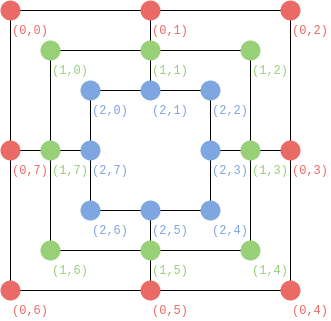
\includegraphics{../images/nmm-rings.png}

Die Spielpositionen (\texttt{cells}) \(c\) auf den Ringen sind beginnend
mit \(c=0\) ab der oberen linken Ecke im Uhrzeigersinn durch nummeriert.
Dadurch ergibt sich, dass \(c \in \{0...7\}\). In der Abbilung sind die
Koordinaten der Spielpositionen eingezeichnet, so liegt beispielsweise
\(\langle r,c \rangle = \langle 2,4 \rangle\) auf dem inneren Ring in
der unteren rechten Ecke. An diesen Spielpositionen wird der Spieler
\(p\) oder eine leere Spielposition gespeichert, für diese gilt
\(p \in Player \cup \{'\ '\}\).

So ist ein State eine Tupel \(\langle stash, board \rangle\) dessen
Parameter 

\begin{itemize}
    \item \texttt{stash} eine weitere Tupel, bestehend aus \(\langle w, b \rangle\) und
    \item \texttt{board} eine Tripel, welche die
    Ringe \(r_0\), \(r_1\) und \(r_2\) beinhaltet. Die Ringe selbst sind
    Neun-Tupel, dessen Elemente die einzelnen Spielpositionen
    \(c \in Player \cup \{'\ '\}\) darstellen.
\end{itemize}

Der Startzustand \(s_0\) wird in Python wie folgt geschrieben:

    \begin{tcolorbox}[breakable, size=fbox, boxrule=1pt, pad at break*=1mm,colback=cellbackground, colframe=cellborder]
\prompt{In}{incolor}{ }{\boxspacing}
\begin{Verbatim}[commandchars=\\\{\}]
\PY{n}{s0} \PY{o}{=} \PY{p}{(}\PY{p}{(}\PY{l+m+mi}{9}\PY{p}{,} \PY{l+m+mi}{9}\PY{p}{)}\PY{p}{,} \PY{p}{(}
    \PY{p}{(}\PY{l+s+s1}{\PYZsq{}}\PY{l+s+s1}{ }\PY{l+s+s1}{\PYZsq{}}\PY{p}{,} \PY{l+s+s1}{\PYZsq{}}\PY{l+s+s1}{ }\PY{l+s+s1}{\PYZsq{}}\PY{p}{,} \PY{l+s+s1}{\PYZsq{}}\PY{l+s+s1}{ }\PY{l+s+s1}{\PYZsq{}}\PY{p}{,} \PY{l+s+s1}{\PYZsq{}}\PY{l+s+s1}{ }\PY{l+s+s1}{\PYZsq{}}\PY{p}{,} \PY{l+s+s1}{\PYZsq{}}\PY{l+s+s1}{ }\PY{l+s+s1}{\PYZsq{}}\PY{p}{,} \PY{l+s+s1}{\PYZsq{}}\PY{l+s+s1}{ }\PY{l+s+s1}{\PYZsq{}}\PY{p}{,} \PY{l+s+s1}{\PYZsq{}}\PY{l+s+s1}{ }\PY{l+s+s1}{\PYZsq{}}\PY{p}{,} \PY{l+s+s1}{\PYZsq{}}\PY{l+s+s1}{ }\PY{l+s+s1}{\PYZsq{}}\PY{p}{)}\PY{p}{,}
    \PY{p}{(}\PY{l+s+s1}{\PYZsq{}}\PY{l+s+s1}{ }\PY{l+s+s1}{\PYZsq{}}\PY{p}{,} \PY{l+s+s1}{\PYZsq{}}\PY{l+s+s1}{ }\PY{l+s+s1}{\PYZsq{}}\PY{p}{,} \PY{l+s+s1}{\PYZsq{}}\PY{l+s+s1}{ }\PY{l+s+s1}{\PYZsq{}}\PY{p}{,} \PY{l+s+s1}{\PYZsq{}}\PY{l+s+s1}{ }\PY{l+s+s1}{\PYZsq{}}\PY{p}{,} \PY{l+s+s1}{\PYZsq{}}\PY{l+s+s1}{ }\PY{l+s+s1}{\PYZsq{}}\PY{p}{,} \PY{l+s+s1}{\PYZsq{}}\PY{l+s+s1}{ }\PY{l+s+s1}{\PYZsq{}}\PY{p}{,} \PY{l+s+s1}{\PYZsq{}}\PY{l+s+s1}{ }\PY{l+s+s1}{\PYZsq{}}\PY{p}{,} \PY{l+s+s1}{\PYZsq{}}\PY{l+s+s1}{ }\PY{l+s+s1}{\PYZsq{}}\PY{p}{)}\PY{p}{,}
    \PY{p}{(}\PY{l+s+s1}{\PYZsq{}}\PY{l+s+s1}{ }\PY{l+s+s1}{\PYZsq{}}\PY{p}{,} \PY{l+s+s1}{\PYZsq{}}\PY{l+s+s1}{ }\PY{l+s+s1}{\PYZsq{}}\PY{p}{,} \PY{l+s+s1}{\PYZsq{}}\PY{l+s+s1}{ }\PY{l+s+s1}{\PYZsq{}}\PY{p}{,} \PY{l+s+s1}{\PYZsq{}}\PY{l+s+s1}{ }\PY{l+s+s1}{\PYZsq{}}\PY{p}{,} \PY{l+s+s1}{\PYZsq{}}\PY{l+s+s1}{ }\PY{l+s+s1}{\PYZsq{}}\PY{p}{,} \PY{l+s+s1}{\PYZsq{}}\PY{l+s+s1}{ }\PY{l+s+s1}{\PYZsq{}}\PY{p}{,} \PY{l+s+s1}{\PYZsq{}}\PY{l+s+s1}{ }\PY{l+s+s1}{\PYZsq{}}\PY{p}{,} \PY{l+s+s1}{\PYZsq{}}\PY{l+s+s1}{ }\PY{l+s+s1}{\PYZsq{}}\PY{p}{)}
\PY{p}{)}\PY{p}{)}
\end{Verbatim}
\end{tcolorbox}

    \hypertarget{folgezustuxe4nde}{%
\subsection{Folgezustände}\label{folgezustuxe4nde}}

Für die Definition des Spieles Mühle \(G_{Nine Men's Morris}\) wird die
Funktion \texttt{nextStates} benötigt. Diese nimmt einen Zustand
\texttt{s} und einen Spieler \texttt{p} entgegen und errechnet mit
diesen alle Folgezustände, die entstehen, wenn der gegebene Spieler
einen legalen Zug spielt.

Da das Spiel in drei Phasen aufgeteilt ist, ist auch die Implementierung
aus Gründen der Übersicht in die folgenden Phasen unterteilt:

\begin{enumerate}
    \item Die
    erste Phase des Spiels heißt \emph{placing} Phase, in der die Spieler
    alle ihre Steine aus dem Stapel auf das Spielbrett legen müssen. Hierbei
    dürfen bereits Mühlen gelegt und geschlagen werden. Es muss ein Stein
    platziert werden.
    \item Die zweite Phase heißt \emph{moving} Phase und
    beginnt sobald der Stapel des Spielers leer ist. Beide Spieler kommen
    gleichzeitig in die zweite Phase, in der die eigenen Steine nur noch
    entlang der Linien auf die nächste Spielposition geschoben werden
    dürfen. Es muss ein Stein bewegt werden.
    \item Die letzte Phase heißt
    \emph{flying} Phase. Diese Phase beginnt für einen Spieler, sobald
    dieser nur noch \(3\) Steine auf dem Spielbrett liegen hat und sein
    Stapel leer ist. Der Eintritt in die dritte Phase ist nicht vom
    gegnerischen Spieler abhängig, somit können Spieler für mehrere Züge
    alleine in der dritten Phase sein. Hierbei können die verbleibenden
    Steine beliebig bewegt werden, ohne dass die Positionen direkt
    nebeneinander liegen müssen. Es muss ein Stein bewegt werden.
\end{enumerate}

In der ersten Phase, der \emph{placing} Phase, wird ein Stein vom Stapel
genommen und auf ein freies Feld gelegt. Diese Züge werden in der
Funktion \texttt{nextStatesPlace} implementiert, hierbei wird ein
Spieler \texttt{p} und ein Zustand \texttt{s} erwartet, für den
angenommen wird, dass sich der aktuelle Zustand in der ersten Phase
befindet. Die Rückgabe dieser Funktion ist die Menge aller Zustände, die
erreicht werden können, in denen der Spieler \texttt{p} einen legalen
Spielzug auf dem Zustand \texttt{s} ausführt.

\begin{enumerate}
\def\labelenumi{\arabic{enumi}.}
\tightlist
\item
  Zunächst werden die Mühlen aus dem aktuellen Zustand mit Hilfe der
  Funktion \texttt{findMills} gespeichert.
\item
  Daraufhin wird auf jede freie Spielposition ein neuer Stein des
  Spielers \texttt{p} gelegt.
\item
  Nun werden unter Verwendung von dem Ergebnis aus \emph{1.} und der
  Funktion \texttt{countNewMills} alle neu entstandenen Mühlen gezählt.
  Für diese Anzahl gilt \(a \in \{0,1,2\}\).
\item
  Um für die neu entstandenen Mühlen die entsprechende Anzahl an Steinen
  zu schlagen, wird die Hilfsfunktion \texttt{poundMills} verwendet.
\item
  Zum Schluss wird vom Stapel des Spielers \texttt{p} ein Stein weg
  genommen und der Stapel mit den Spielbrettern wieder zu Zuständen
  vereint.
\end{enumerate}

    \begin{tcolorbox}[breakable, size=fbox, boxrule=1pt, pad at break*=1mm,colback=cellbackground, colframe=cellborder]
\prompt{In}{incolor}{ }{\boxspacing}
\begin{Verbatim}[commandchars=\\\{\}]
\PY{k}{def} \PY{n+nf}{nextStatesPlace}\PY{p}{(}\PY{n}{s}\PY{p}{,} \PY{n}{p}\PY{p}{)}\PY{p}{:}
    \PY{c+c1}{\PYZsh{} Extract the count of the stones and the board}
    \PY{p}{(}\PY{p}{(}\PY{n}{cw}\PY{p}{,} \PY{n}{cb}\PY{p}{)}\PY{p}{,} \PY{n}{board}\PY{p}{)} \PY{o}{=} \PY{n}{s}
    \PY{c+c1}{\PYZsh{} Calculate all current mills the player has}
    \PY{n}{mills} \PY{o}{=} \PY{n}{findMills}\PY{p}{(}\PY{n}{board}\PY{p}{,} \PY{n}{p}\PY{p}{)}

    \PY{c+c1}{\PYZsh{} Place a stone in any empty cell}
    \PY{n}{placeBoards} \PY{o}{=} \PY{p}{\PYZob{}}
        \PY{n}{place}\PY{p}{(}\PY{n}{board}\PY{p}{,} \PY{p}{(}\PY{n}{r}\PY{p}{,} \PY{n}{c}\PY{p}{)}\PY{p}{,} \PY{n}{p}\PY{p}{)}
        \PY{k}{for} \PY{p}{(}\PY{n}{r}\PY{p}{,} \PY{n}{c}\PY{p}{)} \PY{o+ow}{in} \PY{n}{findEmptyCells}\PY{p}{(}\PY{n}{board}\PY{p}{)}
    \PY{p}{\PYZcb{}}
    \PY{c+c1}{\PYZsh{} Calculate how many new mills were created}
    \PY{n}{boardMills} \PY{o}{=} \PY{p}{\PYZob{}}
        \PY{n}{board}\PY{p}{:} \PY{n}{countNewMills}\PY{p}{(}\PY{n}{board}\PY{p}{,} \PY{n}{mills}\PY{p}{,} \PY{n}{p}\PY{p}{)}
        \PY{k}{for} \PY{n}{board} \PY{o+ow}{in} \PY{n}{placeBoards}
    \PY{p}{\PYZcb{}}

    \PY{c+c1}{\PYZsh{} Here all final boards will be collected}
    \PY{n}{boards} \PY{o}{=} \PY{p}{\PYZob{}}
        \PY{n}{result}
        \PY{k}{for} \PY{p}{(}\PY{n}{b}\PY{p}{,} \PY{n}{count}\PY{p}{)} \PY{o+ow}{in} \PY{n}{boardMills}\PY{o}{.}\PY{n}{items}\PY{p}{(}\PY{p}{)} 
        \PY{k}{for} \PY{n}{result} \PY{o+ow}{in} \PY{n}{poundMills}\PY{p}{(}\PY{n}{b}\PY{p}{,} \PY{n}{count}\PY{p}{,} \PY{n}{p}\PY{p}{)}
    \PY{p}{\PYZcb{}}

    \PY{c+c1}{\PYZsh{} Remove one stone from the players stache}
    \PY{p}{(}\PY{n}{cw}\PY{p}{,} \PY{n}{cb}\PY{p}{)} \PY{o}{=} \PY{p}{(}\PY{n}{cw}\PY{o}{\PYZhy{}}\PY{l+m+mi}{1}\PY{p}{,} \PY{n}{cb}\PY{p}{)} \PY{k}{if} \PY{n}{p} \PY{o}{==} \PY{l+s+s1}{\PYZsq{}}\PY{l+s+s1}{w}\PY{l+s+s1}{\PYZsq{}} \PY{k}{else} \PY{p}{(}\PY{n}{cw}\PY{p}{,} \PY{n}{cb}\PY{o}{\PYZhy{}}\PY{l+m+mi}{1}\PY{p}{)}

    \PY{c+c1}{\PYZsh{} Return all possible states}
    \PY{k}{return} \PY{p}{\PYZob{}} \PY{p}{(}\PY{p}{(}\PY{n}{cw}\PY{p}{,} \PY{n}{cb}\PY{p}{)}\PY{p}{,} \PY{n}{board}\PY{p}{)} \PY{k}{for} \PY{n}{board} \PY{o+ow}{in} \PY{n}{boards} \PY{p}{\PYZcb{}}
\end{Verbatim}
\end{tcolorbox}

    In der \emph{moving} Phase (2) wird ein Stein des aktuellen Spielers
entlang der Linien zu einer benachbarten, leeren Spielposition
geschoben. Die Definition der Funktion \texttt{nextStatesMove} wird
wieder eine Zustand \texttt{s} und ein Spieler \texttt{p} erwartet, die
sich in der zweiten Phase befinden. Die Rückgabe dieser Funktion ist die
Menge aller Zustände, die erreicht werden können, in denen der Spieler
\texttt{p} einen legalen Spielzug auf dem Zustand \texttt{s} ausführt.

\begin{enumerate}
\def\labelenumi{\arabic{enumi}.}
\tightlist
\item
  Zunächst werden die Mühlen aus dem aktuellen Zustand mit Hilfe der
  Funktion \texttt{findMills} gespeichert.
\item
  Danach werden die Positionen aller Steine des Spielers \texttt{p} und
  dessen leere Nachbarpositionen mit Hilfe der Funktionen
  \texttt{findCellsOf} und \texttt{findNeighboringEmptyCells} errechnet.
  Die Steine werden dort hin bewegt.
\item
  Nun werden unter Verwendung von dem Ergebnis aus \emph{1.} und der
  Funktion \texttt{countNewMills} alle neu entstandenen Mühlen gezählt.
  Für diese Anzahl gilt \(a \in \{0,1\}\).
\item
  Um für die neu entstandenen Mühlen die entsprechende Anzahl an Steinen
  zu schlagen, wird die Hilfsfunktion \texttt{poundMills} verwendet.
\item
  Zum Schluss wird der Stapel mit den Spielbrettern wieder zu Zuständen
  vereint.
\end{enumerate}

    \begin{tcolorbox}[breakable, size=fbox, boxrule=1pt, pad at break*=1mm,colback=cellbackground, colframe=cellborder]
\prompt{In}{incolor}{ }{\boxspacing}
\begin{Verbatim}[commandchars=\\\{\}]
\PY{k}{def} \PY{n+nf}{nextStatesMove}\PY{p}{(}\PY{n}{s}\PY{p}{,} \PY{n}{p}\PY{p}{)}\PY{p}{:}
    \PY{c+c1}{\PYZsh{} Extract the count of the stones and the board}
    \PY{p}{(}\PY{p}{(}\PY{n}{cw}\PY{p}{,} \PY{n}{cb}\PY{p}{)}\PY{p}{,} \PY{n}{board}\PY{p}{)} \PY{o}{=} \PY{n}{s}
    \PY{c+c1}{\PYZsh{} Calculate all current mills the player has}
    \PY{n}{mills} \PY{o}{=} \PY{n}{findMills}\PY{p}{(}\PY{n}{board}\PY{p}{,} \PY{n}{p}\PY{p}{)}

    \PY{c+c1}{\PYZsh{} Choose any stone of the player and move it to an empty neighbor}
    \PY{n}{moveBoards} \PY{o}{=} \PY{p}{\PYZob{}}
        \PY{n}{move}\PY{p}{(}\PY{n}{board}\PY{p}{,} \PY{n}{src}\PY{p}{,} \PY{n}{des}\PY{p}{)}
        \PY{k}{for} \PY{n}{src} \PY{o+ow}{in} \PY{n}{findCellsOf}\PY{p}{(}\PY{n}{board}\PY{p}{,} \PY{n}{p}\PY{p}{)}
        \PY{k}{for} \PY{n}{des} \PY{o+ow}{in} \PY{n}{findNeighboringEmptyCells}\PY{p}{(}\PY{n}{board}\PY{p}{,} \PY{n}{src}\PY{p}{)}
    \PY{p}{\PYZcb{}}

    \PY{c+c1}{\PYZsh{} Calculate how many new mills were created}
    \PY{n}{boardMills} \PY{o}{=} \PY{p}{\PYZob{}}
        \PY{n}{b}\PY{p}{:} \PY{n}{countNewMills}\PY{p}{(}\PY{n}{b}\PY{p}{,} \PY{n}{mills}\PY{p}{,} \PY{n}{p}\PY{p}{)}
        \PY{k}{for} \PY{n}{b} \PY{o+ow}{in} \PY{n}{moveBoards}
    \PY{p}{\PYZcb{}}

    \PY{c+c1}{\PYZsh{} Here all final boards will be collected}
    \PY{n}{boards} \PY{o}{=} \PY{p}{\PYZob{}}
        \PY{n}{result}
        \PY{k}{for} \PY{p}{(}\PY{n}{b}\PY{p}{,} \PY{n}{count}\PY{p}{)} \PY{o+ow}{in} \PY{n}{boardMills}\PY{o}{.}\PY{n}{items}\PY{p}{(}\PY{p}{)} 
        \PY{k}{for} \PY{n}{result} \PY{o+ow}{in} \PY{n}{poundMills}\PY{p}{(}\PY{n}{b}\PY{p}{,} \PY{n}{count}\PY{p}{,} \PY{n}{p}\PY{p}{)}
    \PY{p}{\PYZcb{}}

    \PY{k}{return} \PY{p}{\PYZob{}} \PY{p}{(}\PY{p}{(}\PY{n}{cw}\PY{p}{,} \PY{n}{cb}\PY{p}{)}\PY{p}{,} \PY{n}{board}\PY{p}{)} \PY{k}{for} \PY{n}{board} \PY{o+ow}{in} \PY{n}{boards} \PY{p}{\PYZcb{}}
\end{Verbatim}
\end{tcolorbox}

    Die letzte Hilfsfunktion \texttt{nextStatesFly} wird in der Phase 3
verwendet und erwartet äquivalent zu den anderen Hilfsmethoden einen
Zustand \texttt{s} und Spieler \texttt{p} in der Phase 3. Hier wird ein
Stein des Spieler \texttt{p} an eine andere Position auf dem Spielbrett
bewegt. Diese Position muss keine Nachbarposition sein und Steine können
übersprungen werden. Die Rückgabe dieser Funktion ist die Menge aller
Zustände, die erreicht werden können, in denen der Spieler \texttt{p}
einen legalen Spielzug auf dem Zustand \texttt{s} ausführt.

\begin{enumerate}
\def\labelenumi{\arabic{enumi}.}
\tightlist
\item
  Zunächst werden die Mühlen aus dem aktuellen Zustand mit Hilfe der
  Funktion \texttt{findMills} gespeichert.
\item
  Danach werden die Positionen aller Steine des Spielers \texttt{p} und
  dessen leere Nachbarpositionen mit Hilfe der Funktionen
  \texttt{findCellsOf} und \texttt{findNeighboringEmptyCells} errechnet.
  Die Steine werden dort hin bewegt.
\item
  Nun werden unter Verwendung von dem Ergebnis aus \emph{1.} und der
  Funktion \texttt{countNewMills} alle neu entstandenen Mühlen gezählt.
  Für diese Anzahl gilt \(a \in \{0,1\}\).
\item
  Um für die neu entstandenen Mühlen die entsprechende Anzahl an Steinen
  zu schlagen, wird die Hilfsfunktion \texttt{poundMills} verwendet.
\item
  Zum Schluss wird der Stapel mit den Spielbrettern wieder zu Zuständen
  vereint.
\end{enumerate}

    \begin{tcolorbox}[breakable, size=fbox, boxrule=1pt, pad at break*=1mm,colback=cellbackground, colframe=cellborder]
\prompt{In}{incolor}{ }{\boxspacing}
\begin{Verbatim}[commandchars=\\\{\}]
\PY{k}{def} \PY{n+nf}{nextStatesFly}\PY{p}{(}\PY{n}{s}\PY{p}{,} \PY{n}{p}\PY{p}{)}\PY{p}{:}
    \PY{c+c1}{\PYZsh{} Extract the count of the stones and the board}
    \PY{p}{(}\PY{p}{(}\PY{n}{cw}\PY{p}{,} \PY{n}{cb}\PY{p}{)}\PY{p}{,} \PY{n}{board}\PY{p}{)} \PY{o}{=} \PY{n}{s}
    \PY{c+c1}{\PYZsh{} Calculate all current mills the player has}
    \PY{n}{mills} \PY{o}{=} \PY{n}{findMills}\PY{p}{(}\PY{n}{board}\PY{p}{,} \PY{n}{p}\PY{p}{)}

    \PY{c+c1}{\PYZsh{} Choose any stone of the player and move it to an empty neighbor}
    \PY{n}{moveBoards} \PY{o}{=} \PY{p}{\PYZob{}}
        \PY{n}{move}\PY{p}{(}\PY{n}{board}\PY{p}{,} \PY{n}{src}\PY{p}{,} \PY{n}{des}\PY{p}{)}
        \PY{k}{for} \PY{n}{src} \PY{o+ow}{in} \PY{n}{findCellsOf}\PY{p}{(}\PY{n}{board}\PY{p}{,} \PY{n}{p}\PY{p}{)}
        \PY{k}{for} \PY{n}{des} \PY{o+ow}{in} \PY{n}{findEmptyCells}\PY{p}{(}\PY{n}{board}\PY{p}{)}
    \PY{p}{\PYZcb{}}

    \PY{c+c1}{\PYZsh{} Calculate how many new mills were created}
    \PY{n}{boardMills} \PY{o}{=} \PY{p}{\PYZob{}}
        \PY{n}{b}\PY{p}{:} \PY{n}{countNewMills}\PY{p}{(}\PY{n}{b}\PY{p}{,} \PY{n}{mills}\PY{p}{,} \PY{n}{p}\PY{p}{)}
        \PY{k}{for} \PY{n}{b} \PY{o+ow}{in} \PY{n}{moveBoards}
    \PY{p}{\PYZcb{}}

    \PY{c+c1}{\PYZsh{} Here all final boards will be collected}
    \PY{n}{boards} \PY{o}{=} \PY{p}{\PYZob{}}
        \PY{n}{result}
        \PY{k}{for} \PY{p}{(}\PY{n}{b}\PY{p}{,} \PY{n}{count}\PY{p}{)} \PY{o+ow}{in} \PY{n}{boardMills}\PY{o}{.}\PY{n}{items}\PY{p}{(}\PY{p}{)} 
        \PY{k}{for} \PY{n}{result} \PY{o+ow}{in} \PY{n}{poundMills}\PY{p}{(}\PY{n}{b}\PY{p}{,} \PY{n}{count}\PY{p}{,} \PY{n}{p}\PY{p}{)}
    \PY{p}{\PYZcb{}}

    \PY{k}{return} \PY{p}{\PYZob{}} \PY{p}{(}\PY{p}{(}\PY{n}{cw}\PY{p}{,} \PY{n}{cb}\PY{p}{)}\PY{p}{,} \PY{n}{board}\PY{p}{)} \PY{k}{for} \PY{n}{board} \PY{o+ow}{in} \PY{n}{boards} \PY{p}{\PYZcb{}}
\end{Verbatim}
\end{tcolorbox}

    Die Implementierung der \texttt{nextStates} Funktion führt nun die
vorher definierten Funktionen zusammen. Die aktuelle Phase für den
gegebenen Zustand \texttt{s} und Spieler \texttt{p} wird mit der
Hilfsfunktion \texttt{playerPhase} errechnet und auf Grund dessen eine
Fallunterscheidung ausgeführt, sodass gilt

\[
nextStates(s, p) = \begin{cases}
nextStatesPlace(s, p) & falls\ \  playerPhase(s, p) = 1 \\
nextStatesMove(s, p) & falls\ \  playerPhase(s, p) = 2 \\
nextStatesFly(s, p) & falls\ \  playerPhase(s, p) = 3
\end{cases}
\]

    \begin{tcolorbox}[breakable, size=fbox, boxrule=1pt, pad at break*=1mm,colback=cellbackground, colframe=cellborder]
\prompt{In}{incolor}{ }{\boxspacing}
\begin{Verbatim}[commandchars=\\\{\}]
\PY{k}{def} \PY{n+nf}{nextStates}\PY{p}{(}\PY{n}{s}\PY{p}{,} \PY{n}{p}\PY{p}{)}\PY{p}{:}
    \PY{n}{phase} \PY{o}{=} \PY{n}{playerPhase}\PY{p}{(}\PY{n}{s}\PY{p}{,} \PY{n}{p}\PY{p}{)}
    \PY{k}{if} \PY{n}{phase} \PY{o}{==} \PY{l+m+mi}{1}\PY{p}{:}
        \PY{k}{return} \PY{n}{nextStatesPlace}\PY{p}{(}\PY{n}{s}\PY{p}{,} \PY{n}{p}\PY{p}{)}
    \PY{k}{elif} \PY{n}{phase} \PY{o}{==} \PY{l+m+mi}{2}\PY{p}{:}
        \PY{k}{return} \PY{n}{nextStatesMove}\PY{p}{(}\PY{n}{s}\PY{p}{,} \PY{n}{p}\PY{p}{)}
    \PY{k}{else}\PY{p}{:}
        \PY{k}{return} \PY{n}{nextStatesFly}\PY{p}{(}\PY{n}{s}\PY{p}{,} \PY{n}{p}\PY{p}{)}
\end{Verbatim}
\end{tcolorbox}

    \hypertarget{spielende}{%
\subsection{Spielende}\label{spielende}}

    Für die Definition des Spieles Mühle \(G_{Nine Men's Morris}\) werden
zwei weitere Funktionen benötigt, die das Ende des Spiels behandeln:
\texttt{finished} und \texttt{utility}.

Die Funktion \texttt{finished} errechnet für einen gegebenen Zustand
\texttt{s}, ob das Spiel beendet ist, wenn Spieler \texttt{p} an der
Reihe ist. Dies ist der Fall, g.d.w.

\begin{itemize}
    \item einer der Spieler
    \(p \in Players\) weniger als 3 Steine hat (\texttt{hasEnoughStones})
    oder
    \item der Spieler \texttt{p} keinen legalen Zug mehr tätigen kann.
\end{itemize}

Der optionale Parameter \texttt{ns} ist lediglich eine Optimierung, die
es ermöglicht, bereits berechnete Folgezustände zu verwenden, anstatt
diese noch einmal errechnen lassen zu müssen.

    \begin{tcolorbox}[breakable, size=fbox, boxrule=1pt, pad at break*=1mm,colback=cellbackground, colframe=cellborder]
\prompt{In}{incolor}{ }{\boxspacing}
\begin{Verbatim}[commandchars=\\\{\}]
\PY{k}{def} \PY{n+nf}{finished}\PY{p}{(}\PY{n}{s}\PY{p}{,} \PY{n}{p}\PY{p}{,} \PY{n}{ns}\PY{o}{=}\PY{k+kc}{None}\PY{p}{)}\PY{p}{:}
    \PY{k}{if} \PY{o+ow}{not} \PY{n}{ns}\PY{p}{:}
        \PY{n}{ns} \PY{o}{=} \PY{n}{nextStates}\PY{p}{(}\PY{n}{s}\PY{p}{,} \PY{n}{p}\PY{p}{)}\PY{p}{;}
    \PY{k}{return} \PY{o+ow}{not} \PY{n}{hasEnoughStones}\PY{p}{(}\PY{n}{s}\PY{p}{,} \PY{l+s+s1}{\PYZsq{}}\PY{l+s+s1}{w}\PY{l+s+s1}{\PYZsq{}}\PY{p}{)} \PY{o+ow}{or} \PYZbs{}
           \PY{o+ow}{not} \PY{n}{hasEnoughStones}\PY{p}{(}\PY{n}{s}\PY{p}{,} \PY{l+s+s1}{\PYZsq{}}\PY{l+s+s1}{b}\PY{l+s+s1}{\PYZsq{}}\PY{p}{)} \PY{o+ow}{or} \PYZbs{}
           \PY{n+nb}{len}\PY{p}{(}\PY{n}{ns}\PY{p}{)} \PY{o}{==} \PY{l+m+mi}{0}
\end{Verbatim}
\end{tcolorbox}

    Die Funktion \texttt{utility} errechnet für den gegebenen Zustand
\texttt{s} und Spieler \texttt{p}, falls \(finished(s, p) = true\) gilt,
wer gewonnen hat.

\[
utility(s, p) = \begin{cases}
-1 & falls\ \  p \ verliert \ in \ s \\
 0 & falls\ \  Unentschieden         \\
 1 & falls\ \  p \ gewinnt  \ in \ s
\end{cases}
\]

Sobald ein Spieler zu wenig Steine hat (\texttt{hasEnoughStones}) oder
keinen legalen Zug mehr tätigen kann, hat dieser verloren. Dadurch
gewinnt automatisch der gegnerische Spieler. Zwar gibt es im Spiel Mühle
ein Unentschieden, dies kann aber nicht anhand der Zustände erkannt
werden, da hierbei die vorher gespielten Spielzüge betrachtet werden
müssen.

Äquivalent zu der Funktion \texttt{finished} ist Parameter \texttt{ns}
optional und stellt lediglich eine Optimierung dar, die es ermöglicht,
bereits berechnete Folgezustände zu verwenden, anstatt diese noch einmal
errechnen lassen zu müssen.

    \begin{tcolorbox}[breakable, size=fbox, boxrule=1pt, pad at break*=1mm,colback=cellbackground, colframe=cellborder]
\prompt{In}{incolor}{ }{\boxspacing}
\begin{Verbatim}[commandchars=\\\{\}]
\PY{k}{def} \PY{n+nf}{utility}\PY{p}{(}\PY{n}{s}\PY{p}{,} \PY{n}{p}\PY{p}{,} \PY{n}{ns}\PY{o}{=}\PY{k+kc}{None}\PY{p}{)}\PY{p}{:}
    \PY{k}{if} \PY{o+ow}{not} \PY{n}{ns}\PY{p}{:}
        \PY{n}{ns} \PY{o}{=} \PY{n}{nextStates}\PY{p}{(}\PY{n}{s}\PY{p}{,} \PY{n}{p}\PY{p}{)}\PY{p}{;}
     
    \PY{k}{if} \PY{o+ow}{not} \PY{n}{hasEnoughStones}\PY{p}{(}\PY{n}{s}\PY{p}{,} \PY{n}{p}\PY{p}{)}\PY{p}{:}
        \PY{k}{return} \PY{o}{\PYZhy{}}\PY{l+m+mi}{1}
    \PY{k}{if} \PY{o+ow}{not} \PY{n}{hasEnoughStones}\PY{p}{(}\PY{n}{s}\PY{p}{,} \PY{n}{opponent}\PY{p}{(}\PY{n}{p}\PY{p}{)}\PY{p}{)}\PY{p}{:}
        \PY{k}{return} \PY{l+m+mi}{1}
    \PY{k}{if} \PY{n+nb}{len}\PY{p}{(}\PY{n}{nextStates}\PY{p}{(}\PY{n}{s}\PY{p}{,} \PY{n}{p}\PY{p}{)}\PY{p}{)} \PY{o}{==} \PY{l+m+mi}{0}\PY{p}{:}
        \PY{k}{return} \PY{o}{\PYZhy{}}\PY{l+m+mi}{1}

    \PY{c+c1}{\PYZsh{} Should be impossible, as utility() will only be called if finished() returns True}
    \PY{k}{return} \PY{l+m+mi}{0}
\end{Verbatim}
\end{tcolorbox}


    % Add a bibliography block to the postdoc
    
    
    
    
    
    

    
    \hypertarget{kuxfcnstliche-intelligenz}{%
\section{Künstliche Intelligenz}\label{kuxfcnstliche-intelligenz}}

Diese Studienarbeit implementiert zwei verschiedene Algorithmen als
künstliche Intelligenz: Minimax und $\alpha$-$\beta$-Pruning. Damit diese Algorithmen
leichter wiederverwendet und mit verschiedenen Einstellungen ausgeführt
werden können, wird eine abstrakte Superklasse angelegt. Diese bescheibt
welche Funktionen nötig sind, damit eine Implementierung den Ansprüchen
einer künstlichen Intelligenz für Mühle entspricht.


    \hypertarget{bestmoves}{%
\subsection{BestMoves}\label{bestmoves}}

    Die Klasse \texttt{BestMoves} beschreibt das Ergebnis, welches eine
künstliche Intelligenz für Mühle erzeugen soll. Diese Klasse beschreibt
den Rückgabewert der später definierten Funktion \texttt{bestMoves}. Sie
hat drei Attribute:

\begin{itemize}
\tightlist
\item
  \texttt{states} \(\subset States\);
\item
  \texttt{value} \(\in \mathopen[-1.0,1.0\mathclose]\);
\item
  \texttt{debugInformation} ist ein \texttt{dict}, welches weitere
  Informationen, wie beispielsweise die erreichte Rekursionstiefe oder
  die besuchten Zustände, beinhalten kann.
\end{itemize}

    \begin{tcolorbox}[breakable, size=fbox, boxrule=1pt, pad at break*=1mm,colback=cellbackground, colframe=cellborder]
\prompt{In}{incolor}{ }{\boxspacing}
\begin{Verbatim}[commandchars=\\\{\}]
\PY{k}{class} \PY{n+nc}{BestMoves}\PY{p}{(}\PY{p}{)}\PY{p}{:}
    \PY{k}{def} \PY{n+nf+fm}{\PYZus{}\PYZus{}init\PYZus{}\PYZus{}}\PY{p}{(}\PY{n+nb+bp}{self}\PY{p}{,} \PY{n}{states}\PY{p}{,} \PY{n}{value}\PY{p}{,} \PY{n}{debugInformation}\PY{p}{)}\PY{p}{:}
        \PY{n+nb+bp}{self}\PY{o}{.}\PY{n}{states} \PY{o}{=} \PY{n}{states}
        \PY{n+nb+bp}{self}\PY{o}{.}\PY{n}{value} \PY{o}{=} \PY{n}{value}
        \PY{n+nb+bp}{self}\PY{o}{.}\PY{n}{debugInformation} \PY{o}{=} \PY{n}{debugInformation}
\end{Verbatim}
\end{tcolorbox}

    Für Entwicklungszwecke wird eine Stringdarstellung für die Klasse
\texttt{BestMoves} implementiert. Hierzu wird durch die Funktion
\texttt{\_\_repr\_\_} ein String zurückgegeben, der alle Parameter der
Klasse beinhaltet.

    \begin{tcolorbox}[breakable, size=fbox, boxrule=1pt, pad at break*=1mm,colback=cellbackground, colframe=cellborder]
\prompt{In}{incolor}{ }{\boxspacing}
\begin{Verbatim}[commandchars=\\\{\}]
\PY{k}{def} \PY{n+nf+fm}{\PYZus{}\PYZus{}repr\PYZus{}\PYZus{}}\PY{p}{(}\PY{n+nb+bp}{self}\PY{p}{)}\PY{p}{:}
    \PY{k}{return} \PY{l+s+sa}{f}\PY{l+s+s2}{\PYZdq{}}\PY{l+s+s2}{BestMoves(states=}\PY{l+s+si}{\PYZob{}}\PY{n+nb+bp}{self}\PY{o}{.}\PY{n}{states}\PY{l+s+si}{\PYZcb{}}\PY{l+s+s2}{, value=}\PY{l+s+si}{\PYZob{}}\PY{n+nb+bp}{self}\PY{o}{.}\PY{n}{value}\PY{l+s+si}{\PYZcb{}}\PY{l+s+s2}{, debugInformation=}\PY{l+s+si}{\PYZob{}}\PY{n+nb+bp}{self}\PY{o}{.}\PY{n}{debugInformation}\PY{l+s+si}{\PYZcb{}}\PY{l+s+s2}{)}\PY{l+s+s2}{\PYZdq{}}

\PY{n}{BestMoves}\PY{o}{.}\PY{n+nf+fm}{\PYZus{}\PYZus{}repr\PYZus{}\PYZus{}} \PY{o}{=} \PY{n+nf+fm}{\PYZus{}\PYZus{}repr\PYZus{}\PYZus{}}
\PY{k}{del} \PY{n+nf+fm}{\PYZus{}\PYZus{}repr\PYZus{}\PYZus{}}
\end{Verbatim}
\end{tcolorbox}

    Die Funktion \texttt{choice} wählt zufällig einen der möglichen besten
Züge aus einer \texttt{BestMoves} Instanz aus. Dadurch wird
sichergestellt, dass nicht immer der gleiche Zug durch die künstliche
Intelligenz gespielt wird.

    \begin{tcolorbox}[breakable, size=fbox, boxrule=1pt, pad at break*=1mm,colback=cellbackground, colframe=cellborder]
\prompt{In}{incolor}{ }{\boxspacing}
\begin{Verbatim}[commandchars=\\\{\}]
\PY{k+kn}{import} \PY{n+nn}{random}
\PY{k}{def} \PY{n+nf}{choice}\PY{p}{(}\PY{n+nb+bp}{self}\PY{p}{)}\PY{p}{:}
    \PY{k}{return} \PY{n}{random}\PY{o}{.}\PY{n}{choice}\PY{p}{(}\PY{n+nb+bp}{self}\PY{o}{.}\PY{n}{states}\PY{p}{)}

\PY{n}{BestMoves}\PY{o}{.}\PY{n}{choice} \PY{o}{=} \PY{n}{choice}
\PY{k}{del} \PY{n}{choice}
\end{Verbatim}
\end{tcolorbox}

    \hypertarget{artificialintelligence}{%
\subsection{ArtificialIntelligence}\label{artificialintelligence}}

    Für die Definition der abstrakten Superklasse müssen zunächst aus dem
Paket \texttt{abc} \emph{Abstract Base Classes} Hilfsklassen und
-funktionen importiert werden. Diese werden benötigt um eine abstrakte
Klassen in Python darstellen zu können.

    \begin{tcolorbox}[breakable, size=fbox, boxrule=1pt, pad at break*=1mm,colback=cellbackground, colframe=cellborder]
\prompt{In}{incolor}{ }{\boxspacing}
\begin{Verbatim}[commandchars=\\\{\}]
\PY{k+kn}{from} \PY{n+nn}{abc} \PY{k+kn}{import} \PY{n}{ABC}\PY{p}{,} \PY{n}{abstractmethod}
\end{Verbatim}
\end{tcolorbox}

    Die abstrakte Superklasse \texttt{ArtificialIntelligence} ist selbst
eine Unterklasse von \texttt{ABC}, dadurch wird die Klasse als abstrakt
markiert. \texttt{ArtificialIntelligence} hat eine abstrakte Funktion
\texttt{bestMoves}, die für einen Zustand und einen Spieler alle besten
Züge errechnen soll und diese in Form einer \texttt{BestMoves} Instanz
zurückgeben soll. Sie hat zwei Argumente:

\begin{itemize}
\tightlist
\item
  \texttt{states} \(\in States\);
\item
  \texttt{player} \(\in Players\).
\end{itemize}

    \begin{tcolorbox}[breakable, size=fbox, boxrule=1pt, pad at break*=1mm,colback=cellbackground, colframe=cellborder]
\prompt{In}{incolor}{ }{\boxspacing}
\begin{Verbatim}[commandchars=\\\{\}]
\PY{k}{class} \PY{n+nc}{ArtificialIntelligence}\PY{p}{(}\PY{n}{ABC}\PY{p}{)}\PY{p}{:}
    \PY{n+nd}{@abstractmethod}
    \PY{k}{def} \PY{n+nf}{bestMoves}\PY{p}{(}\PY{n+nb+bp}{self}\PY{p}{,} \PY{n}{state}\PY{p}{,} \PY{n}{player}\PY{p}{)} \PY{o}{\PYZhy{}}\PY{o}{\PYZgt{}} \PY{n}{BestMoves}\PY{p}{:}
        \PY{k}{pass}
\end{Verbatim}
\end{tcolorbox}


    % Add a bibliography block to the postdoc
    
    
    
    
    
    

    
    \hypertarget{heuristik}{%
\subsection{Heuristik}\label{heuristik}}

Da die Rechenleistung nicht ausreicht um vor jedem Zug den gesamten
Spielbaum abzusuchen, gibt es eine maximale Rekursionstiefe, bei der die
Suche abgebrochen wird. Wenn diese Rekusionstiefe erreicht wird, muss
der Wert des aktuellen Zustands geschätzt werden. Hierfür wird die in
diesem Kapitel beschriebene Heuristik verwendet.


    \begin{tcolorbox}[breakable, size=fbox, boxrule=1pt, pad at break*=1mm,colback=cellbackground, colframe=cellborder]
\prompt{In}{incolor}{ }{\boxspacing}
\begin{Verbatim}[commandchars=\\\{\}]
\PY{o}{\PYZpc{}}\PY{k}{run} ./nmm\PYZhy{}game.ipynb
\end{Verbatim}
\end{tcolorbox}

    Die Klasse \texttt{HeuristicWeights} ist eine Hilfsklasse, dessen
Instanzen beim Aufruf von der später definierten Funktion
\texttt{heuristic} übergeben werden können. In dieser Klasse werden alle
Gewichtungen für die einzelnen Eigenschaften eines Zustandes
gespeichert. Dadurch wird es ermöglicht künstliche Intelligenzen mit
verschiedenen Heuristiken gegeneinander antreten zu lassen, um
herauszufinden welche Heuristik den Wert eines Zustandes am genausten
abbildet.

Eine Instanz der Klasse \texttt{HeuristicWeights} besteht aus vier
Gewichtungen, eine für jede Eigenschaft:

\begin{itemize}
    \item \texttt{stones}: Diese Eigenschaft zählt, wie viele Steine der Spieler auf dem Spielbrett hat.
    \item \texttt{stash}: Die Steine auf dem Stapel werden ebenfalls gezählt.
    \item \texttt{mills}: Die Anzahl der Mühlen, die ein Spieler auf dem Spielbrett hat, wird durch diese Eigenschaft gezählt.
    \item \texttt{possible\_mills}: Die Anzahl der möglichen Mühlen, dh. Mühlen
    bei denen eine Zelle noch frei ist, werden ebenfalls gezählt. (Siehe
    \texttt{findPossibleMills} im Kapitel \emph{Hilfsfunktionen für die
    Spielimplementierung} für eine genauere Beschreibung einer möglichen
    Mühle.)
\end{itemize}

    \begin{tcolorbox}[breakable, size=fbox, boxrule=1pt, pad at break*=1mm,colback=cellbackground, colframe=cellborder]
\prompt{In}{incolor}{ }{\boxspacing}
\begin{Verbatim}[commandchars=\\\{\}]
\PY{k}{class} \PY{n+nc}{HeuristicWeights}\PY{p}{(}\PY{p}{)}\PY{p}{:}
    \PY{k}{def} \PY{n+nf+fm}{\PYZus{}\PYZus{}init\PYZus{}\PYZus{}}\PY{p}{(}\PY{n+nb+bp}{self}\PY{p}{,} \PY{n}{stones}\PY{o}{=}\PY{l+m+mi}{1}\PY{p}{,} \PY{n}{stash}\PY{o}{=}\PY{l+m+mi}{1}\PY{p}{,} \PY{n}{mills}\PY{o}{=}\PY{l+m+mi}{4}\PY{p}{,} \PY{n}{possible\PYZus{}mills}\PY{o}{=}\PY{l+m+mi}{2}\PY{p}{)}\PY{p}{:}
        \PY{n+nb+bp}{self}\PY{o}{.}\PY{n}{stones} \PY{o}{=} \PY{n}{stones}
        \PY{n+nb+bp}{self}\PY{o}{.}\PY{n}{stash} \PY{o}{=} \PY{n}{stash}
        \PY{n+nb+bp}{self}\PY{o}{.}\PY{n}{mills} \PY{o}{=} \PY{n}{mills}
        \PY{n+nb+bp}{self}\PY{o}{.}\PY{n}{possible\PYZus{}mills} \PY{o}{=} \PY{n}{possible\PYZus{}mills}
\end{Verbatim}
\end{tcolorbox}

    Für Debuggingzwecke wird eine \texttt{\_\_repr\_\_} Funktion
implementiert, die eine String-Repräsentation aus einer
\texttt{HeuristicWeights} Instanz mit allen Einstelungen erstellt.

    \begin{tcolorbox}[breakable, size=fbox, boxrule=1pt, pad at break*=1mm,colback=cellbackground, colframe=cellborder]
\prompt{In}{incolor}{ }{\boxspacing}
\begin{Verbatim}[commandchars=\\\{\}]
\PY{k}{def} \PY{n+nf+fm}{\PYZus{}\PYZus{}repr\PYZus{}\PYZus{}}\PY{p}{(}\PY{n+nb+bp}{self}\PY{p}{:} \PY{n}{HeuristicWeights}\PY{p}{)}\PY{p}{:}
    \PY{k}{return} \PY{l+s+sa}{f}\PY{l+s+s2}{\PYZdq{}}\PY{l+s+s2}{HeuristicWeights(stones=}\PY{l+s+si}{\PYZob{}}\PY{n+nb+bp}{self}\PY{o}{.}\PY{n}{stones}\PY{l+s+si}{\PYZcb{}}\PY{l+s+s2}{, stash=}\PY{l+s+si}{\PYZob{}}\PY{n+nb+bp}{self}\PY{o}{.}\PY{n}{stash}\PY{l+s+si}{\PYZcb{}}\PY{l+s+s2}{, }\PY{l+s+s2}{\PYZdq{}} \PY{o}{+} \PYZbs{}
           \PY{l+s+sa}{f}\PY{l+s+s2}{\PYZdq{}}\PY{l+s+s2}{mills=}\PY{l+s+si}{\PYZob{}}\PY{n+nb+bp}{self}\PY{o}{.}\PY{n}{mills}\PY{l+s+si}{\PYZcb{}}\PY{l+s+s2}{, possible\PYZus{}mills=}\PY{l+s+si}{\PYZob{}}\PY{n+nb+bp}{self}\PY{o}{.}\PY{n}{possible\PYZus{}mills}\PY{l+s+si}{\PYZcb{}}\PY{l+s+s2}{)}\PY{l+s+s2}{\PYZdq{}}

\PY{n}{HeuristicWeights}\PY{o}{.}\PY{n+nf+fm}{\PYZus{}\PYZus{}repr\PYZus{}\PYZus{}} \PY{o}{=} \PY{n+nf+fm}{\PYZus{}\PYZus{}repr\PYZus{}\PYZus{}}
\PY{k}{del} \PY{n+nf+fm}{\PYZus{}\PYZus{}repr\PYZus{}\PYZus{}}
\end{Verbatim}
\end{tcolorbox}

    Die Funktion \texttt{heuristic} berechnet für einen Spieler den
geschätzten Wert eines Zuststandes anhand der oben aufgeführten
Eigenschaften. Die Funktion hat drei Argumente:

\begin{itemize}
\tightlist
\item
  \texttt{state} \(\in States\);
\item
  \texttt{player} \(\in Players\);
\item
  optional: \texttt{weights} ist eine Instanz der Klasse
  \texttt{HeuristicWeights}.
\end{itemize}

Für die Implementierung werden alle gewichteten Werte der Eigenschaften
für die Spieler weiß \texttt{w} und schwarz \texttt{b}, sowie der
maximale Wert für die Eigenschaft errechnet. Damit die Schätzung des
Wertes nicht außerhalb des Wertebereiches, gegeben durch die
tatsächlichen Werte für gewinnende (\texttt{1.0}) und verlierende
(\texttt{-1.0}) Zustände, liegt, wird das Maximum um eins erhöht und der
errechnete Wert durch das Maximum skaliert. Zum Schluss wird das
Vorzeichen angepasst, damit der gegebene Spieler berücksichtigt wird.

    \begin{tcolorbox}[breakable, size=fbox, boxrule=1pt, pad at break*=1mm,colback=cellbackground, colframe=cellborder]
\prompt{In}{incolor}{ }{\boxspacing}
\begin{Verbatim}[commandchars=\\\{\}]
\PY{k}{def} \PY{n+nf}{heuristic}\PY{p}{(}\PY{n}{state}\PY{p}{,} \PY{n}{player}\PY{p}{,} \PY{n}{weights}\PY{o}{=}\PY{n}{HeuristicWeights}\PY{p}{(}\PY{p}{)}\PY{p}{)}\PY{p}{:}
    \PY{p}{(}\PY{p}{(}\PY{n}{stash\PYZus{}white}\PY{p}{,} \PY{n}{stash\PYZus{}black}\PY{p}{)}\PY{p}{,} \PY{n}{board}\PY{p}{)} \PY{o}{=} \PY{n}{state}
    
    \PY{c+c1}{\PYZsh{} Count the stones on the board}
    \PY{n}{white} \PY{o}{=} \PY{n}{weights}\PY{o}{.}\PY{n}{stones} \PY{o}{*} \PY{n}{countStones}\PY{p}{(}\PY{n}{state}\PY{p}{,} \PY{l+s+s1}{\PYZsq{}}\PY{l+s+s1}{w}\PY{l+s+s1}{\PYZsq{}}\PY{p}{)}
    \PY{n}{black} \PY{o}{=} \PY{n}{weights}\PY{o}{.}\PY{n}{stones} \PY{o}{*} \PY{n}{countStones}\PY{p}{(}\PY{n}{state}\PY{p}{,} \PY{l+s+s1}{\PYZsq{}}\PY{l+s+s1}{b}\PY{l+s+s1}{\PYZsq{}}\PY{p}{)}
    \PY{c+c1}{\PYZsh{} Count the stones in the stash}
    \PY{n}{white} \PY{o}{+}\PY{o}{=} \PY{n}{weights}\PY{o}{.}\PY{n}{stash} \PY{o}{*} \PY{n}{stash\PYZus{}white}
    \PY{n}{black} \PY{o}{+}\PY{o}{=} \PY{n}{weights}\PY{o}{.}\PY{n}{stash} \PY{o}{*} \PY{n}{stash\PYZus{}black}
    \PY{c+c1}{\PYZsh{} There can be at maximum 9 stones per player, so the maximum is the maximum of the weights times the stones}
    \PY{n}{maximum} \PY{o}{=} \PY{l+m+mi}{9} \PY{o}{*} \PY{n+nb}{max}\PY{p}{(}\PY{n}{weights}\PY{o}{.}\PY{n}{stones}\PY{p}{,} \PY{n}{weights}\PY{o}{.}\PY{n}{stash}\PY{p}{)}
    
    \PY{c+c1}{\PYZsh{} Count the mills the player currently has}
    \PY{n}{white} \PY{o}{+}\PY{o}{=} \PY{n}{weights}\PY{o}{.}\PY{n}{mills} \PY{o}{*} \PY{n+nb}{len}\PY{p}{(}\PY{n}{findMills}\PY{p}{(}\PY{n}{board}\PY{p}{,} \PY{l+s+s1}{\PYZsq{}}\PY{l+s+s1}{w}\PY{l+s+s1}{\PYZsq{}}\PY{p}{)}\PY{p}{)}
    \PY{n}{black} \PY{o}{+}\PY{o}{=} \PY{n}{weights}\PY{o}{.}\PY{n}{mills} \PY{o}{*} \PY{n+nb}{len}\PY{p}{(}\PY{n}{findMills}\PY{p}{(}\PY{n}{board}\PY{p}{,} \PY{l+s+s1}{\PYZsq{}}\PY{l+s+s1}{b}\PY{l+s+s1}{\PYZsq{}}\PY{p}{)}\PY{p}{)}
    \PY{c+c1}{\PYZsh{} There can be at maximum 4 mills for each player}
    \PY{n}{maximum} \PY{o}{+}\PY{o}{=} \PY{l+m+mi}{4} \PY{o}{*} \PY{n}{weights}\PY{o}{.}\PY{n}{mills}
    
    \PY{c+c1}{\PYZsh{} Count the possible mills the player currently has}
    \PY{n}{white} \PY{o}{+}\PY{o}{=} \PY{n}{weights}\PY{o}{.}\PY{n}{possible\PYZus{}mills} \PY{o}{*} \PY{n+nb}{len}\PY{p}{(}\PY{n}{findPossibleMills}\PY{p}{(}\PY{n}{board}\PY{p}{,} \PY{l+s+s1}{\PYZsq{}}\PY{l+s+s1}{w}\PY{l+s+s1}{\PYZsq{}}\PY{p}{)}\PY{p}{)}
    \PY{n}{black} \PY{o}{+}\PY{o}{=} \PY{n}{weights}\PY{o}{.}\PY{n}{possible\PYZus{}mills} \PY{o}{*} \PY{n+nb}{len}\PY{p}{(}\PY{n}{findPossibleMills}\PY{p}{(}\PY{n}{board}\PY{p}{,} \PY{l+s+s1}{\PYZsq{}}\PY{l+s+s1}{b}\PY{l+s+s1}{\PYZsq{}}\PY{p}{)}\PY{p}{)}
    \PY{c+c1}{\PYZsh{} There can be at maximum 8 possible mills for each player}
    \PY{n}{maximum} \PY{o}{+}\PY{o}{=} \PY{l+m+mi}{8} \PY{o}{*} \PY{n}{weights}\PY{o}{.}\PY{n}{possible\PYZus{}mills}
    
    \PY{c+c1}{\PYZsh{} Substract the player scores and clamp them into (\PYZhy{}1;+1)}
    \PY{n}{score} \PY{o}{=} \PY{p}{(}\PY{n}{white} \PY{o}{\PYZhy{}} \PY{n}{black}\PY{p}{)} \PY{o}{/} \PY{p}{(}\PY{n}{maximum} \PY{o}{+} \PY{l+m+mi}{1}\PY{p}{)}

    \PY{c+c1}{\PYZsh{} Select the correct player}
    \PY{k}{return} \PY{n}{score} \PY{k}{if} \PY{n}{player} \PY{o}{==} \PY{l+s+s1}{\PYZsq{}}\PY{l+s+s1}{w}\PY{l+s+s1}{\PYZsq{}} \PY{k}{else} \PY{o}{\PYZhy{}}\PY{n}{score}
\end{Verbatim}
\end{tcolorbox}


    % Add a bibliography block to the postdoc
    
    
    
    
    
    

    
    \hypertarget{symmetrie}{%
\section{Symmetrie}\label{symmetrie}}

Um das Caching noch effektiver zu gestalten, sollen neben
Transpositionen auch Symmetrien erkannt werden. In diesem Kapitel werden
alle Funktionen, die für die Symmetrieerkennung nötig sind, vorgestellt
und implementiert.

Zunächst werden Hilfsfunktion definiert, die auf den gegebenen
Spielbrettern (\texttt{boards}) eine bestimmte Symmetrie anwenden und
alle resultierenden Spielbretter in einer Menge (\texttt{Set}) zurück
geben. Schlussendlich werden alle Symmetrien nacheinander angewandt,
damit auch zusammengesetzte Symetrien wie beispielsweise
\texttt{Rotation\ um\ 90°} dann
\texttt{Spiegelung\ an\ der\ horizontalen\ Achse} errechnet werden.

    \begin{tcolorbox}[breakable, size=fbox, boxrule=1pt, pad at break*=1mm,colback=cellbackground, colframe=cellborder]
\prompt{In}{incolor}{ }{\boxspacing}
\begin{Verbatim}[commandchars=\\\{\}]
\PY{o}{\PYZpc{}}\PY{k}{run} ./nmm\PYZhy{}game\PYZhy{}utils.ipynb
\end{Verbatim}
\end{tcolorbox}

    \hypertarget{rotation}{%
\subsection{Rotation}\label{rotation}}

Ein Spielbrett kann um 90°, 180° oder 270° gedreht werden, die
resultierenden Spielbretter sind rotationssymmetrisch.

Die Eingabe besteht aus einer Menge von Spielbrettern (\texttt{boards}),
die Ausgabe ist ebenfalls eine Menge, die alle Spielbretter enthält, die
rotationssymmetrisch zu der Eingabe sind. Berechnet wird die Ausgabe
indem alle Ringe um \(k \in {2, 4, 6}\) Zellen rotiert werden. Durch
Aneinanderreihung der letzten \(8-k\) Zellen und der ersten \(k\) Zellen
kommt die Rotation zustande.

    \begin{tcolorbox}[breakable, size=fbox, boxrule=1pt, pad at break*=1mm,colback=cellbackground, colframe=cellborder]
\prompt{In}{incolor}{ }{\boxspacing}
\begin{Verbatim}[commandchars=\\\{\}]
\PY{k}{def} \PY{n+nf}{symmetryRotation}\PY{p}{(}\PY{n}{boards}\PY{p}{)}\PY{p}{:}
    \PY{k}{return} \PY{p}{\PYZob{}}
        \PY{n+nb}{tuple}\PY{p}{(}
            \PY{n}{board}\PY{p}{[}\PY{n}{ring}\PY{p}{]}\PY{p}{[}\PY{n}{rotation}\PY{p}{:}\PY{p}{]} \PY{o}{+} \PY{n}{board}\PY{p}{[}\PY{n}{ring}\PY{p}{]}\PY{p}{[}\PY{p}{:}\PY{n}{rotation}\PY{p}{]}
            \PY{k}{for} \PY{n}{ring} \PY{o+ow}{in} \PY{n+nb}{range}\PY{p}{(}\PY{l+m+mi}{3}\PY{p}{)}
        \PY{p}{)}
        \PY{k}{for} \PY{n}{rotation} \PY{o+ow}{in} \PY{n+nb}{range}\PY{p}{(}\PY{l+m+mi}{2}\PY{p}{,} \PY{l+m+mi}{6}\PY{o}{+}\PY{l+m+mi}{1}\PY{p}{,} \PY{l+m+mi}{2}\PY{p}{)}
        \PY{k}{for} \PY{n}{board} \PY{o+ow}{in} \PY{n}{boards}
    \PY{p}{\PYZcb{}}
\end{Verbatim}
\end{tcolorbox}

    \hypertarget{spiegelung}{%
\subsection{Spiegelung}\label{spiegelung}}

Bei den Spiegelungen wird an vier Achsen gespiegelt:

\begin{itemize}
    \item die \emph{horizontale} und \emph{vertikale} Achse, sowie
    \item die Diagonale von
    oben links nach unten rechts (\emph{negative Diagonale}) und die
    Diagonale von unten links nach oben rechts (\emph{positive Diagnonale}).
\end{itemize}

Diese Spiegelungen können einzelnd pro Ring vorgenommen werden, da der
äußere Ring bleibt nach der Spiegelung weiterhin der äußere Ring.
Gleiches gilt für die anderen Ringe. Alle Spiegelungen lassen sich durch
eine Invertierung der Ringe und eine Rotation von \(k \in {0, 2, 4, 6}\)
darstellen.

    \begin{tcolorbox}[breakable, size=fbox, boxrule=1pt, pad at break*=1mm,colback=cellbackground, colframe=cellborder]
\prompt{In}{incolor}{ }{\boxspacing}
\begin{Verbatim}[commandchars=\\\{\}]
\PY{k}{def} \PY{n+nf}{symmetryHorizontal}\PY{p}{(}\PY{n}{boards}\PY{p}{)}\PY{p}{:}
    \PY{k}{return} \PY{p}{\PYZob{}}
        \PY{n+nb}{tuple}\PY{p}{(}
            \PY{n+nb}{tuple}\PY{p}{(}
                \PY{n}{board}\PY{p}{[}\PY{n}{ring}\PY{p}{]}\PY{p}{[}\PY{p}{(}\PY{l+m+mi}{8}\PY{o}{\PYZhy{}}\PY{p}{(}\PY{n}{cell}\PY{o}{+}\PY{l+m+mi}{2}\PY{p}{)}\PY{p}{)}\PY{o}{\PYZpc{}}\PY{k}{8}]
                \PY{k}{for} \PY{n}{cell} \PY{o+ow}{in} \PY{n+nb}{range}\PY{p}{(}\PY{l+m+mi}{8}\PY{p}{)}
            \PY{p}{)}
            \PY{k}{for} \PY{n}{ring} \PY{o+ow}{in} \PY{n+nb}{range}\PY{p}{(}\PY{l+m+mi}{3}\PY{p}{)}
        \PY{p}{)}
        \PY{k}{for} \PY{n}{board} \PY{o+ow}{in} \PY{n}{boards}
    \PY{p}{\PYZcb{}}
\end{Verbatim}
\end{tcolorbox}

    \begin{tcolorbox}[breakable, size=fbox, boxrule=1pt, pad at break*=1mm,colback=cellbackground, colframe=cellborder]
\prompt{In}{incolor}{ }{\boxspacing}
\begin{Verbatim}[commandchars=\\\{\}]
\PY{k}{def} \PY{n+nf}{symmetryVertical}\PY{p}{(}\PY{n}{boards}\PY{p}{)}\PY{p}{:}
    \PY{k}{return} \PY{p}{\PYZob{}}
        \PY{n+nb}{tuple}\PY{p}{(}
            \PY{n+nb}{tuple}\PY{p}{(}
                \PY{n}{board}\PY{p}{[}\PY{n}{ring}\PY{p}{]}\PY{p}{[}\PY{p}{(}\PY{l+m+mi}{8}\PY{o}{\PYZhy{}}\PY{p}{(}\PY{n}{cell}\PY{o}{+}\PY{l+m+mi}{6}\PY{p}{)}\PY{p}{)}\PY{o}{\PYZpc{}}\PY{k}{8}]
                \PY{k}{for} \PY{n}{cell} \PY{o+ow}{in} \PY{n+nb}{range}\PY{p}{(}\PY{l+m+mi}{8}\PY{p}{)}
            \PY{p}{)}
            \PY{k}{for} \PY{n}{ring} \PY{o+ow}{in} \PY{n+nb}{range}\PY{p}{(}\PY{l+m+mi}{3}\PY{p}{)}
        \PY{p}{)}
        \PY{k}{for} \PY{n}{board} \PY{o+ow}{in} \PY{n}{boards}
    \PY{p}{\PYZcb{}}
\end{Verbatim}
\end{tcolorbox}

    \begin{tcolorbox}[breakable, size=fbox, boxrule=1pt, pad at break*=1mm,colback=cellbackground, colframe=cellborder]
\prompt{In}{incolor}{ }{\boxspacing}
\begin{Verbatim}[commandchars=\\\{\}]
\PY{k}{def} \PY{n+nf}{symmetryDiagonalPositive}\PY{p}{(}\PY{n}{boards}\PY{p}{)}\PY{p}{:}
    \PY{k}{return} \PY{p}{\PYZob{}}
        \PY{n+nb}{tuple}\PY{p}{(}
            \PY{n+nb}{tuple}\PY{p}{(}
                \PY{n}{board}\PY{p}{[}\PY{n}{ring}\PY{p}{]}\PY{p}{[}\PY{p}{(}\PY{l+m+mi}{8}\PY{o}{\PYZhy{}}\PY{p}{(}\PY{n}{cell}\PY{o}{+}\PY{l+m+mi}{4}\PY{p}{)}\PY{p}{)}\PY{o}{\PYZpc{}}\PY{k}{8}]
                \PY{k}{for} \PY{n}{cell} \PY{o+ow}{in} \PY{n+nb}{range}\PY{p}{(}\PY{l+m+mi}{8}\PY{p}{)}
            \PY{p}{)}
            \PY{k}{for} \PY{n}{ring} \PY{o+ow}{in} \PY{n+nb}{range}\PY{p}{(}\PY{l+m+mi}{3}\PY{p}{)}
        \PY{p}{)}
        \PY{k}{for} \PY{n}{board} \PY{o+ow}{in} \PY{n}{boards}
    \PY{p}{\PYZcb{}}
\end{Verbatim}
\end{tcolorbox}

    \begin{tcolorbox}[breakable, size=fbox, boxrule=1pt, pad at break*=1mm,colback=cellbackground, colframe=cellborder]
\prompt{In}{incolor}{ }{\boxspacing}
\begin{Verbatim}[commandchars=\\\{\}]
\PY{k}{def} \PY{n+nf}{symmetryDiagnoalNegative}\PY{p}{(}\PY{n}{boards}\PY{p}{)}\PY{p}{:}
    \PY{k}{return} \PY{p}{\PYZob{}}
        \PY{n+nb}{tuple}\PY{p}{(}
            \PY{n+nb}{tuple}\PY{p}{(}
                \PY{n}{board}\PY{p}{[}\PY{n}{ring}\PY{p}{]}\PY{p}{[}\PY{p}{(}\PY{l+m+mi}{8}\PY{o}{\PYZhy{}}\PY{n}{cell}\PY{p}{)}\PY{o}{\PYZpc{}}\PY{k}{8}]
                \PY{k}{for} \PY{n}{cell} \PY{o+ow}{in} \PY{n+nb}{range}\PY{p}{(}\PY{l+m+mi}{8}\PY{p}{)}
            \PY{p}{)}
            \PY{k}{for} \PY{n}{ring} \PY{o+ow}{in} \PY{n+nb}{range}\PY{p}{(}\PY{l+m+mi}{3}\PY{p}{)}
        \PY{p}{)}
        \PY{k}{for} \PY{n}{board} \PY{o+ow}{in} \PY{n}{boards}
    \PY{p}{\PYZcb{}}
\end{Verbatim}
\end{tcolorbox}

    \hypertarget{ring-tausch}{%
\subsection{Ring-Tausch}\label{ring-tausch}}

Da der innere und der äußere Ring über symmetrische Kanten mit dem
mittleren Ring verbunden ist, können der äußere und der innere Ringe
getauscht werden. Dies funktioniert indem rückwärts über die Ringe
iteriert wird.

    \begin{tcolorbox}[breakable, size=fbox, boxrule=1pt, pad at break*=1mm,colback=cellbackground, colframe=cellborder]
\prompt{In}{incolor}{ }{\boxspacing}
\begin{Verbatim}[commandchars=\\\{\}]
\PY{k}{def} \PY{n+nf}{symmetryRing}\PY{p}{(}\PY{n}{boards}\PY{p}{)}\PY{p}{:}
    \PY{k}{return} \PY{p}{\PYZob{}}
        \PY{n+nb}{tuple}\PY{p}{(}
            \PY{n}{board}\PY{p}{[}\PY{n}{ring}\PY{p}{]}
            \PY{k}{for} \PY{n}{ring} \PY{o+ow}{in} \PY{n+nb}{reversed}\PY{p}{(}\PY{n+nb}{range}\PY{p}{(}\PY{l+m+mi}{3}\PY{p}{)}\PY{p}{)}
        \PY{p}{)}
        \PY{k}{for} \PY{n}{board} \PY{o+ow}{in} \PY{n}{boards}
    \PY{p}{\PYZcb{}}
\end{Verbatim}
\end{tcolorbox}

    \hypertarget{zusammenfuxfchrung}{%
\subsection{Zusammenführung}\label{zusammenfuxfchrung}}

Damit alle möglichen Symmetrien gefunden werden, wird jede Hilfsfunktion
einzelnd auf alle vorherigen Spielbretter (\texttt{boards}) oder
Zustände (\texttt{states}) angewandt. Dadurch sind auch zusammengesetzte
Symmetrien wie beispielsweise \texttt{Rotation\ um\ 90°} dann
\texttt{Spiegelung\ an\ der\ horizontalen\ Achse} möglich. Mit Hilfe
einer Menge wird sichergestellt, dass keine Duplikate zurück gegeben
werden.

    \begin{tcolorbox}[breakable, size=fbox, boxrule=1pt, pad at break*=1mm,colback=cellbackground, colframe=cellborder]
\prompt{In}{incolor}{ }{\boxspacing}
\begin{Verbatim}[commandchars=\\\{\}]
\PY{k}{def} \PY{n+nf}{findSymmetries}\PY{p}{(}\PY{n}{state}\PY{p}{)}\PY{p}{:}
    \PY{n}{stash}\PY{p}{,} \PY{n}{board} \PY{o}{=} \PY{n}{state}
    
    \PY{n}{boards} \PY{o}{=} \PY{p}{\PYZob{}} \PY{n}{board} \PY{p}{\PYZcb{}}
    \PY{n}{boards} \PY{o}{|}\PY{o}{=} \PY{n}{symmetryRotation}\PY{p}{(}\PY{n}{boards}\PY{p}{)}
    \PY{n}{boards} \PY{o}{|}\PY{o}{=} \PY{n}{symmetryHorizontal}\PY{p}{(}\PY{n}{boards}\PY{p}{)}
    \PY{n}{boards} \PY{o}{|}\PY{o}{=} \PY{n}{symmetryVertical}\PY{p}{(}\PY{n}{boards}\PY{p}{)}
    \PY{n}{boards} \PY{o}{|}\PY{o}{=} \PY{n}{symmetryDiagonalPositive}\PY{p}{(}\PY{n}{boards}\PY{p}{)}
    \PY{n}{boards} \PY{o}{|}\PY{o}{=} \PY{n}{symmetryDiagnoalNegative}\PY{p}{(}\PY{n}{boards}\PY{p}{)}
    \PY{n}{boards} \PY{o}{|}\PY{o}{=} \PY{n}{symmetryRing}\PY{p}{(}\PY{n}{boards}\PY{p}{)}
    
    \PY{k}{return} \PY{p}{\PYZob{}}
        \PY{p}{(}\PY{n}{stash}\PY{p}{,} \PY{n}{board}\PY{p}{)}
        \PY{k}{for} \PY{n}{board} \PY{o+ow}{in} \PY{n}{boards}
    \PY{p}{\PYZcb{}}
\end{Verbatim}
\end{tcolorbox}


    % Add a bibliography block to the postdoc
    
    
    
    
    
    


    \begin{tcolorbox}[breakable, size=fbox, boxrule=1pt, pad at break*=1mm,colback=cellbackground, colframe=cellborder]
\prompt{In}{incolor}{ }{\boxspacing}
\begin{Verbatim}[commandchars=\\\{\}]
\PY{o}{\PYZpc{}}\PY{k}{run} ./nmm\PYZhy{}game.ipynb
\PY{o}{\PYZpc{}}\PY{k}{run} ./nmm\PYZhy{}artificial\PYZhy{}intelligence.ipynb
\PY{o}{\PYZpc{}}\PY{k}{run} ./nmm\PYZhy{}heuristic.ipynb
\PY{k+kn}{import} \PY{n+nn}{time}
\end{Verbatim}
\end{tcolorbox}

    \hypertarget{minimax}{%
\section{Minimax}\label{minimax}}

Der \emph{Minimax} Algorithmus bietet eine einfache Möglichkeit, um den
perfekten Spielzug in einem Nullsummenspiel zu berechnen. Um diesen zu
finden, wird der komplette Spielbaum vollständig per Tiefensuche
durchsucht. Für einen Spielbaum mit der Tiefe \texttt{h} und dem
Verzweigungsgrad \texttt{b} bedeutet das für die Zeit \texttt{t} und den
Speicher \texttt{m}: \[ t_{Minimax} \in \mathcal{O}(b^h) \]
\[ m_{Minimax} \in \mathcal{O}(b\cdot h) \] Logischerweise ist
\emph{Minimax} somit nicht für die komplette Berechnung des Spiels
geeignet, weil dies die üblicherweise zur Verfügung stehenden Ressourcen
überschreitet. Aus diesem Grund wird die Tiefensuche auf eine maximale
Tiefe \texttt{limit} beschränkt. Dies hat jedoch zur Folge, dass bei der
maximalen Tiefe häufig noch kein eindeutiges Ergebnis \emph{Mini} dem
Wert \texttt{-1} (sichere Niederlage für \texttt{player}) oder
\emph{Max} mit dem Wert \texttt{1} (sicherer Sieg für \texttt{player})
erkannt werden konnte. Somit ist die Funktion
\texttt{heuristic(state,\ player)} notwendig die in einem solchen Fall
eine einfache heuristische Bewertung des \texttt{state} für den
\texttt{player} durchführt und einen Wert \$ -1 \textless{} value
\textless{} 1 \$ berechnet.

    Für die Implementierung des \emph{Minimax} Algorithmus wird nun eine
Klasse \texttt{Minimax} implementiert, die von der zuvor definierten
Klasse \texttt{ArtificialIntelligence} erbt. Hierzu wird die Funktion
\texttt{bestMoves} überschrieben, die später genauer definiert wird, und
der Konstruktor \texttt{\_\_init\_\_} implementiert. Der Konstruktor
besitzt zwei optionale Parameter, die den Algorithmus konfigurieren
können:

\begin{itemize}
\tightlist
\item
  Die \texttt{limit} Einstellung setzt die maximale Rekursionstiefe;
\item
  Durch den \texttt{weights} Parameter können die Gewichtungen der zuvor
  definierten Heuristik bestimmt werden.
\end{itemize}

Zusätzlich initialisiert der Konstruktor das Attribut \texttt{cache} mit
einem leeren \texttt{dict}. Dieses wird später als Transpositionstabelle
verwendet.

    \begin{tcolorbox}[breakable, size=fbox, boxrule=1pt, pad at break*=1mm,colback=cellbackground, colframe=cellborder]
\prompt{In}{incolor}{ }{\boxspacing}
\begin{Verbatim}[commandchars=\\\{\}]
\PY{k}{class} \PY{n+nc}{Minimax}\PY{p}{(}\PY{n}{ArtificialIntelligence}\PY{p}{)}\PY{p}{:}
    \PY{k}{def} \PY{n+nf+fm}{\PYZus{}\PYZus{}init\PYZus{}\PYZus{}}\PY{p}{(}\PY{n+nb+bp}{self}\PY{p}{,} \PY{n}{limit}\PY{o}{=}\PY{l+m+mi}{2}\PY{p}{,} \PY{n}{weights}\PY{o}{=}\PY{k+kc}{None}\PY{p}{)}\PY{p}{:}
        \PY{n+nb+bp}{self}\PY{o}{.}\PY{n}{cache} \PY{o}{=} \PY{p}{\PYZob{}}\PY{p}{\PYZcb{}}
        
        \PY{n+nb+bp}{self}\PY{o}{.}\PY{n}{limit} \PY{o}{=} \PY{n}{limit}
        \PY{n+nb+bp}{self}\PY{o}{.}\PY{n}{weights} \PY{o}{=} \PY{n}{weights}
        \PY{k}{if} \PY{n+nb+bp}{self}\PY{o}{.}\PY{n}{weights} \PY{o+ow}{is} \PY{k+kc}{None}\PY{p}{:}
            \PY{n+nb+bp}{self}\PY{o}{.}\PY{n}{weights} \PY{o}{=} \PY{n}{HeuristicWeights}\PY{p}{(}\PY{p}{)}
    
    \PY{k}{def} \PY{n+nf}{bestMoves}\PY{p}{(}\PY{n+nb+bp}{self}\PY{p}{,} \PY{n}{state}\PY{p}{,} \PY{n}{player}\PY{p}{)}\PY{p}{:}
        \PY{k}{pass}
\end{Verbatim}
\end{tcolorbox}

    Für Debuggingzwecke wird eine \texttt{\_\_repr\_\_} Funktion
implementiert, die eine String-Repräsentation aus einer \texttt{Minimax}
Instanz mit allen Einstelungen erstellt.

    \begin{tcolorbox}[breakable, size=fbox, boxrule=1pt, pad at break*=1mm,colback=cellbackground, colframe=cellborder]
\prompt{In}{incolor}{ }{\boxspacing}
\begin{Verbatim}[commandchars=\\\{\}]
\PY{k}{def} \PY{n+nf+fm}{\PYZus{}\PYZus{}repr\PYZus{}\PYZus{}}\PY{p}{(}\PY{n+nb+bp}{self}\PY{p}{:} \PY{n}{Minimax}\PY{p}{)}\PY{p}{:}
    \PY{k}{return} \PY{l+s+sa}{f}\PY{l+s+s2}{\PYZdq{}}\PY{l+s+s2}{Minimax(limit=}\PY{l+s+si}{\PYZob{}}\PY{n+nb+bp}{self}\PY{o}{.}\PY{n}{limit}\PY{l+s+si}{\PYZcb{}}\PY{l+s+s2}{, weights=}\PY{l+s+si}{\PYZob{}}\PY{n+nb+bp}{self}\PY{o}{.}\PY{n}{weights}\PY{l+s+si}{\PYZcb{}}\PY{l+s+s2}{)}\PY{l+s+s2}{\PYZdq{}}

\PY{n}{Minimax}\PY{o}{.}\PY{n+nf+fm}{\PYZus{}\PYZus{}repr\PYZus{}\PYZus{}} \PY{o}{=} \PY{n+nf+fm}{\PYZus{}\PYZus{}repr\PYZus{}\PYZus{}}
\PY{k}{del} \PY{n+nf+fm}{\PYZus{}\PYZus{}repr\PYZus{}\PYZus{}}
\end{Verbatim}
\end{tcolorbox}

    Die Funktion \texttt{memoize} erwartet eine Funktion \texttt{f} als
Parameter und überprüft, ob diese bereits mit den gleichen Parametern
aufgerufen wurde. Falls ja, wird der gespeicherte Wert zurückgegeben.
Falls nicht, werden die Parameter und das Ergebnis nach der Errechnung
in die Transpositionstabelle gespeichert.

    \begin{tcolorbox}[breakable, size=fbox, boxrule=1pt, pad at break*=1mm,colback=cellbackground, colframe=cellborder]
\prompt{In}{incolor}{ }{\boxspacing}
\begin{Verbatim}[commandchars=\\\{\}]
\PY{k}{def} \PY{n+nf}{memoize}\PY{p}{(}\PY{n}{f}\PY{p}{)}\PY{p}{:}
    \PY{k}{def} \PY{n+nf}{f\PYZus{}memoized}\PY{p}{(}\PY{n+nb+bp}{self}\PY{p}{,} \PY{n}{state}\PY{p}{,} \PY{n}{player}\PY{p}{,} \PY{n}{limit}\PY{p}{)}\PY{p}{:}
        \PY{n}{key} \PY{o}{=} \PY{p}{(}\PY{n}{state}\PY{p}{,} \PY{n}{player}\PY{p}{,} \PY{n}{limit}\PY{p}{)}
        
        \PY{k}{if} \PY{n}{key} \PY{o+ow}{in} \PY{n+nb+bp}{self}\PY{o}{.}\PY{n}{cache}\PY{p}{:}
            \PY{n+nb+bp}{self}\PY{o}{.}\PY{n}{cache\PYZus{}hit} \PY{o}{+}\PY{o}{=} \PY{l+m+mi}{1}
            \PY{k}{return} \PY{n+nb+bp}{self}\PY{o}{.}\PY{n}{cache}\PY{p}{[}\PY{n}{key}\PY{p}{]}

        \PY{n}{result} \PY{o}{=} \PY{n}{f}\PY{p}{(}\PY{n+nb+bp}{self}\PY{p}{,} \PY{n}{state}\PY{p}{,} \PY{n}{player}\PY{p}{,} \PY{n}{limit}\PY{p}{)}
        \PY{n+nb+bp}{self}\PY{o}{.}\PY{n}{cache}\PY{p}{[}\PY{n}{key}\PY{p}{]} \PY{o}{=} \PY{n}{result}

        \PY{n+nb+bp}{self}\PY{o}{.}\PY{n}{cache\PYZus{}miss} \PY{o}{+}\PY{o}{=} \PY{l+m+mi}{1}
        \PY{k}{return} \PY{n}{result}

    \PY{k}{return} \PY{n}{f\PYZus{}memoized}
\end{Verbatim}
\end{tcolorbox}

    Die Funktion \texttt{value} nimmt einen Spielzustand \texttt{state} und
liefert bei Ende des Spiels den Wert \texttt{value} mit Hilfe der
\texttt{utility} Funktion für den Spieler \texttt{player}. Mit
\texttt{limit} wird die Rekursionstiefe begrenzt. Beim Erreichen dieser
wird die Funktion \texttt{heuristic} aufgerufen. In allen weiteren
Fällen wird rekursiv in den nächsten möglichen Schritten nach dem
maximal zu erreichenden Wert \texttt{value} gesucht. Zusammengefasst
bedeutet das für die Funktion:

\[ value(state, player, limit) = \begin{cases}
utility(state, player) & falls\ \ finished(state, player) = true \\
heuristic(state, player) & falls\ \ limit = 0 \\
max(-value(ns, \neg{player}, limit)) \\
\forall  ns \in nextStates(state, player) & sonst
\end{cases}
\]

    \begin{tcolorbox}[breakable, size=fbox, boxrule=1pt, pad at break*=1mm,colback=cellbackground, colframe=cellborder]
\prompt{In}{incolor}{ }{\boxspacing}
\begin{Verbatim}[commandchars=\\\{\}]
\PY{n+nd}{@memoize}
\PY{k}{def} \PY{n+nf}{value}\PY{p}{(}\PY{n+nb+bp}{self}\PY{p}{,} \PY{n}{state}\PY{p}{,} \PY{n}{player}\PY{p}{,} \PY{n}{limit}\PY{p}{)}\PY{p}{:}
    \PY{k}{if} \PY{n}{finished}\PY{p}{(}\PY{n}{state}\PY{p}{,} \PY{n}{player}\PY{p}{)}\PY{p}{:}
        \PY{k}{return} \PY{n}{utility}\PY{p}{(}\PY{n}{state}\PY{p}{,} \PY{n}{player}\PY{p}{)}
    \PY{k}{if} \PY{n}{limit} \PY{o}{==} \PY{l+m+mi}{0}\PY{p}{:}
        \PY{k}{return} \PY{n}{heuristic}\PY{p}{(}\PY{n}{state}\PY{p}{,} \PY{n}{player}\PY{p}{,} \PY{n+nb+bp}{self}\PY{o}{.}\PY{n}{weights}\PY{p}{)}
    \PY{k}{return} \PY{n+nb}{max}\PY{p}{(}\PY{p}{[}\PY{o}{\PYZhy{}}\PY{n+nb+bp}{self}\PY{o}{.}\PY{n}{value}\PY{p}{(}\PY{n}{ns}\PY{p}{,} \PY{n}{opponent}\PY{p}{(}\PY{n}{player}\PY{p}{)}\PY{p}{,} \PY{n}{limit}\PY{o}{\PYZhy{}}\PY{l+m+mi}{1}\PY{p}{)} \PY{k}{for} \PY{n}{ns} \PY{o+ow}{in} \PY{n}{nextStates}\PY{p}{(}\PY{n}{state}\PY{p}{,} \PY{n}{player}\PY{p}{)}\PY{p}{]}\PY{p}{)}

\PY{n}{Minimax}\PY{o}{.}\PY{n}{value} \PY{o}{=} \PY{n}{value}
\PY{k}{del} \PY{n}{value}
\end{Verbatim}
\end{tcolorbox}

    Die Funktion \texttt{bestMoves} berechnet den geschätzten Wert aller
möglichen Züge für einen Spieler \texttt{player} und wählt die Züge mit
dem besten Wert aus. Dieser Wert wird innerhalb der maximalen
Rekursionstiefe \texttt{limit} mit dem gegebenen Ausgangszustand
\texttt{state} gesucht.

Zusätzlich werden Informationen gesammelt, die die genaueren Abläufe im
Algorithmus abbilden:

\begin{itemize}
    \item \texttt{runtime} ist die Rechendauer der Funktion in Sekunden;
    \item \texttt{limit} beschreibt die verwendete maximale Rekursionstiefe;
    \item \texttt{cache\_hit} ist die Anzahl der Berechnungen, die durch die Transpositionstabelle (\texttt{cache}) eingespart werden konnten;
    \item \texttt{cache\_miss} hingegen ist die
    Anzahl der Berechnungen, die trotz der Transpositionstablle durchgeführt
    werden mussten.
\end{itemize}

    \begin{tcolorbox}[breakable, size=fbox, boxrule=1pt, pad at break*=1mm,colback=cellbackground, colframe=cellborder]
\prompt{In}{incolor}{ }{\boxspacing}
\begin{Verbatim}[commandchars=\\\{\}]
\PY{k}{def} \PY{n+nf}{bestMoves}\PY{p}{(}\PY{n+nb+bp}{self}\PY{p}{,} \PY{n}{state}\PY{p}{,} \PY{n}{player}\PY{p}{)} \PY{o}{\PYZhy{}}\PY{o}{\PYZgt{}} \PY{n}{BestMoves}\PY{p}{:}
    \PY{c+c1}{\PYZsh{} Start clock}
    \PY{n}{start} \PY{o}{=} \PY{n}{time}\PY{o}{.}\PY{n}{time}\PY{p}{(}\PY{p}{)}
    
    \PY{c+c1}{\PYZsh{} Reset debug counter}
    \PY{n+nb+bp}{self}\PY{o}{.}\PY{n}{cache\PYZus{}hit} \PY{o}{=} \PY{l+m+mi}{0}
    \PY{n+nb+bp}{self}\PY{o}{.}\PY{n}{cache\PYZus{}miss} \PY{o}{=} \PY{l+m+mi}{0}
    
    \PY{c+c1}{\PYZsh{} Compute all expected values}
    \PY{n}{moves} \PY{o}{=} \PY{p}{[}
        \PY{p}{(}\PY{o}{\PYZhy{}}\PY{n+nb+bp}{self}\PY{o}{.}\PY{n}{value}\PY{p}{(}\PY{n}{state}\PY{p}{,} \PY{n}{opponent}\PY{p}{(}\PY{n}{player}\PY{p}{)}\PY{p}{,} \PY{n+nb+bp}{self}\PY{o}{.}\PY{n}{limit}\PY{p}{)}\PY{p}{,} \PY{n}{state}\PY{p}{)}
        \PY{k}{for} \PY{n}{state} \PY{o+ow}{in} \PY{n}{nextStates}\PY{p}{(}\PY{n}{state}\PY{p}{,} \PY{n}{player}\PY{p}{)}
    \PY{p}{]}
    
    \PY{n}{maximum} \PY{o}{=} \PY{n+nb}{max}\PY{p}{(}\PY{n}{value} \PY{k}{for} \PY{p}{(}\PY{n}{value}\PY{p}{,} \PY{n}{state}\PY{p}{)} \PY{o+ow}{in} \PY{n}{moves}\PY{p}{)}
    \PY{n}{bestMoves} \PY{o}{=} \PY{p}{[}\PY{n}{state} \PY{k}{for} \PY{p}{(}\PY{n}{value}\PY{p}{,} \PY{n}{state}\PY{p}{)} \PY{o+ow}{in} \PY{n}{moves} \PY{k}{if} \PY{n}{value} \PY{o}{==} \PY{n}{maximum}\PY{p}{]}
    
    \PY{n}{end} \PY{o}{=} \PY{n}{time}\PY{o}{.}\PY{n}{time}\PY{p}{(}\PY{p}{)}
    \PY{k}{return} \PY{n}{BestMoves}\PY{p}{(}
        \PY{n}{bestMoves}\PY{p}{,}
        \PY{n}{maximum}\PY{p}{,}
        \PY{c+c1}{\PYZsh{} Collect debug information}
        \PY{p}{\PYZob{}}   \PY{l+s+s2}{\PYZdq{}}\PY{l+s+s2}{runtime}\PY{l+s+s2}{\PYZdq{}}\PY{p}{:} \PY{n}{end} \PY{o}{\PYZhy{}} \PY{n}{start}\PY{p}{,}
            \PY{l+s+s2}{\PYZdq{}}\PY{l+s+s2}{limit}\PY{l+s+s2}{\PYZdq{}}\PY{p}{:} \PY{n+nb+bp}{self}\PY{o}{.}\PY{n}{limit}\PY{p}{,}
            \PY{l+s+s2}{\PYZdq{}}\PY{l+s+s2}{cache\PYZus{}hit}\PY{l+s+s2}{\PYZdq{}}\PY{p}{:} \PY{n+nb+bp}{self}\PY{o}{.}\PY{n}{cache\PYZus{}hit}\PY{p}{,}
            \PY{l+s+s2}{\PYZdq{}}\PY{l+s+s2}{cache\PYZus{}miss}\PY{l+s+s2}{\PYZdq{}}\PY{p}{:} \PY{n+nb+bp}{self}\PY{o}{.}\PY{n}{cache\PYZus{}miss}\PY{p}{,}   \PY{p}{\PYZcb{}}
    \PY{p}{)}

\PY{n}{Minimax}\PY{o}{.}\PY{n}{bestMoves} \PY{o}{=} \PY{n}{bestMoves}
\PY{k}{del} \PY{n}{bestMoves}
\end{Verbatim}
\end{tcolorbox}


    % Add a bibliography block to the postdoc
    
    
    
    
    
    

    
    \hypertarget{ux3b1-ux3b2-pruning}{%
\section{$\alpha$-$\beta$-Pruning}\label{ux3b1-ux3b2-pruning}}

    \begin{tcolorbox}[breakable, size=fbox, boxrule=1pt, pad at break*=1mm,colback=cellbackground, colframe=cellborder]
\prompt{In}{incolor}{ }{\boxspacing}
\begin{Verbatim}[commandchars=\\\{\}]
\PY{o}{\PYZpc{}}\PY{k}{run} ./nmm\PYZhy{}game.ipynb
\PY{o}{\PYZpc{}}\PY{k}{run} ./nmm\PYZhy{}artificial\PYZhy{}intelligence.ipynb
\PY{o}{\PYZpc{}}\PY{k}{run} ./nmm\PYZhy{}heuristic.ipynb
\PY{o}{\PYZpc{}}\PY{k}{run} ./nmm\PYZhy{}symmetry.ipynb
\PY{k+kn}{import} \PY{n+nn}{time}
\end{Verbatim}
\end{tcolorbox}

    Für die Implementierung des \emph{$\alpha$-$\beta$-Pruning} Algorithmus wird eine
Klasse \texttt{AlphaBetaPruning} implementiert, die ebenfalls von der
zuvor definierten Klasse \texttt{ArtificialIntelligence} erbt. Auch hier
wird die Funktion \texttt{bestMoves} überschrieben, die später genauer
definiert wird, und den Konstruktor \texttt{\_\_init\_\_} implementiert.
Der Konstruktor besitzt drei optionale Parameter, die den Algorithmus
konfigurieren können:

\begin{itemize}
\tightlist
\item
  die \texttt{max\_states} Einstellung setzt die maximale Anzahl an
  Zusänden, die betrachtet werden sollen;
\item
  die \texttt{symmetry} Einstellung legt fest, ob alle symmetrischen
  Spielfelder zu einem Zustand berechnet werden sollen und dann
  ebenfalls in der Transpositionstabelle abgelegt werden sollen;
\item
  durch den \texttt{weights} Parameter können die Gewichtungen der zuvor
  definierten Heuristik bestimmt werden.
\end{itemize}

Zusätzlich initialisiert der Konstruktor das Attribute \texttt{cache}
mit einem leeren \texttt{dict}. Dieses wird später als
Transpositionstabelle, bzw. als Sortierungsgrundlage in der Funktion
\texttt{orderMoves} für \emph{Iterative Deepening} verwendet.

    \begin{tcolorbox}[breakable, size=fbox, boxrule=1pt, pad at break*=1mm,colback=cellbackground, colframe=cellborder]
\prompt{In}{incolor}{ }{\boxspacing}
\begin{Verbatim}[commandchars=\\\{\}]
\PY{k}{class} \PY{n+nc}{AlphaBetaPruning}\PY{p}{(}\PY{n}{ArtificialIntelligence}\PY{p}{)}\PY{p}{:}
    \PY{k}{def} \PY{n+nf+fm}{\PYZus{}\PYZus{}init\PYZus{}\PYZus{}}\PY{p}{(}\PY{n+nb+bp}{self}\PY{p}{,} \PY{n}{max\PYZus{}states}\PY{o}{=}\PY{l+m+mi}{25\PYZus{}000}\PY{p}{,} \PY{n}{symmetry}\PY{o}{=}\PY{k+kc}{True}\PY{p}{,} \PY{n}{weights}\PY{o}{=}\PY{k+kc}{None}\PY{p}{)}\PY{p}{:}
        \PY{n+nb+bp}{self}\PY{o}{.}\PY{n}{cache} \PY{o}{=} \PY{p}{\PYZob{}}\PY{p}{\PYZcb{}}
        
        \PY{n+nb+bp}{self}\PY{o}{.}\PY{n}{max\PYZus{}states} \PY{o}{=} \PY{n}{max\PYZus{}states}
        \PY{n+nb+bp}{self}\PY{o}{.}\PY{n}{symmetry} \PY{o}{=} \PY{n}{symmetry}
        \PY{n+nb+bp}{self}\PY{o}{.}\PY{n}{weights} \PY{o}{=} \PY{n}{weights}
        \PY{k}{if} \PY{n+nb+bp}{self}\PY{o}{.}\PY{n}{weights} \PY{o+ow}{is} \PY{k+kc}{None}\PY{p}{:}
            \PY{n+nb+bp}{self}\PY{o}{.}\PY{n}{weights} \PY{o}{=} \PY{n}{HeuristicWeights}\PY{p}{(}\PY{p}{)}
    
    \PY{k}{def} \PY{n+nf}{bestMoves}\PY{p}{(}\PY{n+nb+bp}{self}\PY{p}{,} \PY{n}{state}\PY{p}{,} \PY{n}{player}\PY{p}{)}\PY{p}{:}
        \PY{k}{pass}
\end{Verbatim}
\end{tcolorbox}

    Für Debuggingzwecke wird eine \texttt{\_\_repr\_\_} Funktion
implementiert, die eine String-Repräsentation aus einer
\texttt{AlphaBetaPruning} Instanz mit allen Einstelungen erstellt.

    \begin{tcolorbox}[breakable, size=fbox, boxrule=1pt, pad at break*=1mm,colback=cellbackground, colframe=cellborder]
\prompt{In}{incolor}{ }{\boxspacing}
\begin{Verbatim}[commandchars=\\\{\}]
\PY{k}{def} \PY{n+nf+fm}{\PYZus{}\PYZus{}repr\PYZus{}\PYZus{}}\PY{p}{(}\PY{n+nb+bp}{self}\PY{p}{:} \PY{n}{AlphaBetaPruning}\PY{p}{)}\PY{p}{:}
    \PY{k}{return} \PY{l+s+sa}{f}\PY{l+s+s2}{\PYZdq{}}\PY{l+s+s2}{AlphaBetaPruning(max\PYZus{}states=}\PY{l+s+si}{\PYZob{}}\PY{n+nb+bp}{self}\PY{o}{.}\PY{n}{max\PYZus{}states}\PY{l+s+si}{\PYZcb{}}\PY{l+s+s2}{, symmetry=}\PY{l+s+si}{\PYZob{}}\PY{n+nb+bp}{self}\PY{o}{.}\PY{n}{symmetry}\PY{l+s+si}{\PYZcb{}}\PY{l+s+s2}{, weights=}\PY{l+s+si}{\PYZob{}}\PY{n+nb+bp}{self}\PY{o}{.}\PY{n}{weights}\PY{l+s+si}{\PYZcb{}}\PY{l+s+s2}{)}\PY{l+s+s2}{\PYZdq{}}

\PY{n}{AlphaBetaPruning}\PY{o}{.}\PY{n+nf+fm}{\PYZus{}\PYZus{}repr\PYZus{}\PYZus{}} \PY{o}{=} \PY{n+nf+fm}{\PYZus{}\PYZus{}repr\PYZus{}\PYZus{}}
\PY{k}{del} \PY{n+nf+fm}{\PYZus{}\PYZus{}repr\PYZus{}\PYZus{}}
\end{Verbatim}
\end{tcolorbox}

    \hypertarget{iterative-tiefensuche}{%
\subsubsection{Iterative Tiefensuche}\label{iterative-tiefensuche}}

Die Iterative Tiefensuche bietet die Möglichkeit eine konstante Anzahl
an Zuständen betrachten zu können. Dieses bietet den Vorteil gegenüber
fest definierten Tiefenlimits, dass bei weniger komplexen Bäumen die
Suche weiter fortgesetzt werden kann und die Antwortzeit an den Nutzer
durch die gleiche Anzahl an Zuständen nahezu konstant bleibt. Dies sorgt
gerade in Phase 2 des Mühle-Spiels dafür, dass die Spielzüge um einiges
weiter im Voraus berechnet werden können. Andererseits verhindert es
jedoch auch bei sehr komplexes Suchbäumen eine verlängerte Antwortzeit.

In der Umsetzung bedeutet das, dass die maximale Rekursionstiefe bei
einem Aufruf der \texttt{bestMoves()}-Funktion zunächst immer bei
\texttt{limit=1} liegt. Wenn nach der Betrachung aller Zustände mit
Verwendung der Rekursionstiefe noch keine
\texttt{IterativeMaxCountException()} geworfen wurde, wird das Maximum
um eins erhöht.

Die gewünschte maximale Anzahl an Zuständen \texttt{maxCount} kann im
\texttt{AlphaBetaPruning}-Konstruktor mit Hilfe der Option
\texttt{max\_states} festgelegt werden.

{\textbf{Exception für das Erreichen der maximalen
Zuständen
\texttt{IterativeMaxCountException}}

Die Exception \texttt{IterativeMaxCountException} wird aufgerufen, wenn
ein Fehler aufgrund des Erreichens der maximal zu betrachtenden Zustände
bei der iterativen Tiefensuche erzeugt werden soll. Der Parameter
\texttt{maxCount} im Konstruktor der Fehlermeldung nimmt dabei die
erreichte maximale Anzahl an besuchten Zuständen an, um diese in der
Fehlermeldung wiedergeben zu können.

    \begin{tcolorbox}[breakable, size=fbox, boxrule=1pt, pad at break*=1mm,colback=cellbackground, colframe=cellborder]
\prompt{In}{incolor}{ }{\boxspacing}
\begin{Verbatim}[commandchars=\\\{\}]
\PY{k}{class} \PY{n+nc}{IterativeMaxCountException}\PY{p}{(}\PY{n+ne}{Exception}\PY{p}{)}\PY{p}{:}
    \PY{k}{def} \PY{n+nf+fm}{\PYZus{}\PYZus{}init\PYZus{}\PYZus{}}\PY{p}{(}\PY{n+nb+bp}{self}\PY{p}{,} \PY{n}{maxCount}\PY{p}{)}\PY{p}{:}
        \PY{n+nb}{super}\PY{p}{(}\PY{p}{)}\PY{o}{.}\PY{n+nf+fm}{\PYZus{}\PYZus{}init\PYZus{}\PYZus{}}\PY{p}{(}\PY{l+s+sa}{f}\PY{l+s+s2}{\PYZdq{}}\PY{l+s+s2}{Reached max count (}\PY{l+s+si}{\PYZob{}}\PY{n}{maxCount}\PY{l+s+si}{\PYZcb{}}\PY{l+s+s2}{) of iterative deepeing}\PY{l+s+s2}{\PYZdq{}}\PY{p}{)}    
\end{Verbatim}
\end{tcolorbox}

\clearpage
\textbf{Hilfsfunktion zum Überprüfen der maximal zu
besuchenden Zustände
\texttt{checkMaxStates}}

Die Hilfsfunktion \texttt{checkMaxStates} zählt die errechneten und
besuchten Zustände für die Implementierung der \emph{iterativen
Tiefensuche}. Ist die Anzahl der maximal erlaubten Zustände
überschritten, wird ein Fehler ausgelöst, damit der Algorithmus abbricht
und ein Ergebnis zurück gegeben werden kann. Diese Ausnahmebetrachtung
ist in der Funktion \texttt{bestMoves} implementiert.

    \begin{tcolorbox}[breakable, size=fbox, boxrule=1pt, pad at break*=1mm,colback=cellbackground, colframe=cellborder]
\prompt{In}{incolor}{ }{\boxspacing}
\begin{Verbatim}[commandchars=\\\{\}]
\PY{k}{def} \PY{n+nf}{checkMaxStates}\PY{p}{(}\PY{n+nb+bp}{self}\PY{p}{)}\PY{p}{:}
    \PY{n+nb+bp}{self}\PY{o}{.}\PY{n}{visited} \PY{o}{+}\PY{o}{=} \PY{l+m+mi}{1}
    \PY{k}{if} \PY{p}{(}\PY{n+nb+bp}{self}\PY{o}{.}\PY{n}{visited} \PY{o}{\PYZgt{}}\PY{o}{=} \PY{n+nb+bp}{self}\PY{o}{.}\PY{n}{max\PYZus{}states}\PY{p}{)}\PY{p}{:}
        \PY{k}{raise} \PY{n}{IterativeMaxCountException}\PY{p}{(}\PY{n+nb+bp}{self}\PY{o}{.}\PY{n}{max\PYZus{}states}\PY{p}{)}

\PY{n}{AlphaBetaPruning}\PY{o}{.}\PY{n}{checkMaxStates} \PY{o}{=} \PY{n}{checkMaxStates}
\PY{k}{del} \PY{n}{checkMaxStates}
\end{Verbatim}
\end{tcolorbox}

\textbf{Sortieren der Zustände}\label{sortieren-der-zustuxe4nde}

Die Funktion \texttt{orderMoves} sortiert eine Liste von Zuständen
\texttt{states} für einen Spieler \texttt{player} entsprechend der für
diese Zustände erreichten Werte aus der vorherigen Iteration der
\emph{Iterativen Tiefensuche}. So soll erreicht werden, dass
vielversprechende Zustände früher betrachtet werden und sich somit
Teilbäume eventuell früher abschneiden lassen.

    \begin{tcolorbox}[breakable, size=fbox, boxrule=1pt, pad at break*=1mm,colback=cellbackground, colframe=cellborder]
\prompt{In}{incolor}{ }{\boxspacing}
\begin{Verbatim}[commandchars=\\\{\}]
\PY{k}{def} \PY{n+nf}{orderMoves}\PY{p}{(}\PY{n+nb+bp}{self}\PY{p}{,} \PY{n}{states}\PY{p}{,} \PY{n}{player}\PY{p}{,} \PY{n}{limit}\PY{p}{)}\PY{p}{:}
    \PY{k}{return} \PY{n+nb}{sorted}\PY{p}{(}
        \PY{n}{states}\PY{p}{,}
        \PY{n}{key}     \PY{o}{=} \PY{k}{lambda} \PY{n}{state}\PY{p}{:} \PY{n+nb+bp}{self}\PY{o}{.}\PY{n}{cache}\PY{o}{.}\PY{n}{get}\PY{p}{(}\PY{p}{(}\PY{n}{state}\PY{p}{,} \PY{n}{player}\PY{p}{,} \PY{n}{limit}\PY{o}{\PYZhy{}}\PY{l+m+mi}{1}\PY{p}{)}\PY{p}{,} \PY{p}{(}\PY{l+m+mi}{0}\PY{p}{,} \PY{o}{\PYZhy{}}\PY{l+m+mi}{1}\PY{p}{,} \PY{l+m+mi}{1}\PY{p}{)}\PY{p}{)}\PY{p}{[}\PY{l+m+mi}{0}\PY{p}{]}\PY{p}{,}
        \PY{n}{reverse} \PY{o}{=} \PY{k+kc}{True}
    \PY{p}{)}

\PY{n}{AlphaBetaPruning}\PY{o}{.}\PY{n}{orderMoves} \PY{o}{=} \PY{n}{orderMoves}
\PY{k}{del} \PY{n}{orderMoves}
\end{Verbatim}
\end{tcolorbox}

    \hypertarget{implementierung-ux3b1-ux3b2-pruning}{%
\subsubsection{\texorpdfstring{Implementierung
\emph{$\alpha$-$\beta$-Pruning}}{Implementierung $\alpha$-$\beta$-Pruning}}\label{implementierung-ux3b1-ux3b2-pruning}}

\textbf{Hilfsfunktion zum Füllen der
Transpositionstabelle
\texttt{writeCache}}

Die Hilfsfunktion \texttt{writeCache} legt den gegebenen Zustand
\texttt{state} und Spieler \texttt{player} mit samt der errechneten
Werte \texttt{value}, \texttt{alpha} und \texttt{beta} in der
Transpositionstabelle (\texttt{cache}) ab. Ist zusätzlich die
Einstellung \texttt{symmetry} aktiviert, werden auch die errechneten
Spielfelder in der Transpositionstabelle gespeichert.

    \begin{tcolorbox}[breakable, size=fbox, boxrule=1pt, pad at break*=1mm,colback=cellbackground, colframe=cellborder]
\prompt{In}{incolor}{ }{\boxspacing}
\begin{Verbatim}[commandchars=\\\{\}]
\PY{k}{def} \PY{n+nf}{writeCache}\PY{p}{(}\PY{n+nb+bp}{self}\PY{p}{,} \PY{n}{state}\PY{p}{,} \PY{n}{player}\PY{p}{,} \PY{n}{value}\PY{p}{,} \PY{n}{alpha}\PY{p}{,} \PY{n}{beta}\PY{p}{,} \PY{n}{limit}\PY{p}{)}\PY{p}{:}
    \PY{k}{if} \PY{n+nb+bp}{self}\PY{o}{.}\PY{n}{symmetry}\PY{p}{:}
        \PY{k}{for} \PY{n}{symmetricState} \PY{o+ow}{in} \PY{n}{findSymmetries}\PY{p}{(}\PY{n}{state}\PY{p}{)}\PY{p}{:}
            \PY{n+nb+bp}{self}\PY{o}{.}\PY{n}{cache}\PY{p}{[}\PY{p}{(}\PY{n}{symmetricState}\PY{p}{,} \PY{n}{player}\PY{p}{,} \PY{n}{limit}\PY{p}{)}\PY{p}{]} \PY{o}{=} \PY{p}{(}\PY{n}{value}\PY{p}{,} \PY{n}{alpha}\PY{p}{,} \PY{n}{beta}\PY{p}{)}
    \PY{k}{else}\PY{p}{:}
        \PY{n+nb+bp}{self}\PY{o}{.}\PY{n}{cache}\PY{p}{[}\PY{p}{(}\PY{n}{state}\PY{p}{,} \PY{n}{player}\PY{p}{,} \PY{n}{limit}\PY{p}{)}\PY{p}{]} \PY{o}{=} \PY{p}{(}\PY{n}{value}\PY{p}{,} \PY{n}{alpha}\PY{p}{,} \PY{n}{beta}\PY{p}{)}

\PY{n}{AlphaBetaPruning}\PY{o}{.}\PY{n}{writeCache} \PY{o}{=} \PY{n}{writeCache}
\PY{k}{del} \PY{n}{writeCache}
\end{Verbatim}
\end{tcolorbox}

\textbf{Hilfsfunktion zum Abgleich mit der
Transpositionstabelle
\texttt{value}}

Die \texttt{value} Funktion ist ein Wrapper für die eigentliche
Implementierung des \emph{$\alpha$-$\beta$-Pruning} in der Funktion
\texttt{alphaBeta}. Dieser Wrapper überprüft die Transpositionstabelle
\emph{cache} auf das Vorhandensein eines bereits berechneten Wertes für
eine Kombination aus \texttt{state}, \texttt{player}, und
\texttt{limit}. Ist ein Wert vorhanden, wird dieser auf seine Validität
überprüft. Wenn diese Überprüfung fehlschlägt, oder kein Wert vorhanden
ist, wird dieser mithilfe der \texttt{alphaBeta}-Funktion berechnet und
in der Transpositionstabelle \emph{cache} abgespeichert.

Ein Ergebnis aus dem Cache ist valide, solange das Intervall
\texttt{alpha} und \texttt{beta} aus den Parametern innerhalb des im
Cache verwendeten Intervalls \texttt{a} und \texttt{b} liegt. Also das
Intervall des Caches muss genereller sein, als das Intervall aus den
Parametern.

Für Auswertungszwecke wird außerdem bei jedem der drei möglichen Fälle
ein Zähler erhöht.

    \begin{tcolorbox}[breakable, size=fbox, boxrule=1pt, pad at break*=1mm,colback=cellbackground, colframe=cellborder]
\prompt{In}{incolor}{ }{\boxspacing}
\begin{Verbatim}[commandchars=\\\{\}]
\PY{k}{def} \PY{n+nf}{value}\PY{p}{(}\PY{n+nb+bp}{self}\PY{p}{,} \PY{n}{state}\PY{p}{,} \PY{n}{player}\PY{p}{,} \PY{n}{alpha}\PY{p}{,} \PY{n}{beta}\PY{p}{,} \PY{n}{limit}\PY{p}{)}\PY{p}{:}
    \PY{k}{if} \PY{p}{(}\PY{n}{state}\PY{p}{,} \PY{n}{player}\PY{p}{,} \PY{n}{limit}\PY{p}{)} \PY{o+ow}{in} \PY{n+nb+bp}{self}\PY{o}{.}\PY{n}{cache}\PY{p}{:}
        \PY{p}{(}\PY{n}{val}\PY{p}{,} \PY{n}{a}\PY{p}{,} \PY{n}{b}\PY{p}{)} \PY{o}{=} \PY{n+nb+bp}{self}\PY{o}{.}\PY{n}{cache}\PY{p}{[}\PY{p}{(}\PY{n}{state}\PY{p}{,} \PY{n}{player}\PY{p}{,} \PY{n}{limit}\PY{p}{)}\PY{p}{]}
        \PY{k}{if} \PY{n}{a} \PY{o}{\PYZlt{}}\PY{o}{=} \PY{n}{alpha} \PY{o+ow}{and} \PY{n}{beta} \PY{o}{\PYZlt{}}\PY{o}{=} \PY{n}{b}\PY{p}{:}
            \PY{n+nb+bp}{self}\PY{o}{.}\PY{n}{cache\PYZus{}hit} \PY{o}{+}\PY{o}{=} \PY{l+m+mi}{1}
            \PY{k}{return} \PY{n}{val}
        \PY{k}{else}\PY{p}{:}
            \PY{n}{alpha} \PY{o}{=} \PY{n+nb}{min}\PY{p}{(}\PY{n}{alpha}\PY{p}{,} \PY{n}{a}\PY{p}{)}
            \PY{n}{beta}  \PY{o}{=} \PY{n+nb}{max}\PY{p}{(}\PY{n}{beta} \PY{p}{,} \PY{n}{b}\PY{p}{)}
            \PY{n}{val}   \PY{o}{=} \PY{n+nb+bp}{self}\PY{o}{.}\PY{n}{alphaBeta}\PY{p}{(}\PY{n}{state}\PY{p}{,} \PY{n}{player}\PY{p}{,} \PY{n}{alpha}\PY{p}{,} \PY{n}{beta}\PY{p}{,} \PY{n}{limit}\PY{p}{)}
            \PY{n+nb+bp}{self}\PY{o}{.}\PY{n}{writeCache}\PY{p}{(}\PY{n}{state}\PY{p}{,} \PY{n}{player}\PY{p}{,} \PY{n}{val}\PY{p}{,} \PY{n}{alpha}\PY{p}{,} \PY{n}{beta}\PY{p}{,} \PY{n}{limit}\PY{p}{)}
            \PY{n+nb+bp}{self}\PY{o}{.}\PY{n}{cache\PYZus{}invalid} \PY{o}{+}\PY{o}{=} \PY{l+m+mi}{1}
            \PY{k}{return} \PY{n}{val}
    \PY{k}{else}\PY{p}{:}
        \PY{n}{val} \PY{o}{=} \PY{n+nb+bp}{self}\PY{o}{.}\PY{n}{alphaBeta}\PY{p}{(}\PY{n}{state}\PY{p}{,} \PY{n}{player}\PY{p}{,} \PY{n}{alpha}\PY{p}{,} \PY{n}{beta}\PY{p}{,} \PY{n}{limit}\PY{p}{)}
        \PY{n+nb+bp}{self}\PY{o}{.}\PY{n}{writeCache}\PY{p}{(}\PY{n}{state}\PY{p}{,} \PY{n}{player}\PY{p}{,} \PY{n}{val}\PY{p}{,} \PY{n}{alpha}\PY{p}{,} \PY{n}{beta}\PY{p}{,} \PY{n}{limit}\PY{p}{)}
        \PY{n+nb+bp}{self}\PY{o}{.}\PY{n}{cache\PYZus{}miss} \PY{o}{+}\PY{o}{=} \PY{l+m+mi}{1}
        \PY{k}{return} \PY{n}{val}

\PY{n}{AlphaBetaPruning}\PY{o}{.}\PY{n}{value} \PY{o}{=} \PY{n}{value}
\PY{k}{del} \PY{n}{value}
\end{Verbatim}
\end{tcolorbox}

\textbf{Funktion zur Berechnung des Wertes eines
Spielzustands
\texttt{alphaBeta}}

Die Funktion \texttt{alphaBeta} beinhaltet nun die eigentliche
Implementierung des \emph{$\alpha$-$\beta$-Pruning}.

\begin{itemize}
\tightlist
\item
  Wie zuvor beim \emph{Minimax-Algorithmus}, wird der \texttt{utility}
  Wert zurückgegeben, falls das Spiel in dem State \texttt{s} beendet
  (\texttt{finished}) ist.
\item
  Ebenfalls äquivalent wird der \texttt{heuristic} Wert verwendet,
  sobald das Rekursionslimit (\texttt{limit}) erreicht wird.
\item
  Zusätzlich wird mithilfe der Funktion \texttt{checkMaxStates}
  überprüft, ob die maximal zu betrachtende Anzahl an Zuständen erreicht
  wurde.
\item
  Der eigentliche $\alpha$-$\beta$-Pruning Alogrithmus errechnet rekursiv mit Hilfe
  des Caches (\texttt{value}) den Wert eines Zuges. Hierbei wird der
  erste Wert der nächsten States verwendet, der größer oder gleich der
  oberen Grenze \texttt{beta} ist.
\end{itemize}

    \begin{tcolorbox}[breakable, size=fbox, boxrule=1pt, pad at break*=1mm,colback=cellbackground, colframe=cellborder]
\prompt{In}{incolor}{ }{\boxspacing}
\begin{Verbatim}[commandchars=\\\{\}]
\PY{k}{def} \PY{n+nf}{alphaBeta}\PY{p}{(}\PY{n+nb+bp}{self}\PY{p}{,} \PY{n}{state}\PY{p}{,} \PY{n}{player}\PY{p}{,} \PY{n}{alpha}\PY{p}{,} \PY{n}{beta}\PY{p}{,} \PY{n}{limit}\PY{p}{)}\PY{p}{:}
    \PY{n+nb+bp}{self}\PY{o}{.}\PY{n}{checkMaxStates}\PY{p}{(}\PY{p}{)}
    
    \PY{k}{if} \PY{n}{limit} \PY{o}{==} \PY{l+m+mi}{0}\PY{p}{:}
        \PY{k}{return} \PY{n}{heuristic}\PY{p}{(}\PY{n}{state}\PY{p}{,} \PY{n}{player}\PY{p}{,} \PY{n+nb+bp}{self}\PY{o}{.}\PY{n}{weights}\PY{p}{)}

    \PY{n}{states} \PY{o}{=} \PY{n}{nextStates}\PY{p}{(}\PY{n}{state}\PY{p}{,} \PY{n}{player}\PY{p}{)}
    \PY{k}{if} \PY{n}{finished}\PY{p}{(}\PY{n}{state}\PY{p}{,} \PY{n}{player}\PY{p}{,} \PY{n}{ns}\PY{o}{=}\PY{n}{states}\PY{p}{)}\PY{p}{:}
        \PY{k}{return} \PY{n}{utility}\PY{p}{(}\PY{n}{state}\PY{p}{,} \PY{n}{player}\PY{p}{,} \PY{n}{ns}\PY{o}{=}\PY{n}{states}\PY{p}{)}

    \PY{n}{val} \PY{o}{=} \PY{n}{alpha}
    \PY{k}{for} \PY{n}{ns} \PY{o+ow}{in} \PY{n+nb+bp}{self}\PY{o}{.}\PY{n}{orderMoves}\PY{p}{(}\PY{n}{states}\PY{p}{,} \PY{n}{player}\PY{p}{,} \PY{n}{limit}\PY{p}{)}\PY{p}{:}
        \PY{n}{val} \PY{o}{=} \PY{n+nb}{max}\PY{p}{(}\PY{n}{val}\PY{p}{,} \PY{o}{\PYZhy{}}\PY{n+nb+bp}{self}\PY{o}{.}\PY{n}{value}\PY{p}{(}\PY{n}{ns}\PY{p}{,} \PY{n}{opponent}\PY{p}{(}\PY{n}{player}\PY{p}{)}\PY{p}{,} \PY{o}{\PYZhy{}}\PY{n}{beta}\PY{p}{,} \PY{o}{\PYZhy{}}\PY{n}{alpha}\PY{p}{,} \PY{n}{limit}\PY{o}{\PYZhy{}}\PY{l+m+mi}{1}\PY{p}{)}\PY{p}{)}
        \PY{k}{if} \PY{n}{val} \PY{o}{\PYZgt{}}\PY{o}{=} \PY{n}{beta}\PY{p}{:}
            \PY{k}{return} \PY{n}{val}
        \PY{n}{alpha} \PY{o}{=} \PY{n+nb}{max}\PY{p}{(}\PY{n}{val}\PY{p}{,} \PY{n}{alpha}\PY{p}{)}
    \PY{k}{return} \PY{n}{val}

\PY{n}{AlphaBetaPruning}\PY{o}{.}\PY{n}{alphaBeta} \PY{o}{=} \PY{n}{alphaBeta}
\PY{k}{del} \PY{n}{alphaBeta}
\end{Verbatim}
\end{tcolorbox}

\textbf{Funktion zur Auswahl des bestmöglichen Zuges
\texttt{bestMoves}}

Die Funktion \texttt{bestMoves} berechnet rekursiv den geschätzten Wert
aller möglichen Züge für einen Spieler \texttt{player} und wählt die
Züge mit dem besten Wert aus. Diese rekursive Suche wird solange
ausgeführt, bis die maximale Anzahl der zu betrachtenden Zustände
erreicht ist. Erreicht wird dies durch das Abfangen einer Exception,
welche beim Erreichen dieser Grenze ausgelöst wird und somit die
Endlosschleife beendet. Wenn für eine Rekursionstiefe alle Zustände
betrachtet wurden, wird diese automatisch erhöht. Abschließend werden
aus den erhaltenen Zuständen die Zustände mit dem besten Wert ausgewählt
und zurückgegeben.

Zusätzlich werden Informationen gesammelt, die die genaueren Abläufe im
Algorithmus abbilden:

\begin{itemize}
    \item \texttt{runtime} ist die Rechendauer der Funktion in Sekunden;
    \item \texttt{limit} ist die erreichte maximale Rekursionstiefe;
    \item \texttt{visited} ist die Anzahl der besuchten Zustände;
    \item \texttt{max\_states} ist die Anzahl der maximal zu besuchenden Zustände;
    \item \texttt{cache\_hit} ist die Anzahl der Berechenungen, die durch die Tanspositionstabelle (\texttt{cache}) eingespart werden konnten;
    \item \texttt{cache\_invalid} ist die Anzahl der Berechnungen, die durchgeführt werden mussten, da der in der Transpositionstabelle vorhandene Wert nicht zu verwenden war;
    \item \texttt{cache\_miss} ist die Anzahl der Berechnungen, die trotz der Transpositionstabelle durchgeführt werden mussten, da kein Eintrag gefunden wurde.    
\end{itemize}

    \begin{tcolorbox}[breakable, size=fbox, boxrule=1pt, pad at break*=1mm,colback=cellbackground, colframe=cellborder]
\prompt{In}{incolor}{ }{\boxspacing}
\begin{Verbatim}[commandchars=\\\{\}]
\PY{k}{def} \PY{n+nf}{bestMoves}\PY{p}{(}\PY{n+nb+bp}{self}\PY{p}{,} \PY{n}{state}\PY{p}{,} \PY{n}{player}\PY{p}{)}\PY{p}{:}
    \PY{c+c1}{\PYZsh{} Start clock}
    \PY{n}{start} \PY{o}{=} \PY{n}{time}\PY{o}{.}\PY{n}{time}\PY{p}{(}\PY{p}{)}
    
    \PY{c+c1}{\PYZsh{} Reset counter}
    \PY{n+nb+bp}{self}\PY{o}{.}\PY{n}{visited} \PY{o}{=} \PY{l+m+mi}{0}
    \PY{n+nb+bp}{self}\PY{o}{.}\PY{n}{cache\PYZus{}hit} \PY{o}{=} \PY{l+m+mi}{0}
    \PY{n+nb+bp}{self}\PY{o}{.}\PY{n}{cache\PYZus{}invalid} \PY{o}{=} \PY{l+m+mi}{0}
    \PY{n+nb+bp}{self}\PY{o}{.}\PY{n}{cache\PYZus{}miss} \PY{o}{=} \PY{l+m+mi}{0}
    
    \PY{n}{states} \PY{o}{=} \PY{n}{nextStates}\PY{p}{(}\PY{n}{state}\PY{p}{,} \PY{n}{player}\PY{p}{)}
    \PY{n}{moves} \PY{o}{=} \PY{p}{[}\PY{p}{(}\PY{l+m+mi}{0}\PY{p}{,} \PY{n}{s}\PY{p}{)} \PY{k}{for} \PY{n}{s} \PY{o+ow}{in} \PY{n}{states}\PY{p}{]}

    \PY{n}{limit} \PY{o}{=} \PY{l+m+mi}{1}
    \PY{k}{while} \PY{k+kc}{True}\PY{p}{:}
        \PY{k}{try}\PY{p}{:}
            \PY{n}{moves} \PY{o}{=} \PY{p}{[}
                \PY{p}{(}\PY{o}{\PYZhy{}}\PY{n+nb+bp}{self}\PY{o}{.}\PY{n}{value}\PY{p}{(}\PY{n}{s}\PY{p}{,} \PY{n}{opponent}\PY{p}{(}\PY{n}{player}\PY{p}{)}\PY{p}{,} \PY{o}{\PYZhy{}}\PY{l+m+mi}{1}\PY{p}{,} \PY{l+m+mi}{1}\PY{p}{,} \PY{n}{limit}\PY{p}{)}\PY{p}{,} \PY{n}{s}\PY{p}{)}
                \PY{k}{for} \PY{n}{s} \PY{o+ow}{in} \PY{n}{states}
            \PY{p}{]}
            \PY{n}{limit} \PY{o}{+}\PY{o}{=} \PY{l+m+mi}{1}
        \PY{k}{except} \PY{n}{IterativeMaxCountException}\PY{p}{:}
            \PY{k}{break}
    
    \PY{n}{maximum} \PY{o}{=} \PY{n+nb}{max}\PY{p}{(}\PY{n}{v} \PY{k}{for} \PY{p}{(}\PY{n}{v}\PY{p}{,} \PY{n}{s}\PY{p}{)} \PY{o+ow}{in} \PY{n}{moves}\PY{p}{)}
    \PY{n}{bestMoves} \PY{o}{=} \PY{p}{[}\PY{n}{s} \PY{k}{for} \PY{p}{(}\PY{n}{v}\PY{p}{,} \PY{n}{s}\PY{p}{)} \PY{o+ow}{in} \PY{n}{moves} \PY{k}{if} \PY{n}{v} \PY{o}{==} \PY{n}{maximum}\PY{p}{]}
    
    \PY{n}{end} \PY{o}{=} \PY{n}{time}\PY{o}{.}\PY{n}{time}\PY{p}{(}\PY{p}{)}
    \PY{k}{return} \PY{n}{BestMoves}\PY{p}{(}
        \PY{n}{bestMoves}\PY{p}{,}
        \PY{n}{maximum}\PY{p}{,}
        \PY{c+c1}{\PYZsh{} Collect debug information}
        \PY{p}{\PYZob{}}   \PY{l+s+s2}{\PYZdq{}}\PY{l+s+s2}{runtime}\PY{l+s+s2}{\PYZdq{}}\PY{p}{:} \PY{n}{end} \PY{o}{\PYZhy{}} \PY{n}{start}\PY{p}{,}
            \PY{l+s+s2}{\PYZdq{}}\PY{l+s+s2}{limit}\PY{l+s+s2}{\PYZdq{}}\PY{p}{:} \PY{n}{limit}\PY{p}{,}
            \PY{l+s+s2}{\PYZdq{}}\PY{l+s+s2}{visited}\PY{l+s+s2}{\PYZdq{}}\PY{p}{:} \PY{n+nb+bp}{self}\PY{o}{.}\PY{n}{visited}\PY{p}{,}
            \PY{l+s+s2}{\PYZdq{}}\PY{l+s+s2}{max\PYZus{}states}\PY{l+s+s2}{\PYZdq{}}\PY{p}{:} \PY{n+nb+bp}{self}\PY{o}{.}\PY{n}{max\PYZus{}states}\PY{p}{,}
            \PY{l+s+s2}{\PYZdq{}}\PY{l+s+s2}{cache\PYZus{}hit}\PY{l+s+s2}{\PYZdq{}}\PY{p}{:} \PY{n+nb+bp}{self}\PY{o}{.}\PY{n}{cache\PYZus{}hit}\PY{p}{,}
            \PY{l+s+s2}{\PYZdq{}}\PY{l+s+s2}{cache\PYZus{}invalid}\PY{l+s+s2}{\PYZdq{}}\PY{p}{:} \PY{n+nb+bp}{self}\PY{o}{.}\PY{n}{cache\PYZus{}invalid}\PY{p}{,}
            \PY{l+s+s2}{\PYZdq{}}\PY{l+s+s2}{cache\PYZus{}miss}\PY{l+s+s2}{\PYZdq{}}\PY{p}{:} \PY{n+nb+bp}{self}\PY{o}{.}\PY{n}{cache\PYZus{}miss}\PY{p}{,}   \PY{p}{\PYZcb{}}
    \PY{p}{)}

\PY{n}{AlphaBetaPruning}\PY{o}{.}\PY{n}{bestMoves} \PY{o}{=} \PY{n}{bestMoves}
\PY{k}{del} \PY{n}{bestMoves}
\end{Verbatim}
\end{tcolorbox}


    % Add a bibliography block to the postdoc
    
    
    
    
    
    


    \hypertarget{hilfsfunktionen-fuxfcr-die-grafische-oberfluxe4che}{%
\section{Hilfsfunktionen für die grafische
Oberfläche}\label{hilfsfunktionen-fuxfcr-die-grafische-oberfluxe4che}}

In diesem Notebook werden Hilfsfunktionen und Konstanten definiert, die
für das Zeichnen und Spielen auf der grafischen Oberfläche benötigt
werden.

    \begin{tcolorbox}[breakable, size=fbox, boxrule=1pt, pad at break*=1mm,colback=cellbackground, colframe=cellborder]
\prompt{In}{incolor}{ }{\boxspacing}
\begin{Verbatim}[commandchars=\\\{\}]
\PY{k+kn}{import} \PY{n+nn}{math}
\end{Verbatim}
\end{tcolorbox}

    Da das Spiel in der GUI in einem seperatem Thread läuft, werden Fehler
oder Warnungen nicht in der Jupyter-Notebook geloggt. Deswegen wird zu
Debugzwecken ein Datei-Logger implementiert. Dieser wird im Rahmen der
Arbeit aber nicht weiter erläutert.

    \begin{tcolorbox}[breakable, size=fbox, boxrule=1pt, pad at break*=1mm,colback=cellbackground, colframe=cellborder]
\prompt{In}{incolor}{ }{\boxspacing}
\begin{Verbatim}[commandchars=\\\{\}]
\PY{k+kn}{import} \PY{n+nn}{logging}

\PY{n}{logger} \PY{o}{=} \PY{n}{logging}\PY{o}{.}\PY{n}{getLogger}\PY{p}{(}\PY{l+s+s1}{\PYZsq{}}\PY{l+s+s1}{GUI}\PY{l+s+s1}{\PYZsq{}}\PY{p}{)}
\PY{n}{logger}\PY{o}{.}\PY{n}{setLevel}\PY{p}{(}\PY{n}{logging}\PY{o}{.}\PY{n}{DEBUG}\PY{p}{)}
\PY{n}{fh} \PY{o}{=} \PY{n}{logging}\PY{o}{.}\PY{n}{FileHandler}\PY{p}{(}\PY{l+s+s1}{\PYZsq{}}\PY{l+s+s1}{log.txt}\PY{l+s+s1}{\PYZsq{}}\PY{p}{)}
\PY{n}{fh}\PY{o}{.}\PY{n}{setLevel}\PY{p}{(}\PY{n}{logging}\PY{o}{.}\PY{n}{DEBUG}\PY{p}{)}
\PY{n}{formatter} \PY{o}{=} \PY{n}{logging}\PY{o}{.}\PY{n}{Formatter}\PY{p}{(}\PY{l+s+s1}{\PYZsq{}}\PY{l+s+si}{\PYZpc{}(asctime)s}\PY{l+s+s1}{ \PYZhy{} }\PY{l+s+si}{\PYZpc{}(levelname)s}\PY{l+s+s1}{ \PYZhy{} }\PY{l+s+si}{\PYZpc{}(message)s}\PY{l+s+s1}{\PYZsq{}}\PY{p}{)}
\PY{n}{fh}\PY{o}{.}\PY{n}{setFormatter}\PY{p}{(}\PY{n}{formatter}\PY{p}{)}
\PY{n}{logger}\PY{o}{.}\PY{n}{addHandler}\PY{p}{(}\PY{n}{fh}\PY{p}{)}
\end{Verbatim}
\end{tcolorbox}

    \hypertarget{konstanten}{%
\subsection{Konstanten}\label{konstanten}}

Um eine einheitliche GUI zur Verfügung zu stellen, die leicht zu warten
ist, werden im Folgenden einige Konstanten definiert.

    \hypertarget{spieler}{%
\subsubsection{Spieler}\label{spieler}}

Die Konstanten dienen dazu, die Strings der Spieler bzw. des leeren
Feldes zu definieren.

    \begin{tcolorbox}[breakable, size=fbox, boxrule=1pt, pad at break*=1mm,colback=cellbackground, colframe=cellborder]
\prompt{In}{incolor}{ }{\boxspacing}
\begin{Verbatim}[commandchars=\\\{\}]
\PY{n}{NO\PYZus{}PLAYER} \PY{o}{=} \PY{l+s+s1}{\PYZsq{}}\PY{l+s+s1}{ }\PY{l+s+s1}{\PYZsq{}}
\PY{n}{PLAYER\PYZus{}1} \PY{o}{=} \PY{l+s+s1}{\PYZsq{}}\PY{l+s+s1}{w}\PY{l+s+s1}{\PYZsq{}}
\PY{n}{PLAYER\PYZus{}2} \PY{o}{=} \PY{l+s+s1}{\PYZsq{}}\PY{l+s+s1}{b}\PY{l+s+s1}{\PYZsq{}}
\end{Verbatim}
\end{tcolorbox}

    \hypertarget{brett}{%
\subsubsection{Brett}\label{brett}}

In der Abbildung sind alle Konstanten für die Zeichenfläche angegeben,
um die Bedeutung der einzelnen Konstanten besser zeigen zu können.
Zusätzlich sind in der Abbildung alle Farbkonstanten rotmarkiert.

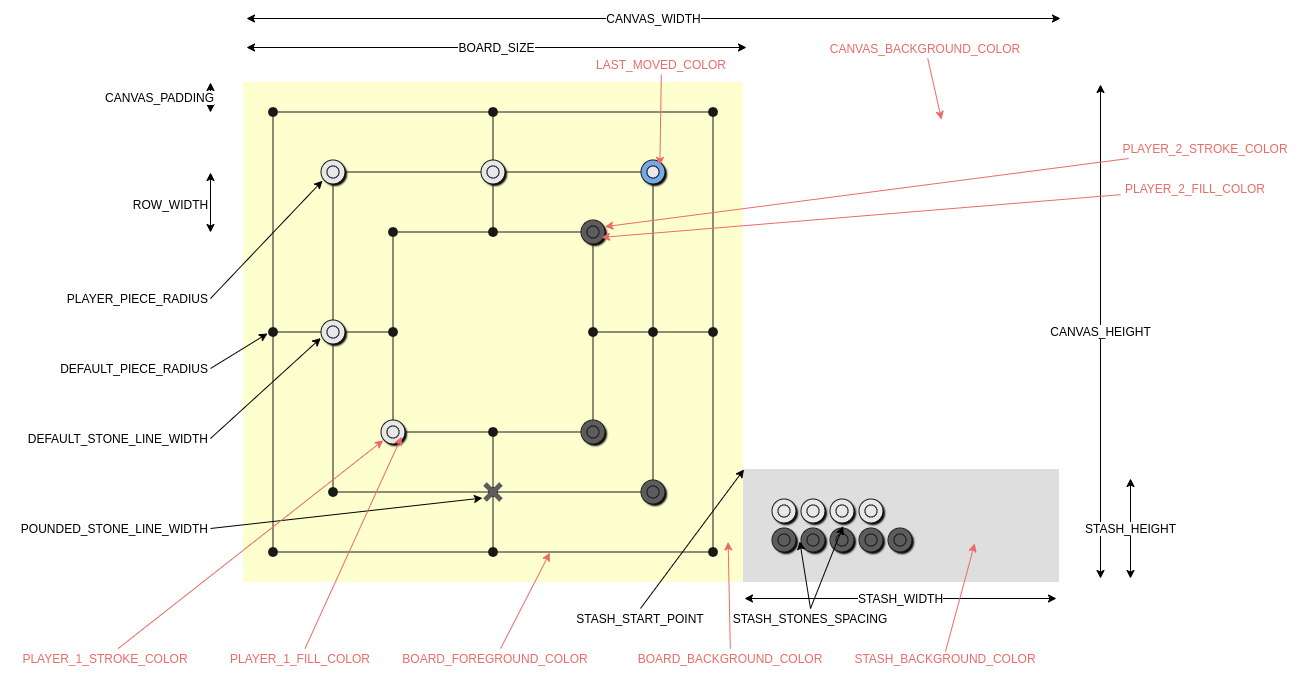
\includegraphics{../images/nmm-constants.png}

    \begin{tcolorbox}[breakable, size=fbox, boxrule=1pt, pad at break*=1mm,colback=cellbackground, colframe=cellborder]
\prompt{In}{incolor}{ }{\boxspacing}
\begin{Verbatim}[commandchars=\\\{\}]
\PY{n}{BOARD\PYZus{}SIZE} \PY{o}{=} \PY{l+m+mi}{500}
\PY{n}{CANVAS\PYZus{}PADDING} \PY{o}{=} \PY{l+m+mi}{30}
\PY{n}{ROW\PYZus{}WIDTH} \PY{o}{=} \PY{l+m+mi}{60}
\PY{n}{PLAYER\PYZus{}PIECE\PYZus{}RADIUS} \PY{o}{=} \PY{l+m+mi}{12}
\PY{n}{DEFAULT\PYZus{}PIECE\PYZus{}RADIUS} \PY{o}{=} \PY{l+m+mi}{5}

\PY{n}{DEFAULT\PYZus{}STONE\PYZus{}LINE\PYZus{}WIDTH} \PY{o}{=} \PY{l+m+mi}{1}
\PY{n}{SELECTED\PYZus{}STONE\PYZus{}LINE\PYZus{}WIDTH} \PY{o}{=} \PY{l+m+mi}{3}
\PY{n}{POUNDED\PYZus{}STONE\PYZus{}LINE\PYZus{}WIDTH} \PY{o}{=} \PY{l+m+mi}{5}

\PY{n}{STASH\PYZus{}STONES\PYZus{}SPACING} \PY{o}{=} \PY{l+m+mi}{5}

\PY{n}{STASH\PYZus{}HEIGHT} \PY{o}{=} \PY{p}{(}\PY{p}{(}\PY{n}{PLAYER\PYZus{}PIECE\PYZus{}RADIUS} \PY{o}{*} \PY{l+m+mi}{2} \PY{p}{)} \PY{o}{*} \PY{l+m+mi}{2}\PY{p}{)} \PY{o}{+} \PY{p}{(}\PY{n}{STASH\PYZus{}STONES\PYZus{}SPACING}\PY{p}{)} \PY{o}{+} \PY{p}{(}\PY{n}{CANVAS\PYZus{}PADDING} \PY{o}{*} \PY{l+m+mi}{2}\PY{p}{)}
\PY{n}{STASH\PYZus{}WIDTH} \PY{o}{=} \PY{p}{(}\PY{p}{(}\PY{n}{PLAYER\PYZus{}PIECE\PYZus{}RADIUS} \PY{o}{*} \PY{l+m+mi}{2} \PY{p}{)} \PY{o}{*} \PY{l+m+mi}{9}\PY{p}{)} \PY{o}{+} \PY{p}{(}\PY{n}{STASH\PYZus{}STONES\PYZus{}SPACING} \PY{o}{*} \PY{l+m+mi}{8}\PY{p}{)} \PY{o}{+} \PY{p}{(}\PY{n}{CANVAS\PYZus{}PADDING} \PY{o}{*} \PY{l+m+mi}{2}\PY{p}{)}

\PY{n}{CANVAS\PYZus{}HEIGHT} \PY{o}{=} \PY{n}{BOARD\PYZus{}SIZE}
\PY{n}{CANVAS\PYZus{}WIDTH} \PY{o}{=} \PY{l+m+mi}{1500}

\PY{n}{STASH\PYZus{}STARTING\PYZus{}POINT\PYZus{}X} \PY{o}{=} \PY{n}{BOARD\PYZus{}SIZE}
\PY{n}{STASH\PYZus{}STARTING\PYZus{}POINT\PYZus{}Y} \PY{o}{=} \PY{n}{CANVAS\PYZus{}HEIGHT} \PY{o}{\PYZhy{}} \PY{n}{STASH\PYZus{}HEIGHT}
\end{Verbatim}
\end{tcolorbox}

    \hypertarget{farben}{%
\subsubsection{Farben}\label{farben}}

Die Farben für das Spiel werden im Folgenden definiert. In der obigen
Abbildung sind diese genauer erklärt.

    \begin{tcolorbox}[breakable, size=fbox, boxrule=1pt, pad at break*=1mm,colback=cellbackground, colframe=cellborder]
\prompt{In}{incolor}{ }{\boxspacing}
\begin{Verbatim}[commandchars=\\\{\}]
\PY{n}{CANVAS\PYZus{}BACKGROUND\PYZus{}COLOR} \PY{o}{=} \PY{l+s+s1}{\PYZsq{}}\PY{l+s+s1}{\PYZsh{}ffffff}\PY{l+s+s1}{\PYZsq{}}
\PY{n}{BOARD\PYZus{}FOREGROUND\PYZus{}COLOR} \PY{o}{=} \PY{l+s+s1}{\PYZsq{}}\PY{l+s+s1}{\PYZsh{}191919}\PY{l+s+s1}{\PYZsq{}}
\PY{n}{BOARD\PYZus{}BACKGROUND\PYZus{}COLOR} \PY{o}{=} \PY{l+s+s1}{\PYZsq{}}\PY{l+s+s1}{\PYZsh{}ffffcb}\PY{l+s+s1}{\PYZsq{}}
\PY{n}{STASH\PYZus{}BACKGROUND\PYZus{}COLOR} \PY{o}{=} \PY{l+s+s1}{\PYZsq{}}\PY{l+s+s1}{\PYZsh{}dedede}\PY{l+s+s1}{\PYZsq{}}
\PY{n}{PLAYER\PYZus{}1\PYZus{}FILL\PYZus{}COLOR} \PY{o}{=} \PY{l+s+s1}{\PYZsq{}}\PY{l+s+s1}{\PYZsh{}E8E8E8}\PY{l+s+s1}{\PYZsq{}}
\PY{n}{PLAYER\PYZus{}1\PYZus{}STROKE\PYZus{}COLOR} \PY{o}{=} \PY{l+s+s1}{\PYZsq{}}\PY{l+s+s1}{\PYZsh{}191919}\PY{l+s+s1}{\PYZsq{}}
\PY{n}{PLAYER\PYZus{}2\PYZus{}FILL\PYZus{}COLOR} \PY{o}{=} \PY{l+s+s1}{\PYZsq{}}\PY{l+s+s1}{\PYZsh{}5c5c5c}\PY{l+s+s1}{\PYZsq{}}
\PY{n}{PLAYER\PYZus{}2\PYZus{}STROKE\PYZus{}COLOR} \PY{o}{=} \PY{l+s+s1}{\PYZsq{}}\PY{l+s+s1}{\PYZsh{}191919}\PY{l+s+s1}{\PYZsq{}}
\PY{n}{LAST\PYZus{}MOVED\PYZus{}COLOR} \PY{o}{=} \PY{l+s+s1}{\PYZsq{}}\PY{l+s+s1}{\PYZsh{}61aced}\PY{l+s+s1}{\PYZsq{}}
\end{Verbatim}
\end{tcolorbox}

    \hypertarget{text}{%
\subsubsection{Text}\label{text}}

In der GUI gibt es drei verschiedene Textarten:
\begin{itemize}
    \item Spielnachricht (wer spielt gerade oder ob das Spiel beendet ist),
    \item Hinweise (falls zum Beispiel eine ungültige Aktion ausgeführt worden ist) und - Informationen über den letzten Zug der künstlichen Intelligenz.
\end{itemize}

Diese Textarten haben eine eigene Schriftart, -größe und -farbe.

    \begin{tcolorbox}[breakable, size=fbox, boxrule=1pt, pad at break*=1mm,colback=cellbackground, colframe=cellborder]
\prompt{In}{incolor}{ }{\boxspacing}
\begin{Verbatim}[commandchars=\\\{\}]
\PY{n}{TEXT\PYZus{}X} \PY{o}{=} \PY{n}{BOARD\PYZus{}SIZE} \PY{o}{+} \PY{n}{CANVAS\PYZus{}PADDING}
\PY{n}{TEXT\PYZus{}Y} \PY{o}{=} \PY{n}{CANVAS\PYZus{}PADDING}
\PY{n}{TEXT\PYZus{}MAX\PYZus{}WIDTH} \PY{o}{=} \PY{n}{CANVAS\PYZus{}WIDTH} \PY{o}{\PYZhy{}} \PY{n}{BOARD\PYZus{}SIZE} \PY{o}{\PYZhy{}} \PY{l+m+mi}{2} \PY{o}{*} \PY{n}{CANVAS\PYZus{}PADDING}
\PY{n}{TEXT\PYZus{}VERTICAL\PYZus{}PADDING} \PY{o}{=} \PY{l+m+mi}{30}
\PY{n}{TEXT\PYZus{}MSG\PYZus{}FONT} \PY{o}{=} \PY{l+s+s1}{\PYZsq{}}\PY{l+s+s1}{18px sans\PYZhy{}serif}\PY{l+s+s1}{\PYZsq{}}
\PY{n}{TEXT\PYZus{}MSG\PYZus{}COLOR} \PY{o}{=} \PY{l+s+s1}{\PYZsq{}}\PY{l+s+s1}{\PYZsh{}333333}\PY{l+s+s1}{\PYZsq{}}
\PY{n}{TEXT\PYZus{}HINT\PYZus{}FONT} \PY{o}{=} \PY{l+s+s1}{\PYZsq{}}\PY{l+s+s1}{14px sans\PYZhy{}serif}\PY{l+s+s1}{\PYZsq{}}
\PY{n}{TEXT\PYZus{}HINT\PYZus{}COLOR} \PY{o}{=} \PY{l+s+s1}{\PYZsq{}}\PY{l+s+s1}{\PYZsh{}c75528}\PY{l+s+s1}{\PYZsq{}}
\PY{n}{TEXT\PYZus{}INFO\PYZus{}FONT} \PY{o}{=} \PY{l+s+s1}{\PYZsq{}}\PY{l+s+s1}{14px mono}\PY{l+s+s1}{\PYZsq{}}
\PY{n}{TEXT\PYZus{}INFO\PYZus{}COLOR} \PY{o}{=} \PY{l+s+s1}{\PYZsq{}}\PY{l+s+s1}{\PYZsh{}333333}\PY{l+s+s1}{\PYZsq{}}
\end{Verbatim}
\end{tcolorbox}

    \hypertarget{schatten}{%
\subsubsection{Schatten}\label{schatten}}

Um das Spiel dynamischer zu gestalten, haben Spielsteine einen Schatten.

    \begin{tcolorbox}[breakable, size=fbox, boxrule=1pt, pad at break*=1mm,colback=cellbackground, colframe=cellborder]
\prompt{In}{incolor}{ }{\boxspacing}
\begin{Verbatim}[commandchars=\\\{\}]
\PY{n}{SHADOW\PYZus{}COLOR\PYZus{}ENABLED} \PY{o}{=} \PY{l+s+s1}{\PYZsq{}}\PY{l+s+s1}{\PYZsh{}000000}\PY{l+s+s1}{\PYZsq{}}
\PY{n}{SHADOW\PYZus{}OFFSET\PYZus{}X\PYZus{}ENABLED} \PY{o}{=} \PY{l+m+mi}{2}
\PY{n}{SHADOW\PYZus{}OFFSET\PYZus{}Y\PYZus{}ENABLED} \PY{o}{=} \PY{l+m+mi}{2}
\PY{n}{SHADOW\PYZus{}BLUR\PYZus{}ENABLED} \PY{o}{=} \PY{l+m+mi}{2}

\PY{n}{SHADOW\PYZus{}COLOR\PYZus{}DISABLED} \PY{o}{=} \PY{l+s+s1}{\PYZsq{}}\PY{l+s+s1}{rgba(0, 0, 0, 0)}\PY{l+s+s1}{\PYZsq{}}
\PY{n}{SHADOW\PYZus{}OFFSET\PYZus{}X\PYZus{}DISABLED} \PY{o}{=} \PY{l+m+mi}{0}
\PY{n}{SHADOW\PYZus{}OFFSET\PYZus{}Y\PYZus{}DISABLED} \PY{o}{=} \PY{l+m+mi}{0}
\PY{n}{SHADOW\PYZus{}BLUR\PYZus{}DISABLED} \PY{o}{=} \PY{l+m+mi}{0}
\end{Verbatim}
\end{tcolorbox}

    \hypertarget{berechnete-werte}{%
\subsubsection{Berechnete Werte}\label{berechnete-werte}}

Die Koordinaten für die Knoten lassen sich aus den obrigen Konstanten
berechnen. Da das Mühlespielbrett horizontal und vertikal identisch ist,
werden für die Koordinaten auf der x- und y-Achse die gleichen Werte
benötigt, die mit \(av\) (für \emph{available values}) bezeichnet
werden. Es werden insgesamt sieben Werte \(av_0\) bis \(av_6\) benötigt,
die in der folgenden Abbildung dargestellt werden.

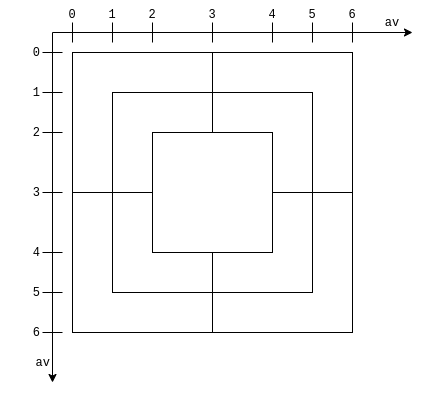
\includegraphics{../images/nmm-av.png}

Die Werte lassen sich wie folgt berechnen.

\[ av_0 =  CANVAS\_PADDING \] \[ av_1 =  CANVAS\_PADDING + ROW\_WIDTH \]
\[ av_2 =  CANVAS\_PADDING + 2 \cdot ROW\_WIDTH \]
\[ av_3 =  \frac{BOARD\_SIZE}{2}\]
\[ av_4 =  BOARD\_SIZE - (CANVAS\_PADDING + 2 \cdot ROW\_WIDTH) \]
\[ av_5 =  BOARD\_SIZE - (CANVAS\_PADDING + ROW\_WIDTH)\]
\[ av_6 =  BOARD\_SIZE - CANVAS\_PADDING \]

    \begin{tcolorbox}[breakable, size=fbox, boxrule=1pt, pad at break*=1mm,colback=cellbackground, colframe=cellborder]
\prompt{In}{incolor}{ }{\boxspacing}
\begin{Verbatim}[commandchars=\\\{\}]
\PY{n}{av} \PY{o}{=} \PY{p}{(}
    \PY{n}{math}\PY{o}{.}\PY{n}{floor}\PY{p}{(}\PY{n}{CANVAS\PYZus{}PADDING}\PY{p}{)}\PY{p}{,}
    \PY{n}{math}\PY{o}{.}\PY{n}{floor}\PY{p}{(}\PY{n}{CANVAS\PYZus{}PADDING} \PY{o}{+} \PY{n}{ROW\PYZus{}WIDTH}\PY{p}{)}\PY{p}{,}
    \PY{n}{math}\PY{o}{.}\PY{n}{floor}\PY{p}{(}\PY{n}{CANVAS\PYZus{}PADDING} \PY{o}{+} \PY{l+m+mi}{2} \PY{o}{*} \PY{n}{ROW\PYZus{}WIDTH}\PY{p}{)}\PY{p}{,}
    \PY{n}{math}\PY{o}{.}\PY{n}{floor}\PY{p}{(}\PY{n}{BOARD\PYZus{}SIZE} \PY{o}{/} \PY{l+m+mi}{2}\PY{p}{)}\PY{p}{,}
    \PY{n}{math}\PY{o}{.}\PY{n}{floor}\PY{p}{(}\PY{n}{BOARD\PYZus{}SIZE} \PY{o}{\PYZhy{}} \PY{p}{(}\PY{n}{CANVAS\PYZus{}PADDING} \PY{o}{+} \PY{l+m+mi}{2} \PY{o}{*} \PY{n}{ROW\PYZus{}WIDTH}\PY{p}{)}\PY{p}{)}\PY{p}{,}
    \PY{n}{math}\PY{o}{.}\PY{n}{floor}\PY{p}{(}\PY{n}{BOARD\PYZus{}SIZE} \PY{o}{\PYZhy{}} \PY{p}{(}\PY{n}{CANVAS\PYZus{}PADDING} \PY{o}{+} \PY{n}{ROW\PYZus{}WIDTH}\PY{p}{)}\PY{p}{)}\PY{p}{,}
    \PY{n}{math}\PY{o}{.}\PY{n}{floor}\PY{p}{(}\PY{n}{BOARD\PYZus{}SIZE} \PY{o}{\PYZhy{}} \PY{n}{CANVAS\PYZus{}PADDING}\PY{p}{)}
\PY{p}{)}
\end{Verbatim}
\end{tcolorbox}

    \hypertarget{koordinaten}{%
\subsubsection{Koordinaten}\label{koordinaten}}

Die Koordinaten der Knoten sind in dem zweidimensionalen Tupel
\texttt{coords} definiert. Zuerst wird der Ring definiert, von außen
nach innen. Danach die Position im Ring, beginnend von oben links und
dann im Uhrzeigersinn. In der Abbildung sind die Knoten mit den
Koordinaten dargestellt. Die Werte von den Koordinaten sind die x- und
y-Werte auf der Zeichenfläche, definiert in \texttt{av}.

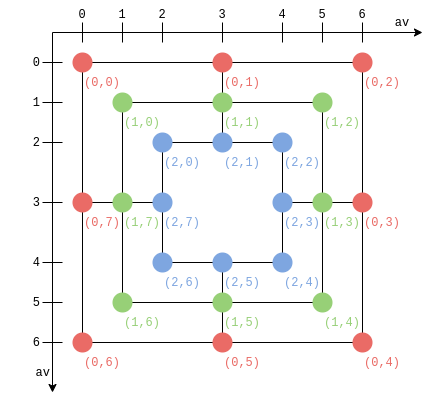
\includegraphics{../images/nmm-coords.png}

    \begin{tcolorbox}[breakable, size=fbox, boxrule=1pt, pad at break*=1mm,colback=cellbackground, colframe=cellborder]
\prompt{In}{incolor}{ }{\boxspacing}
\begin{Verbatim}[commandchars=\\\{\}]
\PY{n}{coords} \PY{o}{=} \PY{p}{(}
    \PY{p}{(}
        \PY{p}{(}\PY{n}{av}\PY{p}{[}\PY{l+m+mi}{0}\PY{p}{]}\PY{p}{,} \PY{n}{av}\PY{p}{[}\PY{l+m+mi}{0}\PY{p}{]}\PY{p}{)}\PY{p}{,}
        \PY{p}{(}\PY{n}{av}\PY{p}{[}\PY{l+m+mi}{3}\PY{p}{]}\PY{p}{,} \PY{n}{av}\PY{p}{[}\PY{l+m+mi}{0}\PY{p}{]}\PY{p}{)}\PY{p}{,}
        \PY{p}{(}\PY{n}{av}\PY{p}{[}\PY{l+m+mi}{6}\PY{p}{]}\PY{p}{,} \PY{n}{av}\PY{p}{[}\PY{l+m+mi}{0}\PY{p}{]}\PY{p}{)}\PY{p}{,}
        \PY{p}{(}\PY{n}{av}\PY{p}{[}\PY{l+m+mi}{6}\PY{p}{]}\PY{p}{,} \PY{n}{av}\PY{p}{[}\PY{l+m+mi}{3}\PY{p}{]}\PY{p}{)}\PY{p}{,}
        \PY{p}{(}\PY{n}{av}\PY{p}{[}\PY{l+m+mi}{6}\PY{p}{]}\PY{p}{,} \PY{n}{av}\PY{p}{[}\PY{l+m+mi}{6}\PY{p}{]}\PY{p}{)}\PY{p}{,}
        \PY{p}{(}\PY{n}{av}\PY{p}{[}\PY{l+m+mi}{3}\PY{p}{]}\PY{p}{,} \PY{n}{av}\PY{p}{[}\PY{l+m+mi}{6}\PY{p}{]}\PY{p}{)}\PY{p}{,}
        \PY{p}{(}\PY{n}{av}\PY{p}{[}\PY{l+m+mi}{0}\PY{p}{]}\PY{p}{,} \PY{n}{av}\PY{p}{[}\PY{l+m+mi}{6}\PY{p}{]}\PY{p}{)}\PY{p}{,}
        \PY{p}{(}\PY{n}{av}\PY{p}{[}\PY{l+m+mi}{0}\PY{p}{]}\PY{p}{,} \PY{n}{av}\PY{p}{[}\PY{l+m+mi}{3}\PY{p}{]}\PY{p}{)}
    \PY{p}{)}\PY{p}{,}
    \PY{p}{(}
        \PY{p}{(}\PY{n}{av}\PY{p}{[}\PY{l+m+mi}{1}\PY{p}{]}\PY{p}{,} \PY{n}{av}\PY{p}{[}\PY{l+m+mi}{1}\PY{p}{]}\PY{p}{)}\PY{p}{,}
        \PY{p}{(}\PY{n}{av}\PY{p}{[}\PY{l+m+mi}{3}\PY{p}{]}\PY{p}{,} \PY{n}{av}\PY{p}{[}\PY{l+m+mi}{1}\PY{p}{]}\PY{p}{)}\PY{p}{,}
        \PY{p}{(}\PY{n}{av}\PY{p}{[}\PY{l+m+mi}{5}\PY{p}{]}\PY{p}{,} \PY{n}{av}\PY{p}{[}\PY{l+m+mi}{1}\PY{p}{]}\PY{p}{)}\PY{p}{,}
        \PY{p}{(}\PY{n}{av}\PY{p}{[}\PY{l+m+mi}{5}\PY{p}{]}\PY{p}{,} \PY{n}{av}\PY{p}{[}\PY{l+m+mi}{3}\PY{p}{]}\PY{p}{)}\PY{p}{,}
        \PY{p}{(}\PY{n}{av}\PY{p}{[}\PY{l+m+mi}{5}\PY{p}{]}\PY{p}{,} \PY{n}{av}\PY{p}{[}\PY{l+m+mi}{5}\PY{p}{]}\PY{p}{)}\PY{p}{,}
        \PY{p}{(}\PY{n}{av}\PY{p}{[}\PY{l+m+mi}{3}\PY{p}{]}\PY{p}{,} \PY{n}{av}\PY{p}{[}\PY{l+m+mi}{5}\PY{p}{]}\PY{p}{)}\PY{p}{,}
        \PY{p}{(}\PY{n}{av}\PY{p}{[}\PY{l+m+mi}{1}\PY{p}{]}\PY{p}{,} \PY{n}{av}\PY{p}{[}\PY{l+m+mi}{5}\PY{p}{]}\PY{p}{)}\PY{p}{,}
        \PY{p}{(}\PY{n}{av}\PY{p}{[}\PY{l+m+mi}{1}\PY{p}{]}\PY{p}{,} \PY{n}{av}\PY{p}{[}\PY{l+m+mi}{3}\PY{p}{]}\PY{p}{)}
    \PY{p}{)}\PY{p}{,}
    \PY{p}{(}
        \PY{p}{(}\PY{n}{av}\PY{p}{[}\PY{l+m+mi}{2}\PY{p}{]}\PY{p}{,} \PY{n}{av}\PY{p}{[}\PY{l+m+mi}{2}\PY{p}{]}\PY{p}{)}\PY{p}{,}
        \PY{p}{(}\PY{n}{av}\PY{p}{[}\PY{l+m+mi}{3}\PY{p}{]}\PY{p}{,} \PY{n}{av}\PY{p}{[}\PY{l+m+mi}{2}\PY{p}{]}\PY{p}{)}\PY{p}{,}
        \PY{p}{(}\PY{n}{av}\PY{p}{[}\PY{l+m+mi}{4}\PY{p}{]}\PY{p}{,} \PY{n}{av}\PY{p}{[}\PY{l+m+mi}{2}\PY{p}{]}\PY{p}{)}\PY{p}{,}
        \PY{p}{(}\PY{n}{av}\PY{p}{[}\PY{l+m+mi}{4}\PY{p}{]}\PY{p}{,} \PY{n}{av}\PY{p}{[}\PY{l+m+mi}{3}\PY{p}{]}\PY{p}{)}\PY{p}{,}
        \PY{p}{(}\PY{n}{av}\PY{p}{[}\PY{l+m+mi}{4}\PY{p}{]}\PY{p}{,} \PY{n}{av}\PY{p}{[}\PY{l+m+mi}{4}\PY{p}{]}\PY{p}{)}\PY{p}{,}
        \PY{p}{(}\PY{n}{av}\PY{p}{[}\PY{l+m+mi}{3}\PY{p}{]}\PY{p}{,} \PY{n}{av}\PY{p}{[}\PY{l+m+mi}{4}\PY{p}{]}\PY{p}{)}\PY{p}{,}
        \PY{p}{(}\PY{n}{av}\PY{p}{[}\PY{l+m+mi}{2}\PY{p}{]}\PY{p}{,} \PY{n}{av}\PY{p}{[}\PY{l+m+mi}{4}\PY{p}{]}\PY{p}{)}\PY{p}{,}
        \PY{p}{(}\PY{n}{av}\PY{p}{[}\PY{l+m+mi}{2}\PY{p}{]}\PY{p}{,} \PY{n}{av}\PY{p}{[}\PY{l+m+mi}{3}\PY{p}{]}\PY{p}{)}
    \PY{p}{)}
\PY{p}{)} 
\end{Verbatim}
\end{tcolorbox}

    \hypertarget{funktionen-zum-zeichnen}{%
\subsection{Funktionen zum Zeichnen}\label{funktionen-zum-zeichnen}}

Die grafische Oberfläche (englisch \emph{graphical user interface}, GUI)
wird mit dem Python-Modul ipycanvas aufgebaut. Dieses Modul ermöglicht
die Verwendung einer interaktiven Zeichenfläche zum Zeichnen von
2D-Objekten in IPython. Es bringt eine Reihe von Funktionen mit, um
einfache Formen zeichnen zu können. Gezeichnet wird auf einem
2D-Canvas-Objekt mit den Startkoordinaten \texttt{(0,0)} oben links.

    \begin{tcolorbox}[breakable, size=fbox, boxrule=1pt, pad at break*=1mm,colback=cellbackground, colframe=cellborder]
\prompt{In}{incolor}{ }{\boxspacing}
\begin{Verbatim}[commandchars=\\\{\}]
\PY{k+kn}{import} \PY{n+nn}{ipycanvas}
\end{Verbatim}
\end{tcolorbox}

    Die Funktion \texttt{toggleShadow} schaltet den Schatten auf einem
gegebenen Canvas ein und aus. Sie hat folgende Eingabeparameter:

\begin{itemize}
\tightlist
\item
  \texttt{c} ist eine Referenz auf ein Canvas-Objekt.
\item
  \texttt{enable} ist ein boolischer Wert, der angibt, ob Schatten auf
  dem Canvas \texttt{c} ein oder ausgeschaltet werden soll.
\end{itemize}

Wird der Schatten eingeschaltet, werden die Schatteneigenschaften des
Canvas mit den oben definierten Konstanten gesetzt. Andernfalls werden
die Standardwerte von \emph{ipycanvas} gesetzt, was bedeutet, der
Schatten wird deaktiviert.

    \begin{tcolorbox}[breakable, size=fbox, boxrule=1pt, pad at break*=1mm,colback=cellbackground, colframe=cellborder]
\prompt{In}{incolor}{ }{\boxspacing}
\begin{Verbatim}[commandchars=\\\{\}]
\PY{k}{def} \PY{n+nf}{toggleShadow}\PY{p}{(}\PY{n}{c}\PY{p}{,} \PY{n}{enable}\PY{p}{)}\PY{p}{:}
    \PY{n}{c}\PY{o}{.}\PY{n}{shadow\PYZus{}color}    \PY{o}{=} \PY{n}{SHADOW\PYZus{}COLOR\PYZus{}ENABLED}    \PY{k}{if} \PY{n}{enable} \PY{k}{else} \PY{n}{SHADOW\PYZus{}COLOR\PYZus{}DISABLED}
    \PY{n}{c}\PY{o}{.}\PY{n}{shadow\PYZus{}offset\PYZus{}x} \PY{o}{=} \PY{n}{SHADOW\PYZus{}OFFSET\PYZus{}X\PYZus{}ENABLED} \PY{k}{if} \PY{n}{enable} \PY{k}{else} \PY{n}{SHADOW\PYZus{}OFFSET\PYZus{}X\PYZus{}DISABLED}
    \PY{n}{c}\PY{o}{.}\PY{n}{shadow\PYZus{}offset\PYZus{}y} \PY{o}{=} \PY{n}{SHADOW\PYZus{}OFFSET\PYZus{}Y\PYZus{}ENABLED} \PY{k}{if} \PY{n}{enable} \PY{k}{else} \PY{n}{SHADOW\PYZus{}OFFSET\PYZus{}Y\PYZus{}DISABLED}
    \PY{n}{c}\PY{o}{.}\PY{n}{shadow\PYZus{}blur}     \PY{o}{=} \PY{n}{SHADOW\PYZus{}BLUR\PYZus{}ENABLED}     \PY{k}{if} \PY{n}{enable} \PY{k}{else} \PY{n}{SHADOW\PYZus{}BLUR\PYZus{}DISABLED}
\end{Verbatim}
\end{tcolorbox}

    Die Funktion \texttt{drawCircle} dient zum Zeichnen eines Kreises auf
einem Zeichenfeld. Die Funktion hat vier Argumente und drei optionale
Parameter:

\begin{itemize}
\tightlist
\item
  \texttt{c} ist eine Referenz auf ein Canvas-Objekt, auf dem der Kreis
  gezeichnet werden soll.
\item
  \texttt{coords} ist die Koordinate des Mittelpunktes des Kreies.
\item
  \texttt{radius} ist der Radius des Kreises.
\item
  \texttt{color} gibt die Farbe des Kreises an.
\item
  \texttt{strokeColor} ist ein optionaler Parameter, der die Farbe der
  Umrandung angibt. Der Standardwert ist \texttt{None}. In dem Fall wird
  der Kreis nicht umrandet.
\item
  \texttt{lineWidth} ist ein optionaler Parameter, der die Liniendicke
  angibt. Der Standardwert ist in der Kontante
  \texttt{DEFAULT\_STONE\_LINE\_WIDTH} definiert.
\item
  \texttt{useShadow} ist ein optionaler, boolischer Wert. Wenn er
  gesetzt ist, wird ein Schatten von dem Kreis gemalt. Standardmäßig ist
  der Wert \texttt{False}.
\end{itemize}

    \begin{tcolorbox}[breakable, size=fbox, boxrule=1pt, pad at break*=1mm,colback=cellbackground, colframe=cellborder]
\prompt{In}{incolor}{ }{\boxspacing}
\begin{Verbatim}[commandchars=\\\{\}]
\PY{k}{def} \PY{n+nf}{drawCircle}\PY{p}{(}
        \PY{n}{c}\PY{p}{,}
        \PY{n}{coords}\PY{p}{,}
        \PY{n}{radius}\PY{p}{,}
        \PY{n}{color}\PY{p}{,}
        \PY{n}{strokeColor} \PY{o}{=} \PY{k+kc}{None}\PY{p}{,}
        \PY{n}{lineWidth} \PY{o}{=} \PY{n}{DEFAULT\PYZus{}STONE\PYZus{}LINE\PYZus{}WIDTH}\PY{p}{,}
        \PY{n}{useShadow} \PY{o}{=} \PY{k+kc}{False}\PY{p}{)}\PY{p}{:}
    \PY{k}{if} \PY{n}{useShadow}\PY{p}{:}
        \PY{n}{toggleShadow}\PY{p}{(}\PY{n}{c}\PY{p}{,} \PY{k+kc}{True}\PY{p}{)}
    \PY{n}{c}\PY{o}{.}\PY{n}{fill\PYZus{}style} \PY{o}{=} \PY{n}{color}
    \PY{n}{c}\PY{o}{.}\PY{n}{fill\PYZus{}arc}\PY{p}{(}\PY{n}{coords}\PY{p}{[}\PY{l+m+mi}{0}\PY{p}{]}\PY{p}{,} \PY{n}{coords}\PY{p}{[}\PY{l+m+mi}{1}\PY{p}{]}\PY{p}{,} \PY{n}{radius}\PY{p}{,} \PY{l+m+mi}{0}\PY{p}{,} \PY{l+m+mi}{2} \PY{o}{*} \PY{n}{math}\PY{o}{.}\PY{n}{pi}\PY{p}{)}
    \PY{k}{if} \PY{n}{useShadow}\PY{p}{:}
        \PY{n}{toggleShadow}\PY{p}{(}\PY{n}{c}\PY{p}{,} \PY{k+kc}{False}\PY{p}{)}
    \PY{k}{if} \PY{n}{strokeColor} \PY{o+ow}{is} \PY{o+ow}{not} \PY{k+kc}{None}\PY{p}{:}
        \PY{n}{c}\PY{o}{.}\PY{n}{line\PYZus{}width} \PY{o}{=} \PY{n}{lineWidth}
        \PY{n}{c}\PY{o}{.}\PY{n}{stroke\PYZus{}style} \PY{o}{=} \PY{n}{strokeColor}
        \PY{n}{c}\PY{o}{.}\PY{n}{stroke\PYZus{}arc}\PY{p}{(}\PY{n}{coords}\PY{p}{[}\PY{l+m+mi}{0}\PY{p}{]}\PY{p}{,} \PY{n}{coords}\PY{p}{[}\PY{l+m+mi}{1}\PY{p}{]}\PY{p}{,} \PY{n}{radius}\PY{p}{,} \PY{l+m+mi}{0}\PY{p}{,} \PY{l+m+mi}{2} \PY{o}{*} \PY{n}{math}\PY{o}{.}\PY{n}{pi}\PY{p}{)}
\end{Verbatim}
\end{tcolorbox}

    Die Funktion \texttt{drawStone} dient zum Zeichnen eines Steines auf
einem Zeichenfeld mit Hilfe der Funktion \texttt{drawCircle}. Ein
Spielstein besteht aus zwei Kreisen und ein leerer Knoten (also wo sich
kein Spieler befinden) aus einem Kreis.

Die Funktion hat drei Argumente und zwei optionale Parameter:

\begin{itemize}
\tightlist
\item
  \texttt{c} ist eine Referenz auf ein Canvas-Objekt, auf dem der Stein
  gezeichnet werden soll;
\item
  \texttt{coords} ist die Koordinate des Mittelpunktes des Steines;
\item
  \texttt{player} gibt den Spieler an;
\item
  \texttt{selected} ist ein optionaler, boolischer Wert, der angibt, ob
  ein Spielerstein ausgewählt ist oder nicht. Der Standardwert ist
  \texttt{False};
\item
  \texttt{lastMoved} ist ein optionaler, boolischer Wert, der angibt ob
  der zu zeichnende Spielerstein zuletzt bewegt worden ist. Der
  Standardwert ist \texttt{False}.
\end{itemize}

    \begin{tcolorbox}[breakable, size=fbox, boxrule=1pt, pad at break*=1mm,colback=cellbackground, colframe=cellborder]
\prompt{In}{incolor}{ }{\boxspacing}
\begin{Verbatim}[commandchars=\\\{\}]
\PY{k}{def} \PY{n+nf}{drawStone}\PY{p}{(}\PY{n}{c}\PY{p}{,} \PY{n}{coords}\PY{p}{,} \PY{n}{player}\PY{p}{,} \PY{n}{selected} \PY{o}{=} \PY{k+kc}{False}\PY{p}{,} \PY{n}{lastMoved} \PY{o}{=} \PY{k+kc}{False}\PY{p}{)}\PY{p}{:}
    \PY{k}{if} \PY{n}{player} \PY{o}{==} \PY{n}{NO\PYZus{}PLAYER}\PY{p}{:}
        \PY{n}{drawCircle}\PY{p}{(}\PY{n}{c}\PY{p}{,} \PY{n}{coords}\PY{p}{,} \PY{n}{DEFAULT\PYZus{}PIECE\PYZus{}RADIUS}\PY{p}{,} \PY{n}{BOARD\PYZus{}FOREGROUND\PYZus{}COLOR}\PY{p}{)}
    \PY{k}{else}\PY{p}{:}
        \PY{n}{color}       \PY{o}{=} \PY{n}{PLAYER\PYZus{}1\PYZus{}FILL\PYZus{}COLOR}   \PY{k}{if} \PY{n}{player} \PY{o}{==} \PY{n}{PLAYER\PYZus{}1} \PY{k}{else} \PY{n}{PLAYER\PYZus{}2\PYZus{}FILL\PYZus{}COLOR}
        \PY{n}{strokeColor} \PY{o}{=} \PY{n}{PLAYER\PYZus{}1\PYZus{}STROKE\PYZus{}COLOR} \PY{k}{if} \PY{n}{player} \PY{o}{==} \PY{n}{PLAYER\PYZus{}1} \PY{k}{else} \PY{n}{PLAYER\PYZus{}2\PYZus{}STROKE\PYZus{}COLOR}
        
        \PY{n}{lineWidth} \PY{o}{=} \PY{n}{SELECTED\PYZus{}STONE\PYZus{}LINE\PYZus{}WIDTH} \PY{k}{if} \PY{n}{selected} \PY{k}{else} \PY{n}{DEFAULT\PYZus{}STONE\PYZus{}LINE\PYZus{}WIDTH}
        \PY{n}{drawCircle}\PY{p}{(}
            \PY{n}{c}\PY{p}{,}
            \PY{n}{coords}\PY{p}{,}
            \PY{n}{PLAYER\PYZus{}PIECE\PYZus{}RADIUS}\PY{p}{,}
            \PY{n}{LAST\PYZus{}MOVED\PYZus{}COLOR} \PY{k}{if} \PY{n}{lastMoved} \PY{k}{else} \PY{n}{color}\PY{p}{,}
            \PY{n}{strokeColor}\PY{p}{,}
            \PY{n}{lineWidth}\PY{p}{,}
            \PY{n}{useShadow} \PY{o}{=} \PY{k+kc}{True}\PY{p}{)}
        \PY{n}{drawCircle}\PY{p}{(}
            \PY{n}{c}\PY{p}{,}
            \PY{n}{coords}\PY{p}{,}
            \PY{n}{math}\PY{o}{.}\PY{n}{floor}\PY{p}{(}\PY{n}{PLAYER\PYZus{}PIECE\PYZus{}RADIUS} \PY{o}{/} \PY{l+m+mi}{2}\PY{p}{)}\PY{p}{,}
            \PY{n}{color}\PY{p}{,}
            \PY{n}{strokeColor}\PY{p}{,}
            \PY{n}{lineWidth}\PY{p}{)}
\end{Verbatim}
\end{tcolorbox}

    Die Funktion \texttt{drawPoundedStone} dient zum Zeichnen eines
geschlagenden Steines auf einem Zeichenfeld. Ein geschlagender Stein
wird durch ein Kreuz in der GUI dargestellt.

Die Funktion hat drei Argumente:

\begin{itemize}
\tightlist
\item
  \texttt{c} ist eine Referenz auf ein Canvas-Objekt, auf dem der
  geschlagende Stein gezeichnet werden soll;
\item
  \texttt{coords} ist die Koordinate des Mittelpunktes des geschlagenden
  Steines;
\item
  \texttt{player} gibt den Spieler des Steines an.
\end{itemize}

    \begin{tcolorbox}[breakable, size=fbox, boxrule=1pt, pad at break*=1mm,colback=cellbackground, colframe=cellborder]
\prompt{In}{incolor}{ }{\boxspacing}
\begin{Verbatim}[commandchars=\\\{\}]
\PY{k}{def} \PY{n+nf}{drawPoundedStone}\PY{p}{(}\PY{n}{c}\PY{p}{,} \PY{n}{coords}\PY{p}{,} \PY{n}{player}\PY{p}{)}\PY{p}{:}
    \PY{n}{x}\PY{p}{,} \PY{n}{y} \PY{o}{=} \PY{n}{coords}
    \PY{n}{offset} \PY{o}{=} \PY{n+nb}{int}\PY{p}{(}\PY{n}{math}\PY{o}{.}\PY{n}{sin}\PY{p}{(}\PY{l+m+mf}{0.25}\PY{o}{*}\PY{n}{math}\PY{o}{.}\PY{n}{pi}\PY{p}{)} \PY{o}{*} \PY{n}{PLAYER\PYZus{}PIECE\PYZus{}RADIUS}\PY{p}{)}
    \PY{n}{c}\PY{o}{.}\PY{n}{line\PYZus{}width} \PY{o}{=} \PY{n}{POUNDED\PYZus{}STONE\PYZus{}LINE\PYZus{}WIDTH}
    \PY{n}{c}\PY{o}{.}\PY{n}{stroke\PYZus{}style} \PY{o}{=} \PY{n}{PLAYER\PYZus{}1\PYZus{}FILL\PYZus{}COLOR}   \PY{k}{if} \PY{n}{player} \PY{o}{==} \PY{n}{PLAYER\PYZus{}1} \PY{k}{else} \PY{n}{PLAYER\PYZus{}2\PYZus{}FILL\PYZus{}COLOR}
    \PY{k}{with} \PY{n}{ipycanvas}\PY{o}{.}\PY{n}{hold\PYZus{}canvas}\PY{p}{(}\PY{n}{c}\PY{p}{)}\PY{p}{:}
        \PY{n}{c}\PY{o}{.}\PY{n}{stroke\PYZus{}line}\PY{p}{(}\PY{n}{x} \PY{o}{\PYZhy{}} \PY{n}{offset}\PY{p}{,} \PY{n}{y} \PY{o}{\PYZhy{}} \PY{n}{offset}\PY{p}{,} \PY{n}{x} \PY{o}{+} \PY{n}{offset}\PY{p}{,} \PY{n}{y} \PY{o}{+} \PY{n}{offset}\PY{p}{)}
        \PY{n}{c}\PY{o}{.}\PY{n}{stroke\PYZus{}line}\PY{p}{(}\PY{n}{x} \PY{o}{\PYZhy{}} \PY{n}{offset}\PY{p}{,} \PY{n}{y} \PY{o}{+} \PY{n}{offset}\PY{p}{,} \PY{n}{x} \PY{o}{+} \PY{n}{offset}\PY{p}{,} \PY{n}{y} \PY{o}{\PYZhy{}} \PY{n}{offset}\PY{p}{)}
    
\end{Verbatim}
\end{tcolorbox}

    Die Funktion \texttt{drawText} zeichnet einen Text auf einer
Zeichenfläche. Die Funktion hat zwei Argumente und zwei optionale
Parameter:

\begin{itemize}
\tightlist
\item
  \texttt{c} ist eine Referenz auf ein Canvas-Objekt, auf dem der Text
  gezeichnet werden soll.
\item
  \texttt{msg} ist die Nachricht, die auf dem Canvas geschrieben werden
  soll.
\item
  \texttt{hint} ist ein optionaler String, der ein Hinweis oder eine
  Warnung ist. Standardmäßig ist die Variable auf \texttt{None} gesetzt.
\item
  \texttt{information} ist ein optionales Dictionary. Alle Einträge des
  Dictionaries werden als Information auf dem Zeichenfeld ausgegeben.
\end{itemize}

Bei jedem Funktionsaufruf wird am Anfang der Inhalt der Zeichenfläche
gelöscht, sodass sich immer nur eine Version der Texte auf der
Zeichenfläche befindet.

    \begin{tcolorbox}[breakable, size=fbox, boxrule=1pt, pad at break*=1mm,colback=cellbackground, colframe=cellborder]
\prompt{In}{incolor}{ }{\boxspacing}
\begin{Verbatim}[commandchars=\\\{\}]
\PY{k}{def} \PY{n+nf}{drawText}\PY{p}{(}\PY{n}{c}\PY{p}{,} \PY{n}{msg}\PY{p}{,} \PY{n}{hint} \PY{o}{=} \PY{k+kc}{None}\PY{p}{,} \PY{n}{information} \PY{o}{=} \PY{k+kc}{None}\PY{p}{)}\PY{p}{:}
    \PY{k}{with} \PY{n}{ipycanvas}\PY{o}{.}\PY{n}{hold\PYZus{}canvas}\PY{p}{(}\PY{n}{c}\PY{p}{)}\PY{p}{:}
        \PY{n}{c}\PY{o}{.}\PY{n}{clear}\PY{p}{(}\PY{p}{)}
        \PY{n}{y} \PY{o}{=} \PY{n}{TEXT\PYZus{}Y}
        \PY{n}{c}\PY{o}{.}\PY{n}{font} \PY{o}{=} \PY{n}{TEXT\PYZus{}MSG\PYZus{}FONT}
        \PY{n}{c}\PY{o}{.}\PY{n}{fill\PYZus{}style} \PY{o}{=} \PY{n}{TEXT\PYZus{}MSG\PYZus{}COLOR}
        \PY{n}{c}\PY{o}{.}\PY{n}{fill\PYZus{}text}\PY{p}{(}\PY{n}{msg}\PY{p}{,} \PY{n}{TEXT\PYZus{}X}\PY{p}{,} \PY{n}{y}\PY{p}{,} \PY{n}{max\PYZus{}width} \PY{o}{=} \PY{n}{TEXT\PYZus{}MAX\PYZus{}WIDTH}\PY{p}{)}
        \PY{n}{y} \PY{o}{+}\PY{o}{=} \PY{n}{TEXT\PYZus{}VERTICAL\PYZus{}PADDING}
        \PY{k}{if} \PY{n}{hint} \PY{o+ow}{is} \PY{o+ow}{not} \PY{k+kc}{None}\PY{p}{:}
            \PY{n}{c}\PY{o}{.}\PY{n}{font} \PY{o}{=} \PY{n}{TEXT\PYZus{}HINT\PYZus{}FONT}
            \PY{n}{c}\PY{o}{.}\PY{n}{fill\PYZus{}style} \PY{o}{=} \PY{n}{TEXT\PYZus{}HINT\PYZus{}COLOR}
            \PY{n}{c}\PY{o}{.}\PY{n}{fill\PYZus{}text}\PY{p}{(}\PY{l+s+s1}{\PYZsq{}}\PY{l+s+s1}{Hint: }\PY{l+s+s1}{\PYZsq{}} \PY{o}{+} \PY{n}{hint}\PY{p}{,} \PY{n}{TEXT\PYZus{}X}\PY{p}{,} \PY{n}{y}\PY{p}{,} \PY{n}{max\PYZus{}width} \PY{o}{=} \PY{n}{TEXT\PYZus{}MAX\PYZus{}WIDTH}\PY{p}{)}
            \PY{n}{y} \PY{o}{+}\PY{o}{=} \PY{n}{TEXT\PYZus{}VERTICAL\PYZus{}PADDING}
        \PY{k}{if} \PY{n}{information} \PY{o+ow}{is} \PY{o+ow}{not} \PY{k+kc}{None}\PY{p}{:}
            \PY{n}{c}\PY{o}{.}\PY{n}{font} \PY{o}{=} \PY{n}{TEXT\PYZus{}INFO\PYZus{}FONT}
            \PY{n}{c}\PY{o}{.}\PY{n}{fill\PYZus{}style} \PY{o}{=} \PY{n}{TEXT\PYZus{}INFO\PYZus{}COLOR}
            \PY{n}{c}\PY{o}{.}\PY{n}{fill\PYZus{}text}\PY{p}{(}\PY{l+s+s1}{\PYZsq{}}\PY{l+s+s1}{Information from last move:}\PY{l+s+s1}{\PYZsq{}}\PY{p}{,} \PY{n}{TEXT\PYZus{}X}\PY{p}{,} \PY{n}{y}\PY{p}{,} \PY{n}{max\PYZus{}width} \PY{o}{=} \PY{n}{TEXT\PYZus{}MAX\PYZus{}WIDTH}\PY{p}{)}
            \PY{n}{y} \PY{o}{+}\PY{o}{=} \PY{n}{TEXT\PYZus{}VERTICAL\PYZus{}PADDING}
            \PY{k}{for} \PY{p}{(}\PY{n}{key}\PY{p}{,} \PY{n}{value}\PY{p}{)} \PY{o+ow}{in} \PY{n}{information}\PY{o}{.}\PY{n}{items}\PY{p}{(}\PY{p}{)}\PY{p}{:}
                \PY{n}{c}\PY{o}{.}\PY{n}{fill\PYZus{}text}\PY{p}{(}\PY{l+s+sa}{f}\PY{l+s+s1}{\PYZsq{}}\PY{l+s+s1}{   }\PY{l+s+si}{\PYZob{}}\PY{n}{key}\PY{o}{.}\PY{n}{ljust}\PY{p}{(}\PY{l+m+mi}{16}\PY{p}{)}\PY{l+s+si}{\PYZcb{}}\PY{l+s+s1}{ }\PY{l+s+si}{\PYZob{}}\PY{n}{value}\PY{l+s+si}{\PYZcb{}}\PY{l+s+s1}{\PYZsq{}}\PY{p}{,} \PY{n}{TEXT\PYZus{}X}\PY{p}{,} \PY{n}{y}\PY{p}{,} \PY{n}{max\PYZus{}width} \PY{o}{=} \PY{n}{TEXT\PYZus{}MAX\PYZus{}WIDTH}\PY{p}{)}
                \PY{n}{y} \PY{o}{+}\PY{o}{=} \PY{n}{TEXT\PYZus{}VERTICAL\PYZus{}PADDING}
\end{Verbatim}
\end{tcolorbox}

    Die Funktion \texttt{constructLine} dient zum Konstruieren einer Linie
auf einem Zeichenfeld. Die Funktion hat drei Eingabeparameter:

\begin{itemize}
\tightlist
\item
  \texttt{c} ist eine Referenz auf ein Canvas-Objekt, auf dem die Linie
  gezeichnet werden soll.
\item
  \texttt{start} ist die Koordinate des Startpunktes der Linie.
\item
  \texttt{end} ist die Koordinate des Endpunktes der Linie.
\end{itemize}

Die Funktion aktualisiert einen Pfad auf dem Zeichenfeld, aber sie
zeichnet noch nicht den aktualisierten Pfad.

    \begin{tcolorbox}[breakable, size=fbox, boxrule=1pt, pad at break*=1mm,colback=cellbackground, colframe=cellborder]
\prompt{In}{incolor}{ }{\boxspacing}
\begin{Verbatim}[commandchars=\\\{\}]
\PY{k}{def} \PY{n+nf}{constructLine}\PY{p}{(}\PY{n}{c}\PY{p}{,} \PY{n}{start}\PY{p}{,} \PY{n}{end}\PY{p}{)}\PY{p}{:}
    \PY{n}{c}\PY{o}{.}\PY{n}{move\PYZus{}to}\PY{p}{(}\PY{n}{start}\PY{p}{[}\PY{l+m+mi}{0}\PY{p}{]}\PY{p}{,} \PY{n}{start}\PY{p}{[}\PY{l+m+mi}{1}\PY{p}{]}\PY{p}{)}
    \PY{n}{c}\PY{o}{.}\PY{n}{line\PYZus{}to}\PY{p}{(}\PY{n}{end}\PY{p}{[}\PY{l+m+mi}{0}\PY{p}{]}\PY{p}{,} \PY{n}{end}\PY{p}{[}\PY{l+m+mi}{1}\PY{p}{]}\PY{p}{)}
\end{Verbatim}
\end{tcolorbox}

    Die Funktion \texttt{constructSquare} konstruiert ein Quadrat auf einer
Zeichenfläche und lässt es mit Hilfe der Funktion \texttt{constructLine}
zeichnen. Die Funktion hat zwei Eingabeargumente:

\begin{itemize}
\tightlist
\item
  \texttt{c} ist eine Referenz auf ein Canvas-Objekt, auf dem das
  Quadrat gezeichnet werden soll.
\item
  \texttt{ring} ist ein Acht-Tupel, das die Koordinaten eines Ringes
  enthält.
\end{itemize}

    \begin{tcolorbox}[breakable, size=fbox, boxrule=1pt, pad at break*=1mm,colback=cellbackground, colframe=cellborder]
\prompt{In}{incolor}{ }{\boxspacing}
\begin{Verbatim}[commandchars=\\\{\}]
\PY{k}{def} \PY{n+nf}{constructSquare}\PY{p}{(}\PY{n}{c}\PY{p}{,} \PY{n}{ring}\PY{p}{)}\PY{p}{:}
    \PY{k}{for} \PY{n}{i} \PY{o+ow}{in} \PY{n+nb}{range}\PY{p}{(}\PY{l+m+mi}{4}\PY{p}{)}\PY{p}{:}
        \PY{n}{start} \PY{o}{=} \PY{n}{i} \PY{o}{*} \PY{l+m+mi}{2}
        \PY{n}{end} \PY{o}{=} \PY{p}{(}\PY{n}{i} \PY{o}{*} \PY{l+m+mi}{2} \PY{o}{+} \PY{l+m+mi}{2}\PY{p}{)} \PY{k}{if} \PY{p}{(}\PY{n}{i} \PY{o}{*} \PY{l+m+mi}{2} \PY{o}{+} \PY{l+m+mi}{2} \PY{o}{\PYZlt{}}\PY{o}{=} \PY{l+m+mi}{6}\PY{p}{)} \PY{k}{else} \PY{l+m+mi}{0} 
        \PY{n}{constructLine}\PY{p}{(}\PY{n}{c}\PY{p}{,} \PY{n}{ring}\PY{p}{[}\PY{n}{start}\PY{p}{]}\PY{p}{,} \PY{n}{ring}\PY{p}{[}\PY{n}{end}\PY{p}{]}\PY{p}{)}
\end{Verbatim}
\end{tcolorbox}

    Die Funktion \texttt{constructCrossLines} konstruiert die Querlinien des
Mühlespiels auf einer Zeichenfläche und lässt es mit Hilfe der Funktion
\texttt{constructLine} zeichnen. Die Funktion hat zwei Eingabeargumente:

\begin{itemize}
\tightlist
\item
  \texttt{c} ist eine Referenz auf ein Canvas-Objekt, auf dem die
  Querlinien gezeichnet werden sollen.
\item
  \texttt{coords} ist ein zweidimensionales Tupel, welches alle
  Koordinaten des Spielbrettes enthält (vgl. das Kapitel
  \emph{Koordinaten} in der GUI).
\end{itemize}

    \begin{tcolorbox}[breakable, size=fbox, boxrule=1pt, pad at break*=1mm,colback=cellbackground, colframe=cellborder]
\prompt{In}{incolor}{ }{\boxspacing}
\begin{Verbatim}[commandchars=\\\{\}]
\PY{k}{def} \PY{n+nf}{constructCrossLines}\PY{p}{(}\PY{n}{c}\PY{p}{,} \PY{n}{coords}\PY{p}{)}\PY{p}{:}
    \PY{k}{for} \PY{n}{i} \PY{o+ow}{in} \PY{n+nb}{range}\PY{p}{(}\PY{l+m+mi}{4}\PY{p}{)}\PY{p}{:}
        \PY{n}{k} \PY{o}{=} \PY{n}{i} \PY{o}{*} \PY{l+m+mi}{2} \PY{o}{+} \PY{l+m+mi}{1}
        \PY{n}{constructLine}\PY{p}{(}\PY{n}{c}\PY{p}{,} \PY{n}{coords}\PY{p}{[}\PY{l+m+mi}{0}\PY{p}{]}\PY{p}{[}\PY{n}{k}\PY{p}{]}\PY{p}{,} \PY{n}{coords}\PY{p}{[}\PY{l+m+mi}{2}\PY{p}{]}\PY{p}{[}\PY{n}{k}\PY{p}{]}\PY{p}{)}
\end{Verbatim}
\end{tcolorbox}

    Die Funktion \texttt{setupCanvas} erstellt das Canvas-Objekt und
zeichnet den Hintergrund des Spielfeldes. Die Funktion hat keine
Eingabeparameter und gibt eine Referenz auf das erstellte Canvas-Objekt
zurück.

Die Zeichenfläche besteht aus einem MultiCanvas-Objekt mit drei Ebenen:

\begin{itemize}
\tightlist
\item
  Der Hintergrund, der das Spielbrett mit den Linien darstellt;
\item
  Auf der zweiten Ebene wird der Text für das Spiel geschrieben;
\item
  Die Spielsteine werden auf der obersten Ebene gezeichnet.
\end{itemize}

    \begin{tcolorbox}[breakable, size=fbox, boxrule=1pt, pad at break*=1mm,colback=cellbackground, colframe=cellborder]
\prompt{In}{incolor}{ }{\boxspacing}
\begin{Verbatim}[commandchars=\\\{\}]
\PY{k}{def} \PY{n+nf}{setupCanvas}\PY{p}{(}\PY{p}{)}\PY{p}{:}
    \PY{n}{canvas} \PY{o}{=} \PY{n}{ipycanvas}\PY{o}{.}\PY{n}{MultiCanvas}\PY{p}{(}\PY{l+m+mi}{3}\PY{p}{,} \PY{n}{width} \PY{o}{=} \PY{n}{CANVAS\PYZus{}WIDTH}\PY{p}{,} \PY{n}{height} \PY{o}{=} \PY{n}{CANVAS\PYZus{}HEIGHT}\PY{p}{)}
    \PY{k}{with} \PY{n}{ipycanvas}\PY{o}{.}\PY{n}{hold\PYZus{}canvas}\PY{p}{(}\PY{n}{canvas}\PY{p}{[}\PY{l+m+mi}{0}\PY{p}{]}\PY{p}{)}\PY{p}{:}
        
        \PY{n}{canvas}\PY{p}{[}\PY{l+m+mi}{0}\PY{p}{]}\PY{o}{.}\PY{n}{fill\PYZus{}style} \PY{o}{=} \PY{n}{CANVAS\PYZus{}BACKGROUND\PYZus{}COLOR}
        \PY{n}{canvas}\PY{p}{[}\PY{l+m+mi}{0}\PY{p}{]}\PY{o}{.}\PY{n}{fill\PYZus{}rect}\PY{p}{(}\PY{l+m+mi}{0}\PY{p}{,} \PY{l+m+mi}{0}\PY{p}{,} \PY{n}{CANVAS\PYZus{}WIDTH}\PY{p}{,} \PY{n}{CANVAS\PYZus{}HEIGHT}\PY{p}{)}
        
        \PY{n}{canvas}\PY{p}{[}\PY{l+m+mi}{0}\PY{p}{]}\PY{o}{.}\PY{n}{fill\PYZus{}style} \PY{o}{=} \PY{n}{BOARD\PYZus{}BACKGROUND\PYZus{}COLOR}
        \PY{n}{canvas}\PY{p}{[}\PY{l+m+mi}{0}\PY{p}{]}\PY{o}{.}\PY{n}{fill\PYZus{}rect}\PY{p}{(}\PY{l+m+mi}{0}\PY{p}{,} \PY{l+m+mi}{0}\PY{p}{,} \PY{n}{BOARD\PYZus{}SIZE}\PY{p}{,} \PY{n}{BOARD\PYZus{}SIZE}\PY{p}{)}

        \PY{n}{canvas}\PY{p}{[}\PY{l+m+mi}{0}\PY{p}{]}\PY{o}{.}\PY{n}{fill\PYZus{}style} \PY{o}{=} \PY{n}{STASH\PYZus{}BACKGROUND\PYZus{}COLOR}
        \PY{n}{canvas}\PY{p}{[}\PY{l+m+mi}{0}\PY{p}{]}\PY{o}{.}\PY{n}{fill\PYZus{}rect}\PY{p}{(}\PY{n}{STASH\PYZus{}STARTING\PYZus{}POINT\PYZus{}X}\PY{p}{,} \PY{n}{STASH\PYZus{}STARTING\PYZus{}POINT\PYZus{}Y}\PY{p}{,} \PY{n}{STASH\PYZus{}WIDTH}\PY{p}{,} \PY{n}{STASH\PYZus{}HEIGHT}\PY{p}{)}


        \PY{n}{canvas}\PY{p}{[}\PY{l+m+mi}{0}\PY{p}{]}\PY{o}{.}\PY{n}{stroke\PYZus{}style} \PY{o}{=} \PY{n}{BOARD\PYZus{}FOREGROUND\PYZus{}COLOR}
        \PY{n}{canvas}\PY{p}{[}\PY{l+m+mi}{0}\PY{p}{]}\PY{o}{.}\PY{n}{begin\PYZus{}path}\PY{p}{(}\PY{p}{)}

        \PY{k}{for} \PY{n}{i} \PY{o+ow}{in} \PY{n+nb}{range}\PY{p}{(}\PY{l+m+mi}{3}\PY{p}{)}\PY{p}{:}
            \PY{n}{constructSquare}\PY{p}{(}\PY{n}{canvas}\PY{p}{[}\PY{l+m+mi}{0}\PY{p}{]}\PY{p}{,} \PY{n}{coords}\PY{p}{[}\PY{n}{i}\PY{p}{]}\PY{p}{)}

        \PY{n}{constructCrossLines}\PY{p}{(}\PY{n}{canvas}\PY{p}{[}\PY{l+m+mi}{0}\PY{p}{]}\PY{p}{,} \PY{n}{coords}\PY{p}{)}
        \PY{n}{canvas}\PY{p}{[}\PY{l+m+mi}{0}\PY{p}{]}\PY{o}{.}\PY{n}{stroke}\PY{p}{(}\PY{p}{)}
    
    \PY{k}{return} \PY{n}{canvas}
\end{Verbatim}
\end{tcolorbox}

    Die Funktion \texttt{updateGui} dient zum Aktualisieren der
Zeichenfläche für einen gegebenen Spielzustand. Die Funktion hat zwei
Argumente und drei optionale Parameter:

\begin{itemize}
\tightlist
\item
  \texttt{c} ist eine Referenz auf ein Canvas-Objekt;
\item
  \texttt{state} ist der Spielzustand, der in der GUI angezeigt werden
  soll;
\item
  \texttt{selectedStone} ist eine Koordinate von einem selektierten
  Stein. Der Standardwert ist \texttt{None}. Ist in der Phase 2 oder 3
  ein Stein auswählt, kann er mit diesem optionalen Parameter auf der
  Zeichenfläche hervorgehoben werden;
\item
  \texttt{movedStone} ist die Koordinate des zuletzt bewegten Steins, um
  diesen in der GUI entsprechend zu markieren. Der Standardwert ist
  \texttt{None}, was bedeutet, das kein Stein bewegt worden ist;
\item
  \texttt{poundedStones} ist eine Menge von den geschlagenden Steinen
  des Gegenspielers. Diese werden in der GUI als ein Kreuz dargestellt.
  Standardmäßig ist \texttt{poundedStones} eine leere Menge, was
  bedeutet, das kein Stein geschlagen worden ist.
\end{itemize}

    \begin{tcolorbox}[breakable, size=fbox, boxrule=1pt, pad at break*=1mm,colback=cellbackground, colframe=cellborder]
\prompt{In}{incolor}{ }{\boxspacing}
\begin{Verbatim}[commandchars=\\\{\}]
\PY{k}{def} \PY{n+nf}{updateGui}\PY{p}{(}\PY{n}{c}\PY{p}{,} \PY{n}{state}\PY{p}{,} \PY{n}{selectedStone} \PY{o}{=} \PY{k+kc}{None}\PY{p}{,} \PY{n}{movedStone} \PY{o}{=} \PY{k+kc}{None}\PY{p}{,} \PY{n}{poundedStones} \PY{o}{=} \PY{n+nb}{set}\PY{p}{(}\PY{p}{)}\PY{p}{)}\PY{p}{:}
    \PY{k}{with} \PY{n}{ipycanvas}\PY{o}{.}\PY{n}{hold\PYZus{}canvas}\PY{p}{(}\PY{n}{c}\PY{p}{)}\PY{p}{:}
        \PY{n}{c}\PY{o}{.}\PY{n}{clear}\PY{p}{(}\PY{p}{)}
        \PY{p}{(}\PY{p}{(}\PY{n}{stashP1}\PY{p}{,} \PY{n}{stashP2}\PY{p}{)}\PY{p}{,} \PY{n}{squares}\PY{p}{)} \PY{o}{=} \PY{n}{state}

        \PY{c+c1}{\PYZsh{} update pieces on the board}
        \PY{k}{for} \PY{n}{i} \PY{o+ow}{in} \PY{n+nb}{range}\PY{p}{(}\PY{n+nb}{len}\PY{p}{(}\PY{n}{squares}\PY{p}{)}\PY{p}{)}\PY{p}{:}
            \PY{k}{for} \PY{n}{j} \PY{o+ow}{in} \PY{n+nb}{range}\PY{p}{(}\PY{n+nb}{len}\PY{p}{(}\PY{n}{squares}\PY{p}{[}\PY{n}{i}\PY{p}{]}\PY{p}{)}\PY{p}{)}\PY{p}{:}
                \PY{n}{drawStone}\PY{p}{(}
                    \PY{n}{c}\PY{p}{,}
                    \PY{n}{coords}\PY{p}{[}\PY{n}{i}\PY{p}{]}\PY{p}{[}\PY{n}{j}\PY{p}{]}\PY{p}{,}
                    \PY{n}{squares}\PY{p}{[}\PY{n}{i}\PY{p}{]}\PY{p}{[}\PY{n}{j}\PY{p}{]}\PY{p}{,}
                    \PY{n}{selected} \PY{o}{=} \PY{n}{selectedStone} \PY{o}{==} \PY{p}{(}\PY{n}{i}\PY{p}{,} \PY{n}{j}\PY{p}{)}\PY{p}{,}
                    \PY{n}{lastMoved} \PY{o}{=} \PY{n}{movedStone} \PY{o}{==} \PY{p}{(}\PY{n}{i}\PY{p}{,} \PY{n}{j}\PY{p}{)}\PY{p}{)}

        \PY{k}{for} \PY{p}{(}\PY{n}{player}\PY{p}{,} \PY{p}{(}\PY{n}{i}\PY{p}{,} \PY{n}{j}\PY{p}{)}\PY{p}{)} \PY{o+ow}{in} \PY{n}{poundedStones}\PY{p}{:}
            \PY{n}{drawPoundedStone}\PY{p}{(}\PY{n}{c}\PY{p}{,} \PY{n}{coords}\PY{p}{[}\PY{n}{i}\PY{p}{]}\PY{p}{[}\PY{n}{j}\PY{p}{]}\PY{p}{,} \PY{n}{player}\PY{p}{)}
            
        \PY{c+c1}{\PYZsh{} update pieces on the stash}

        \PY{c+c1}{\PYZsh{} player 1}

        \PY{n}{x} \PY{o}{=} \PY{n}{STASH\PYZus{}STARTING\PYZus{}POINT\PYZus{}X} \PY{o}{+} \PY{n}{PLAYER\PYZus{}PIECE\PYZus{}RADIUS}
        \PY{n}{y} \PY{o}{=} \PY{n}{STASH\PYZus{}STARTING\PYZus{}POINT\PYZus{}Y} \PY{o}{+} \PY{n}{CANVAS\PYZus{}PADDING} \PY{o}{+} \PY{n}{PLAYER\PYZus{}PIECE\PYZus{}RADIUS}

        \PY{k}{for} \PY{n}{i} \PY{o+ow}{in} \PY{n+nb}{range}\PY{p}{(}\PY{n}{stashP1}\PY{p}{)}\PY{p}{:}
            \PY{n}{x} \PY{o}{+}\PY{o}{=} \PY{l+m+mi}{2} \PY{o}{*} \PY{n}{PLAYER\PYZus{}PIECE\PYZus{}RADIUS} \PY{o}{+} \PY{n}{STASH\PYZus{}STONES\PYZus{}SPACING}
            \PY{n}{drawStone}\PY{p}{(}\PY{n}{c}\PY{p}{,} \PY{p}{(}\PY{n}{x}\PY{p}{,} \PY{n}{y}\PY{p}{)}\PY{p}{,} \PY{n}{PLAYER\PYZus{}1}\PY{p}{)}

        \PY{c+c1}{\PYZsh{} player 2}

        \PY{n}{x} \PY{o}{=} \PY{n}{STASH\PYZus{}STARTING\PYZus{}POINT\PYZus{}X} \PY{o}{+} \PY{n}{PLAYER\PYZus{}PIECE\PYZus{}RADIUS}
        \PY{n}{y} \PY{o}{=} \PY{n}{STASH\PYZus{}STARTING\PYZus{}POINT\PYZus{}Y} \PY{o}{+} \PY{n}{CANVAS\PYZus{}PADDING} \PY{o}{+} \PY{l+m+mi}{3} \PY{o}{*} \PY{n}{PLAYER\PYZus{}PIECE\PYZus{}RADIUS} \PY{o}{+} \PY{n}{STASH\PYZus{}STONES\PYZus{}SPACING}

        \PY{k}{for} \PY{n}{i} \PY{o+ow}{in} \PY{n+nb}{range}\PY{p}{(}\PY{n}{stashP2}\PY{p}{)}\PY{p}{:}
            \PY{n}{x} \PY{o}{+}\PY{o}{=} \PY{l+m+mi}{2} \PY{o}{*} \PY{n}{PLAYER\PYZus{}PIECE\PYZus{}RADIUS} \PY{o}{+} \PY{n}{STASH\PYZus{}STONES\PYZus{}SPACING}
            \PY{n}{drawStone}\PY{p}{(}\PY{n}{c}\PY{p}{,} \PY{p}{(}\PY{n}{x}\PY{p}{,} \PY{n}{y}\PY{p}{)}\PY{p}{,} \PY{n}{PLAYER\PYZus{}2}\PY{p}{)}
    
\end{Verbatim}
\end{tcolorbox}

    \hypertarget{hilfsfunktionen-fuxfcr-das-spielen-in-der-gui}{%
\subsection{Hilfsfunktionen für das Spielen in der
GUI}\label{hilfsfunktionen-fuxfcr-das-spielen-in-der-gui}}

In diesem Kapitel werden Funktionen deklariert, die Hilfsfunktionen für
die GUI darstellen, aber unabhängig von dem eigentlichen Spielzustand
sind.

Zusätzlich werden die Jupyter-Notebooks von dem Minimax- und
Alpha-Beta-Pruning-Algorithmus benötigt und hier ausführt.

    \begin{tcolorbox}[breakable, size=fbox, boxrule=1pt, pad at break*=1mm,colback=cellbackground, colframe=cellborder]
\prompt{In}{incolor}{ }{\boxspacing}
\begin{Verbatim}[commandchars=\\\{\}]
\PY{o}{\PYZpc{}}\PY{k}{run} ./nmm\PYZhy{}minimax.ipynb
\PY{o}{\PYZpc{}}\PY{k}{run} ./nmm\PYZhy{}alpha\PYZhy{}beta\PYZhy{}pruning.ipynb
\end{Verbatim}
\end{tcolorbox}

    Die Funktion \texttt{getClickedStone} dient zum Ermitteln, ob auf der
Zeichenfläche eine Ecke angeklickt worden ist, auf dem ein Stein stehen
kann. Die Funktion hat zwei Argumente:

\begin{itemize}
\tightlist
\item
  \texttt{x} für den Wert auf der horizontalen Achse;
\item
  \texttt{y} für den Wert auf der vertikalen Achse.
\end{itemize}

Es müssen nicht die genauen Werte für x und y angeklickt werden, sondern
es gibt einen Puffer in Höhe des Radius von einem Spielerstein. Falls
eine Position für einen Stein angeklickt worden ist, für die jeweilige
Koordinate aus dem \texttt{coords}-Tupel zurückgegeben. Falls keine
Position gefunden worden ist, wird \texttt{None} zurückgegeben.

    \begin{tcolorbox}[breakable, size=fbox, boxrule=1pt, pad at break*=1mm,colback=cellbackground, colframe=cellborder]
\prompt{In}{incolor}{ }{\boxspacing}
\begin{Verbatim}[commandchars=\\\{\}]
\PY{k}{def} \PY{n+nf}{getClickedStone}\PY{p}{(}\PY{n}{x}\PY{p}{,} \PY{n}{y}\PY{p}{)}\PY{p}{:}
    \PY{k}{for} \PY{n}{value} \PY{o+ow}{in} \PY{n}{av}\PY{p}{:}
        \PY{k}{if} \PY{n}{value} \PY{o}{\PYZhy{}} \PY{n}{PLAYER\PYZus{}PIECE\PYZus{}RADIUS} \PY{o}{\PYZlt{}}\PY{o}{=} \PY{n}{x} \PY{o}{\PYZlt{}}\PY{o}{=} \PY{n}{value} \PY{o}{+} \PY{n}{PLAYER\PYZus{}PIECE\PYZus{}RADIUS}\PY{p}{:}
            \PY{n}{x} \PY{o}{=} \PY{n}{value}
        \PY{k}{if} \PY{n}{value} \PY{o}{\PYZhy{}} \PY{n}{PLAYER\PYZus{}PIECE\PYZus{}RADIUS} \PY{o}{\PYZlt{}}\PY{o}{=} \PY{n}{y} \PY{o}{\PYZlt{}}\PY{o}{=} \PY{n}{value} \PY{o}{+} \PY{n}{PLAYER\PYZus{}PIECE\PYZus{}RADIUS}\PY{p}{:}
            \PY{n}{y} \PY{o}{=} \PY{n}{value}

    \PY{k}{for} \PY{n}{i} \PY{o+ow}{in} \PY{n+nb}{range}\PY{p}{(}\PY{n+nb}{len}\PY{p}{(}\PY{n}{coords}\PY{p}{)}\PY{p}{)}\PY{p}{:}
        \PY{k}{for} \PY{n}{j} \PY{o+ow}{in} \PY{n+nb}{range}\PY{p}{(}\PY{n+nb}{len}\PY{p}{(}\PY{n}{coords}\PY{p}{[}\PY{n}{i}\PY{p}{]}\PY{p}{)}\PY{p}{)}\PY{p}{:}
            \PY{k}{if} \PY{n}{coords}\PY{p}{[}\PY{n}{i}\PY{p}{]}\PY{p}{[}\PY{n}{j}\PY{p}{]} \PY{o}{==} \PY{p}{(}\PY{n}{x}\PY{p}{,} \PY{n}{y}\PY{p}{)}\PY{p}{:}
                \PY{k}{return} \PY{p}{(}\PY{n}{i}\PY{p}{,} \PY{n}{j}\PY{p}{)}
    \PY{k}{return} \PY{k+kc}{None}
\end{Verbatim}
\end{tcolorbox}

    Die Funktion \texttt{getChangedStones} ermittelt den zuletzt bewegten
Stein eines Spielers und alle geschlagenden Steine des Gegenspielers
zwischen zwei Zuständen. Die Funktion hat drei Argumente:

\begin{itemize}
\tightlist
\item
  \texttt{oldState} ist der Ausgangszustand;
\item
  \texttt{newState} ist der neue Zustand;
\item
  \texttt{player} ist der Spieler, den den Zug gespielt hat.
\end{itemize}

Die Funktion gibt ein Zwei-Tupel der Form
\texttt{\textless{}movedStone,\ poundedStones\textgreater{}} mit
\begin{enumerate}
    \item \texttt{movedStone} ist die Koordinate des bewegten Steins des Spielers;
    \item \texttt{poundedStones} ist eine Menge von Zwei-Tupeln der Form \texttt{\textless{}op,\ coord\textgreater{}} mit
    \item \texttt{op} ist der Gegenspieler;
    \item \texttt{coord} ist die Koordinate des geschlagenden Steines;
\end{enumerate}

zurück.

    \begin{tcolorbox}[breakable, size=fbox, boxrule=1pt, pad at break*=1mm,colback=cellbackground, colframe=cellborder]
\prompt{In}{incolor}{ }{\boxspacing}
\begin{Verbatim}[commandchars=\\\{\}]
\PY{k}{def} \PY{n+nf}{getChangedStones}\PY{p}{(}\PY{n}{oldState}\PY{p}{,} \PY{n}{newState}\PY{p}{,} \PY{n}{player}\PY{p}{)}\PY{p}{:}
    \PY{p}{(}\PY{n}{\PYZus{}}\PY{p}{,} \PY{n}{oldBoard}\PY{p}{)} \PY{o}{=} \PY{n}{oldState}
    \PY{p}{(}\PY{n}{\PYZus{}}\PY{p}{,} \PY{n}{newBoard}\PY{p}{)} \PY{o}{=} \PY{n}{newState}
    \PY{n}{op} \PY{o}{=} \PY{n}{opponent}\PY{p}{(}\PY{n}{player}\PY{p}{)}
    \PY{n}{movedStone} \PY{o}{=} \PY{k+kc}{None}\PY{p}{;}
    \PY{n}{poundedStones} \PY{o}{=} \PY{n+nb}{set}\PY{p}{(}\PY{p}{)}
    
    \PY{k}{for} \PY{n}{i} \PY{o+ow}{in} \PY{n+nb}{range}\PY{p}{(}\PY{n+nb}{len}\PY{p}{(}\PY{n}{oldBoard}\PY{p}{)}\PY{p}{)}\PY{p}{:}
        \PY{k}{for} \PY{n}{j} \PY{o+ow}{in} \PY{n+nb}{range}\PY{p}{(}\PY{n+nb}{len}\PY{p}{(}\PY{n}{oldBoard}\PY{p}{[}\PY{n}{i}\PY{p}{]}\PY{p}{)}\PY{p}{)}\PY{p}{:}
            \PY{k}{if} \PY{n}{oldBoard}\PY{p}{[}\PY{n}{i}\PY{p}{]}\PY{p}{[}\PY{n}{j}\PY{p}{]} \PY{o}{!=} \PY{n}{newBoard}\PY{p}{[}\PY{n}{i}\PY{p}{]}\PY{p}{[}\PY{n}{j}\PY{p}{]}\PY{p}{:}
                \PY{k}{if} \PY{n}{newBoard}\PY{p}{[}\PY{n}{i}\PY{p}{]}\PY{p}{[}\PY{n}{j}\PY{p}{]} \PY{o}{==} \PY{n}{player}\PY{p}{:}
                    \PY{n}{movedStone} \PY{o}{=} \PY{p}{(}\PY{n}{i}\PY{p}{,} \PY{n}{j}\PY{p}{)}
                \PY{k}{if} \PY{n}{oldBoard}\PY{p}{[}\PY{n}{i}\PY{p}{]}\PY{p}{[}\PY{n}{j}\PY{p}{]} \PY{o}{==} \PY{n}{op}\PY{p}{:}
                    \PY{n}{poundedStones} \PY{o}{|}\PY{o}{=} \PY{p}{\PYZob{}} \PY{p}{(}\PY{n}{op}\PY{p}{,} \PY{p}{(}\PY{n}{i}\PY{p}{,} \PY{n}{j}\PY{p}{)}\PY{p}{)} \PY{p}{\PYZcb{}}
    \PY{k}{return} \PY{p}{(}\PY{n}{movedStone}\PY{p}{,} \PY{n}{poundedStones}\PY{p}{)}
\end{Verbatim}
\end{tcolorbox}


    % Add a bibliography block to the postdoc
    
    
    
    
    
    

    \hypertarget{grafische-oberfluxe4che}{%
\section{Grafische Oberfläche}\label{grafische-oberfluxe4che}}

In diesem Notebook ist das Spielen in der GUI implementiert. Die
Hilfsfunktionen sind in dem Notebook nmm-game-utils definiert.

    \begin{tcolorbox}[breakable, size=fbox, boxrule=1pt, pad at break*=1mm,colback=cellbackground, colframe=cellborder]
\prompt{In}{incolor}{ }{\boxspacing}
\begin{Verbatim}[commandchars=\\\{\}]
\PY{o}{\PYZpc{}}\PY{k}{run} ./nmm\PYZhy{}gui\PYZhy{}utils.ipynb
\end{Verbatim}
\end{tcolorbox}

    \hypertarget{klasse-gamestate}{%
\subsection{Klasse GameState}\label{klasse-gamestate}}

Die Klasse \texttt{GameState} dient zum Spielen und Verwalten von einem
Mühle-Spiel in der GUI.

Der Konstruktur der Klasse hat elf Eingabeparameter, die alle optional
sind:
\begin{itemize}
    \item \texttt{state} ist der Startzustand für das Spiel. Standardmäßig wird das Spiel mit \texttt{s0} gestartet, welches ein leeres Spielfeld darstellt;
    \item \texttt{player} definiert den Spieler, der den ersten Zug spielt. Standardmäßig wird das Spiel mit dem weißen Spieler (\texttt{w}) gestartet;
    \item \texttt{algorithm1} definiert, ob und welcher Algorithmus für den weißen Spieler spielt. Standardmäßig wird der Spieler von einem Menschen gespielt (\texttt{None}). Für \emph{$\alpha$-$\beta$-Pruning} ist eine Instanz der Klasse \texttt{AlphaBetaPruning} zu übergeben und für \emph{Minimax} eine Instanz der Klasse \texttt{Minimax}.
    \item \texttt{algorithm2} definiert, ob und welcher Algorithmus für den schwarzen Spieler spielt. Standardmäßig wird der Spieler von einem Menschen gespielt (\texttt{None}). Für \emph{$\alpha$-$\beta$-Pruning} ist eine Instanz der Klasse \texttt{AlphaBetaPruning} zu übergeben und für \emph{Minimax} eine Instanz der Klasse \texttt{Minimax}.
    \item \texttt{timeout} definiert einen Timeout in Sekunden, der nach einem Computer-Zug gesetzt wird. Dies dient dazu, die Übersichtlichkeit zu erhöhen, wenn Computer gegen Computer spielt. Standardmäßig gibt es keinen Timeout (\texttt{None});
    \item \texttt{stepwise} ist ein boolischer Wert und gibt an, ob das Spiel bei Computer gegen Computer im Einzelschrittmodus gespielt wird. Das bedeutet, nach jedem Computerzug muss der nächste Computerzug manuell begonnen werden. Standardmäßig ist der Einzelschrittmodus deaktiviert (\texttt{False});
    \item \texttt{limitMovesWithoutMill} ist eine Ganzzahl, die angibt, wie viele Züge ohne geschlagende Mühle gespielt werden können. Ist das Limit überschritten, endet das Spiel in einem Unentschieden. Der Standardwert ist \texttt{30}. Um dieses Limit auszuschalten, muss der Wert auf \texttt{None} gesetzt werden;
    \item \texttt{limitStatesCounter} ist eine Ganzzahl, die angibt, wie oft ein gleicher Zustand gespielt werden kann. Ist das Limit überschritten, endet das Spiel in einem Unentschieden. Der Standardwert ist \texttt{5}. Um dieses Limit auszuschalten, muss der Wert auf \texttt{None} gesetzt werden;

\end{itemize}

    \begin{tcolorbox}[breakable, size=fbox, boxrule=1pt, pad at break*=1mm,colback=cellbackground, colframe=cellborder]
\prompt{In}{incolor}{ }{\boxspacing}
\begin{Verbatim}[commandchars=\\\{\}]
\PY{k+kn}{from} \PY{n+nn}{collections} \PY{k+kn}{import} \PY{n}{defaultdict}

\PY{k}{class} \PY{n+nc}{GameState}\PY{p}{:}
    \PY{k}{def} \PY{n+nf+fm}{\PYZus{}\PYZus{}init\PYZus{}\PYZus{}}\PY{p}{(}\PY{n+nb+bp}{self}\PY{p}{,}
                 \PY{n}{state} \PY{o}{=} \PY{n}{s0}\PY{p}{,}
                 \PY{n}{player} \PY{o}{=} \PY{n}{PLAYER\PYZus{}1}\PY{p}{,}
                 \PY{n}{algorithm1} \PY{o}{=} \PY{k+kc}{None}\PY{p}{,}
                 \PY{n}{algorithm2} \PY{o}{=} \PY{k+kc}{None}\PY{p}{,}
                 \PY{n}{timeout} \PY{o}{=} \PY{k+kc}{None}\PY{p}{,}
                 \PY{n}{stepwise} \PY{o}{=} \PY{k+kc}{False}\PY{p}{,}
                 \PY{n}{limitMovesWithoutMill} \PY{o}{=} \PY{l+m+mi}{30}\PY{p}{,}
                 \PY{n}{limitStatesCounter} \PY{o}{=} \PY{l+m+mi}{5}\PY{p}{)}\PY{p}{:}
        
        \PY{n+nb+bp}{self}\PY{o}{.}\PY{n}{algorithm1} \PY{o}{=} \PY{n}{algorithm1}
        \PY{n+nb+bp}{self}\PY{o}{.}\PY{n}{algorithm2} \PY{o}{=} \PY{n}{algorithm2}
        
        \PY{n+nb+bp}{self}\PY{o}{.}\PY{n}{state} \PY{o}{=} \PY{n}{state}
        \PY{n+nb+bp}{self}\PY{o}{.}\PY{n}{player} \PY{o}{=} \PY{n}{player}
        \PY{n+nb+bp}{self}\PY{o}{.}\PY{n}{canvas} \PY{o}{=} \PY{n}{setupCanvas}\PY{p}{(}\PY{p}{)}
        \PY{n+nb+bp}{self}\PY{o}{.}\PY{n}{winner} \PY{o}{=} \PY{k+kc}{None}
        \PY{n+nb+bp}{self}\PY{o}{.}\PY{n}{information} \PY{o}{=} \PY{k+kc}{None}
        \PY{n+nb+bp}{self}\PY{o}{.}\PY{n}{resetStateVariables}\PY{p}{(}\PY{p}{)}

        \PY{n+nb+bp}{self}\PY{o}{.}\PY{n}{timeout} \PY{o}{=} \PY{n}{timeout}
        \PY{n+nb+bp}{self}\PY{o}{.}\PY{n}{stepwise} \PY{o}{=} \PY{n}{stepwise}
        \PY{n+nb+bp}{self}\PY{o}{.}\PY{n}{limitMovesWithoutMill} \PY{o}{=} \PY{n}{limitMovesWithoutMill}
        \PY{n+nb+bp}{self}\PY{o}{.}\PY{n}{movesWithoutMill} \PY{o}{=} \PY{l+m+mi}{0}
        \PY{n+nb+bp}{self}\PY{o}{.}\PY{n}{limitStatesCounter} \PY{o}{=} \PY{n}{limitStatesCounter}
        \PY{n+nb+bp}{self}\PY{o}{.}\PY{n}{statesCounter} \PY{o}{=} \PY{n}{defaultdict}\PY{p}{(}\PY{n+nb}{int}\PY{p}{)}
        
        \PY{n+nb+bp}{self}\PY{o}{.}\PY{n}{pause} \PY{o}{=} \PY{p}{(}\PY{n+nb+bp}{self}\PY{o}{.}\PY{n}{player} \PY{o}{==} \PY{n}{PLAYER\PYZus{}1} \PY{o+ow}{and} \PY{n+nb+bp}{self}\PY{o}{.}\PY{n}{algorithm1}\PY{p}{)} \PY{o+ow}{or} \PY{p}{(}\PY{n+nb+bp}{self}\PY{o}{.}\PY{n}{player} \PY{o}{==} \PY{n}{PLAYER\PYZus{}2} \PY{o+ow}{and} \PY{n+nb+bp}{self}\PY{o}{.}\PY{n}{algorithm2}\PY{p}{)}
        \PY{k}{if} \PY{n+nb+bp}{self}\PY{o}{.}\PY{n}{pause}\PY{p}{:}
            \PY{n+nb+bp}{self}\PY{o}{.}\PY{n}{hint} \PY{o}{=} \PY{l+s+s1}{\PYZsq{}}\PY{l+s+s1}{Please click to start the game.}\PY{l+s+s1}{\PYZsq{}}
        
        \PY{n+nb+bp}{self}\PY{o}{.}\PY{n}{canvas}\PY{p}{[}\PY{l+m+mi}{2}\PY{p}{]}\PY{o}{.}\PY{n}{on\PYZus{}mouse\PYZus{}up}\PY{p}{(}\PY{n+nb+bp}{self}\PY{o}{.}\PY{n}{handleGame}\PY{p}{)}
        
        \PY{n}{updateGui}\PY{p}{(}\PY{n+nb+bp}{self}\PY{o}{.}\PY{n}{canvas}\PY{p}{[}\PY{l+m+mi}{2}\PY{p}{]}\PY{p}{,} \PY{n+nb+bp}{self}\PY{o}{.}\PY{n}{state}\PY{p}{)}
        \PY{n}{logger}\PY{o}{.}\PY{n}{info}\PY{p}{(}\PY{l+s+s1}{\PYZsq{}}\PY{l+s+s1}{game state initalized}\PY{l+s+s1}{\PYZsq{}}\PY{p}{)}
        \PY{n+nb+bp}{self}\PY{o}{.}\PY{n}{updateText}\PY{p}{(}\PY{p}{)}       
\end{Verbatim}
\end{tcolorbox}

    Die Funktion \texttt{resetStateVariables} dient zum Zurücksetzen der
temporären Hilfsvariablen der Klasse \texttt{GameState}. Diese Funktion
hat weder Ein- noch Ausgabe.

    \begin{tcolorbox}[breakable, size=fbox, boxrule=1pt, pad at break*=1mm,colback=cellbackground, colframe=cellborder]
\prompt{In}{incolor}{ }{\boxspacing}
\begin{Verbatim}[commandchars=\\\{\}]
\PY{k}{def} \PY{n+nf}{resetStateVariables}\PY{p}{(}\PY{n+nb+bp}{self}\PY{p}{)}\PY{p}{:}
    \PY{n+nb+bp}{self}\PY{o}{.}\PY{n}{stateTemp} \PY{o}{=} \PY{k+kc}{None}
    \PY{n+nb+bp}{self}\PY{o}{.}\PY{n}{millsToPound} \PY{o}{=} \PY{l+m+mi}{0}
    \PY{n+nb+bp}{self}\PY{o}{.}\PY{n}{selectedStone} \PY{o}{=} \PY{k+kc}{None}
    \PY{n+nb+bp}{self}\PY{o}{.}\PY{n}{hint} \PY{o}{=} \PY{k+kc}{None}
    
\PY{n}{GameState}\PY{o}{.}\PY{n}{resetStateVariables} \PY{o}{=} \PY{n}{resetStateVariables}
\PY{k}{del} \PY{n}{resetStateVariables}
\end{Verbatim}
\end{tcolorbox}

    Die Funktion \texttt{handleGame} steuert den Ablauf des Spiels. Die
Funktion wird bei jedem Mausklick auf das Canvas-Objekt von dem Event
\texttt{on\_mouse\_up} aufgerufen. Die Funktion hat zwei Argumente:

\begin{itemize}
\tightlist
\item
  \texttt{x} ist relative Wert der Maus zu dem Canvas-Objekt auf der
  horizontalen Achse;
\item
  \texttt{y} ist relative Wert der Maus zu dem Canvas-Objekt auf der
  vertikalen Achse.
\end{itemize}

    \begin{tcolorbox}[breakable, size=fbox, boxrule=1pt, pad at break*=1mm,colback=cellbackground, colframe=cellborder]
\prompt{In}{incolor}{ }{\boxspacing}
\begin{Verbatim}[commandchars=\\\{\}]
\PY{k}{def} \PY{n+nf}{handleGame}\PY{p}{(}\PY{n+nb+bp}{self}\PY{p}{,} \PY{n}{x}\PY{p}{,} \PY{n}{y}\PY{p}{)}\PY{p}{:}
    \PY{k}{if} \PY{n+nb+bp}{self}\PY{o}{.}\PY{n}{winner} \PY{o+ow}{is} \PY{o+ow}{not} \PY{k+kc}{None}\PY{p}{:}
        \PY{n}{logger}\PY{o}{.}\PY{n}{warning}\PY{p}{(}\PY{l+s+s1}{\PYZsq{}}\PY{l+s+s1}{Game has ended!}\PY{l+s+s1}{\PYZsq{}}\PY{p}{)}
        \PY{k}{return}
    
    \PY{k}{if} \PY{n+nb+bp}{self}\PY{o}{.}\PY{n}{pause}\PY{p}{:}
        \PY{n+nb+bp}{self}\PY{o}{.}\PY{n}{pause} \PY{o}{=} \PY{k+kc}{False}
        \PY{n+nb+bp}{self}\PY{o}{.}\PY{n}{hint} \PY{o}{=} \PY{k+kc}{None}
        
        \PY{n+nb+bp}{self}\PY{o}{.}\PY{n}{updateText}\PY{p}{(}\PY{p}{)}
        \PY{n+nb+bp}{self}\PY{o}{.}\PY{n}{checkForComputerStep}\PY{p}{(}\PY{p}{)}
    
        \PY{k}{return}

    \PY{n}{phase} \PY{o}{=} \PY{n}{playerPhase}\PY{p}{(}\PY{n+nb+bp}{self}\PY{o}{.}\PY{n}{state}\PY{p}{,} \PY{n+nb+bp}{self}\PY{o}{.}\PY{n}{player}\PY{p}{)}
    \PY{n}{logger}\PY{o}{.}\PY{n}{info}\PY{p}{(}\PY{l+s+sa}{f}\PY{l+s+s1}{\PYZsq{}}\PY{l+s+s1}{player phase: }\PY{l+s+si}{\PYZob{}}\PY{n}{phase}\PY{l+s+si}{\PYZcb{}}\PY{l+s+s1}{\PYZsq{}}\PY{p}{)}
    
    \PY{n}{stone} \PY{o}{=} \PY{n}{getClickedStone}\PY{p}{(}\PY{n}{x}\PY{p}{,} \PY{n}{y}\PY{p}{)}

    \PY{k}{if} \PY{n}{stone} \PY{o+ow}{is} \PY{k+kc}{None}\PY{p}{:}
        \PY{n}{logger}\PY{o}{.}\PY{n}{warning}\PY{p}{(}\PY{l+s+s1}{\PYZsq{}}\PY{l+s+s1}{No stone was clicked!}\PY{l+s+s1}{\PYZsq{}}\PY{p}{)}
        \PY{k}{if} \PY{n+nb+bp}{self}\PY{o}{.}\PY{n}{selectedStone} \PY{o+ow}{is} \PY{o+ow}{not} \PY{k+kc}{None} \PY{o+ow}{and} \PY{n+nb+bp}{self}\PY{o}{.}\PY{n}{millsToPound} \PY{o}{\PYZlt{}}\PY{o}{=} \PY{l+m+mi}{0}\PY{p}{:}
            \PY{n+nb+bp}{self}\PY{o}{.}\PY{n}{cancelStep}\PY{p}{(}\PY{p}{)}
    \PY{k}{elif} \PY{n+nb+bp}{self}\PY{o}{.}\PY{n}{millsToPound} \PY{o}{\PYZgt{}} \PY{l+m+mi}{0}\PY{p}{:}
        \PY{n+nb+bp}{self}\PY{o}{.}\PY{n}{poundMillInGui}\PY{p}{(}\PY{n}{stone}\PY{p}{)}
    \PY{k}{elif} \PY{n+nb+bp}{self}\PY{o}{.}\PY{n}{selectedStone} \PY{o+ow}{is} \PY{o+ow}{not} \PY{k+kc}{None}\PY{p}{:}
        \PY{n+nb+bp}{self}\PY{o}{.}\PY{n}{moveStone}\PY{p}{(}\PY{n}{stone}\PY{p}{)}
    \PY{k}{elif} \PY{n}{phase} \PY{o}{==} \PY{l+m+mi}{1}\PY{p}{:}
        \PY{n+nb+bp}{self}\PY{o}{.}\PY{n}{placeStone}\PY{p}{(}\PY{n}{stone}\PY{p}{)}
    \PY{k}{elif} \PY{n}{phase} \PY{o}{==} \PY{l+m+mi}{2} \PY{o+ow}{or} \PY{n}{phase} \PY{o}{==} \PY{l+m+mi}{3}\PY{p}{:}
        \PY{n+nb+bp}{self}\PY{o}{.}\PY{n}{selectStone}\PY{p}{(}\PY{n}{stone}\PY{p}{)}

    \PY{n+nb+bp}{self}\PY{o}{.}\PY{n}{information} \PY{o}{=} \PY{k+kc}{None}
    \PY{n+nb+bp}{self}\PY{o}{.}\PY{n}{updateText}\PY{p}{(}\PY{p}{)}

    \PY{n+nb+bp}{self}\PY{o}{.}\PY{n}{checkForComputerStep}\PY{p}{(}\PY{p}{)}

\PY{n}{GameState}\PY{o}{.}\PY{n}{handleGame} \PY{o}{=} \PY{n}{handleGame}
\PY{k}{del} \PY{n}{handleGame}
\end{Verbatim}
\end{tcolorbox}

    Die Funktion \texttt{togglePlayer} tauscht den Spieler, der den nächsten
Zug spielt.

    \begin{tcolorbox}[breakable, size=fbox, boxrule=1pt, pad at break*=1mm,colback=cellbackground, colframe=cellborder]
\prompt{In}{incolor}{ }{\boxspacing}
\begin{Verbatim}[commandchars=\\\{\}]
\PY{k}{def} \PY{n+nf}{togglePlayer}\PY{p}{(}\PY{n+nb+bp}{self}\PY{p}{)}\PY{p}{:}
    \PY{n+nb+bp}{self}\PY{o}{.}\PY{n}{player} \PY{o}{=} \PY{n}{opponent}\PY{p}{(}\PY{n+nb+bp}{self}\PY{o}{.}\PY{n}{player}\PY{p}{)}
        
\PY{n}{GameState}\PY{o}{.}\PY{n}{togglePlayer} \PY{o}{=} \PY{n}{togglePlayer}
\PY{k}{del} \PY{n}{togglePlayer}
\end{Verbatim}
\end{tcolorbox}

    Die Funktion \texttt{playNewState} spielt einen vollständigen Zug in der
GUI. Dafür hat sie ein Argument:

\begin{itemize}
\tightlist
\item
  \texttt{newState} ist der neue Zustand, der gespielt werden soll.
\end{itemize}

Die Funktion aktualisiert alle benötigten Hilfsvariablen in der Klasse
\texttt{GameState} und ruft diverse Funktionen auf, um das Spiel für den
neuen Zug vorzubereiten.

Sind die Regeln für ein Untenschieden \texttt{limitStatesCounter} und
\texttt{limitMovesWithoutMill} aktiviert (also nicht \texttt{None}),
werden die entsprechenden Zähler, um die Regeln zu kontrollieren,
aktualisiert. Die Regeln werden jedoch nur aktualisiert, wenn sich die
Spieler nicht mehr in der Setzphase befinden.

    \begin{tcolorbox}[breakable, size=fbox, boxrule=1pt, pad at break*=1mm,colback=cellbackground, colframe=cellborder]
\prompt{In}{incolor}{ }{\boxspacing}
\begin{Verbatim}[commandchars=\\\{\}]
\PY{k}{def} \PY{n+nf}{playNewState}\PY{p}{(}\PY{n+nb+bp}{self}\PY{p}{,} \PY{n}{newState}\PY{p}{)}\PY{p}{:} 
    \PY{n}{movedStone}\PY{p}{,} \PY{n}{poundedStones} \PY{o}{=} \PY{n}{getChangedStones}\PY{p}{(}\PY{n+nb+bp}{self}\PY{o}{.}\PY{n}{state}\PY{p}{,} \PY{n}{newState}\PY{p}{,} \PY{n+nb+bp}{self}\PY{o}{.}\PY{n}{player}\PY{p}{)}
    \PY{n}{phase} \PY{o}{=} \PY{n}{playerPhase}\PY{p}{(}\PY{n+nb+bp}{self}\PY{o}{.}\PY{n}{state}\PY{p}{,} \PY{n+nb+bp}{self}\PY{o}{.}\PY{n}{player}\PY{p}{)}
    \PY{k}{if} \PY{n}{phase} \PY{o}{!=} \PY{l+m+mi}{1}\PY{p}{:}
        \PY{k}{if} \PY{n+nb+bp}{self}\PY{o}{.}\PY{n}{limitStatesCounter} \PY{o+ow}{is} \PY{o+ow}{not} \PY{k+kc}{None}\PY{p}{:}
            \PY{n+nb+bp}{self}\PY{o}{.}\PY{n}{statesCounter}\PY{p}{[}\PY{n}{newState}\PY{p}{]} \PY{o}{+}\PY{o}{=} \PY{l+m+mi}{1}
            \PY{n}{logger}\PY{o}{.}\PY{n}{info}\PY{p}{(}\PY{l+s+sa}{f}\PY{l+s+s1}{\PYZsq{}}\PY{l+s+s1}{the state }\PY{l+s+si}{\PYZob{}}\PY{n}{newState}\PY{l+s+si}{\PYZcb{}}\PY{l+s+s1}{ was played }\PY{l+s+si}{\PYZob{}}\PY{n+nb+bp}{self}\PY{o}{.}\PY{n}{statesCounter}\PY{p}{[}\PY{n}{newState}\PY{p}{]}\PY{l+s+si}{\PYZcb{}}\PY{l+s+s1}{ times.}\PY{l+s+s1}{\PYZsq{}}\PY{p}{)}

        \PY{k}{if} \PY{n+nb+bp}{self}\PY{o}{.}\PY{n}{limitMovesWithoutMill} \PY{o+ow}{is} \PY{o+ow}{not} \PY{k+kc}{None}\PY{p}{:}
            \PY{k}{if} \PY{p}{(}\PY{n+nb}{len}\PY{p}{(}\PY{n}{poundedStones}\PY{p}{)} \PY{o}{==} \PY{l+m+mi}{0}\PY{p}{)}\PY{p}{:}
                \PY{n+nb+bp}{self}\PY{o}{.}\PY{n}{movesWithoutMill} \PY{o}{+}\PY{o}{=} \PY{l+m+mi}{1}
            \PY{k}{else}\PY{p}{:}
                \PY{n+nb+bp}{self}\PY{o}{.}\PY{n}{movesWithoutMill} \PY{o}{=} \PY{l+m+mi}{0}
            \PY{n}{logger}\PY{o}{.}\PY{n}{info}\PY{p}{(}\PY{l+s+sa}{f}\PY{l+s+s1}{\PYZsq{}}\PY{l+s+s1}{moves without mill: }\PY{l+s+si}{\PYZob{}}\PY{n+nb+bp}{self}\PY{o}{.}\PY{n}{movesWithoutMill}\PY{l+s+si}{\PYZcb{}}\PY{l+s+s1}{\PYZsq{}}\PY{p}{)}

    \PY{n+nb+bp}{self}\PY{o}{.}\PY{n}{state} \PY{o}{=} \PY{n}{newState}
    \PY{n}{logger}\PY{o}{.}\PY{n}{info}\PY{p}{(}\PY{l+s+sa}{f}\PY{l+s+s1}{\PYZsq{}}\PY{l+s+s1}{New State was played:}\PY{l+s+se}{\PYZbs{}n}\PY{l+s+si}{\PYZob{}}\PY{n}{newState}\PY{l+s+si}{\PYZcb{}}\PY{l+s+s1}{\PYZsq{}}\PY{p}{)}
    \PY{n+nb+bp}{self}\PY{o}{.}\PY{n}{resetStateVariables}\PY{p}{(}\PY{p}{)}
    \PY{n+nb+bp}{self}\PY{o}{.}\PY{n}{togglePlayer}\PY{p}{(}\PY{p}{)}
    \PY{n+nb+bp}{self}\PY{o}{.}\PY{n}{checkIfFinished}\PY{p}{(}\PY{p}{)}
    
    \PY{k}{if} \PY{n}{phase} \PY{o}{!=} \PY{l+m+mi}{1}\PY{p}{:}
        \PY{k}{if}  \PY{p}{(}\PY{n+nb+bp}{self}\PY{o}{.}\PY{n}{limitStatesCounter} \PY{o+ow}{is} \PY{o+ow}{not} \PY{k+kc}{None}\PY{p}{)} \PY{o+ow}{and} \PYZbs{}
            \PY{p}{(}\PY{n+nb+bp}{self}\PY{o}{.}\PY{n}{statesCounter}\PY{p}{[}\PY{n+nb+bp}{self}\PY{o}{.}\PY{n}{state}\PY{p}{]} \PY{o}{+} \PY{l+m+mi}{1} \PY{o}{\PYZgt{}}\PY{o}{=} \PY{n+nb+bp}{self}\PY{o}{.}\PY{n}{limitStatesCounter}\PY{p}{)}\PY{p}{:}
                \PY{n+nb+bp}{self}\PY{o}{.}\PY{n}{hint} \PY{o}{=} \PY{l+s+sa}{f}\PY{l+s+s1}{\PYZsq{}}\PY{l+s+s1}{The state has already been played }\PY{l+s+si}{\PYZob{}}\PY{n+nb+bp}{self}\PY{o}{.}\PY{n}{statesCounter}\PY{p}{[}\PY{n}{newState}\PY{p}{]}\PY{l+s+si}{\PYZcb{}}\PY{l+s+s1}{ times. }\PY{l+s+s1}{\PYZsq{}} \PYZbs{}
                            \PY{l+s+s1}{\PYZsq{}}\PY{l+s+s1}{If it is played once more, the game will end in a remis!}\PY{l+s+s1}{\PYZsq{}}

        \PY{k}{if}  \PY{p}{(}\PY{n+nb+bp}{self}\PY{o}{.}\PY{n}{limitMovesWithoutMill} \PY{o+ow}{is} \PY{o+ow}{not} \PY{k+kc}{None}\PY{p}{)} \PY{o+ow}{and} \PYZbs{}
            \PY{p}{(}\PY{n+nb+bp}{self}\PY{o}{.}\PY{n}{movesWithoutMill} \PY{o}{+} \PY{l+m+mi}{5} \PY{o}{\PYZgt{}}\PY{o}{=} \PY{n+nb+bp}{self}\PY{o}{.}\PY{n}{limitMovesWithoutMill}\PY{p}{)}\PY{p}{:}
                \PY{n+nb+bp}{self}\PY{o}{.}\PY{n}{hint} \PY{o}{=} \PY{l+s+sa}{f}\PY{l+s+s1}{\PYZsq{}}\PY{l+s+s1}{No mill was pound in the last }\PY{l+s+si}{\PYZob{}}\PY{n+nb+bp}{self}\PY{o}{.}\PY{n}{movesWithoutMill}\PY{l+s+si}{\PYZcb{}}\PY{l+s+s1}{ moves. }\PY{l+s+s1}{\PYZsq{}} \PYZbs{}
                            \PY{l+s+sa}{f}\PY{l+s+s1}{\PYZsq{}}\PY{l+s+s1}{In }\PY{l+s+si}{\PYZob{}}\PY{n+nb+bp}{self}\PY{o}{.}\PY{n}{limitMovesWithoutMill} \PY{o}{\PYZhy{}} \PY{n+nb+bp}{self}\PY{o}{.}\PY{n}{movesWithoutMill}\PY{l+s+si}{\PYZcb{}}\PY{l+s+s1}{ moves the game will end in a remis!}\PY{l+s+s1}{\PYZsq{}}
            
    \PY{n}{updateGui}\PY{p}{(}\PY{n+nb+bp}{self}\PY{o}{.}\PY{n}{canvas}\PY{p}{[}\PY{l+m+mi}{2}\PY{p}{]}\PY{p}{,} \PY{n+nb+bp}{self}\PY{o}{.}\PY{n}{state}\PY{p}{,} \PY{n}{movedStone} \PY{o}{=} \PY{n}{movedStone}\PY{p}{,} \PY{n}{poundedStones} \PY{o}{=} \PY{n}{poundedStones}\PY{p}{)}
    \PY{n+nb+bp}{self}\PY{o}{.}\PY{n}{updateText}\PY{p}{(}\PY{p}{)}

\PY{n}{GameState}\PY{o}{.}\PY{n}{playNewState} \PY{o}{=} \PY{n}{playNewState}
\PY{k}{del} \PY{n}{playNewState}
\end{Verbatim}
\end{tcolorbox}

    Die Funktion \texttt{checkForComputerStep} überprüft, ob der nächste Zug
von einem Algorithmus gespielt werden soll. Falls dies der Fall ist,
wird der jeweilige Algorithmus ausgeführt und der Spielzustand
aktualisiert.

    \begin{tcolorbox}[breakable, size=fbox, boxrule=1pt, pad at break*=1mm,colback=cellbackground, colframe=cellborder]
\prompt{In}{incolor}{ }{\boxspacing}
\begin{Verbatim}[commandchars=\\\{\}]
\PY{k+kn}{from} \PY{n+nn}{time} \PY{k+kn}{import} \PY{n}{sleep}

\PY{k}{def} \PY{n+nf}{checkForComputerStep}\PY{p}{(}\PY{n+nb+bp}{self}\PY{p}{)}\PY{p}{:}
    \PY{k}{if} \PY{n+nb+bp}{self}\PY{o}{.}\PY{n}{winner} \PY{o+ow}{is} \PY{o+ow}{not} \PY{k+kc}{None}\PY{p}{:}
        \PY{n}{logger}\PY{o}{.}\PY{n}{warning}\PY{p}{(}\PY{l+s+s1}{\PYZsq{}}\PY{l+s+s1}{Game has ended!}\PY{l+s+s1}{\PYZsq{}}\PY{p}{)}
        \PY{k}{return}
    
    \PY{k}{if} \PY{n+nb+bp}{self}\PY{o}{.}\PY{n}{pause}\PY{p}{:}
        \PY{n}{logger}\PY{o}{.}\PY{n}{warning}\PY{p}{(}\PY{l+s+s1}{\PYZsq{}}\PY{l+s+s1}{Pause!}\PY{l+s+s1}{\PYZsq{}}\PY{p}{)}
        \PY{n+nb+bp}{self}\PY{o}{.}\PY{n}{hint} \PY{o}{=} \PY{l+s+s1}{\PYZsq{}}\PY{l+s+s1}{The game has paused. Please click to continue!}\PY{l+s+s1}{\PYZsq{}}
        \PY{n+nb+bp}{self}\PY{o}{.}\PY{n}{updateText}\PY{p}{(}\PY{p}{)}
        \PY{k}{return}
    
    \PY{k}{if} \PY{p}{(}\PY{n+nb+bp}{self}\PY{o}{.}\PY{n}{player} \PY{o}{==} \PY{n}{PLAYER\PYZus{}1} \PY{o+ow}{and} \PY{n+nb+bp}{self}\PY{o}{.}\PY{n}{algorithm1}\PY{p}{)} \PY{o+ow}{or} \PY{p}{(}\PY{n+nb+bp}{self}\PY{o}{.}\PY{n}{player} \PY{o}{==} \PY{n}{PLAYER\PYZus{}2} \PY{o+ow}{and} \PY{n+nb+bp}{self}\PY{o}{.}\PY{n}{algorithm2}\PY{p}{)}\PY{p}{:}
        \PY{n}{algorithmName} \PY{o}{=} \PY{n+nb+bp}{self}\PY{o}{.}\PY{n}{algorithm1}\PY{o}{.}\PY{n+nv+vm}{\PYZus{}\PYZus{}class\PYZus{}\PYZus{}}\PY{o}{.}\PY{n+nv+vm}{\PYZus{}\PYZus{}name\PYZus{}\PYZus{}} \PYZbs{}
                        \PY{k}{if} \PY{n+nb+bp}{self}\PY{o}{.}\PY{n}{player} \PY{o}{==} \PY{n}{PLAYER\PYZus{}1} \PYZbs{}
                        \PY{k}{else} \PY{n+nb+bp}{self}\PY{o}{.}\PY{n}{algorithm2}\PY{o}{.}\PY{n+nv+vm}{\PYZus{}\PYZus{}class\PYZus{}\PYZus{}}\PY{o}{.}\PY{n+nv+vm}{\PYZus{}\PYZus{}name\PYZus{}\PYZus{}}
        \PY{n}{logger}\PY{o}{.}\PY{n}{info}\PY{p}{(}\PY{l+s+sa}{f}\PY{l+s+s1}{\PYZsq{}}\PY{l+s+s1}{Computer calculating for player }\PY{l+s+si}{\PYZob{}}\PY{n+nb+bp}{self}\PY{o}{.}\PY{n}{player}\PY{l+s+si}{\PYZcb{}}\PY{l+s+s1}{ with algorithm }\PY{l+s+si}{\PYZob{}}\PY{n}{algorithmName}\PY{l+s+si}{\PYZcb{}}\PY{l+s+s1}{\PYZsq{}}\PY{p}{)}
        
        \PY{k}{if} \PY{n+nb+bp}{self}\PY{o}{.}\PY{n}{player} \PY{o}{==} \PY{n}{PLAYER\PYZus{}1}\PY{p}{:}
            \PY{n}{moves} \PY{o}{=} \PY{n+nb+bp}{self}\PY{o}{.}\PY{n}{algorithm1}\PY{o}{.}\PY{n}{bestMoves}\PY{p}{(}\PY{n+nb+bp}{self}\PY{o}{.}\PY{n}{state}\PY{p}{,} \PY{n+nb+bp}{self}\PY{o}{.}\PY{n}{player}\PY{p}{)}
        \PY{k}{else}\PY{p}{:}
            \PY{n}{moves} \PY{o}{=} \PY{n+nb+bp}{self}\PY{o}{.}\PY{n}{algorithm2}\PY{o}{.}\PY{n}{bestMoves}\PY{p}{(}\PY{n+nb+bp}{self}\PY{o}{.}\PY{n}{state}\PY{p}{,} \PY{n+nb+bp}{self}\PY{o}{.}\PY{n}{player}\PY{p}{)}
        
        \PY{n}{nextState} \PY{o}{=} \PY{n}{moves}\PY{o}{.}\PY{n}{choice}\PY{p}{(}\PY{p}{)}
        \PY{n+nb+bp}{self}\PY{o}{.}\PY{n}{information} \PY{o}{=} \PY{p}{\PYZob{}} \PY{l+s+s1}{\PYZsq{}}\PY{l+s+s1}{score}\PY{l+s+s1}{\PYZsq{}}\PY{p}{:} \PY{n}{moves}\PY{o}{.}\PY{n}{value} \PY{p}{\PYZcb{}}
        \PY{k}{if} \PY{n}{moves}\PY{o}{.}\PY{n}{debugInformation}\PY{p}{:}
            \PY{n+nb+bp}{self}\PY{o}{.}\PY{n}{information}\PY{o}{.}\PY{n}{update}\PY{p}{(}\PY{n}{moves}\PY{o}{.}\PY{n}{debugInformation}\PY{p}{)}
            
        \PY{n}{logger}\PY{o}{.}\PY{n}{info}\PY{p}{(}\PY{l+s+sa}{f}\PY{l+s+s1}{\PYZsq{}}\PY{l+s+s1}{Algorithm }\PY{l+s+si}{\PYZob{}}\PY{n}{algorithmName}\PY{l+s+si}{\PYZcb{}}\PY{l+s+s1}{ calulated best state with score }\PY{l+s+si}{\PYZob{}}\PY{n}{moves}\PY{o}{.}\PY{n}{value}\PY{l+s+si}{\PYZcb{}}\PY{l+s+s1}{\PYZsq{}}\PY{p}{)}
        \PY{n}{logger}\PY{o}{.}\PY{n}{info}\PY{p}{(}\PY{l+s+sa}{f}\PY{l+s+s1}{\PYZsq{}}\PY{l+s+s1}{Debug Information:}\PY{l+s+se}{\PYZbs{}n}\PY{l+s+si}{\PYZob{}}\PY{n}{moves}\PY{o}{.}\PY{n}{debugInformation}\PY{l+s+si}{\PYZcb{}}\PY{l+s+s1}{\PYZsq{}}\PY{p}{)}
        \PY{n+nb+bp}{self}\PY{o}{.}\PY{n}{playNewState}\PY{p}{(}\PY{n}{nextState}\PY{p}{)}
        
        \PY{k}{if} \PY{n+nb+bp}{self}\PY{o}{.}\PY{n}{timeout}\PY{p}{:}
            \PY{n+nb+bp}{self}\PY{o}{.}\PY{n}{hint} \PY{o}{=} \PY{l+s+sa}{f}\PY{l+s+s1}{\PYZsq{}}\PY{l+s+s1}{Timeout (}\PY{l+s+si}{\PYZob{}}\PY{n+nb+bp}{self}\PY{o}{.}\PY{n}{timeout}\PY{l+s+si}{\PYZcb{}}\PY{l+s+s1}{ seconds). Please wait!}\PY{l+s+s1}{\PYZsq{}}
            \PY{n+nb+bp}{self}\PY{o}{.}\PY{n}{updateText}\PY{p}{(}\PY{p}{)}
            \PY{n}{sleep}\PY{p}{(}\PY{n+nb+bp}{self}\PY{o}{.}\PY{n}{timeout}\PY{p}{)}
        
        \PY{n+nb+bp}{self}\PY{o}{.}\PY{n}{pause} \PY{o}{=} \PY{n+nb+bp}{self}\PY{o}{.}\PY{n}{stepwise}
        \PY{n+nb+bp}{self}\PY{o}{.}\PY{n}{checkForComputerStep}\PY{p}{(}\PY{p}{)}
    
\PY{n}{GameState}\PY{o}{.}\PY{n}{checkForComputerStep} \PY{o}{=} \PY{n}{checkForComputerStep}
\PY{k}{del} \PY{n}{checkForComputerStep}
\end{Verbatim}
\end{tcolorbox}

    Die Funktion \texttt{placeStone} dient zum Platzieren eines
Spielersteins in der Spielphase 1. Die Funktion hat ein Argument:

\begin{itemize}
\tightlist
\item
  \texttt{coord} ist die Koordinate aus dem Tupel \texttt{coords} an dem
  der Stein des Spielers gesetzt werden soll.
\end{itemize}

    \begin{tcolorbox}[breakable, size=fbox, boxrule=1pt, pad at break*=1mm,colback=cellbackground, colframe=cellborder]
\prompt{In}{incolor}{ }{\boxspacing}
\begin{Verbatim}[commandchars=\\\{\}]
\PY{k}{def} \PY{n+nf}{placeStone}\PY{p}{(}\PY{n+nb+bp}{self}\PY{p}{,} \PY{n}{coord}\PY{p}{)}\PY{p}{:}
    \PY{k}{if} \PY{n}{getPlayerAt}\PY{p}{(}\PY{n+nb+bp}{self}\PY{o}{.}\PY{n}{state}\PY{p}{[}\PY{l+m+mi}{1}\PY{p}{]}\PY{p}{,} \PY{n}{coord}\PY{p}{)} \PY{o}{!=} \PY{n}{NO\PYZus{}PLAYER}\PY{p}{:}
        \PY{n}{logger}\PY{o}{.}\PY{n}{warning}\PY{p}{(}\PY{l+s+sa}{f}\PY{l+s+s1}{\PYZsq{}}\PY{l+s+si}{\PYZob{}}\PY{n}{coord}\PY{l+s+si}{\PYZcb{}}\PY{l+s+s1}{ is not free}\PY{l+s+s1}{\PYZsq{}}\PY{p}{)}
        \PY{n+nb+bp}{self}\PY{o}{.}\PY{n}{hint} \PY{o}{=} \PY{l+s+sa}{f}\PY{l+s+s1}{\PYZsq{}}\PY{l+s+s1}{The slot at }\PY{l+s+si}{\PYZob{}}\PY{n}{coord}\PY{l+s+si}{\PYZcb{}}\PY{l+s+s1}{ is not free!}\PY{l+s+s1}{\PYZsq{}}
        \PY{k}{return}

    \PY{n}{newState} \PY{o}{=} \PY{p}{(}\PY{n}{removeFromStash}\PY{p}{(}\PY{n+nb+bp}{self}\PY{o}{.}\PY{n}{state}\PY{p}{[}\PY{l+m+mi}{0}\PY{p}{]}\PY{p}{,} \PY{n+nb+bp}{self}\PY{o}{.}\PY{n}{player}\PY{p}{)}\PY{p}{,} \PY{n}{place}\PY{p}{(}\PY{n+nb+bp}{self}\PY{o}{.}\PY{n}{state}\PY{p}{[}\PY{l+m+mi}{1}\PY{p}{]}\PY{p}{,} \PY{n}{coord}\PY{p}{,} \PY{n+nb+bp}{self}\PY{o}{.}\PY{n}{player}\PY{p}{)}\PY{p}{)}

    \PY{k}{if} \PY{n+nb+bp}{self}\PY{o}{.}\PY{n}{validateNewState}\PY{p}{(}\PY{n}{newState}\PY{p}{)}\PY{p}{:}
        \PY{n}{logging}\PY{o}{.}\PY{n}{info}\PY{p}{(}\PY{l+s+s1}{\PYZsq{}}\PY{l+s+s1}{stone placed}\PY{l+s+s1}{\PYZsq{}}\PY{p}{)}
    \PY{k}{else}\PY{p}{:}
        \PY{n}{logger}\PY{o}{.}\PY{n}{info}\PY{p}{(}\PY{l+s+s1}{\PYZsq{}}\PY{l+s+s1}{NewState not in allAvailableStates, checking for new Mills ...}\PY{l+s+s1}{\PYZsq{}}\PY{p}{)}
        \PY{n+nb+bp}{self}\PY{o}{.}\PY{n}{checkForNewMills}\PY{p}{(}\PY{n}{newState}\PY{p}{)}

        
\PY{n}{GameState}\PY{o}{.}\PY{n}{placeStone} \PY{o}{=} \PY{n}{placeStone}
\PY{k}{del} \PY{n}{placeStone}
\end{Verbatim}
\end{tcolorbox}

    Die Funktion \texttt{selectStone} dient zum Selektieren des Steines, der
in der Phase 2 verschoben bzw. in Phase 3 springen soll. Die Funktion
hat ein Argument:

\begin{itemize}
\tightlist
\item
  \texttt{stone} ist die Koordinate des Steines, der bewegt werden soll.
\end{itemize}

Die Funktion erzeugt bei erfolgreicher Validierung einen Hilfszustand in
der GUI mit dem markierten Stein.

    \begin{tcolorbox}[breakable, size=fbox, boxrule=1pt, pad at break*=1mm,colback=cellbackground, colframe=cellborder]
\prompt{In}{incolor}{ }{\boxspacing}
\begin{Verbatim}[commandchars=\\\{\}]
\PY{k}{def} \PY{n+nf}{selectStone}\PY{p}{(}\PY{n+nb+bp}{self}\PY{p}{,} \PY{n}{stone}\PY{p}{)}\PY{p}{:}
    \PY{k}{if} \PY{n}{getPlayerAt}\PY{p}{(}\PY{n+nb+bp}{self}\PY{o}{.}\PY{n}{state}\PY{p}{[}\PY{l+m+mi}{1}\PY{p}{]}\PY{p}{,} \PY{n}{stone}\PY{p}{)} \PY{o}{!=} \PY{n+nb+bp}{self}\PY{o}{.}\PY{n}{player}\PY{p}{:}
        \PY{n}{logger}\PY{o}{.}\PY{n}{warning}\PY{p}{(}\PY{l+s+sa}{f}\PY{l+s+s1}{\PYZsq{}}\PY{l+s+si}{\PYZob{}}\PY{n}{stone}\PY{l+s+si}{\PYZcb{}}\PY{l+s+s1}{ is not the own stone}\PY{l+s+s1}{\PYZsq{}}\PY{p}{)}
        \PY{n+nb+bp}{self}\PY{o}{.}\PY{n}{hint} \PY{o}{=} \PY{l+s+s1}{\PYZsq{}}\PY{l+s+s1}{Please select your own stone!}\PY{l+s+s1}{\PYZsq{}}
        \PY{k}{return}
    \PY{n+nb+bp}{self}\PY{o}{.}\PY{n}{selectedStone} \PY{o}{=} \PY{n}{stone}
    \PY{n+nb+bp}{self}\PY{o}{.}\PY{n}{hint} \PY{o}{=} \PY{k+kc}{None}
    \PY{n}{updateGui}\PY{p}{(}\PY{n+nb+bp}{self}\PY{o}{.}\PY{n}{canvas}\PY{p}{[}\PY{l+m+mi}{2}\PY{p}{]}\PY{p}{,} \PY{n+nb+bp}{self}\PY{o}{.}\PY{n}{state}\PY{p}{,} \PY{n}{selectedStone} \PY{o}{=} \PY{n+nb+bp}{self}\PY{o}{.}\PY{n}{selectedStone}\PY{p}{)}

    
\PY{n}{GameState}\PY{o}{.}\PY{n}{selectStone} \PY{o}{=} \PY{n}{selectStone}
\PY{k}{del} \PY{n}{selectStone}
\end{Verbatim}
\end{tcolorbox}

    Die Funktion \texttt{moveStone} dient zum Bewegen des selektierten
Steins in der Zug- und Endphase. Die Funktion hat ein Argument:

\begin{itemize}
\tightlist
\item
  \texttt{coord} ist die Koordinate, wohin der Stein bewegt werden soll.
\end{itemize}

Der zu bewegende Stein wurde in dem vorherigen Hilfszug in der Funktion
\texttt{selectStone} ausgewählt und in der Hilfsvariablen
\texttt{selectedStone} gespeichert.

    \begin{tcolorbox}[breakable, size=fbox, boxrule=1pt, pad at break*=1mm,colback=cellbackground, colframe=cellborder]
\prompt{In}{incolor}{ }{\boxspacing}
\begin{Verbatim}[commandchars=\\\{\}]
\PY{k}{def} \PY{n+nf}{moveStone}\PY{p}{(}\PY{n+nb+bp}{self}\PY{p}{,} \PY{n}{coord}\PY{p}{)}\PY{p}{:}
    \PY{k}{if} \PY{n}{getPlayerAt}\PY{p}{(}\PY{n+nb+bp}{self}\PY{o}{.}\PY{n}{state}\PY{p}{[}\PY{l+m+mi}{1}\PY{p}{]}\PY{p}{,} \PY{n}{coord}\PY{p}{)} \PY{o}{!=} \PY{n}{NO\PYZus{}PLAYER}\PY{p}{:}
        \PY{n}{logger}\PY{o}{.}\PY{n}{warning}\PY{p}{(}\PY{l+s+sa}{f}\PY{l+s+s1}{\PYZsq{}}\PY{l+s+si}{\PYZob{}}\PY{n}{coord}\PY{l+s+si}{\PYZcb{}}\PY{l+s+s1}{ is not free}\PY{l+s+s1}{\PYZsq{}}\PY{p}{)}
        \PY{n+nb+bp}{self}\PY{o}{.}\PY{n}{hint} \PY{o}{=} \PY{l+s+sa}{f}\PY{l+s+s1}{\PYZsq{}}\PY{l+s+s1}{The slot at }\PY{l+s+si}{\PYZob{}}\PY{n}{coord}\PY{l+s+si}{\PYZcb{}}\PY{l+s+s1}{ is not free!}\PY{l+s+s1}{\PYZsq{}}
        \PY{k}{return}
    
    \PY{n}{canJump} \PY{o}{=} \PY{n}{isAllowedToJump}\PY{p}{(}\PY{n+nb+bp}{self}\PY{o}{.}\PY{n}{state}\PY{p}{,} \PY{n+nb+bp}{self}\PY{o}{.}\PY{n}{player}\PY{p}{)}

    \PY{k}{if} \PY{n}{canJump} \PY{o+ow}{or} \PY{n}{coord} \PY{o+ow}{in} \PY{n}{findNeighboringEmptyCells}\PY{p}{(}\PY{n+nb+bp}{self}\PY{o}{.}\PY{n}{state}\PY{p}{[}\PY{l+m+mi}{1}\PY{p}{]}\PY{p}{,} \PY{n+nb+bp}{self}\PY{o}{.}\PY{n}{selectedStone}\PY{p}{)}\PY{p}{:}
        \PY{n}{newState} \PY{o}{=} \PY{p}{(}\PY{n+nb+bp}{self}\PY{o}{.}\PY{n}{state}\PY{p}{[}\PY{l+m+mi}{0}\PY{p}{]}\PY{p}{,} \PY{n}{place}\PY{p}{(}\PY{n+nb+bp}{self}\PY{o}{.}\PY{n}{state}\PY{p}{[}\PY{l+m+mi}{1}\PY{p}{]}\PY{p}{,} \PY{n+nb+bp}{self}\PY{o}{.}\PY{n}{selectedStone}\PY{p}{,} \PY{n}{NO\PYZus{}PLAYER}\PY{p}{)}\PY{p}{)}
        \PY{n}{newState} \PY{o}{=} \PY{p}{(}\PY{n}{newState}\PY{p}{[}\PY{l+m+mi}{0}\PY{p}{]}\PY{p}{,} \PY{n}{place}\PY{p}{(}\PY{n}{newState}\PY{p}{[}\PY{l+m+mi}{1}\PY{p}{]}\PY{p}{,} \PY{n}{coord}\PY{p}{,} \PY{n+nb+bp}{self}\PY{o}{.}\PY{n}{player}\PY{p}{)}\PY{p}{)}

        \PY{k}{if} \PY{n+nb+bp}{self}\PY{o}{.}\PY{n}{validateNewState}\PY{p}{(}\PY{n}{newState}\PY{p}{)}\PY{p}{:}
            \PY{n}{movement} \PY{o}{=} \PY{l+s+s1}{\PYZsq{}}\PY{l+s+s1}{jumped}\PY{l+s+s1}{\PYZsq{}} \PY{k}{if} \PY{n}{canJump} \PY{k}{else} \PY{l+s+s1}{\PYZsq{}}\PY{l+s+s1}{moved}\PY{l+s+s1}{\PYZsq{}}
            \PY{n}{logger}\PY{o}{.}\PY{n}{info}\PY{p}{(}\PY{l+s+sa}{f}\PY{l+s+s1}{\PYZsq{}}\PY{l+s+s1}{Stone successfully }\PY{l+s+si}{\PYZob{}}\PY{n}{movement}\PY{l+s+si}{\PYZcb{}}\PY{l+s+s1}{!}\PY{l+s+s1}{\PYZsq{}}\PY{p}{)}
        \PY{k}{else}\PY{p}{:}
            \PY{n}{logger}\PY{o}{.}\PY{n}{info}\PY{p}{(}\PY{l+s+s1}{\PYZsq{}}\PY{l+s+s1}{Round not finished, checking for new mills...}\PY{l+s+s1}{\PYZsq{}}\PY{p}{)}
            \PY{n+nb+bp}{self}\PY{o}{.}\PY{n}{checkForNewMills}\PY{p}{(}\PY{n}{newState}\PY{p}{)}
    \PY{k}{else}\PY{p}{:}
        \PY{n}{logger}\PY{o}{.}\PY{n}{warning}\PY{p}{(}\PY{l+s+sa}{f}\PY{l+s+s1}{\PYZsq{}}\PY{l+s+si}{\PYZob{}}\PY{n}{coord}\PY{l+s+si}{\PYZcb{}}\PY{l+s+s1}{ is not a (free) neighbor of }\PY{l+s+si}{\PYZob{}}\PY{n+nb+bp}{self}\PY{o}{.}\PY{n}{selectedStone}\PY{l+s+si}{\PYZcb{}}\PY{l+s+s1}{!}\PY{l+s+s1}{\PYZsq{}}\PY{p}{)}
        \PY{n+nb+bp}{self}\PY{o}{.}\PY{n}{hint} \PY{o}{=} \PY{l+s+sa}{f}\PY{l+s+s1}{\PYZsq{}}\PY{l+s+s1}{The slot at }\PY{l+s+si}{\PYZob{}}\PY{n}{coord}\PY{l+s+si}{\PYZcb{}}\PY{l+s+s1}{ is not a (free) neighbor of }\PY{l+s+si}{\PYZob{}}\PY{n+nb+bp}{self}\PY{o}{.}\PY{n}{selectedStone}\PY{l+s+si}{\PYZcb{}}\PY{l+s+s1}{!}\PY{l+s+s1}{\PYZsq{}}

\PY{n}{GameState}\PY{o}{.}\PY{n}{moveStone} \PY{o}{=} \PY{n}{moveStone}
\PY{k}{del} \PY{n}{moveStone}
\end{Verbatim}
\end{tcolorbox}

    Die Funktion \texttt{checkForNewMills} überprüft, ob ein gegebener
Zustand neue Mühlen enthält. Die Funktion hat ein Argument:

\begin{itemize}
\tightlist
\item
  \texttt{newState} ist der neue Zustand, der überprüft werden soll.
\end{itemize}

Falls neue Mühlen gefunden worden sind, wird ein temporärer Zustand
erstellt, der den menschlichen Spieler auffordert, einen gegnerischen
Stein von dem Spiellbrett zu entfernen. Im Englischen wird dies als
\emph{pounding} bezeichnet.

    \begin{tcolorbox}[breakable, size=fbox, boxrule=1pt, pad at break*=1mm,colback=cellbackground, colframe=cellborder]
\prompt{In}{incolor}{ }{\boxspacing}
\begin{Verbatim}[commandchars=\\\{\}]
\PY{k}{def} \PY{n+nf}{checkForNewMills}\PY{p}{(}\PY{n+nb+bp}{self}\PY{p}{,} \PY{n}{newState}\PY{p}{)}\PY{p}{:}
    \PY{n}{oldMills} \PY{o}{=} \PY{n}{findMills}\PY{p}{(}\PY{n+nb+bp}{self}\PY{o}{.}\PY{n}{state}\PY{p}{[}\PY{l+m+mi}{1}\PY{p}{]}\PY{p}{,} \PY{n+nb+bp}{self}\PY{o}{.}\PY{n}{player}\PY{p}{)}
    \PY{n}{newMills} \PY{o}{=} \PY{n}{countNewMills}\PY{p}{(}\PY{n}{newState}\PY{p}{[}\PY{l+m+mi}{1}\PY{p}{]}\PY{p}{,} \PY{n}{oldMills}\PY{p}{,} \PY{n+nb+bp}{self}\PY{o}{.}\PY{n}{player}\PY{p}{)}

    \PY{k}{if} \PY{n}{newMills} \PY{o}{\PYZgt{}} \PY{l+m+mi}{0}\PY{p}{:}
        \PY{n+nb+bp}{self}\PY{o}{.}\PY{n}{stateTemp} \PY{o}{=} \PY{n}{newState}
        \PY{n+nb+bp}{self}\PY{o}{.}\PY{n}{millsToPound} \PY{o}{=} \PY{n}{newMills}
        \PY{n+nb+bp}{self}\PY{o}{.}\PY{n}{hint} \PY{o}{=} \PY{k+kc}{None}
        \PY{n}{movedStone}\PY{p}{,} \PY{n}{poundedStones} \PY{o}{=} \PY{n}{getChangedStones}\PY{p}{(}\PY{n+nb+bp}{self}\PY{o}{.}\PY{n}{state}\PY{p}{,} \PY{n+nb+bp}{self}\PY{o}{.}\PY{n}{stateTemp}\PY{p}{,} \PY{n+nb+bp}{self}\PY{o}{.}\PY{n}{player}\PY{p}{)}
        \PY{n}{updateGui}\PY{p}{(}\PY{n+nb+bp}{self}\PY{o}{.}\PY{n}{canvas}\PY{p}{[}\PY{l+m+mi}{2}\PY{p}{]}\PY{p}{,} \PY{n+nb+bp}{self}\PY{o}{.}\PY{n}{stateTemp}\PY{p}{,} \PY{n}{movedStone} \PY{o}{=} \PY{n}{movedStone}\PY{p}{,} \PY{n}{poundedStones} \PY{o}{=} \PY{n}{poundedStones}\PY{p}{)}

\PY{n}{GameState}\PY{o}{.}\PY{n}{checkForNewMills} \PY{o}{=} \PY{n}{checkForNewMills}
\PY{k}{del} \PY{n}{checkForNewMills}
\end{Verbatim}
\end{tcolorbox}

    Die Funktion \texttt{poundMillInGui} entfernt einen gegnerischen
Spielerstein und beendet somit einen Mühlenzug. Die Funktion hat dabei
ein Argument:

\begin{itemize}
\tightlist
\item
  \texttt{stone} ist die Koordinate des gegnerischen Spielersteins, der
  entfernt werden soll.
\end{itemize}

Ob ein Spielerstein entfernt werden kann, wird mit der Funktion
\texttt{validateNewState} validiert.

In der Setzphase kann es vorkommen, dass ein Spieler zwei Mühlen
schlagen kann. In diesem Fall kann das nicht von der Funktion
\texttt{validateNewState} ausführt werden, weil der Zug noch nicht
abgeschlossen ist und somit nicht in der Menge \texttt{nextStates}
auftritt. In diesem Fall muss die Validierung von der Funktion selber
durchgeführt werden.

    \begin{tcolorbox}[breakable, size=fbox, boxrule=1pt, pad at break*=1mm,colback=cellbackground, colframe=cellborder]
\prompt{In}{incolor}{ }{\boxspacing}
\begin{Verbatim}[commandchars=\\\{\}]
\PY{k}{def} \PY{n+nf}{poundMillInGui}\PY{p}{(}\PY{n+nb+bp}{self}\PY{p}{,} \PY{n}{stone}\PY{p}{)}\PY{p}{:}
    \PY{k}{if} \PY{n+nb+bp}{self}\PY{o}{.}\PY{n}{millsToPound}  \PY{o}{\PYZlt{}}\PY{o}{=} \PY{l+m+mi}{0}\PY{p}{:}
        \PY{n}{logger}\PY{o}{.}\PY{n}{warning}\PY{p}{(}\PY{l+s+s1}{\PYZsq{}}\PY{l+s+s1}{Player has no Mills to pound!}\PY{l+s+s1}{\PYZsq{}}\PY{p}{)}
        \PY{k}{return}
    \PY{k}{if} \PY{n}{getPlayerAt}\PY{p}{(}\PY{n+nb+bp}{self}\PY{o}{.}\PY{n}{state}\PY{p}{[}\PY{l+m+mi}{1}\PY{p}{]}\PY{p}{,} \PY{n}{stone}\PY{p}{)} \PY{o}{!=} \PY{n}{opponent}\PY{p}{(}\PY{n+nb+bp}{self}\PY{o}{.}\PY{n}{player}\PY{p}{)}\PY{p}{:}
        \PY{n}{logger}\PY{o}{.}\PY{n}{warning}\PY{p}{(}\PY{l+s+sa}{f}\PY{l+s+s1}{\PYZsq{}}\PY{l+s+si}{\PYZob{}}\PY{n}{stone}\PY{l+s+si}{\PYZcb{}}\PY{l+s+s1}{ is not the opponent!}\PY{l+s+s1}{\PYZsq{}}\PY{p}{)}
        \PY{n+nb+bp}{self}\PY{o}{.}\PY{n}{hint} \PY{o}{=} \PY{l+s+s1}{\PYZsq{}}\PY{l+s+s1}{Please select an opponent stone!}\PY{l+s+s1}{\PYZsq{}}
        
        \PY{k}{return}
    \PY{c+c1}{\PYZsh{} if the player has only one mill left to pound, it uses the place function and afterwards}
    \PY{c+c1}{\PYZsh{} validates the newState}
    \PY{k}{if} \PY{n+nb+bp}{self}\PY{o}{.}\PY{n}{millsToPound} \PY{o}{==} \PY{l+m+mi}{1}\PY{p}{:}
        \PY{n}{newState} \PY{o}{=} \PY{p}{(}\PY{n+nb+bp}{self}\PY{o}{.}\PY{n}{stateTemp}\PY{p}{[}\PY{l+m+mi}{0}\PY{p}{]}\PY{p}{,} \PY{n}{place}\PY{p}{(}\PY{n+nb+bp}{self}\PY{o}{.}\PY{n}{stateTemp}\PY{p}{[}\PY{l+m+mi}{1}\PY{p}{]}\PY{p}{,} \PY{n}{stone}\PY{p}{,} \PY{n}{NO\PYZus{}PLAYER}\PY{p}{)}\PY{p}{)}
        \PY{k}{if} \PY{n+nb+bp}{self}\PY{o}{.}\PY{n}{validateNewState}\PY{p}{(}\PY{n}{newState}\PY{p}{)}\PY{p}{:}
            \PY{n}{logger}\PY{o}{.}\PY{n}{info}\PY{p}{(}\PY{l+s+s1}{\PYZsq{}}\PY{l+s+s1}{success}\PY{l+s+s1}{\PYZsq{}}\PY{p}{)}
        \PY{k}{else}\PY{p}{:}
            \PY{n}{logger}\PY{o}{.}\PY{n}{warning}\PY{p}{(}\PY{l+s+s1}{\PYZsq{}}\PY{l+s+s1}{Mills could not be pounded! The new state could not be validated by the game logic.}\PY{l+s+s1}{\PYZsq{}}\PY{p}{)}
            \PY{n+nb+bp}{self}\PY{o}{.}\PY{n}{hint} \PY{o}{=} \PY{l+s+s1}{\PYZsq{}}\PY{l+s+s1}{Please do not select an opponent stone that is in a mill!}\PY{l+s+s1}{\PYZsq{}}

        \PY{k}{return}
    
    \PY{c+c1}{\PYZsh{} otherwise the gui has to validate the mill manually,}
    \PY{c+c1}{\PYZsh{} as the intermediate step cannot be checked by the game logic}
    \PY{k}{if} \PY{n}{stone} \PY{o+ow}{in} \PY{n}{getCellsPoundable}\PY{p}{(}\PY{n+nb+bp}{self}\PY{o}{.}\PY{n}{stateTemp}\PY{p}{[}\PY{l+m+mi}{1}\PY{p}{]}\PY{p}{,} \PY{n+nb+bp}{self}\PY{o}{.}\PY{n}{player}\PY{p}{)}\PY{p}{:}
        \PY{n+nb+bp}{self}\PY{o}{.}\PY{n}{stateTemp} \PY{o}{=} \PY{p}{(}\PY{n+nb+bp}{self}\PY{o}{.}\PY{n}{stateTemp}\PY{p}{[}\PY{l+m+mi}{0}\PY{p}{]}\PY{p}{,} \PY{n}{place}\PY{p}{(}\PY{n+nb+bp}{self}\PY{o}{.}\PY{n}{stateTemp}\PY{p}{[}\PY{l+m+mi}{1}\PY{p}{]}\PY{p}{,} \PY{n}{stone}\PY{p}{,} \PY{n}{NO\PYZus{}PLAYER}\PY{p}{)}\PY{p}{)}
        \PY{n+nb+bp}{self}\PY{o}{.}\PY{n}{millsToPound} \PY{o}{\PYZhy{}}\PY{o}{=} \PY{l+m+mi}{1}
        \PY{n+nb+bp}{self}\PY{o}{.}\PY{n}{hint} \PY{o}{=} \PY{k+kc}{None}
        \PY{n}{movedStone}\PY{p}{,} \PY{n}{poundedStones} \PY{o}{=} \PY{n}{getChangedStones}\PY{p}{(}\PY{n+nb+bp}{self}\PY{o}{.}\PY{n}{state}\PY{p}{,} \PY{n+nb+bp}{self}\PY{o}{.}\PY{n}{stateTemp}\PY{p}{,} \PY{n+nb+bp}{self}\PY{o}{.}\PY{n}{player}\PY{p}{)}
        \PY{n}{updateGui}\PY{p}{(}\PY{n+nb+bp}{self}\PY{o}{.}\PY{n}{canvas}\PY{p}{[}\PY{l+m+mi}{2}\PY{p}{]}\PY{p}{,} \PY{n+nb+bp}{self}\PY{o}{.}\PY{n}{stateTemp}\PY{p}{,} \PY{n}{movedStone} \PY{o}{=} \PY{n}{movedStone}\PY{p}{,} \PY{n}{poundedStones} \PY{o}{=} \PY{n}{poundedStones}\PY{p}{)}
    \PY{k}{else}\PY{p}{:}
        \PY{n}{logger}\PY{o}{.}\PY{n}{warning}\PY{p}{(}\PY{l+s+s1}{\PYZsq{}}\PY{l+s+s1}{Mills could not be pounded! The new state could not be validated by the gui.}\PY{l+s+s1}{\PYZsq{}}\PY{p}{)}
        \PY{n+nb+bp}{self}\PY{o}{.}\PY{n}{hint} \PY{o}{=} \PY{l+s+s1}{\PYZsq{}}\PY{l+s+s1}{Please do not select an opponent stone that is in a mill!}\PY{l+s+s1}{\PYZsq{}}

\PY{n}{GameState}\PY{o}{.}\PY{n}{poundMillInGui} \PY{o}{=} \PY{n}{poundMillInGui}
\PY{k}{del} \PY{n}{poundMillInGui}
\end{Verbatim}
\end{tcolorbox}

    Die Funktion \texttt{validateNewState} überprüft, ob ein gegebener
Zustand in der Menge der \texttt{nextStates} vorhanden ist. Die Funktion
hat ein Argument:

\begin{itemize}
\tightlist
\item
  \texttt{newState} ist der neue Zustand, der validert werden soll.
\end{itemize}

Falls sich der neue Zustand \texttt{newState} in der Menge
\texttt{nextStates} von dem aktuellen Zustand \texttt{state} befindet,
ist ein Zug von dem Spieler abgeschlossen. Die Hilfsvariablen werden
zurückgesetzt und es wird der Spieler getauscht.

    \begin{tcolorbox}[breakable, size=fbox, boxrule=1pt, pad at break*=1mm,colback=cellbackground, colframe=cellborder]
\prompt{In}{incolor}{ }{\boxspacing}
\begin{Verbatim}[commandchars=\\\{\}]
\PY{k}{def} \PY{n+nf}{validateNewState}\PY{p}{(}\PY{n+nb+bp}{self}\PY{p}{,} \PY{n}{newState}\PY{p}{)}\PY{p}{:}
    \PY{n}{allAvailableStates} \PY{o}{=} \PY{n}{nextStates}\PY{p}{(}\PY{n+nb+bp}{self}\PY{o}{.}\PY{n}{state}\PY{p}{,} \PY{n+nb+bp}{self}\PY{o}{.}\PY{n}{player}\PY{p}{)}
    \PY{k}{if} \PY{n}{newState} \PY{o+ow}{in} \PY{n}{allAvailableStates}\PY{p}{:}
        \PY{n+nb+bp}{self}\PY{o}{.}\PY{n}{playNewState}\PY{p}{(}\PY{n}{newState}\PY{p}{)}
        \PY{k}{return} \PY{k+kc}{True}
    \PY{k}{return} \PY{k+kc}{False}

\PY{n}{GameState}\PY{o}{.}\PY{n}{validateNewState} \PY{o}{=} \PY{n}{validateNewState}
\PY{k}{del} \PY{n}{validateNewState}
\end{Verbatim}
\end{tcolorbox}

    Die Funktion \texttt{cancelStep} dient zum Deselektieren eines Steines
in der Zug- oder Endphase.

    \begin{tcolorbox}[breakable, size=fbox, boxrule=1pt, pad at break*=1mm,colback=cellbackground, colframe=cellborder]
\prompt{In}{incolor}{ }{\boxspacing}
\begin{Verbatim}[commandchars=\\\{\}]
\PY{k}{def} \PY{n+nf}{cancelStep}\PY{p}{(}\PY{n+nb+bp}{self}\PY{p}{)}\PY{p}{:}
    \PY{n}{logger}\PY{o}{.}\PY{n}{warn}\PY{p}{(}\PY{l+s+s1}{\PYZsq{}}\PY{l+s+s1}{step is canceled.}\PY{l+s+s1}{\PYZsq{}}\PY{p}{)}
    
    \PY{n+nb+bp}{self}\PY{o}{.}\PY{n}{resetStateVariables}\PY{p}{(}\PY{p}{)}
    \PY{n}{updateGui}\PY{p}{(}\PY{n+nb+bp}{self}\PY{o}{.}\PY{n}{canvas}\PY{p}{[}\PY{l+m+mi}{2}\PY{p}{]}\PY{p}{,} \PY{n+nb+bp}{self}\PY{o}{.}\PY{n}{state}\PY{p}{)}
    
\PY{n}{GameState}\PY{o}{.}\PY{n}{cancelStep} \PY{o}{=} \PY{n}{cancelStep}
\PY{k}{del} \PY{n}{cancelStep}
\end{Verbatim}
\end{tcolorbox}

    Die Funktion \texttt{updateText} dient zum Aktualisieren des Textes und
des Hinweises auf dem Spielbrett. Die Funktion ermittelt dabei
selbständig den aktuellen Zustand des Spieles anhand der Variablen
innerhalb der Klasse.

    \begin{tcolorbox}[breakable, size=fbox, boxrule=1pt, pad at break*=1mm,colback=cellbackground, colframe=cellborder]
\prompt{In}{incolor}{ }{\boxspacing}
\begin{Verbatim}[commandchars=\\\{\}]
\PY{k}{def} \PY{n+nf}{updateText}\PY{p}{(}\PY{n+nb+bp}{self}\PY{p}{)}\PY{p}{:}
    \PY{n}{phase} \PY{o}{=} \PY{n}{playerPhase}\PY{p}{(}\PY{n+nb+bp}{self}\PY{o}{.}\PY{n}{state}\PY{p}{,} \PY{n+nb+bp}{self}\PY{o}{.}\PY{n}{player}\PY{p}{)}
    \PY{k}{if} \PY{n+nb+bp}{self}\PY{o}{.}\PY{n}{winner} \PY{o+ow}{is} \PY{k+kc}{None}\PY{p}{:}
        \PY{n}{message} \PY{o}{=} \PY{l+s+sa}{f}\PY{l+s+s1}{\PYZsq{}}\PY{l+s+s1}{Player }\PY{l+s+si}{\PYZob{}}\PY{n+nb+bp}{self}\PY{o}{.}\PY{n}{player}\PY{l+s+si}{\PYZcb{}}\PY{l+s+s1}{: }\PY{l+s+s1}{\PYZsq{}}
        
        \PY{k}{if} \PY{n+nb+bp}{self}\PY{o}{.}\PY{n}{player} \PY{o}{==} \PY{n}{PLAYER\PYZus{}1} \PY{o+ow}{and} \PY{n+nb+bp}{self}\PY{o}{.}\PY{n}{algorithm1}\PY{p}{:}
            \PY{n}{message} \PY{o}{+}\PY{o}{=} \PY{l+s+sa}{f}\PY{l+s+s1}{\PYZsq{}}\PY{l+s+s1}{Computer}\PY{l+s+se}{\PYZbs{}\PYZsq{}}\PY{l+s+s1}{s turn with }\PY{l+s+si}{\PYZob{}}\PY{n+nb+bp}{self}\PY{o}{.}\PY{n}{algorithm1}\PY{o}{.}\PY{n+nv+vm}{\PYZus{}\PYZus{}class\PYZus{}\PYZus{}}\PY{o}{.}\PY{n+nv+vm}{\PYZus{}\PYZus{}name\PYZus{}\PYZus{}}\PY{l+s+si}{\PYZcb{}}\PY{l+s+s1}{. Please wait.}\PY{l+s+s1}{\PYZsq{}}
        \PY{k}{elif} \PY{n+nb+bp}{self}\PY{o}{.}\PY{n}{player} \PY{o}{==} \PY{n}{PLAYER\PYZus{}2} \PY{o+ow}{and} \PY{n+nb+bp}{self}\PY{o}{.}\PY{n}{algorithm2}\PY{p}{:}
            \PY{n}{message} \PY{o}{+}\PY{o}{=} \PY{l+s+sa}{f}\PY{l+s+s1}{\PYZsq{}}\PY{l+s+s1}{Computer}\PY{l+s+se}{\PYZbs{}\PYZsq{}}\PY{l+s+s1}{s turn with }\PY{l+s+si}{\PYZob{}}\PY{n+nb+bp}{self}\PY{o}{.}\PY{n}{algorithm2}\PY{o}{.}\PY{n+nv+vm}{\PYZus{}\PYZus{}class\PYZus{}\PYZus{}}\PY{o}{.}\PY{n+nv+vm}{\PYZus{}\PYZus{}name\PYZus{}\PYZus{}}\PY{l+s+si}{\PYZcb{}}\PY{l+s+s1}{. Please wait.}\PY{l+s+s1}{\PYZsq{}}
        \PY{k}{elif} \PY{n+nb+bp}{self}\PY{o}{.}\PY{n}{millsToPound} \PY{o}{==} \PY{l+m+mi}{1}\PY{p}{:}
            \PY{n}{message} \PY{o}{+}\PY{o}{=} \PY{l+s+s1}{\PYZsq{}}\PY{l+s+s1}{Pound your mill.}\PY{l+s+s1}{\PYZsq{}}
        \PY{k}{elif} \PY{n+nb+bp}{self}\PY{o}{.}\PY{n}{millsToPound} \PY{o}{\PYZgt{}} \PY{l+m+mi}{1}\PY{p}{:}
            \PY{n}{message} \PY{o}{+}\PY{o}{=} \PY{l+s+sa}{f}\PY{l+s+s1}{\PYZsq{}}\PY{l+s+s1}{You have }\PY{l+s+si}{\PYZob{}}\PY{n+nb+bp}{self}\PY{o}{.}\PY{n}{millsToPound}\PY{l+s+si}{\PYZcb{}}\PY{l+s+s1}{ mills left to pound. Please pound your next mill.}\PY{l+s+s1}{\PYZsq{}}
        \PY{k}{elif} \PY{n+nb+bp}{self}\PY{o}{.}\PY{n}{selectedStone} \PY{o+ow}{is} \PY{o+ow}{not} \PY{k+kc}{None}\PY{p}{:}
            \PY{n}{movement} \PY{o}{=} \PY{l+s+s1}{\PYZsq{}}\PY{l+s+s1}{Move}\PY{l+s+s1}{\PYZsq{}} \PY{k}{if} \PY{n}{phase} \PY{o}{==} \PY{l+m+mi}{2} \PY{k}{else} \PY{l+s+s1}{\PYZsq{}}\PY{l+s+s1}{Jump}\PY{l+s+s1}{\PYZsq{}}
            \PY{n}{message} \PY{o}{+}\PY{o}{=} \PY{l+s+sa}{f}\PY{l+s+s1}{\PYZsq{}}\PY{l+s+si}{\PYZob{}}\PY{n}{movement}\PY{l+s+si}{\PYZcb{}}\PY{l+s+s1}{ your selected stone.}\PY{l+s+s1}{\PYZsq{}}
        \PY{k}{elif} \PY{n}{phase} \PY{o}{==} \PY{l+m+mi}{1}\PY{p}{:}
            \PY{n}{message} \PY{o}{+}\PY{o}{=} \PY{l+s+s1}{\PYZsq{}}\PY{l+s+s1}{Place your stone.}\PY{l+s+s1}{\PYZsq{}}
        \PY{k}{elif} \PY{n}{phase} \PY{o}{==} \PY{l+m+mi}{2} \PY{o+ow}{or} \PY{n}{phase} \PY{o}{==} \PY{l+m+mi}{3}\PY{p}{:}
            \PY{n}{movement} \PY{o}{=} \PY{l+s+s1}{\PYZsq{}}\PY{l+s+s1}{move}\PY{l+s+s1}{\PYZsq{}} \PY{k}{if} \PY{n}{phase} \PY{o}{==} \PY{l+m+mi}{2} \PY{k}{else} \PY{l+s+s1}{\PYZsq{}}\PY{l+s+s1}{jump}\PY{l+s+s1}{\PYZsq{}}
            \PY{n}{message} \PY{o}{+}\PY{o}{=} \PY{l+s+sa}{f}\PY{l+s+s1}{\PYZsq{}}\PY{l+s+s1}{select your stone you want to }\PY{l+s+si}{\PYZob{}}\PY{n}{movement}\PY{l+s+si}{\PYZcb{}}\PY{l+s+s1}{.}\PY{l+s+s1}{\PYZsq{}}      
    \PY{k}{else}\PY{p}{:}
        \PY{n}{message} \PY{o}{=} \PY{l+s+s1}{\PYZsq{}}\PY{l+s+s1}{The game has ended: }\PY{l+s+s1}{\PYZsq{}}
        \PY{n+nb+bp}{self}\PY{o}{.}\PY{n}{hint} \PY{o}{=} \PY{k+kc}{None}
        \PY{k}{if} \PY{n+nb+bp}{self}\PY{o}{.}\PY{n}{winner} \PY{o}{==} \PY{n}{NO\PYZus{}PLAYER}\PY{p}{:}
            \PY{n}{message} \PY{o}{+}\PY{o}{=} \PY{l+s+s1}{\PYZsq{}}\PY{l+s+s1}{Tie.}\PY{l+s+s1}{\PYZsq{}}
        \PY{k}{else}\PY{p}{:}
            \PY{n}{message} \PY{o}{+}\PY{o}{=} \PY{l+s+sa}{f}\PY{l+s+s1}{\PYZsq{}}\PY{l+s+si}{\PYZob{}}\PY{n+nb+bp}{self}\PY{o}{.}\PY{n}{winner}\PY{l+s+si}{\PYZcb{}}\PY{l+s+s1}{ has won!}\PY{l+s+s1}{\PYZsq{}}
    \PY{n}{logger}\PY{o}{.}\PY{n}{info}\PY{p}{(}\PY{n}{message}\PY{p}{)}
    \PY{n}{drawText}\PY{p}{(}\PY{n+nb+bp}{self}\PY{o}{.}\PY{n}{canvas}\PY{p}{[}\PY{l+m+mi}{1}\PY{p}{]}\PY{p}{,} \PY{n}{message}\PY{p}{,} \PY{n}{hint} \PY{o}{=} \PY{n+nb+bp}{self}\PY{o}{.}\PY{n}{hint}\PY{p}{,} \PY{n}{information} \PY{o}{=} \PY{n+nb+bp}{self}\PY{o}{.}\PY{n}{information}\PY{p}{)}

\PY{n}{GameState}\PY{o}{.}\PY{n}{updateText} \PY{o}{=} \PY{n}{updateText}
\PY{k}{del} \PY{n}{updateText}
\end{Verbatim}
\end{tcolorbox}

    Die Funktion \texttt{checkIfFinished} überprüft, ob ein Spiel beendet
worden ist. Dabei benutzt es die Funktionen \texttt{finished} und
\texttt{utility} aus dem Jupyter-Notebookt \texttt{nmm-game}.

    \begin{tcolorbox}[breakable, size=fbox, boxrule=1pt, pad at break*=1mm,colback=cellbackground, colframe=cellborder]
\prompt{In}{incolor}{ }{\boxspacing}
\begin{Verbatim}[commandchars=\\\{\}]
\PY{k}{def} \PY{n+nf}{checkIfFinished}\PY{p}{(}\PY{n+nb+bp}{self}\PY{p}{)}\PY{p}{:}
    \PY{k}{if} \PY{p}{(}\PY{n+nb+bp}{self}\PY{o}{.}\PY{n}{limitMovesWithoutMill} \PY{o+ow}{is} \PY{o+ow}{not} \PY{k+kc}{None}\PY{p}{)} \PY{o+ow}{and} \PY{p}{(}\PY{n+nb+bp}{self}\PY{o}{.}\PY{n}{movesWithoutMill} \PY{o}{\PYZgt{}}\PY{o}{=} \PY{n+nb+bp}{self}\PY{o}{.}\PY{n}{limitMovesWithoutMill}\PY{p}{)}\PY{p}{:}
        \PY{n+nb+bp}{self}\PY{o}{.}\PY{n}{winner} \PY{o}{=} \PY{n}{NO\PYZus{}PLAYER}
    \PY{k}{elif} \PY{p}{(}\PY{n+nb+bp}{self}\PY{o}{.}\PY{n}{limitStatesCounter} \PY{o+ow}{is} \PY{o+ow}{not} \PY{k+kc}{None}\PY{p}{)} \PY{o+ow}{and} \PY{p}{(}\PY{n+nb+bp}{self}\PY{o}{.}\PY{n}{statesCounter}\PY{p}{[}\PY{n+nb+bp}{self}\PY{o}{.}\PY{n}{state}\PY{p}{]} \PY{o}{\PYZgt{}}\PY{o}{=} \PY{n+nb+bp}{self}\PY{o}{.}\PY{n}{limitStatesCounter}\PY{p}{)}\PY{p}{:}
        \PY{n+nb+bp}{self}\PY{o}{.}\PY{n}{winner} \PY{o}{=} \PY{n}{NO\PYZus{}PLAYER}
    \PY{k}{elif} \PY{n}{finished}\PY{p}{(}\PY{n+nb+bp}{self}\PY{o}{.}\PY{n}{state}\PY{p}{,} \PY{n+nb+bp}{self}\PY{o}{.}\PY{n}{player}\PY{p}{)}\PY{p}{:}
        \PY{n}{status} \PY{o}{=} \PY{n}{utility}\PY{p}{(}\PY{n+nb+bp}{self}\PY{o}{.}\PY{n}{state}\PY{p}{,} \PY{n+nb+bp}{self}\PY{o}{.}\PY{n}{player}\PY{p}{)}
        \PY{k}{if} \PY{n}{status} \PY{o}{==} \PY{l+m+mi}{0}\PY{p}{:}
            \PY{n+nb+bp}{self}\PY{o}{.}\PY{n}{winner} \PY{o}{=} \PY{n}{NO\PYZus{}PLAYER}
        \PY{k}{else}\PY{p}{:}
            \PY{n+nb+bp}{self}\PY{o}{.}\PY{n}{winner} \PY{o}{=} \PY{n+nb+bp}{self}\PY{o}{.}\PY{n}{player} \PY{k}{if} \PY{n}{status} \PY{o}{==} \PY{l+m+mi}{1} \PY{k}{else} \PY{n}{opponent}\PY{p}{(}\PY{n+nb+bp}{self}\PY{o}{.}\PY{n}{player}\PY{p}{)}

\PY{n}{GameState}\PY{o}{.}\PY{n}{checkIfFinished} \PY{o}{=} \PY{n}{checkIfFinished}
\PY{k}{del} \PY{n}{checkIfFinished}
\end{Verbatim}
\end{tcolorbox}

    \hypertarget{spielen}{%
\subsection{Spielen}\label{spielen}}

Um das Spiel in der GUI zu spielen, muss zuerst ein Objekt der Klasse
\texttt{GameState} initialisiert werden. Die Argumente für die Klasse
bestimmen die Spieloptionen. Im Folgenden seien vier Beispiele für die
Ausführungsoptionen gegeben.

    \hypertarget{beispiel-1}{%
\subsubsection{Beispiel 1}\label{beispiel-1}}

Der weiße Spieler wird von einem Menschen gespielt und der schwarze
Spieler von $\alpha$-$\beta$-Pruning mit der Standardkonfiguration.

    \begin{tcolorbox}[breakable, size=fbox, boxrule=1pt, pad at break*=1mm,colback=cellbackground, colframe=cellborder]
\prompt{In}{incolor}{ }{\boxspacing}
\begin{Verbatim}[commandchars=\\\{\}]
\PY{c+c1}{\PYZsh{} gameState = GameState(algorithm2 = AlphaBetaPruning())}

\PY{c+c1}{\PYZsh{} gameState.canvas}
\end{Verbatim}
\end{tcolorbox}

    \hypertarget{beispiel-2}{%
\subsubsection{Beispiel 2}\label{beispiel-2}}

Der weiße Spieler wird von einem Menschen gespielt und der schwarze
Spieler von $\alpha$-$\beta$-Pruning mit maximal 1000 Zuständen pro Zug.

    \begin{tcolorbox}[breakable, size=fbox, boxrule=1pt, pad at break*=1mm,colback=cellbackground, colframe=cellborder]
\prompt{In}{incolor}{ }{\boxspacing}
\begin{Verbatim}[commandchars=\\\{\}]
\PY{c+c1}{\PYZsh{} gameState = GameState(algorithm2 = AlphaBetaPruning(max\PYZus{}states=1000))}

\PY{c+c1}{\PYZsh{} gameState.canvas}
\end{Verbatim}
\end{tcolorbox}

    \hypertarget{beispiel-3}{%
\subsubsection{Beispiel 3}\label{beispiel-3}}

In diesem Spiel spielt $\alpha$-$\beta$-Pruning für weiß gegen Minimax für schwarz.
Beide KI's spielen mit der Standardkonfiguration. Nach jedem Zug gibt es
eine automatische Pause von 5 Sekunden.

    \begin{tcolorbox}[breakable, size=fbox, boxrule=1pt, pad at break*=1mm,colback=cellbackground, colframe=cellborder]
\prompt{In}{incolor}{ }{\boxspacing}
\begin{Verbatim}[commandchars=\\\{\}]
\PY{c+c1}{\PYZsh{} gameState = GameState(algorithm1 = AlphaBetaPruning(), algorithm2 = Minimax(), timeout=5)}

\PY{c+c1}{\PYZsh{} gameState.canvas}
\end{Verbatim}
\end{tcolorbox}

    \hypertarget{beispiel-4}{%
\subsubsection{Beispiel 4}\label{beispiel-4}}

In diesem Spiel spielt $\alpha$-$\beta$-Pruning für weiß gegen Minimax für schwarz.
$\alpha$-$\beta$-Pruning spielt mit einer geänderten Konfiguration, die auch eine
andere Gewichtung der Heuristik verwendet. Das Spiel wird im
Einzelschrittmodus gespielt.

    \begin{tcolorbox}[breakable, size=fbox, boxrule=1pt, pad at break*=1mm,colback=cellbackground, colframe=cellborder]
\prompt{In}{incolor}{ }{\boxspacing}
\begin{Verbatim}[commandchars=\\\{\}]
\PY{c+c1}{\PYZsh{} customWeights = HeuristicWeights(stones = 2, stash = 2, mills = 2, possible\PYZus{}mills = 2)}

\PY{c+c1}{\PYZsh{} gameState = GameState(}
\PY{c+c1}{\PYZsh{}                 algorithm1 = AlphaBetaPruning(max\PYZus{}states = 5\PYZus{}000, weights = customWeights),}
\PY{c+c1}{\PYZsh{}                 algorithm2 = AlphaBetaPruning(),}
\PY{c+c1}{\PYZsh{}                 stepwise = True)}

\PY{c+c1}{\PYZsh{} gameState.canvas}
\end{Verbatim}
\end{tcolorbox}


    % Add a bibliography block to the postdoc
    
    
    
    
    
    

    
    \hypertarget{tunier}{%
\section{Tunier}\label{tunier}}

Damit unterschiedliche Algorithmen und deren Einstellungen vergleichen
werden können, wird eine virtuelles Tunier implementiert. Bei diesem
Tunier nehmen die Algorithmen in verschiedenen Ausführungen teil und
spielen mehrmals gegeneinander, damit sicher gestellt wird, dass es sich
nicht um Zufall handelt.

Innerhalb eines Tuniers (eng. \texttt{Tournament}) spielen alle
Teilnehmer gegen jeden anderen Teilnehmer, sodass jeder Teilnehmer
einmal als Spieler weiß beginnt. Diese Teilnehmerbegegnungen nennen sich
Runden (eng. \texttt{Round}) in denen mehrere Spiele (eng.
\texttt{Match}) gespielt werden.

Am Ende des Tuniers kann dann anhand der Anzahl der Gewinne ausgewertet
werden, welcher Algorithmus mit welcher Einstellung am besten
abschneidet.

    Zunächst werden beide implementierten Algorithmen geladen:
\texttt{AlphaBetaPruning} und \texttt{Minimax}.

    \begin{tcolorbox}[breakable, size=fbox, boxrule=1pt, pad at break*=1mm,colback=cellbackground, colframe=cellborder]
\prompt{In}{incolor}{ }{\boxspacing}
\begin{Verbatim}[commandchars=\\\{\}]
\PY{o}{\PYZpc{}}\PY{k}{run} ./nmm\PYZhy{}alpha\PYZhy{}beta\PYZhy{}pruning.ipynb
\PY{o}{\PYZpc{}}\PY{k}{run} ./nmm\PYZhy{}minimax.ipynb
\end{Verbatim}
\end{tcolorbox}

    Um eine übersichtlichere Entwicklung zu ermöglichen, werden
Typdefinitionen geladen, welche später im Code verwendet werden.

    \begin{tcolorbox}[breakable, size=fbox, boxrule=1pt, pad at break*=1mm,colback=cellbackground, colframe=cellborder]
\prompt{In}{incolor}{ }{\boxspacing}
\begin{Verbatim}[commandchars=\\\{\}]
\PY{k+kn}{from} \PY{n+nn}{typing} \PY{k+kn}{import} \PY{n}{Optional}\PY{p}{,} \PY{n}{Union}\PY{p}{,} \PY{n}{List}\PY{p}{,} \PY{n}{Callable}
\end{Verbatim}
\end{tcolorbox}

    \hypertarget{spiel}{%
\subsection{Spiel}\label{spiel}}

Ein Spiel wird durch die Klasse \texttt{Match} implementiert, welche ein
einziges Spiel zwischen zwei Teilnehmern darstellt. Der Konstruktor der
Klasse erwartet zwei verpflichtende Argumente und sechs optionale
Argumente:

Verpflichtend:
\begin{itemize}
    \item \texttt{white} ist eine Instanz einer \texttt{ArtificialIntelligence}, die den weißen Spieler spielen wird;
    \item \texttt{black} ist eine Instanz einer \texttt{ArtificialIntelligence}, die den schwarzen Spieler spielen wird;
\end{itemize}

Optional:
\begin{itemize}
    \item \texttt{start\_state} ist der Startzustand, der verwendet werden soll, standardmäßig \texttt{s0};
    \item \texttt{start\_player} ist der Spieler, der das Spiel beginnen soll, standardmäig \texttt{w};
    \item \texttt{max\_turns} ist die maximale Anzahl an Zügen, die das Spiel dauern darf, bevor es in einem Remis endet, standardmäßig \texttt{250};
    \item \texttt{max\_state\_replayed} ist die maximale Anzahl die ein Zug nochmal gespielt werden darf, bevor das Spiel in einem Remis endet, standardmäßig \texttt{5};
    \item \texttt{max\_states\_without\_mill} ist die maximale Anzahl von aufeinanderfolgenden Zügen in denen kein Stein geschlagen wurde, bevor das Spiel in einem Remis endet, standardmäßig \texttt{30};
    \item \texttt{name} ein optionaler Name für das Spiel.
\end{itemize}

Des Weiteren werden zwei Attribute initialisiert, die für den
Spielverlauf nötig sind:
\begin{itemize}
    \item \texttt{log} der Verlauf aller Zustände;
    \item \texttt{no\_mill\_played} die Anzahl der letzten Züge ohne eine neue Mühle.
\end{itemize}

    \begin{tcolorbox}[breakable, size=fbox, boxrule=1pt, pad at break*=1mm,colback=cellbackground, colframe=cellborder]
\prompt{In}{incolor}{ }{\boxspacing}
\begin{Verbatim}[commandchars=\\\{\}]
\PY{k}{class} \PY{n+nc}{Match}\PY{p}{(}\PY{p}{)}\PY{p}{:}
    \PY{k}{def} \PY{n+nf+fm}{\PYZus{}\PYZus{}init\PYZus{}\PYZus{}}\PY{p}{(}
        \PY{n+nb+bp}{self}\PY{p}{,}
        \PY{n}{white}\PY{p}{:} \PY{n}{ArtificialIntelligence}\PY{p}{,} \PY{n}{black}\PY{p}{:} \PY{n}{ArtificialIntelligence}\PY{p}{,}
        \PY{n}{start\PYZus{}state} \PY{o}{=} \PY{n}{s0}\PY{p}{,} \PY{n}{start\PYZus{}player} \PY{o}{=} \PY{l+s+s1}{\PYZsq{}}\PY{l+s+s1}{w}\PY{l+s+s1}{\PYZsq{}}\PY{p}{,}
        \PY{n}{max\PYZus{}turns}\PY{p}{:} \PY{n+nb}{int} \PY{o}{=} \PY{l+m+mi}{250}\PY{p}{,} \PY{n}{max\PYZus{}state\PYZus{}replayed}\PY{p}{:} \PY{n+nb}{int} \PY{o}{=} \PY{l+m+mi}{5}\PY{p}{,} \PY{n}{max\PYZus{}states\PYZus{}without\PYZus{}mill}\PY{p}{:} \PY{n+nb}{int} \PY{o}{=} \PY{l+m+mi}{30}\PY{p}{,}
        \PY{n}{name}\PY{p}{:} \PY{n+nb}{str} \PY{o}{=} \PY{l+s+s2}{\PYZdq{}}\PY{l+s+s2}{\PYZdq{}}
    \PY{p}{)}\PY{p}{:}
        \PY{n+nb+bp}{self}\PY{o}{.}\PY{n}{white} \PY{o}{=} \PY{n}{white}
        \PY{n+nb+bp}{self}\PY{o}{.}\PY{n}{black} \PY{o}{=} \PY{n}{black}
        
        \PY{n+nb+bp}{self}\PY{o}{.}\PY{n}{state} \PY{o}{=} \PY{n}{start\PYZus{}state}
        \PY{n+nb+bp}{self}\PY{o}{.}\PY{n}{player} \PY{o}{=} \PY{n}{start\PYZus{}player}
        \PY{n+nb+bp}{self}\PY{o}{.}\PY{n}{max\PYZus{}turns} \PY{o}{=} \PY{n}{max\PYZus{}turns}
        \PY{n+nb+bp}{self}\PY{o}{.}\PY{n}{max\PYZus{}state\PYZus{}replayed} \PY{o}{=} \PY{n}{max\PYZus{}state\PYZus{}replayed}
        \PY{n+nb+bp}{self}\PY{o}{.}\PY{n}{max\PYZus{}states\PYZus{}without\PYZus{}mill} \PY{o}{=} \PY{n}{max\PYZus{}states\PYZus{}without\PYZus{}mill}
        \PY{n+nb+bp}{self}\PY{o}{.}\PY{n}{name} \PY{o}{=} \PY{n}{name}
        
        \PY{n+nb+bp}{self}\PY{o}{.}\PY{n}{log} \PY{o}{=} \PY{p}{[}\PY{n}{start\PYZus{}state}\PY{p}{]}
        \PY{n+nb+bp}{self}\PY{o}{.}\PY{n}{no\PYZus{}mill\PYZus{}played} \PY{o}{=} \PY{l+m+mi}{0}
\end{Verbatim}
\end{tcolorbox}

    Für Entwicklungszwecke wird eine Stringdarstellung für die Klasse
\texttt{Match} implementiert. Hierzu wird durch die Funktion
\texttt{\_\_repr\_\_} ein String zurückgegeben, der alle Parameter der
Klasse beinhaltet.

    \begin{tcolorbox}[breakable, size=fbox, boxrule=1pt, pad at break*=1mm,colback=cellbackground, colframe=cellborder]
\prompt{In}{incolor}{ }{\boxspacing}
\begin{Verbatim}[commandchars=\\\{\}]
\PY{k}{def} \PY{n+nf+fm}{\PYZus{}\PYZus{}repr\PYZus{}\PYZus{}}\PY{p}{(}\PY{n+nb+bp}{self}\PY{p}{:} \PY{n}{Match}\PY{p}{)}\PY{p}{:}
    \PY{k}{return} \PY{l+s+sa}{f}\PY{l+s+s2}{\PYZdq{}}\PY{l+s+s2}{Match(name=}\PY{l+s+s2}{\PYZsq{}}\PY{l+s+si}{\PYZob{}}\PY{n+nb+bp}{self}\PY{o}{.}\PY{n}{name}\PY{l+s+si}{\PYZcb{}}\PY{l+s+s2}{\PYZsq{}}\PY{l+s+s2}{, white=}\PY{l+s+si}{\PYZob{}}\PY{n+nb}{type}\PY{p}{(}\PY{n+nb+bp}{self}\PY{o}{.}\PY{n}{white}\PY{p}{)}\PY{o}{.}\PY{n+nv+vm}{\PYZus{}\PYZus{}name\PYZus{}\PYZus{}}\PY{l+s+si}{\PYZcb{}}\PY{l+s+s2}{, }\PY{l+s+s2}{\PYZdq{}} \PY{o}{+} \PYZbs{}
           \PY{l+s+sa}{f}\PY{l+s+s2}{\PYZdq{}}\PY{l+s+s2}{black=}\PY{l+s+si}{\PYZob{}}\PY{n+nb}{type}\PY{p}{(}\PY{n+nb+bp}{self}\PY{o}{.}\PY{n}{black}\PY{p}{)}\PY{o}{.}\PY{n+nv+vm}{\PYZus{}\PYZus{}name\PYZus{}\PYZus{}}\PY{l+s+si}{\PYZcb{}}\PY{l+s+s2}{, max\PYZus{}turns=}\PY{l+s+si}{\PYZob{}}\PY{n+nb+bp}{self}\PY{o}{.}\PY{n}{max\PYZus{}turns}\PY{l+s+si}{\PYZcb{}}\PY{l+s+s2}{, }\PY{l+s+s2}{\PYZdq{}} \PY{o}{+} \PYZbs{}
           \PY{l+s+sa}{f}\PY{l+s+s2}{\PYZdq{}}\PY{l+s+s2}{max\PYZus{}state\PYZus{}replayed=}\PY{l+s+si}{\PYZob{}}\PY{n+nb+bp}{self}\PY{o}{.}\PY{n}{max\PYZus{}state\PYZus{}replayed}\PY{l+s+si}{\PYZcb{}}\PY{l+s+s2}{, max\PYZus{}states\PYZus{}without\PYZus{}mill=}\PY{l+s+si}{\PYZob{}}\PY{n}{max\PYZus{}states\PYZus{}without\PYZus{}mill}\PY{l+s+si}{\PYZcb{}}\PY{l+s+s2}{)}\PY{l+s+s2}{\PYZdq{}}

\PY{n}{Match}\PY{o}{.}\PY{n+nf+fm}{\PYZus{}\PYZus{}repr\PYZus{}\PYZus{}} \PY{o}{=} \PY{n+nf+fm}{\PYZus{}\PYZus{}repr\PYZus{}\PYZus{}}
\PY{k}{del} \PY{n+nf+fm}{\PYZus{}\PYZus{}repr\PYZus{}\PYZus{}}
\end{Verbatim}
\end{tcolorbox}

    Das Ergebnis eines Spiels wird in der \texttt{MatchResult} Klasse
gespeichert. Durch die Aufteilung in die Klassen \texttt{Match} und
\texttt{MatchResult} kann der Garbage Collector die \texttt{Match}
Instanz löschen, sobald das Spiel beendet ist und die Variable nicht
mehr verwendet wird. So können möglicherweise große
Transpositionstabellen gelöscht werden und der RAM wieder frei gegeben
werden.

Ein \texttt{MatchResult} besteht aus drei Attributen, die im Konstruktor
gesetzt werden müssen:
\begin{itemize}
    \item \texttt{winner} \(\in Player \cup \{'\ '\}\), der Gewinner (oder Remis) des Spieles;
    \item \texttt{log} ist die chronologische Liste aller gespielen Zustände;
    \item \texttt{reason} eine Zeichenkette die genauer beschreibt warum das Spiel endete.
\end{itemize}

Für Entwicklungszwecke wird hier ebenfalls eine Stringdarstellung für
die Klasse \texttt{MatchResult} implementiert. Hierzu wird durch die
Funktion \texttt{\_\_repr\_\_} ein String zurückgegeben, der alle
Parameter der Klasse beinhaltet.

    \begin{tcolorbox}[breakable, size=fbox, boxrule=1pt, pad at break*=1mm,colback=cellbackground, colframe=cellborder]
\prompt{In}{incolor}{ }{\boxspacing}
\begin{Verbatim}[commandchars=\\\{\}]
\PY{k}{class} \PY{n+nc}{MatchResult}\PY{p}{(}\PY{p}{)}\PY{p}{:}
    \PY{k}{def} \PY{n+nf+fm}{\PYZus{}\PYZus{}init\PYZus{}\PYZus{}}\PY{p}{(}\PY{n+nb+bp}{self}\PY{p}{,} \PY{n}{winner}\PY{p}{:} \PY{n+nb}{str}\PY{p}{,} \PY{n}{log}\PY{p}{:} \PY{n}{List}\PY{p}{,} \PY{n}{reason}\PY{p}{:} \PY{n+nb}{str}\PY{p}{)}\PY{p}{:}
        \PY{n+nb+bp}{self}\PY{o}{.}\PY{n}{winner} \PY{o}{=} \PY{n}{winner}
        \PY{n+nb+bp}{self}\PY{o}{.}\PY{n}{log}    \PY{o}{=} \PY{n}{log}
        \PY{n+nb+bp}{self}\PY{o}{.}\PY{n}{reason} \PY{o}{=} \PY{n}{reason}
    
    \PY{k}{def} \PY{n+nf+fm}{\PYZus{}\PYZus{}repr\PYZus{}\PYZus{}}\PY{p}{(}\PY{n+nb+bp}{self}\PY{p}{)}\PY{p}{:}
        \PY{k}{return} \PY{l+s+sa}{f}\PY{l+s+s2}{\PYZdq{}}\PY{l+s+s2}{MatchResult(winner=}\PY{l+s+s2}{\PYZsq{}}\PY{l+s+si}{\PYZob{}}\PY{n+nb+bp}{self}\PY{o}{.}\PY{n}{winner}\PY{l+s+si}{\PYZcb{}}\PY{l+s+s2}{\PYZsq{}}\PY{l+s+s2}{, log=}\PY{l+s+si}{\PYZob{}}\PY{n+nb}{len}\PY{p}{(}\PY{n+nb+bp}{self}\PY{o}{.}\PY{n}{log}\PY{p}{)}\PY{l+s+si}{:}\PY{l+s+s2}{ \PYZgt{}3}\PY{l+s+si}{\PYZcb{}}\PY{l+s+s2}{, reason=}\PY{l+s+s2}{\PYZsq{}}\PY{l+s+si}{\PYZob{}}\PY{n+nb+bp}{self}\PY{o}{.}\PY{n}{reason}\PY{l+s+si}{\PYZcb{}}\PY{l+s+s2}{\PYZsq{}}\PY{l+s+s2}{)}\PY{l+s+s2}{\PYZdq{}}
\end{Verbatim}
\end{tcolorbox}

    Die Hilfsfunktion \texttt{current\_ai} gibt für das aktuelle Spiel die
KI-Instanz zurück, die gerade am Zug ist.

    \begin{tcolorbox}[breakable, size=fbox, boxrule=1pt, pad at break*=1mm,colback=cellbackground, colframe=cellborder]
\prompt{In}{incolor}{ }{\boxspacing}
\begin{Verbatim}[commandchars=\\\{\}]
\PY{k}{def} \PY{n+nf}{current\PYZus{}ai}\PY{p}{(}\PY{n+nb+bp}{self}\PY{p}{:} \PY{n}{Match}\PY{p}{)} \PY{o}{\PYZhy{}}\PY{o}{\PYZgt{}} \PY{n}{ArtificialIntelligence}\PY{p}{:}
    \PY{k}{if} \PY{n+nb+bp}{self}\PY{o}{.}\PY{n}{player} \PY{o}{==} \PY{l+s+s1}{\PYZsq{}}\PY{l+s+s1}{w}\PY{l+s+s1}{\PYZsq{}}\PY{p}{:}
        \PY{k}{return} \PY{n+nb+bp}{self}\PY{o}{.}\PY{n}{white}
    \PY{k}{return} \PY{n+nb+bp}{self}\PY{o}{.}\PY{n}{black}

\PY{n}{Match}\PY{o}{.}\PY{n}{current\PYZus{}ai} \PY{o}{=} \PY{n}{current\PYZus{}ai}
\PY{k}{del} \PY{n}{current\PYZus{}ai}
\end{Verbatim}
\end{tcolorbox}

    Die Hilfsfunktion \texttt{check\_remis} überprüft, ob der aktuelle
Zustand und Spieler zu einem Remis führen. Ist dies der Fall, wird ein
entsprechendes \texttt{MatchResult} mit Begründung, ansonsten
\texttt{None}, zurückgegeben. Gründe für ein Remis sind:

\begin{itemize}
    \item die maximale Anzahl an Zügen wurde gespielt - \texttt{max\_turns};
    \item ein Zug wurde öfter als maximal erlaubt gespielt - \texttt{max\_state\_replayed};
    \item die maximale Anzahl an Zügen ohne eine neue Mühle wurde gespielt - \texttt{max\_states\_without\_mill}.
\end{itemize}

    \begin{tcolorbox}[breakable, size=fbox, boxrule=1pt, pad at break*=1mm,colback=cellbackground, colframe=cellborder]
\prompt{In}{incolor}{ }{\boxspacing}
\begin{Verbatim}[commandchars=\\\{\}]
\PY{k}{def} \PY{n+nf}{check\PYZus{}remis}\PY{p}{(}\PY{n+nb+bp}{self}\PY{p}{:} \PY{n}{Match}\PY{p}{)} \PY{o}{\PYZhy{}}\PY{o}{\PYZgt{}} \PY{n}{Optional}\PY{p}{[}\PY{n}{MatchResult}\PY{p}{]}\PY{p}{:}
    \PY{k}{if} \PY{n+nb}{len}\PY{p}{(}\PY{n+nb+bp}{self}\PY{o}{.}\PY{n}{log}\PY{p}{)} \PY{o}{\PYZgt{}}\PY{o}{=} \PY{n+nb+bp}{self}\PY{o}{.}\PY{n}{max\PYZus{}turns}\PY{p}{:}
        \PY{k}{return} \PY{n}{MatchResult}\PY{p}{(}
            \PY{n}{winner} \PY{o}{=} \PY{l+s+s1}{\PYZsq{}}\PY{l+s+s1}{ }\PY{l+s+s1}{\PYZsq{}}\PY{p}{,}
            \PY{n}{log}    \PY{o}{=} \PY{n+nb+bp}{self}\PY{o}{.}\PY{n}{log}\PY{p}{,}
            \PY{n}{reason} \PY{o}{=} \PY{l+s+sa}{f}\PY{l+s+s2}{\PYZdq{}}\PY{l+s+s2}{Reached max\PYZus{}turns after }\PY{l+s+si}{\PYZob{}}\PY{n+nb+bp}{self}\PY{o}{.}\PY{n}{max\PYZus{}turns}\PY{l+s+si}{\PYZcb{}}\PY{l+s+s2}{ turns}\PY{l+s+s2}{\PYZdq{}}
        \PY{p}{)}
    
    \PY{k}{if} \PY{n+nb+bp}{self}\PY{o}{.}\PY{n}{log}\PY{o}{.}\PY{n}{count}\PY{p}{(}\PY{n+nb+bp}{self}\PY{o}{.}\PY{n}{state}\PY{p}{)} \PY{o}{\PYZgt{}}\PY{o}{=} \PY{n+nb+bp}{self}\PY{o}{.}\PY{n}{max\PYZus{}state\PYZus{}replayed}\PY{p}{:}
        \PY{k}{return} \PY{n}{MatchResult}\PY{p}{(}
            \PY{n}{winner} \PY{o}{=} \PY{l+s+s1}{\PYZsq{}}\PY{l+s+s1}{ }\PY{l+s+s1}{\PYZsq{}}\PY{p}{,}
            \PY{n}{log}    \PY{o}{=} \PY{n+nb+bp}{self}\PY{o}{.}\PY{n}{log}\PY{p}{,}
            \PY{n}{reason} \PY{o}{=} \PY{l+s+sa}{f}\PY{l+s+s2}{\PYZdq{}}\PY{l+s+s2}{State has been replayed for }\PY{l+s+si}{\PYZob{}}\PY{n+nb+bp}{self}\PY{o}{.}\PY{n}{log}\PY{o}{.}\PY{n}{count}\PY{p}{(}\PY{n+nb+bp}{self}\PY{o}{.}\PY{n}{state}\PY{p}{)}\PY{l+s+si}{\PYZcb{}}\PY{l+s+s2}{ turns}\PY{l+s+s2}{\PYZdq{}}
        \PY{p}{)}
    
    \PY{k}{if} \PY{n+nb+bp}{self}\PY{o}{.}\PY{n}{no\PYZus{}mill\PYZus{}played} \PY{o}{\PYZgt{}}\PY{o}{=} \PY{n+nb+bp}{self}\PY{o}{.}\PY{n}{max\PYZus{}states\PYZus{}without\PYZus{}mill}\PY{p}{:}
        \PY{k}{return} \PY{n}{MatchResult}\PY{p}{(}
            \PY{n}{winner} \PY{o}{=} \PY{l+s+s1}{\PYZsq{}}\PY{l+s+s1}{ }\PY{l+s+s1}{\PYZsq{}}\PY{p}{,}
            \PY{n}{log}    \PY{o}{=} \PY{n+nb+bp}{self}\PY{o}{.}\PY{n}{log}\PY{p}{,}
            \PY{n}{reason} \PY{o}{=} \PY{l+s+sa}{f}\PY{l+s+s2}{\PYZdq{}}\PY{l+s+s2}{No mill has been played for }\PY{l+s+si}{\PYZob{}}\PY{n+nb+bp}{self}\PY{o}{.}\PY{n}{no\PYZus{}mill\PYZus{}played}\PY{l+s+si}{\PYZcb{}}\PY{l+s+s2}{ turns}\PY{l+s+s2}{\PYZdq{}}
        \PY{p}{)}
    \PY{k}{return} \PY{k+kc}{None}

\PY{n}{Match}\PY{o}{.}\PY{n}{check\PYZus{}remis} \PY{o}{=} \PY{n}{check\PYZus{}remis}
\PY{k}{del} \PY{n}{check\PYZus{}remis}
\end{Verbatim}
\end{tcolorbox}

    Um ein Spiel zu spielen wird die Funktion \texttt{player} implementiert,
diese bedient sich der im \texttt{Match} gespeicherten Einstellungen und
Daten.

Prinzipiell unendlich lang sind die Spieler abwechselnd am Zug und
spielen ihren am besten berechneten Zug. Ein Spiel endet sobald per
\texttt{finished} Funktion ein Gewinner ermittelt wurde oder per
\texttt{check\_remis} Hilfsfunktion ein Remis beschlossen wurde. Ist
dies nicht der Fall, wird der aktuelle Teilnehmer nach dem nächsten
(besten) Zug befragt, dieser wird gespeichert und der Gegner ist am Zug.

Da nach einer undefinierten Anzahl an Zügen entweder \texttt{finished}
oder \texttt{check\_remis} ein Ergebnis liefern, wird immer eine
\texttt{MatchResult} Instanz zurückgegeben.

    \begin{tcolorbox}[breakable, size=fbox, boxrule=1pt, pad at break*=1mm,colback=cellbackground, colframe=cellborder]
\prompt{In}{incolor}{ }{\boxspacing}
\begin{Verbatim}[commandchars=\\\{\}]
\PY{k}{def} \PY{n+nf}{play}\PY{p}{(}\PY{n+nb+bp}{self}\PY{p}{:} \PY{n}{Match}\PY{p}{)} \PY{o}{\PYZhy{}}\PY{o}{\PYZgt{}} \PY{n}{MatchResult}\PY{p}{:}
    \PY{k}{while} \PY{k+kc}{True}\PY{p}{:}
        \PY{n}{remis} \PY{o}{=} \PY{n+nb+bp}{self}\PY{o}{.}\PY{n}{check\PYZus{}remis}\PY{p}{(}\PY{p}{)}
        \PY{k}{if} \PY{n}{remis} \PY{o+ow}{is} \PY{o+ow}{not} \PY{k+kc}{None}\PY{p}{:}
            \PY{k}{return} \PY{n}{remis}
        
        \PY{k}{if} \PY{n}{finished}\PY{p}{(}\PY{n+nb+bp}{self}\PY{o}{.}\PY{n}{state}\PY{p}{,} \PY{n+nb+bp}{self}\PY{o}{.}\PY{n}{player}\PY{p}{)}\PY{p}{:}
            \PY{c+c1}{\PYZsh{} Remis was already checked}
            \PY{n}{winner} \PY{o}{=} \PY{n+nb+bp}{self}\PY{o}{.}\PY{n}{player} \PY{k}{if} \PY{n}{utility}\PY{p}{(}\PY{n+nb+bp}{self}\PY{o}{.}\PY{n}{state}\PY{p}{,} \PY{n+nb+bp}{self}\PY{o}{.}\PY{n}{player}\PY{p}{)} \PY{o}{==} \PY{l+m+mi}{1} \PY{k}{else} \PY{n}{opponent}\PY{p}{(}\PY{n+nb+bp}{self}\PY{o}{.}\PY{n}{player}\PY{p}{)}
            \PY{k}{return} \PY{n}{MatchResult}\PY{p}{(}
                \PY{n}{winner} \PY{o}{=} \PY{n}{winner}\PY{p}{,}
                \PY{n}{log}    \PY{o}{=} \PY{n+nb+bp}{self}\PY{o}{.}\PY{n}{log}\PY{p}{,}
                \PY{n}{reason} \PY{o}{=} \PY{l+s+sa}{f}\PY{l+s+s2}{\PYZdq{}}\PY{l+s+s2}{A player won the match}\PY{l+s+s2}{\PYZdq{}}
            \PY{p}{)}
        
        \PY{n}{mills\PYZus{}before} \PY{o}{=} \PY{n}{findMills}\PY{p}{(}\PY{n+nb+bp}{self}\PY{o}{.}\PY{n}{state}\PY{p}{[}\PY{l+m+mi}{1}\PY{p}{]}\PY{p}{,} \PY{n+nb+bp}{self}\PY{o}{.}\PY{n}{player}\PY{p}{)}
        
        \PY{n}{bestMoves} \PY{o}{=} \PY{n+nb+bp}{self}\PY{o}{.}\PY{n}{current\PYZus{}ai}\PY{p}{(}\PY{p}{)}\PY{o}{.}\PY{n}{bestMoves}\PY{p}{(}\PY{n+nb+bp}{self}\PY{o}{.}\PY{n}{state}\PY{p}{,} \PY{n+nb+bp}{self}\PY{o}{.}\PY{n}{player}\PY{p}{)}
        \PY{n+nb+bp}{self}\PY{o}{.}\PY{n}{state}  \PY{o}{=} \PY{n}{bestMoves}\PY{o}{.}\PY{n}{choice}\PY{p}{(}\PY{p}{)}
        \PY{n+nb+bp}{self}\PY{o}{.}\PY{n}{player} \PY{o}{=} \PY{n}{opponent}\PY{p}{(}\PY{n+nb+bp}{self}\PY{o}{.}\PY{n}{player}\PY{p}{)}
        
        \PY{n+nb+bp}{self}\PY{o}{.}\PY{n}{log}\PY{o}{.}\PY{n}{append}\PY{p}{(}\PY{n+nb+bp}{self}\PY{o}{.}\PY{n}{state}\PY{p}{)}
        \PY{k}{if} \PY{n}{playerPhase}\PY{p}{(}\PY{n+nb+bp}{self}\PY{o}{.}\PY{n}{state}\PY{p}{,} \PY{n+nb+bp}{self}\PY{o}{.}\PY{n}{player}\PY{p}{)} \PY{o}{!=} \PY{l+m+mi}{1} \PY{o+ow}{and} \PYZbs{}
           \PY{n}{countNewMills}\PY{p}{(}\PY{n+nb+bp}{self}\PY{o}{.}\PY{n}{state}\PY{p}{[}\PY{l+m+mi}{1}\PY{p}{]}\PY{p}{,} \PY{n}{mills\PYZus{}before}\PY{p}{,} \PY{n+nb+bp}{self}\PY{o}{.}\PY{n}{player}\PY{p}{)} \PY{o}{\PYZlt{}}\PY{o}{=} \PY{l+m+mi}{0}\PY{p}{:}
            \PY{n+nb+bp}{self}\PY{o}{.}\PY{n}{no\PYZus{}mill\PYZus{}played} \PY{o}{+}\PY{o}{=} \PY{l+m+mi}{1}
        \PY{k}{else}\PY{p}{:}
            \PY{n+nb+bp}{self}\PY{o}{.}\PY{n}{no\PYZus{}mill\PYZus{}played} \PY{o}{=} \PY{l+m+mi}{0}

\PY{n}{Match}\PY{o}{.}\PY{n}{play} \PY{o}{=} \PY{n}{play}
\PY{k}{del} \PY{n}{play}
\end{Verbatim}
\end{tcolorbox}

    \hypertarget{runde}{%
\subsection{Runde}\label{runde}}

Damit zufällige Gewinne möglichst ausgeschlossen werden, können mehrere
Spiele zwischen den gleichen Teilnehmern gleichzeitig in einer Runde
gespielt werden. Hierzu wird die Python Bibliothek
\texttt{multiprocessing} verwendet, die für jedes Spiel einen eigenen
Prozess startet.

    \begin{tcolorbox}[breakable, size=fbox, boxrule=1pt, pad at break*=1mm,colback=cellbackground, colframe=cellborder]
\prompt{In}{incolor}{ }{\boxspacing}
\begin{Verbatim}[commandchars=\\\{\}]
\PY{k+kn}{from} \PY{n+nn}{multiprocessing} \PY{k+kn}{import} \PY{n}{Pool}
\end{Verbatim}
\end{tcolorbox}

    Die Klasse \texttt{Round} spiegelt solch eine Runde wieder und besitzt
drei Parameter im Konstruktor:
\begin{itemize}
    \item \texttt{white} ist eine Instanz oder eine Funktion die eine \texttt{ArtificialIntelligence} produziert, die den weißen Spieler spielt;
    \item \texttt{black} ist eine Instanz oder eine Funktion die eine \texttt{ArtificialIntelligence} produziert, die den schwarzen Spieler spielt;
    \item \texttt{instances} ist die Anzahl der Spiele die gleichzeitig gestartet werden sollen;
    \item \texttt{seed\_offset} ist die Zahl, die auf den Seed addiert werden soll.
\end{itemize}

Die Parameter \texttt{white} und \texttt{black} können auch Funktionen
akzeptieren, damit sichergestellt werden kann, dass die Teilnehmer
innerhalb der gestarteten Spiele sich keine Transpositionstabllen teilen
und somit einen Vorteil erhalten könnten.

    \begin{tcolorbox}[breakable, size=fbox, boxrule=1pt, pad at break*=1mm,colback=cellbackground, colframe=cellborder]
\prompt{In}{incolor}{ }{\boxspacing}
\begin{Verbatim}[commandchars=\\\{\}]
\PY{k}{class} \PY{n+nc}{Round}\PY{p}{(}\PY{p}{)}\PY{p}{:}
    \PY{k}{def} \PY{n+nf+fm}{\PYZus{}\PYZus{}init\PYZus{}\PYZus{}}\PY{p}{(}
        \PY{n+nb+bp}{self}\PY{p}{,}
        \PY{n}{white}\PY{p}{:} \PY{n}{Union}\PY{p}{[}\PY{n}{ArtificialIntelligence}\PY{p}{,} \PY{n}{Callable}\PY{p}{]}\PY{p}{,}
        \PY{n}{black}\PY{p}{:} \PY{n}{Union}\PY{p}{[}\PY{n}{ArtificialIntelligence}\PY{p}{,} \PY{n}{Callable}\PY{p}{]}\PY{p}{,}
        \PY{n}{instances}\PY{p}{:} \PY{n+nb}{int}\PY{p}{,}
        \PY{n}{seed\PYZus{}offset}\PY{p}{:} \PY{n+nb}{int}
    \PY{p}{)}\PY{p}{:}
        \PY{n+nb+bp}{self}\PY{o}{.}\PY{n}{white} \PY{o}{=} \PY{n}{white}
        \PY{n+nb+bp}{self}\PY{o}{.}\PY{n}{black} \PY{o}{=} \PY{n}{black}
        \PY{n+nb+bp}{self}\PY{o}{.}\PY{n}{instances} \PY{o}{=} \PY{n}{instances}
        \PY{n+nb+bp}{self}\PY{o}{.}\PY{n}{seed\PYZus{}offset} \PY{o}{=} \PY{n}{seed\PYZus{}offset}
\end{Verbatim}
\end{tcolorbox}

    Für Entwicklungszwecke wird eine Stringdarstellung für die Klasse
\texttt{Round} implementiert. Hierzu wird durch die Funktion
\texttt{\_\_repr\_\_} ein String zurückgegeben, der alle Parameter der
Klasse beinhaltet.

    \begin{tcolorbox}[breakable, size=fbox, boxrule=1pt, pad at break*=1mm,colback=cellbackground, colframe=cellborder]
\prompt{In}{incolor}{ }{\boxspacing}
\begin{Verbatim}[commandchars=\\\{\}]
\PY{k}{def} \PY{n+nf+fm}{\PYZus{}\PYZus{}repr\PYZus{}\PYZus{}}\PY{p}{(}\PY{n+nb+bp}{self}\PY{p}{:} \PY{n}{Round}\PY{p}{)}\PY{p}{:}
    \PY{k}{return} \PY{l+s+sa}{f}\PY{l+s+s2}{\PYZdq{}}\PY{l+s+s2}{Round(white=}\PY{l+s+si}{\PYZob{}}\PY{n+nb}{type}\PY{p}{(}\PY{n+nb+bp}{self}\PY{o}{.}\PY{n}{white}\PY{p}{)}\PY{o}{.}\PY{n+nv+vm}{\PYZus{}\PYZus{}name\PYZus{}\PYZus{}}\PY{l+s+si}{\PYZcb{}}\PY{l+s+s2}{, black=}\PY{l+s+si}{\PYZob{}}\PY{n+nb}{type}\PY{p}{(}\PY{n+nb+bp}{self}\PY{o}{.}\PY{n}{black}\PY{p}{)}\PY{o}{.}\PY{n+nv+vm}{\PYZus{}\PYZus{}name\PYZus{}\PYZus{}}\PY{l+s+si}{\PYZcb{}}\PY{l+s+s2}{, instances=}\PY{l+s+si}{\PYZob{}}\PY{n+nb+bp}{self}\PY{o}{.}\PY{n}{instances}\PY{l+s+si}{\PYZcb{}}\PY{l+s+s2}{)}\PY{l+s+s2}{\PYZdq{}}

\PY{n}{Round}\PY{o}{.}\PY{n+nf+fm}{\PYZus{}\PYZus{}repr\PYZus{}\PYZus{}} \PY{o}{=} \PY{n+nf+fm}{\PYZus{}\PYZus{}repr\PYZus{}\PYZus{}}
\PY{k}{del} \PY{n+nf+fm}{\PYZus{}\PYZus{}repr\PYZus{}\PYZus{}}
\end{Verbatim}
\end{tcolorbox}

    Die Hilfsfunktion \texttt{execute} wird durch die Python Bibliothek
\texttt{multiprocessing} innerhalb des neu erzeugten Prozesses
ausgeführt. Sie setzt den Seed der Random-Funktion auf den Index der
Runde damit verschiedene Spiele stattfinden und startet das Spiel.

    \begin{tcolorbox}[breakable, size=fbox, boxrule=1pt, pad at break*=1mm,colback=cellbackground, colframe=cellborder]
\prompt{In}{incolor}{ }{\boxspacing}
\begin{Verbatim}[commandchars=\\\{\}]
\PY{k}{def} \PY{n+nf}{execute}\PY{p}{(}\PY{n}{match}\PY{p}{)}\PY{p}{:}
    \PY{n}{seed}\PY{p}{,} \PY{n}{rnd} \PY{o}{=} \PY{n}{match}
    \PY{n}{random}\PY{o}{.}\PY{n}{seed}\PY{p}{(}\PY{n}{seed}\PY{p}{)}
    \PY{k}{return} \PY{n}{rnd}\PY{o}{.}\PY{n}{play}\PY{p}{(}\PY{p}{)}
\end{Verbatim}
\end{tcolorbox}

    Die Funktion \texttt{play} erzeugt eine Liste von \texttt{instances}
Spielen und erstellt gegebenenfalls die Instanzen der KIs aus den
gespeicherten Erstellungsfunktionen. Daraufhin werden die Spiele per
\texttt{multiprocessing} und \texttt{execute} Hilfsfunktion in neuen
Prozessen gestartet.

Sobald jedes Spiel beendet wurde, werden die Ergebnisse wieder als Liste
zurück gegeben.

    \begin{tcolorbox}[breakable, size=fbox, boxrule=1pt, pad at break*=1mm,colback=cellbackground, colframe=cellborder]
\prompt{In}{incolor}{ }{\boxspacing}
\begin{Verbatim}[commandchars=\\\{\}]
\PY{k}{def} \PY{n+nf}{play}\PY{p}{(}\PY{n+nb+bp}{self}\PY{p}{:} \PY{n}{Round}\PY{p}{)} \PY{o}{\PYZhy{}}\PY{o}{\PYZgt{}} \PY{n}{List}\PY{p}{[}\PY{n}{MatchResult}\PY{p}{]}\PY{p}{:}
    \PY{n}{matches} \PY{o}{=} \PY{p}{[}
        \PY{n}{Match}\PY{p}{(}
            \PY{n+nb+bp}{self}\PY{o}{.}\PY{n}{white}\PY{p}{(}\PY{p}{)} \PY{k}{if} \PY{n}{callable}\PY{p}{(}\PY{n+nb+bp}{self}\PY{o}{.}\PY{n}{white}\PY{p}{)} \PY{k}{else} \PY{n+nb+bp}{self}\PY{o}{.}\PY{n}{white}\PY{p}{,}
            \PY{n+nb+bp}{self}\PY{o}{.}\PY{n}{black}\PY{p}{(}\PY{p}{)} \PY{k}{if} \PY{n}{callable}\PY{p}{(}\PY{n+nb+bp}{self}\PY{o}{.}\PY{n}{black}\PY{p}{)} \PY{k}{else} \PY{n+nb+bp}{self}\PY{o}{.}\PY{n}{black}\PY{p}{,}
            \PY{n}{name} \PY{o}{=} \PY{l+s+sa}{f}\PY{l+s+s2}{\PYZdq{}}\PY{l+s+s2}{r=}\PY{l+s+si}{\PYZob{}}\PY{n}{i}\PY{l+s+si}{:}\PY{l+s+s2}{ \PYZlt{}2}\PY{l+s+si}{\PYZcb{}}\PY{l+s+s2}{\PYZdq{}}
        \PY{p}{)}
        \PY{k}{for} \PY{n}{i} \PY{o+ow}{in} \PY{n+nb}{range}\PY{p}{(}\PY{n+nb+bp}{self}\PY{o}{.}\PY{n}{instances}\PY{p}{)}
    \PY{p}{]}
    \PY{k}{with} \PY{n}{Pool}\PY{p}{(}\PY{n+nb+bp}{self}\PY{o}{.}\PY{n}{instances}\PY{p}{)} \PY{k}{as} \PY{n}{pool}\PY{p}{:}
        \PY{k}{return} \PY{n}{pool}\PY{o}{.}\PY{n}{map}\PY{p}{(}\PY{n}{execute}\PY{p}{,} \PY{p}{(}\PY{p}{(}\PY{n}{seed}\PY{o}{+}\PY{n+nb+bp}{self}\PY{o}{.}\PY{n}{seed\PYZus{}offset}\PY{p}{,} \PY{n}{match}\PY{p}{)} \PY{k}{for} \PY{n}{seed}\PY{p}{,} \PY{n}{match} \PY{o+ow}{in} \PY{n+nb}{enumerate}\PY{p}{(}\PY{n}{matches}\PY{p}{)}\PY{p}{)}\PY{p}{)}

\PY{n}{Round}\PY{o}{.}\PY{n}{play} \PY{o}{=} \PY{n}{play}
\PY{k}{del} \PY{n}{play}
\end{Verbatim}
\end{tcolorbox}

    \hypertarget{tunier}{%
\subsection{Tunier}\label{tunier}}

Damit nun verschiedene Teilnehmer in unterschiedlichen Konstellationen
verglichen werden können, wurde ein Tunier implementiert. Die Klasse
\texttt{Tournament} erwartet einen verflichtenden und zwei optionale
Parameter:

Verpflichtend:
\begin{itemize}
\item \texttt{participants} ist eine Liste an Teilnehmer
\texttt{ArtificialIntelligence} Instanzen oder Funktionen, die diese
erzeugen;
\end{itemize}

Optional:
\begin{itemize}
    \item \texttt{instances\_per\_round} ist die Anzahl der Spiele die
pro Runde und pro Teilnehmer Konstellation gespielt werden soll;
    \item \texttt{name} ist ein Name, der den Log-Dateien angehängt wird;
    \item \texttt{skip} ist die Anzahl der Runden, die übersprungen werden sollen.
Dies ist Hilfreich falls die Berechnungen abbrechen und fortgesetzt
werden sollen;
    \item \texttt{seed\_offset} ist die Zahl, die auf den Seed
einer Runde addiert werden soll. So können Runden in Teilen ausgerechnet
werden.
\end{itemize}

Pro Spiel können durch die Transpositionstabelle bis zu 6 Gigabyte an
RAM benötigt werden. Dementsprechend wird empfohlen die
\texttt{instances\_per\_round} Einstellung zu bearbeiten.

    \begin{tcolorbox}[breakable, size=fbox, boxrule=1pt, pad at break*=1mm,colback=cellbackground, colframe=cellborder]
\prompt{In}{incolor}{ }{\boxspacing}
\begin{Verbatim}[commandchars=\\\{\}]
\PY{k}{class} \PY{n+nc}{Tournament}\PY{p}{(}\PY{p}{)}\PY{p}{:}
    \PY{k}{def} \PY{n+nf+fm}{\PYZus{}\PYZus{}init\PYZus{}\PYZus{}}\PY{p}{(}
        \PY{n+nb+bp}{self}\PY{p}{,}
        \PY{n}{participants}\PY{p}{:} \PY{n}{List}\PY{p}{[}\PY{n}{Union}\PY{p}{[}\PY{n}{ArtificialIntelligence}\PY{p}{,} \PY{n}{Callable}\PY{p}{]}\PY{p}{]}\PY{p}{,}
        \PY{n}{instances\PYZus{}per\PYZus{}round}\PY{p}{:} \PY{n+nb}{int} \PY{o}{=} \PY{l+m+mi}{4}\PY{p}{,}
        \PY{n}{name}\PY{p}{:} \PY{n+nb}{str} \PY{o}{=} \PY{l+s+s2}{\PYZdq{}}\PY{l+s+s2}{unnamed}\PY{l+s+s2}{\PYZdq{}}\PY{p}{,}
        \PY{n}{skip}\PY{p}{:} \PY{n+nb}{int} \PY{o}{=} \PY{l+m+mi}{0}\PY{p}{,}
        \PY{n}{seed\PYZus{}offset}\PY{p}{:} \PY{n+nb}{int} \PY{o}{=} \PY{l+m+mi}{0}
    \PY{p}{)}\PY{p}{:}
        \PY{n+nb+bp}{self}\PY{o}{.}\PY{n}{participants} \PY{o}{=} \PY{n}{participants}
        \PY{n+nb+bp}{self}\PY{o}{.}\PY{n}{instances\PYZus{}per\PYZus{}round} \PY{o}{=} \PY{n}{instances\PYZus{}per\PYZus{}round}
        \PY{n+nb+bp}{self}\PY{o}{.}\PY{n}{name} \PY{o}{=} \PY{n}{name}
        \PY{n+nb+bp}{self}\PY{o}{.}\PY{n}{skip} \PY{o}{=} \PY{n}{skip}
        \PY{n+nb+bp}{self}\PY{o}{.}\PY{n}{seed\PYZus{}offset} \PY{o}{=} \PY{n}{seed\PYZus{}offset}
\end{Verbatim}
\end{tcolorbox}

    Die Hilfsfunktion \texttt{save} speichert die Ergebnisse einer Runde in
einer menschenlesbaren Datei, die nach dem Schema
\texttt{round-NAME-ID.txt} benannt ist. Die Funktion erwartet drei
Parameter:

\begin{itemize}
    \item \texttt{idx} ist die Nummer der aktuellen Runde (wird um
eins erhöht, um eine natürliche Zählung zu verwenden); 
    \item \texttt{rnd}
ist die aktuelle Runde;
    \item \texttt{results} ist die Liste der Ergebnisse,
die gespeichert werden soll.
\end{itemize}

    \begin{tcolorbox}[breakable, size=fbox, boxrule=1pt, pad at break*=1mm,colback=cellbackground, colframe=cellborder]
\prompt{In}{incolor}{ }{\boxspacing}
\begin{Verbatim}[commandchars=\\\{\}]
\PY{k}{def} \PY{n+nf}{save}\PY{p}{(}\PY{n+nb+bp}{self}\PY{p}{:} \PY{n}{Tournament}\PY{p}{,} \PY{n}{idx}\PY{p}{:} \PY{n+nb}{int}\PY{p}{,} \PY{n}{rnd}\PY{p}{:} \PY{n}{Round}\PY{p}{,} \PY{n}{results}\PY{p}{:} \PY{n}{List}\PY{p}{[}\PY{n}{MatchResult}\PY{p}{]}\PY{p}{)}\PY{p}{:}
    \PY{n}{path} \PY{o}{=} \PY{l+s+sa}{f}\PY{l+s+s2}{\PYZdq{}}\PY{l+s+s2}{round\PYZhy{}}\PY{l+s+si}{\PYZob{}}\PY{n+nb+bp}{self}\PY{o}{.}\PY{n}{name}\PY{l+s+si}{\PYZcb{}}\PY{l+s+s2}{\PYZhy{}}\PY{l+s+si}{\PYZob{}}\PY{n}{idx}\PY{o}{+}\PY{l+m+mi}{1}\PY{l+s+si}{\PYZcb{}}\PY{l+s+s2}{.txt}\PY{l+s+s2}{\PYZdq{}}
    \PY{k}{with} \PY{n+nb}{open}\PY{p}{(}\PY{n}{path}\PY{p}{,} \PY{l+s+s2}{\PYZdq{}}\PY{l+s+s2}{w}\PY{l+s+s2}{\PYZdq{}}\PY{p}{)} \PY{k}{as} \PY{n}{file}\PY{p}{:}
        \PY{n}{file}\PY{o}{.}\PY{n}{write}\PY{p}{(}\PY{l+s+sa}{f}\PY{l+s+s2}{\PYZdq{}}\PY{l+s+s2}{Round: }\PY{l+s+si}{\PYZob{}}\PY{n}{idx}\PY{o}{+}\PY{l+m+mi}{1}\PY{l+s+si}{\PYZcb{}}\PY{l+s+se}{\PYZbs{}n}\PY{l+s+s2}{\PYZdq{}}\PY{p}{)}
        
        \PY{n}{file}\PY{o}{.}\PY{n}{write}\PY{p}{(}\PY{l+s+sa}{f}\PY{l+s+s2}{\PYZdq{}}\PY{l+s+se}{\PYZbs{}n}\PY{l+s+s2}{Player:}\PY{l+s+se}{\PYZbs{}n}\PY{l+s+s2}{\PYZdq{}}\PY{p}{)}
        \PY{n}{white} \PY{o}{=} \PY{n}{rnd}\PY{o}{.}\PY{n}{white}\PY{p}{(}\PY{p}{)} \PY{k}{if} \PY{n}{callable}\PY{p}{(}\PY{n}{rnd}\PY{o}{.}\PY{n}{white}\PY{p}{)} \PY{k}{else} \PY{n}{rnd}\PY{o}{.}\PY{n}{white}
        \PY{n}{black} \PY{o}{=} \PY{n}{rnd}\PY{o}{.}\PY{n}{black}\PY{p}{(}\PY{p}{)} \PY{k}{if} \PY{n}{callable}\PY{p}{(}\PY{n}{rnd}\PY{o}{.}\PY{n}{black}\PY{p}{)} \PY{k}{else} \PY{n}{rnd}\PY{o}{.}\PY{n}{black}
        \PY{n}{file}\PY{o}{.}\PY{n}{write}\PY{p}{(}\PY{l+s+sa}{f}\PY{l+s+s2}{\PYZdq{}}\PY{l+s+s2}{  white: }\PY{l+s+si}{\PYZob{}}\PY{n}{white}\PY{l+s+si}{\PYZcb{}}\PY{l+s+se}{\PYZbs{}n}\PY{l+s+s2}{\PYZdq{}}\PY{p}{)}
        \PY{n}{file}\PY{o}{.}\PY{n}{write}\PY{p}{(}\PY{l+s+sa}{f}\PY{l+s+s2}{\PYZdq{}}\PY{l+s+s2}{  black: }\PY{l+s+si}{\PYZob{}}\PY{n}{black}\PY{l+s+si}{\PYZcb{}}\PY{l+s+se}{\PYZbs{}n}\PY{l+s+s2}{\PYZdq{}}\PY{p}{)}
        
        \PY{n}{file}\PY{o}{.}\PY{n}{write}\PY{p}{(}\PY{l+s+sa}{f}\PY{l+s+s2}{\PYZdq{}}\PY{l+s+se}{\PYZbs{}n}\PY{l+s+s2}{Result:}\PY{l+s+se}{\PYZbs{}n}\PY{l+s+s2}{\PYZdq{}}\PY{p}{)}
        \PY{n}{file}\PY{o}{.}\PY{n}{write}\PY{p}{(}\PY{l+s+sa}{f}\PY{l+s+s2}{\PYZdq{}}\PY{l+s+s2}{  remis: }\PY{l+s+si}{\PYZob{}}\PY{n+nb}{sum}\PY{p}{(}\PY{n}{result}\PY{o}{.}\PY{n}{winner}\PY{o}{==}\PY{l+s+s1}{\PYZsq{}}\PY{l+s+s1}{ }\PY{l+s+s1}{\PYZsq{}} \PY{k}{for} \PY{n}{result} \PY{o+ow}{in} \PY{n}{results}\PY{p}{)}\PY{l+s+si}{\PYZcb{}}\PY{l+s+se}{\PYZbs{}n}\PY{l+s+s2}{\PYZdq{}}\PY{p}{)}
        \PY{n}{file}\PY{o}{.}\PY{n}{write}\PY{p}{(}\PY{l+s+sa}{f}\PY{l+s+s2}{\PYZdq{}}\PY{l+s+s2}{  white: }\PY{l+s+si}{\PYZob{}}\PY{n+nb}{sum}\PY{p}{(}\PY{n}{result}\PY{o}{.}\PY{n}{winner}\PY{o}{==}\PY{l+s+s1}{\PYZsq{}}\PY{l+s+s1}{w}\PY{l+s+s1}{\PYZsq{}} \PY{k}{for} \PY{n}{result} \PY{o+ow}{in} \PY{n}{results}\PY{p}{)}\PY{l+s+si}{\PYZcb{}}\PY{l+s+se}{\PYZbs{}n}\PY{l+s+s2}{\PYZdq{}}\PY{p}{)}
        \PY{n}{file}\PY{o}{.}\PY{n}{write}\PY{p}{(}\PY{l+s+sa}{f}\PY{l+s+s2}{\PYZdq{}}\PY{l+s+s2}{  black: }\PY{l+s+si}{\PYZob{}}\PY{n+nb}{sum}\PY{p}{(}\PY{n}{result}\PY{o}{.}\PY{n}{winner}\PY{o}{==}\PY{l+s+s1}{\PYZsq{}}\PY{l+s+s1}{b}\PY{l+s+s1}{\PYZsq{}} \PY{k}{for} \PY{n}{result} \PY{o+ow}{in} \PY{n}{results}\PY{p}{)}\PY{l+s+si}{\PYZcb{}}\PY{l+s+se}{\PYZbs{}n}\PY{l+s+s2}{\PYZdq{}}\PY{p}{)}
        
        \PY{k}{for} \PY{n}{midx}\PY{p}{,} \PY{n}{result} \PY{o+ow}{in} \PY{n+nb}{enumerate}\PY{p}{(}\PY{n}{results}\PY{p}{)}\PY{p}{:}
            \PY{n}{file}\PY{o}{.}\PY{n}{write}\PY{p}{(}\PY{l+s+sa}{f}\PY{l+s+s2}{\PYZdq{}}\PY{l+s+se}{\PYZbs{}n}\PY{l+s+s2}{Match }\PY{l+s+si}{\PYZob{}}\PY{n}{midx}\PY{o}{+}\PY{l+m+mi}{1}\PY{l+s+si}{\PYZcb{}}\PY{l+s+s2}{:}\PY{l+s+se}{\PYZbs{}n}\PY{l+s+s2}{\PYZdq{}}\PY{p}{)}
            \PY{n}{file}\PY{o}{.}\PY{n}{write}\PY{p}{(}\PY{l+s+sa}{f}\PY{l+s+s2}{\PYZdq{}}\PY{l+s+s2}{  Winner: }\PY{l+s+s2}{\PYZsq{}}\PY{l+s+si}{\PYZob{}}\PY{n}{result}\PY{o}{.}\PY{n}{winner}\PY{l+s+si}{\PYZcb{}}\PY{l+s+s2}{\PYZsq{}}\PY{l+s+se}{\PYZbs{}n}\PY{l+s+s2}{\PYZdq{}}\PY{p}{)}
            \PY{n}{file}\PY{o}{.}\PY{n}{write}\PY{p}{(}\PY{l+s+sa}{f}\PY{l+s+s2}{\PYZdq{}}\PY{l+s+s2}{  Reason: }\PY{l+s+si}{\PYZob{}}\PY{n}{result}\PY{o}{.}\PY{n}{reason}\PY{l+s+si}{\PYZcb{}}\PY{l+s+se}{\PYZbs{}n}\PY{l+s+s2}{\PYZdq{}}\PY{p}{)}
            \PY{n}{file}\PY{o}{.}\PY{n}{write}\PY{p}{(}\PY{l+s+sa}{f}\PY{l+s+s2}{\PYZdq{}}\PY{l+s+s2}{  Log:}\PY{l+s+se}{\PYZbs{}n}\PY{l+s+s2}{\PYZdq{}}\PY{p}{)}
            \PY{k}{for} \PY{n}{sidx}\PY{p}{,} \PY{n}{state} \PY{o+ow}{in} \PY{n+nb}{enumerate}\PY{p}{(}\PY{n}{result}\PY{o}{.}\PY{n}{log}\PY{p}{)}\PY{p}{:}
                \PY{n}{file}\PY{o}{.}\PY{n}{write}\PY{p}{(}\PY{l+s+sa}{f}\PY{l+s+s2}{\PYZdq{}}\PY{l+s+s2}{    }\PY{l+s+si}{\PYZob{}}\PY{n}{sidx}\PY{o}{+}\PY{l+m+mi}{1}\PY{l+s+si}{:}\PY{l+s+s2}{ \PYZgt{}3}\PY{l+s+si}{\PYZcb{}}\PY{l+s+s2}{. }\PY{l+s+si}{\PYZob{}}\PY{n}{state}\PY{l+s+si}{\PYZcb{}}\PY{l+s+se}{\PYZbs{}n}\PY{l+s+s2}{\PYZdq{}}\PY{p}{)}
    \PY{k}{return} \PY{n}{path}

\PY{n}{Tournament}\PY{o}{.}\PY{n}{save} \PY{o}{=} \PY{n}{save}
\PY{k}{del} \PY{n}{save}
\end{Verbatim}
\end{tcolorbox}

    Die Funktion \texttt{play} startet das Tunier und speichert per
Hilfsfunktion \texttt{save} die Ergebnisse in einer Textdatei ab. Die
Laufzeit kann gegebenenfalls mehrere Stunden lang sein. Mit Hilfe der
Bibliotheken \texttt{time} und \texttt{tqdm} wird der Fortschitt
angezeigt.

Hierzu werden alle möglichen Konstellationen der Teilnehmer erzeugt,
sodass jeder Teilnehmer gegen jeden anderen Teilnehmer, sowohl als
\emph{weiß} als auch als \emph{schwarz}, spielt. Spiele gegen sich
selbst werden nicht durchgeführt.

    \begin{tcolorbox}[breakable, size=fbox, boxrule=1pt, pad at break*=1mm,colback=cellbackground, colframe=cellborder]
\prompt{In}{incolor}{ }{\boxspacing}
\begin{Verbatim}[commandchars=\\\{\}]
\PY{k+kn}{import} \PY{n+nn}{time}\PY{o}{,} \PY{n+nn}{tqdm}
\PY{k}{def} \PY{n+nf}{play}\PY{p}{(}\PY{n+nb+bp}{self}\PY{p}{:} \PY{n}{Tournament}\PY{p}{)}\PY{p}{:}
    \PY{n}{rounds} \PY{o}{=} \PY{n+nb}{list}\PY{p}{(}\PY{n+nb}{enumerate}\PY{p}{(}
        \PY{n}{Round}\PY{p}{(}\PY{n}{a}\PY{p}{,} \PY{n}{b}\PY{p}{,} \PY{n+nb+bp}{self}\PY{o}{.}\PY{n}{instances\PYZus{}per\PYZus{}round}\PY{p}{,} \PY{n+nb+bp}{self}\PY{o}{.}\PY{n}{seed\PYZus{}offset}\PY{p}{)}
        \PY{k}{for} \PY{n}{a} \PY{o+ow}{in} \PY{n+nb+bp}{self}\PY{o}{.}\PY{n}{participants}
        \PY{k}{for} \PY{n}{b} \PY{o+ow}{in} \PY{n+nb+bp}{self}\PY{o}{.}\PY{n}{participants}
        \PY{k}{if} \PY{n}{a} \PY{o}{!=} \PY{n}{b}
    \PY{p}{)}\PY{p}{)}
    
    \PY{k}{for} \PY{n}{idx}\PY{p}{,} \PY{n}{rnd} \PY{o+ow}{in} \PY{n}{tqdm}\PY{o}{.}\PY{n}{tqdm}\PY{p}{(}\PY{n}{rounds}\PY{p}{)}\PY{p}{:}
        \PY{k}{if} \PY{n}{idx} \PY{o}{\PYZlt{}} \PY{n+nb+bp}{self}\PY{o}{.}\PY{n}{skip}\PY{p}{:}
            \PY{n+nb}{print}\PY{p}{(}\PY{l+s+sa}{f}\PY{l+s+s2}{\PYZdq{}}\PY{l+s+s2}{Round }\PY{l+s+si}{\PYZob{}}\PY{n}{idx}\PY{o}{+}\PY{l+m+mi}{1}\PY{l+s+si}{:}\PY{l+s+s2}{ \PYZgt{}2}\PY{l+s+si}{\PYZcb{}}\PY{l+s+s2}{/}\PY{l+s+si}{\PYZob{}}\PY{n+nb}{len}\PY{p}{(}\PY{n}{rounds}\PY{p}{)}\PY{l+s+si}{\PYZcb{}}\PY{l+s+s2}{ was skipped}\PY{l+s+s2}{\PYZdq{}}\PY{p}{)}
            \PY{k}{continue}
        
        \PY{n}{start} \PY{o}{=} \PY{n}{time}\PY{o}{.}\PY{n}{time}\PY{p}{(}\PY{p}{)}
        \PY{n}{results} \PY{o}{=} \PY{n}{rnd}\PY{o}{.}\PY{n}{play}\PY{p}{(}\PY{p}{)}
        \PY{n}{end} \PY{o}{=} \PY{n}{time}\PY{o}{.}\PY{n}{time}\PY{p}{(}\PY{p}{)}
        \PY{n+nb}{print}\PY{p}{(}\PY{l+s+sa}{f}\PY{l+s+s2}{\PYZdq{}}\PY{l+s+s2}{Round }\PY{l+s+si}{\PYZob{}}\PY{n}{idx}\PY{o}{+}\PY{l+m+mi}{1}\PY{l+s+si}{:}\PY{l+s+s2}{ \PYZgt{}2}\PY{l+s+si}{\PYZcb{}}\PY{l+s+s2}{/}\PY{l+s+si}{\PYZob{}}\PY{n+nb}{len}\PY{p}{(}\PY{n}{rounds}\PY{p}{)}\PY{l+s+si}{\PYZcb{}}\PY{l+s+s2}{ took }\PY{l+s+si}{\PYZob{}}\PY{n}{end}\PY{o}{\PYZhy{}}\PY{n}{start}\PY{l+s+si}{\PYZcb{}}\PY{l+s+s2}{\PYZdq{}}\PY{p}{)}
        \PY{n}{path} \PY{o}{=} \PY{n+nb+bp}{self}\PY{o}{.}\PY{n}{save}\PY{p}{(}\PY{n}{idx}\PY{p}{,} \PY{n}{rnd}\PY{p}{,} \PY{n}{results}\PY{p}{)}
        \PY{n+nb}{print}\PY{p}{(}\PY{l+s+sa}{f}\PY{l+s+s2}{\PYZdq{}}\PY{l+s+s2}{ \PYZgt{} Saved to }\PY{l+s+si}{\PYZob{}}\PY{n}{path}\PY{l+s+si}{\PYZcb{}}\PY{l+s+s2}{\PYZdq{}}\PY{p}{)}

\PY{n}{Tournament}\PY{o}{.}\PY{n}{play} \PY{o}{=} \PY{n}{play}
\PY{k}{del} \PY{n}{play}
\end{Verbatim}
\end{tcolorbox}


    % Add a bibliography block to the postdoc
    
    
    
    
    
    

    
    \hypertarget{fazit}{%
\section{Fazit}\label{fazit}}

Das Ziel der Studienarbeit, eine künstliche Intelligenz für das
Brettspiel Mühle zu entwickeln, wurde erreicht. Es wurden zwei
Algorithmen mit verschiedenen Verbesserungen implementiert, die ein
interessantes Spiel gegen Menschen ermöglichen.

\hypertarget{bewertung}{%
\subsection{Bewertung}\label{bewertung}}

Um eine möglichst objektive Bewertung der Algorithmen durchzuführen,
sollen in diesem Kapitel die Algorithmen \emph{Minimax} und
\emph{$\alpha$-$\beta$-Pruning}, sowie mehrere Heuristiken ausprobiert und
miteinander verglichen werden. Die dazu benötigten Implementierungen
wurden bereits im Kapitel \emph{Turnier} vorgenommen.

Jede gespielte Runde ist als Textdatei mit genauem Spielverlauf
aufgezeichnet und in dem Ordner \href{./rounds}{rounds} zu finden.


    Das zuvor beschriebene Modul \emph{Turnier} muss geladen werden. Durch
das Laden des Moduls werden bereits alle anderen nötigen Module wie
\emph{Minimax}, \emph{$\alpha$-$\beta$-Pruning} oder die \emph{Game}-Definition
geladen.

    \begin{tcolorbox}[breakable, size=fbox, boxrule=1pt, pad at break*=1mm,colback=cellbackground, colframe=cellborder]
\prompt{In}{incolor}{ }{\boxspacing}
\begin{Verbatim}[commandchars=\\\{\}]
\PY{o}{\PYZpc{}}\PY{k}{run} nmm\PYZhy{}tournament.ipynb
\end{Verbatim}
\end{tcolorbox}

    \hypertarget{minimax-vs.ux3b1-ux3b2-pruning}{%
\subsubsection{Minimax
vs.~$\alpha$-$\beta$-Pruning}\label{minimax-vs.ux3b1-ux3b2-pruning}}

In dem ersten Experiment sollen die Algorithmen \emph{Minimax} und
\emph{$\alpha$-$\beta$-Pruning} gegeneinander antreten. Beide verwenden die selbe
Heuristik, welche zufällig ausgewählt wurde. Insgesamt werden zwei
Runden à vier Spiele gespielt. Jeder Algorithmus beginnt einmal als der
\emph{weiße} Spieler.

\begin{itemize}
\tightlist
\item
  \emph{$\alpha$-$\beta$-Pruning} betrachtet 25.000 Zustande pro Zug. Dies dauert in
  jeder Phase des Spiels ca. 10 Sekunden.
\item
  \emph{Minimax} hingegen durchsucht einen Baum mit der Tiefe drei und
  schaut somit drei Spielzüge in die Zukunft. Dies dauert zu Beginn des
  Spiels ca. 35 Sekunden, in der zweiten Phase hingegen ca. 1-2
  Sekunden.
\end{itemize}

Zu erwarten ist, dass \emph{$\alpha$-$\beta$-Pruning} besser als \emph{Minimax}
abschneidet, da es die Möglichkeit besitzt, Teilbäume abzuschneiden,
welche nicht mehr in Frage kommen würden. Außerdem kann
\emph{$\alpha$-$\beta$-Pruning} in der zweiten Phase des Spiels aufgrund der
\emph{iterativen Tiefensuche} eine größere Rekursionstiefe erreichen.

    \begin{tcolorbox}[breakable, size=fbox, boxrule=1pt, pad at break*=1mm,colback=cellbackground, colframe=cellborder]
\prompt{In}{incolor}{ }{\boxspacing}
\begin{Verbatim}[commandchars=\\\{\}]
\PY{n}{Tournament}\PY{p}{(}
    \PY{p}{[}
        \PY{k}{lambda}\PY{p}{:} \PY{n}{Minimax}\PY{p}{(}
            \PY{n}{weights}    \PY{o}{=} \PY{n}{HeuristicWeights}\PY{p}{(}\PY{n}{stones}\PY{o}{=}\PY{l+m+mi}{1}\PY{p}{,} \PY{n}{stash}\PY{o}{=}\PY{l+m+mi}{1}\PY{p}{,} \PY{n}{mills}\PY{o}{=}\PY{l+m+mi}{4}\PY{p}{,} \PY{n}{possible\PYZus{}mills}\PY{o}{=}\PY{l+m+mi}{2}\PY{p}{)}\PY{p}{,}
            \PY{n}{limit}      \PY{o}{=} \PY{l+m+mi}{3}
        \PY{p}{)}\PY{p}{,}
        \PY{k}{lambda}\PY{p}{:} \PY{n}{AlphaBetaPruning}\PY{p}{(}
            \PY{n}{weights}    \PY{o}{=} \PY{n}{HeuristicWeights}\PY{p}{(}\PY{n}{stones}\PY{o}{=}\PY{l+m+mi}{1}\PY{p}{,} \PY{n}{stash}\PY{o}{=}\PY{l+m+mi}{1}\PY{p}{,} \PY{n}{mills}\PY{o}{=}\PY{l+m+mi}{4}\PY{p}{,} \PY{n}{possible\PYZus{}mills}\PY{o}{=}\PY{l+m+mi}{2}\PY{p}{)}\PY{p}{,}
            \PY{n}{max\PYZus{}states} \PY{o}{=} \PY{l+m+mi}{25\PYZus{}000}
        \PY{p}{)}
    \PY{p}{]}\PY{p}{,}
    \PY{n}{instances\PYZus{}per\PYZus{}round} \PY{o}{=} \PY{l+m+mi}{4}\PY{p}{,}
    \PY{n}{name}                \PY{o}{=} \PY{l+s+s2}{\PYZdq{}}\PY{l+s+s2}{mm\PYZhy{}vs\PYZhy{}ab}\PY{l+s+s2}{\PYZdq{}}
\PY{p}{)}\PY{o}{.}\PY{n}{play}\PY{p}{(}\PY{p}{)}
\end{Verbatim}
\end{tcolorbox}

    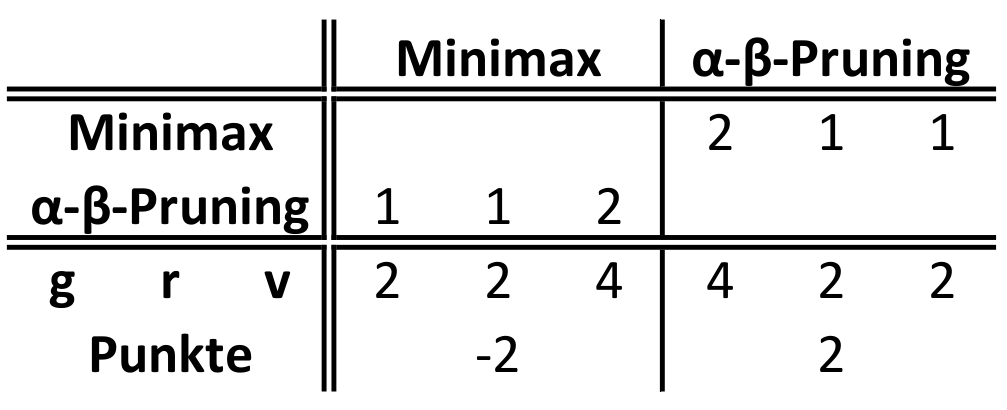
\includegraphics{../images/nmm-mm-vs-ab.png}

Die vorherige Vermutung lässt sich mit diesem Ergebnis bestätigen:
\emph{$\alpha$-$\beta$-Pruning} schneidet besser ab als \emph{Minimax}. Dennoch ist
es überraschend, dass zwei der Spiele im Remis enden und weitere zwei
Spiele sogar von Minimax gewonnen werden.

Zu dem Gesamtsieg von \emph{$\alpha$-$\beta$-Pruning} hat einerseits der Algorithmus
selbst beigetragen, da dadurch weite Teile des Suchbaumes übersprungen
werden konnten. Die Verwendung der \emph{iterativen Tiefensuche} hat mit
einer festen Suchgröße dazu beigetragen, dass bei gleichbleibender
Rechenzeit dynamisch die richtige Rekursionstiefe gewählt werden konnte.
Die Erkennung von symmetrischen Zuständen hilft besonders in den ersten
Zügen eine große Rekursionstiefe zu erreichen, da hier viele Symmetrien
auftauchen. Auch in der letzten fliegenden Phase können ein paar
Rechnungen damit eingespaart werden.

    \hypertarget{heuristik-vs.heuristik-ux3b1-ux3b2-pruning}{%
\subsubsection{Heuristik vs.~Heuristik
($\alpha$-$\beta$-Pruning)}\label{heuristik-vs.heuristik-ux3b1-ux3b2-pruning}}

In dem zweiten Experiment soll unter Verwendung des $\alpha$-$\beta$-Pruning
Algorithmus herausgefunden werden, welche Heuristik am besten geeignet
ist. Die Anzahl der möglichen Heuristiken ist unendlich groß, da jeder
der vier Parameter eine reelle Zahl ist. Aus diesem Grund soll nur ein
kleines Experiment durchgeführt werden. Es treten sechs Konfigurationen
in 3 Spielen pro Runde an. Dadurch ergibt sich eine Rundenanzahl von 30.

Bei diesem Experiment soll die Wichtigkeit der Parameter festgestellt
werden, indem alle möglichen Heuristiken mit den Permutationen der
Zahlen \(1, 2, 3\) gegeneinander antreten. Die Parameter \texttt{stones}
und \texttt{stash} erhalten jedoch immer den gleichen Wert, da sich
während der Entwicklung gezeigt hat, dass die Algorithmen besonders in
der ersten Phase falsche Entscheidungen treffen, sollten sich diese
Parameter unterscheiden. Als positiver Nebeneffekt verringert sich die
Größe des Experimentes.

    \begin{tcolorbox}[breakable, size=fbox, boxrule=1pt, pad at break*=1mm,colback=cellbackground, colframe=cellborder]
\prompt{In}{incolor}{ }{\boxspacing}
\begin{Verbatim}[commandchars=\\\{\}]
\PY{n}{Tournament}\PY{p}{(}
    \PY{p}{[}
        \PY{k}{lambda}\PY{p}{:} \PY{n}{AlphaBetaPruning}\PY{p}{(}\PY{n}{weights}\PY{o}{=}\PY{n}{HeuristicWeights}\PY{p}{(}\PY{n}{stones}\PY{o}{=}\PY{l+m+mi}{1}\PY{p}{,} \PY{n}{stash}\PY{o}{=}\PY{l+m+mi}{1}\PY{p}{,} \PY{n}{mills}\PY{o}{=}\PY{l+m+mi}{2}\PY{p}{,} \PY{n}{possible\PYZus{}mills}\PY{o}{=}\PY{l+m+mi}{3}\PY{p}{)}\PY{p}{)}\PY{p}{,}
        \PY{k}{lambda}\PY{p}{:} \PY{n}{AlphaBetaPruning}\PY{p}{(}\PY{n}{weights}\PY{o}{=}\PY{n}{HeuristicWeights}\PY{p}{(}\PY{n}{stones}\PY{o}{=}\PY{l+m+mi}{2}\PY{p}{,} \PY{n}{stash}\PY{o}{=}\PY{l+m+mi}{2}\PY{p}{,} \PY{n}{mills}\PY{o}{=}\PY{l+m+mi}{1}\PY{p}{,} \PY{n}{possible\PYZus{}mills}\PY{o}{=}\PY{l+m+mi}{3}\PY{p}{)}\PY{p}{)}\PY{p}{,}
        \PY{k}{lambda}\PY{p}{:} \PY{n}{AlphaBetaPruning}\PY{p}{(}\PY{n}{weights}\PY{o}{=}\PY{n}{HeuristicWeights}\PY{p}{(}\PY{n}{stones}\PY{o}{=}\PY{l+m+mi}{3}\PY{p}{,} \PY{n}{stash}\PY{o}{=}\PY{l+m+mi}{3}\PY{p}{,} \PY{n}{mills}\PY{o}{=}\PY{l+m+mi}{2}\PY{p}{,} \PY{n}{possible\PYZus{}mills}\PY{o}{=}\PY{l+m+mi}{1}\PY{p}{)}\PY{p}{)}\PY{p}{,}
        \PY{k}{lambda}\PY{p}{:} \PY{n}{AlphaBetaPruning}\PY{p}{(}\PY{n}{weights}\PY{o}{=}\PY{n}{HeuristicWeights}\PY{p}{(}\PY{n}{stones}\PY{o}{=}\PY{l+m+mi}{1}\PY{p}{,} \PY{n}{stash}\PY{o}{=}\PY{l+m+mi}{1}\PY{p}{,} \PY{n}{mills}\PY{o}{=}\PY{l+m+mi}{3}\PY{p}{,} \PY{n}{possible\PYZus{}mills}\PY{o}{=}\PY{l+m+mi}{2}\PY{p}{)}\PY{p}{)}\PY{p}{,}
        \PY{k}{lambda}\PY{p}{:} \PY{n}{AlphaBetaPruning}\PY{p}{(}\PY{n}{weights}\PY{o}{=}\PY{n}{HeuristicWeights}\PY{p}{(}\PY{n}{stones}\PY{o}{=}\PY{l+m+mi}{2}\PY{p}{,} \PY{n}{stash}\PY{o}{=}\PY{l+m+mi}{2}\PY{p}{,} \PY{n}{mills}\PY{o}{=}\PY{l+m+mi}{3}\PY{p}{,} \PY{n}{possible\PYZus{}mills}\PY{o}{=}\PY{l+m+mi}{1}\PY{p}{)}\PY{p}{)}\PY{p}{,}
        \PY{k}{lambda}\PY{p}{:} \PY{n}{AlphaBetaPruning}\PY{p}{(}\PY{n}{weights}\PY{o}{=}\PY{n}{HeuristicWeights}\PY{p}{(}\PY{n}{stones}\PY{o}{=}\PY{l+m+mi}{3}\PY{p}{,} \PY{n}{stash}\PY{o}{=}\PY{l+m+mi}{3}\PY{p}{,} \PY{n}{mills}\PY{o}{=}\PY{l+m+mi}{1}\PY{p}{,} \PY{n}{possible\PYZus{}mills}\PY{o}{=}\PY{l+m+mi}{2}\PY{p}{)}\PY{p}{)}\PY{p}{,}
    \PY{p}{]}\PY{p}{,}
    \PY{n}{instances\PYZus{}per\PYZus{}round} \PY{o}{=} \PY{l+m+mi}{3}\PY{p}{,}
    \PY{n}{name}                \PY{o}{=} \PY{l+s+s2}{\PYZdq{}}\PY{l+s+s2}{hr\PYZhy{}vs\PYZhy{}hr}\PY{l+s+s2}{\PYZdq{}}\PY{p}{,}
\PY{p}{)}\PY{o}{.}\PY{n}{play}\PY{p}{(}\PY{p}{)}
\end{Verbatim}
\end{tcolorbox}

    Die Rechenzeit für dieses Experiment betrug ca. 12 Stunden. Dabei
reichte zwischenzeitlich der Arbeitsspeicher von 32GB nicht aus und das
Experiment brach kurzzeitig ab.

Die aggregierten Ergebnisse sind in der folgenden Tabelle dargestellt.
Die detaillierten Ergebnisse sind in den Dateien
\texttt{round-hr-vs-hr-\{1-30\}.txt} zu finden. Die Spalten stellen die
\emph{weißen} Spieler dar und die Zeilen die \emph{schwarzen} Spieler.
Jede Heuristik hat einmal als \emph{weiß} und einmal als \emph{schwarz}
gegen jede andere Heuristik gespielt. Gegen sich selbst wurde nicht
gespielt (siehe Diagonale ohne Daten).

Der Bezeichner für jede Heurisik ist als Tupel aufgeschrieben, die
folgender Definition entspricht:
\[\langle stones, stash, mills, possible\_mills \rangle\] Eine Zelle in
der Tabelle stellt eine Runde dar und zählt die Anzahl der Spiele in
drei Kategorien: \[Weiß\ gewinnt\ |\ Remis\ |\ Schwarz\ gewinnt\]

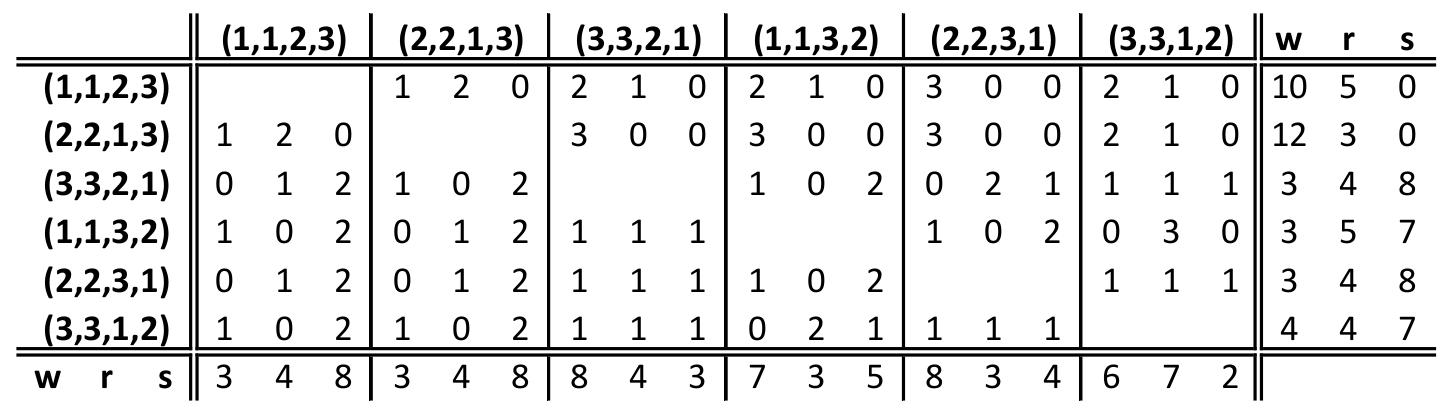
\includegraphics{../images/nmm-hr-vs-hr-rounds.png}

Aggregiert ergibt sich aus den Rundenergebnissen folgende Tabelle. Alle
Spiele der Heuristiken wurden aufgeschlüsselt in
\[Gewonnen\ |\ Remis\ |\ Verloren \] Für die Punkteberechnung wurde
jedes Gewinnen mit \(+1\) und jedes Verlieren mit \(-1\) bewertet. Ein
Remis hat eine Wertung von \(0\).

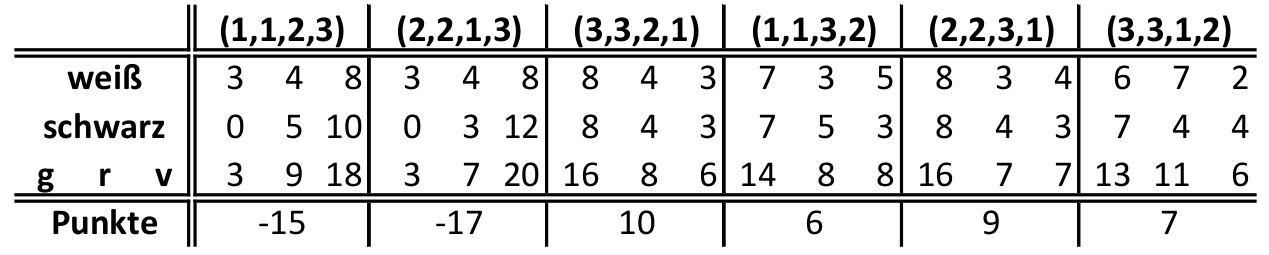
\includegraphics{../images/nmm-hr-vs-hr-total.png}

Als klare Verlierer sind die Heuristiken zu bewerten, welche den
Parameter \(possible\_mills\) größer als die anderen Parameter gewählt
haben. Beide haben mehr als die Hälfte der 30 gespielten Spiele verloren
und haben somit auch eine sehr negative Punktwertung.

Mit einem Punkt Vorsprung gewinnt die Heuristik
\(\langle 3,3,2,1 \rangle\) in der Gesamtwertung. Diese gewichtet
\(stones\) und \(stash\) höher als \(mills\), welche wiederum höher als
\(possible\_mills\) gewichtet werden. Der zweite Platz
\(\langle 2,2,3,1 \rangle\) verliert nur mit einem Punkt. Auch im
direkten Vergleich gewann der erste Platz nur einmal öfter gegen den
zweiten Platz.

Da diese Werte sehr nah aneinander liegen, können diese kleinen
Abweichungen auch durch Zufall entstanden sein. Bei gleich bewerteten
Zügen wählt der Algorithmus einen Spielzug zufällig aus.

    \hypertarget{verbesserungsmuxf6glichkeiten}{%
\subsection{Verbesserungsmöglichkeiten}\label{verbesserungsmuxf6glichkeiten}}

Die Implementierung benötigt sehr viel Arbeitsspeicher, was jedoch beim
normalen Spielen kein Problem darstellen sollte. Erst wenn zu
Testzwecken mehrere Spiele gleichzeitig gespielt werden, macht sich der
große Arbeitsspeicherverbrauch bemerkbar. Durch die Verwendung einer
Bitmaske könnte der Arbeitsspeicher um ein Vielfaches verringert werden.
Die Änderung hätte aber eine komplette Neuimplementierung erfordert,
welche den Rahmen der Studienarbeit gesprengt hätte.

Die Rechenzeit der Algorithmen ist sehr hoch. Dies hängt stark mit dem
Arbeitsspeicherverbrauch zusammen, da hierdurch mehr Daten kopiert
werden müssen und Berechnungen auf Grund der größeren Datenmengen länger
brauchen. Eine Verringerung der Rechenzeit könnte die Algorithmen aus
Sicht des Anwenders besser werden lassen, da in der gleichen Zeit mehr
Zustände in einer größeren Rekursionstiefe, und damit weitere Züge in
der Zukunft, betrachtet werden.

Das Lösen dieser Probleme würde eine komplette Neuimplementierung der
Algorithmen nötig machen. Im gleichen Zuge könnte dann jedoch eine
schnellere, kompilierte Sprache für die Implementierung gewählt werden,
beispielsweise \emph{C}, \emph{C++} oder \emph{Rust}.


    % Add a bibliography block to the postdoc
    
    
    
\end{document} 